\documentclass[10pt,adobefonts,fancyhdr,hyperref,UTF8]{ctexbook}

\usepackage{multirow}
% for \soul 刪除線
\usepackage{ulem}
% 表頭斜線
\usepackage{diagbox}

\makeatletter
\usepackage[centering,paperwidth=180mm,paperheight=230mm,%
body={390pt,530pt},marginparsep=10pt,marginpar=50pt]{geometry}
\usepackage{color}
\usepackage{enumitem}
\usepackage{fancyvrb}
\usepackage[bottom,perpage,symbol*]{footmisc}
\usepackage{graphicx}
\usepackage[hidelinks]{hyperref}
\usepackage{makeidx}
\usepackage[toc]{multitoc}
\usepackage{pifont}
\usepackage{underscore}
\usepackage{amsmath}

\DefineFNsymbols*{chinese}{{\ding{172}}{\ding{173}}{\ding{174}}{\ding{175}}%
{\ding{176}}{\ding{177}}{\ding{178}}{\ding{179}}{\ding{180}}{\ding{181}}}
\setfnsymbol{chinese}

\hypersetup{bookmarksnumbered=true,bookmarksdepth=2}

\CTEXsetup[number={\thechapter}]{chapter}
\CTEXsetup[format+={\raggedleft}]{chapter}
\CTEXsetup[beforeskip={10pt}]{chapter}
\CTEXsetup[afterskip={30pt}]{chapter}
\def\CTEX@chapter@aftername{\par} % \CTEXsetup[aftername={\par}]{chapter}
\CTEXsetup[format+={\raggedright}]{section}
\CTEXsetup[beforeskip={-3.0ex plus -1ex minus -.2ex}]{section}
\CTEXsetup[afterskip={2.3ex plus .2ex minus 0.2ex}]{section}

\renewcommand \thefigure{\thechapter-\arabic{figure}}
\renewcommand \thetable{\thechapter-\arabic{table}}

\newcommand\figcaption[1]{\def\@captype{figure}\caption{#1}}
\newcommand\tabcaption[1]{\def\@captype{table}\caption{#1}}

\long\def\@caption#1[#2]#3{%
  \addcontentsline{\csname ext@#1\endcsname}{#1}%
    {\protect\numberline{\csname fnum@#1\endcsname}{ \ignorespaces #2}}% change "the" to "fnum@"
    \normalsize
    \@makecaption{\csname fnum@#1\endcsname}{\ignorespaces #3}}

\long\def\@makecaption#1#2{%
  \vskip\abovecaptionskip
  \sbox\@tempboxa{#1\quad#2}%
  \ifdim \wd\@tempboxa >\hsize
    #1\quad#2\par
  \else
    \global \@minipagefalse
    \hb@xt@\hsize{\hfil\box\@tempboxa\hfil}%
  \fi
  \vskip\belowcaptionskip}

\setlength\abovecaptionskip{0pt}
  
\setmainfont{Times New Roman}
%\setmainfont{Linux Libertine}
%\setmainfont{TeX Gyre Pagella}
\newfontfamily\urlfont{Sans Narrow}
%\setmonofont[AutoFakeBold=1.6,AutoFakeSlant=0.17,Mapping=tex-text-tt]{Inconsolata}
\setCJKfamilyfont{zhyou}{YouYuan}

\newcommand{\fn}[1]{\texttt{#1}}
\newcommand{\sfn}[1]{\texttt{\small #1}}
\newcommand{\kw}[1]{\textsf{#1}}
\newcommand{\myurl}[1]{{\urlfont #1}}
\newcommand{\mpar}[1]{\marginpar[\hfill\kaishu #1]{\kaishu #1}}
\newcommand{\mn}[1]{\texttt{\bs #1}}
\renewcommand{\today}{\the\year-\the\month-\the\day}
\newcommand\bs{\textbackslash}
\newcommand{\code}[1]{\small{\fontspec{Latin Modern Mono} #1}}

\newcommand\begindot{\begin{itemize}
[itemsep=2pt plus 2pt minus 2pt,%
topsep=3pt plus 2pt minus 2pt,%
parsep=0pt plus 2pt minus 2pt]}
\newcommand\myenddot{\end{itemize}}

\newcommand\beginnum{\begin{enumerate}
[itemsep=2pt plus 2pt minus 2pt,%
topsep=3pt plus 2pt minus 2pt,%
parsep=0pt plus 2pt minus 2pt]}
\newcommand\myendnum{\end{enumerate}}

\DefineVerbatimEnvironment%
  {Code}{Verbatim}
  {fontsize=\small,baselinestretch=0.9,xleftmargin=3mm}

\raggedbottom
%\setlength{\parskip}{1ex plus .5ex minus .5ex}

\input{verbatim.cls}
\DefineVerbatimEnvironment%
  {Codex}{Verbatim}
  {fontsize=\small,baselinestretch=0.9,xleftmargin=3mm,%
  frame=lines,labelposition=all,framesep=5pt}

\DefineVerbatimEnvironment%
  {Code}{Verbatim}
  {fontsize=\small,baselinestretch=0.9,xleftmargin=3mm}

\makeindex

\makeatother

\begin{document}
\sloppy
\newcommand\BookTitle{LeetCode題解}
\pagestyle{fancy}
\fancyhf{}
\fancyhead[RE]{\normalfont\small\rmfamily\nouppercase{\leftmark}}
\fancyhead[LO]{\normalfont\small\rmfamily\nouppercase{\rightmark}}
\fancyhead[LE,RO]{\thepage}
%\fancyfoot[LE,LO]{\small\normalfont\youyuan\BookTitle}
%\fancyfoot[RE,RO]{\textsf{\small \color{blue} https://github.com/soulmachine/leetcode}}

\makeatletter
\@openrightfalse
\makeatother

\frontmatter % 開始前言目錄,頁碼用羅馬數字

\thispagestyle{plain}
\begin{center}
  {\LARGE\textbf{\BookTitle}}

  \vspace{1em}
  {\large 靈魂機器 (soulmachine@gmail.com)}

  \vspace{1ex}
  \myurl{https://github.com/soulmachine/leetcode}
  
  \vspace{1ex}
  最後更新 \today
  
  \vspace{1em}
  \textbf{\large 版權聲明}
\end{center}
\noindent 本作品採用“Creative Commons 署名-非商業性使用-相同方式共享 3.0 Unported許可協議 
(cc by-nc-sa)”進行許可。
\texttt{\small http://creativecommons.org/licenses/by-nc-sa/3.0/}

\vspace{1em}
\subsubsection{內容簡介}
本書的目標讀者是準備去北美找工作的碼農,也適用於在國內找工作的碼農,以及剛接觸ACM算法競賽的新手。

本書包含了 LeetCode Online Judge(\myurl{http://leetcode.com/onlinejudge})所有題目的答案,
所有代碼經過精心編寫,編碼規範良好,適合讀者反覆揣摩,模仿,甚至在紙上默寫。

全書的代碼,使用C++ 11的編寫,並在 LeetCode Online Judge 上測試通過。本書中的代碼規範,跟在公司中的工程規範略有不同,為了使代碼短(方便迅速實現):

\begindot
\item 所有代碼都是單一文件。這是因為一般OJ網站,提交代碼的時候只有一個文本框,如果還是
按照標準做法,比如分為頭文件.h和源代碼.cpp,無法在網站上提交;

\item Shorter is better。能遞歸則一定不用棧;能用STL則一定不自己實現。

\item 不提倡防禦式編程。不需要檢查malloc()/new 返回的指針是否為nullptr;不需要檢查內部函數入口參數的有效性。
\myenddot

本手冊假定讀者已經學過《數據結構》\footnote{《數據結構》,嚴蔚敏等著,清華大學出版社,
\myurl{http://book.douban.com/subject/2024655/}},
《算法》\footnote{《Algorithms》,Robert Sedgewick, Addison-Wesley Professional, \myurl{http://book.douban.com/subject/4854123/}}
這兩門課,熟練掌握C++或Java。

\subsubsection{GitHub地址}
本書是開源的,GitHub地址:\myurl{https://github.com/soulmachine/leetcode}

\subsubsection{北美求職微博羣}
我和我的小夥伴們在這裏:\myurl{http://q.weibo.com/1312378}


\tableofcontents

\mainmatter % 開始正文,頁碼用阿拉伯數字

\graphicspath{{images/}}

\chapter{編程技巧}

在判斷兩個浮點數a和b是否相等時,不要用\fn{a==b},應該判斷二者之差的絕對值\fn{fabs(a-b)}是否小於某個閾值,例如\fn{1e-9}。

判斷一個整數是否是為奇數,用\fn{x \% 2 != 0},不要用\fn{x \% 2 == 1},因為x可能是負數。

用\fn{char}的值作為數組下標(例如,統計字符串中每個字符出現的次數),要考慮到\fn{char}可能是負數。有的人考慮到了,先強制轉型為\fn{unsigned int}再用作下標,這仍然是錯的。正確的做法是,先強制轉型為\fn{unsigned char},再用作下標。這涉及C++整型提升的規則,就不詳述了。

以下是關於STL使用技巧的,很多條款來自《Effective STL》這本書。

\subsubsection{vector和string優先於動態分配的數組}

首先,在性能上,由於\fn{vector}能夠保證連續內存,因此一旦分配了後,它的性能跟原始數組相當;

其次,如果用new,意味着你要確保後面進行了delete,一旦忘記了,就會出現BUG,且這樣需要都寫一行delete,代碼不夠短;

再次,聲明多維數組的話,只能一個一個new,例如:
\begin{Code}
int** ary = new int*[row_num];
for(int i = 0; i < row_num; ++i)
    ary[i] = new int[col_num];
\end{Code}
用vector的話一行代碼搞定,
\begin{Code}
vector<vector<int> > ary(row_num, vector<int>(col_num, 0));
\end{Code}

\subsubsection{使用reserve來避免不必要的重新分配}

\chapter{線性表}
這類題目考察線性表的操作,例如,數組,單鏈表,雙向鏈表等。
\newline


\section{數組} %%%%%%%%%%%%%%%%%%%%%%%%%%%%%%


\subsection{Remove Duplicates from Sorted Array}
\label{sec:remove-duplicates-from-sorted-array}


\subsubsection{描述}
Given a sorted array, remove the duplicates in place such that each element appear only once and return the new length.

Do not allocate extra space for another array, you must do this in place with constant memory.

For example, Given input array \code{A = [1,1,2]},

Your function should return length = 2, and A is now \code{\[1,2\]}.


\subsubsection{分析}
無


\subsubsection{代碼1}
\begin{Code}
// LeetCode, Remove Duplicates from Sorted Array
// 時間複雜度O(n),空間複雜度O(1)
class Solution {
public:
    int removeDuplicates(vector<int>& nums) {
        if (nums.empty()) return 0;

        int index = 0;
        for (int i = 1; i < nums.size(); i++) {
            if (nums[index] != nums[i])
                nums[++index] = nums[i];
        }
        return index + 1;
    }
};
\end{Code}


\subsubsection{代碼2}
\begin{Code}
// LeetCode, Remove Duplicates from Sorted Array
// 使用STL,時間複雜度O(n),空間複雜度O(1)
class Solution {
public:
    int removeDuplicates(vector<int>& nums) {
        return distance(nums.begin(), unique(nums.begin(), nums.end()));
    }
};
\end{Code}


\subsubsection{代碼3}
\begin{Code}
// LeetCode, Remove Duplicates from Sorted Array
// 使用STL,時間複雜度O(n),空間複雜度O(1)
class Solution {
public:
    int removeDuplicates(vector<int>& nums) {
        return distance(nums.begin(), removeDuplicates(nums.begin(), nums.end(), nums.begin()));
    }

    template<typename InIt, typename OutIt>
    OutIt removeDuplicates(InIt first, InIt last, OutIt output) {
        while (first != last) {
            *output++ = *first;
            first = upper_bound(first, last, *first);
        }

        return output;
    }
};
\end{Code}


\subsubsection{相關題目}

\begindot
\item Remove Duplicates from Sorted Array II,見 \S \ref{sec:remove-duplicates-from-sorted-array-ii}
\myenddot


\subsection{Remove Duplicates from Sorted Array II}
\label{sec:remove-duplicates-from-sorted-array-ii}


\subsubsection{描述}
Follow up for "Remove Duplicates":
What if duplicates are allowed at most twice?

For example,
Given sorted array \code{A = [1,1,1,2,2,3]},

Your function should return length = 5, and A is now \code{\[1,1,2,2,3\]}


\subsubsection{分析}
加一個變量記錄一下元素出現的次數即可。這題因為是已經排序的數組,所以一個變量即可解決。如果是沒有排序的數組,則需要引入一個hashmap來記錄出現次數。


\subsubsection{代碼1}
\begin{Code}
// LeetCode, Remove Duplicates from Sorted Array II
// 時間複雜度O(n),空間複雜度O(1)
// @author hex108 (https://github.com/hex108)
class Solution {
public:
    int removeDuplicates(vector<int>& nums) {
        if (nums.size() <= 2) return nums.size();

        int index = 2;
        for (int i = 2; i < nums.size(); i++){
            if (nums[i] != nums[index - 2])
                nums[index++] = nums[i];
        }

        return index;
    }
};
\end{Code}


\subsubsection{代碼2}
下面是一個更簡潔的版本。上面的代碼略長,不過擴展性好一些,例如將\fn{occur < 2}改為\fn{occur < 3},就變成了允許重複最多3次。
\begin{Code}
// LeetCode, Remove Duplicates from Sorted Array II
// @author 虞航仲 (http://weibo.com/u/1666779725)
// 時間複雜度O(n),空間複雜度O(1)
class Solution {
public:
    int removeDuplicates(vector<int>& nums) {
        const int n = nums.size();
        int index = 0;
        for (int i = 0; i < n; ++i) {
            if (i > 0 && i < n - 1 && nums[i] == nums[i - 1] && nums[i] == nums[i + 1])
                continue;

            nums[index++] = nums[i];
        }
        return index;
    }
};
\end{Code}


\subsubsection{代碼3}
Variable of duplication
\begin{Code}
// LeetCode, Remove Duplicates from Sorted Array II
// @author
// 時間複雜度O(n),空間複雜度O(1)
class Solution {
public:
    int removeDuplicates(vector<int>& nums, int du) {
        int index = du;
        for (int i = du; i < (int)nums.size(); i++) {
            if (nums[index - du] != nums[i])
                nums[index++] = nums[i];
        }

        return index;
    }
};
\end{Code}
\subsubsection{相關題目}

\begindot
\item Remove Duplicates from Sorted Array,見 \S \ref{sec:remove-duplicates-from-sorted-array}
\myenddot


\subsection{Search in Rotated Sorted Array}
\label{sec:search-in-rotated-sorted-array}


\subsubsection{描述}
Suppose a sorted array is rotated at some pivot unknown to you beforehand.

(i.e., \code{0 1 2 4 5 6 7} might become \code{4 5 6 7 0 1 2}).

You are given a target value to search. If found in the array return its index, otherwise return -1.

You may assume no duplicate exists in the array.


\subsubsection{分析}
二分查找,難度主要在於左右邊界的確定。


\subsubsection{代碼}
\begin{Code}
// LeetCode, Search in Rotated Sorted Array
// 時間複雜度O(log n),空間複雜度O(1)
class Solution {
public:
    int search(const vector<int>& nums, int target) {
        int first = 0, last = nums.size();
        while (first != last) {
            const int mid = first  + (last - first) / 2;
            if (nums[mid] == target)
                return mid;
            if (nums[first] <= nums[mid]) {
                if (nums[first] <= target && target < nums[mid])
                    last = mid;
                else
                    first = mid + 1;
            } else {
                if (nums[mid] < target && target <= nums[last-1])
                    first = mid + 1;
                else
                    last = mid;
            }
        }
        return -1;
    }
};
\end{Code}


\subsubsection{相關題目}

\begindot
\item Search in Rotated Sorted Array II,見 \S \ref{sec:search-in-rotated-sorted-array-ii}
\myenddot


\subsection{Search in Rotated Sorted Array II}
\label{sec:search-in-rotated-sorted-array-ii}


\subsubsection{描述}
Follow up for "Search in Rotated Sorted Array": What if \emph{duplicates} are allowed?

Would this affect the run-time complexity? How and why?

Write a function to determine if a given target is in the array.


\subsubsection{分析}
允許重複元素,則上一題中如果\fn{A[m]>=A[l]},那麼\fn{[l,m]}為遞增序列的假設就不能成立了,比如\code{\[1,3,1,1,1\]}。

如果\fn{A[m]>=A[l]}不能確定遞增,那就把它拆分成兩個條件:
\begindot
\item 若\fn{A[m]>A[l]},則區間\fn{[l,m]}一定遞增
\item 若\fn{A[m]==A[l]} 確定不了,那就\fn{l++},往下看一步即可。
\myenddot

\subsubsection{代碼}
\begin{Code}
// LeetCode, Search in Rotated Sorted Array II
// 時間複雜度O(n),空間複雜度O(1)
class Solution {
public:
    bool search(const vector<int>& nums, int target) {
        int first = 0, last = nums.size();
        while (first != last) {
            const int mid = first  + (last - first) / 2;
            if (nums[mid] == target)
                return true;
            if (nums[first] < nums[mid]) {
                if (nums[first] <= target && target < nums[mid])
                    last = mid;
                else
                    first = mid + 1;
            } else if (nums[first] > nums[mid]) {
                if (nums[mid] < target && target <= nums[last-1])
                    first = mid + 1;
                else
                    last = mid;
            } else
                //skip duplicate one
                first++;
        }
        return false;
    }
};
\end{Code}


\subsubsection{相關題目}

\begindot
\item Search in Rotated Sorted Array,見 \S \ref{sec:search-in-rotated-sorted-array}
\myenddot


\subsection{Median of Two Sorted Arrays}
\label{sec:median-of-two-sorted-arrays}


\subsubsection{描述}
There are two sorted arrays A and B of size m and n respectively. Find the median of the two sorted arrays. The overall run time complexity should be $O(\log (m+n))$.


\subsubsection{分析}
這是一道非常經典的題。這題更通用的形式是,給定兩個已經排序好的數組,找到兩者所有元素中第$k$大的元素。

$O(m+n)$的解法比較直觀,直接merge兩個數組,然後求第$k$大的元素。

不過我們僅僅需要第$k$大的元素,是不需要“排序”這麼昂貴的操作的。可以用一個計數器,記錄當前已經找到第$m$大的元素了。同時我們使用兩個指針\fn{pA}和\fn{pB},分別指向A和B數組的第一個元素,使用類似於merge sort的原理,如果數組A當前元素小,那麼\fn{pA++},同時\fn{m++};如果數組B當前元素小,那麼\fn{pB++},同時\fn{m++}。最終當$m$等於$k$的時候,就得到了我們的答案,$O(k)$時間,$O(1)$空間。但是,當$k$很接近$m+n$的時候,這個方法還是$O(m+n)$的。

有沒有更好的方案呢?我們可以考慮從$k$入手。如果我們每次都能夠刪除一個一定在第$k$大元素之前的元素,那麼我們需要進行$k$次。但是如果每次我們都刪除一半呢?由於A和B都是有序的,我們應該充分利用這裏面的信息,類似於二分查找,也是充分利用了“有序”。

假設A和B的元素個數都大於$k/2$,我們將A的第$k/2$個元素(即\fn{A[k/2-1]})和B的第$k/2$個元素(即\fn{B[k/2-1]})進行比較,有以下三種情況(為了簡化這裏先假設$k$為偶數,所得到的結論對於$k$是奇數也是成立的):
\begindot
\item \fn{A[k/2-1] == B[k/2-1]}
\item \fn{A[k/2-1] > B[k/2-1]}
\item \fn{A[k/2-1] < B[k/2-1]}
\myenddot

如果\fn{A[k/2-1] < B[k/2-1]},意味着\fn{A[0]}到\fn{A[k/2-1]}的肯定在$A \cup B$的top k元素的範圍內,換句話説,\fn{A[k/2-1]}不可能大於$A \cup B$的第$k$大元素。留給讀者證明。

因此,我們可以放心的刪除A數組的這$k/2$個元素。同理,當\fn{A[k/2-1] > B[k/2-1]}時,可以刪除B數組的$k/2$個元素。

當\fn{A[k/2-1] == B[k/2-1]}時,説明找到了第$k$大的元素,直接返回\fn{A[k/2-1]}或\fn{B[k/2-1]}即可。

因此,我們可以寫一個遞歸函數。那麼函數什麼時候應該終止呢?
\begindot
\item 當A或B是空時,直接返回\fn{B[k-1]}或\fn{A[k-1]};
\item 當\fn{k=1}是,返回\fn{min(A[0], B[0])};
\item 當\fn{A[k/2-1] == B[k/2-1]}時,返回\fn{A[k/2-1]}或\fn{B[k/2-1]}
\myenddot


\subsubsection{代碼}
\begin{Code}
// LeetCode, Median of Two Sorted Arrays
// 時間複雜度O(log(m+n)),空間複雜度O(log(m+n))
class Solution {
public:
    double findMedianSortedArrays(const vector<int>& A, const vector<int>& B) {
        const int m = A.size();
        const int n = B.size();
        int total = m + n;
        if (total & 0x1)
            return find_kth(A.begin(), m, B.begin(), n, total / 2 + 1);
        else
            return (find_kth(A.begin(), m, B.begin(), n, total / 2)
                    + find_kth(A.begin(), m, B.begin(), n, total / 2 + 1)) / 2.0;
    }
private:
    static int find_kth(std::vector<int>::const_iterator A, int m,
            std::vector<int>::const_iterator B, int n, int k) {
        //always assume that m is equal or smaller than n
        if (m > n) return find_kth(B, n, A, m, k);
        if (m == 0) return *(B + k - 1);
        if (k == 1) return min(*A, *B);

        //divide k into two parts
        int ia = min(k / 2, m), ib = k - ia;
        if (*(A + ia - 1) < *(B + ib - 1))
            return find_kth(A + ia, m - ia, B, n, k - ia);
        else if (*(A + ia - 1) > *(B + ib - 1))
            return find_kth(A, m, B + ib, n - ib, k - ib);
        else
            return A[ia - 1];
    }
};
\end{Code}


\subsubsection{相關題目}

\begindot
\item 無
\myenddot


\subsection{Longest Consecutive Sequence} %%%%%%%%%%%%%%%%%%%%%%%%%%%%%%
\label{sec:longest-consecutive-sequence}


\subsubsection{描述}
Given an unsorted array of integers, find the length of the longest consecutive elements sequence.

For example,
Given \code{\[100, 4, 200, 1, 3, 2\]},
The longest consecutive elements sequence is \code{\[1, 2, 3, 4\]}. Return its length: 4.

Your algorithm should run in $O(n)$ complexity.


\subsubsection{分析}
如果允許$O(n \log n)$的複雜度,那麼可以先排序,可是本題要求$O(n)$。

由於序列裏的元素是無序的,又要求$O(n)$,首先要想到用哈希表。

用一個哈希表 \fn{unordered_map<int, bool> used}記錄每個元素是否使用,對每個元素,以該元素為中心,往左右擴張,直到不連續為止,記錄下最長的長度。


\subsubsection{代碼}
\begin{Code}
// Leet Code, Longest Consecutive Sequence
// 時間複雜度O(n),空間複雜度O(n)
class Solution {
public:
    int longestConsecutive(const vector<int> &nums) {
        unordered_map<int, bool> used;

        for (auto i : nums) used[i] = false;

        int longest = 0;

        for (auto i : nums) {
            if (used[i]) continue;

            int length = 1;

            used[i] = true;

            for (int j = i + 1; used.find(j) != used.end(); ++j) {
                used[j] = true;
                ++length;
            }

            for (int j = i - 1; used.find(j) != used.end(); --j) {
                used[j] = true;
                ++length;
            }

            longest = max(longest, length);
        }

        return longest;
    }
};
\end{Code}

\subsubsection{分析2}
第一直覺是個聚類的操作,應該有union,find的操作.連續序列可以用兩端和長度來表示.
本來用兩端就可以表示,但考慮到查詢的需求,將兩端分別暴露出來.用\fn{unordered_map<int, int> map}來
存儲.原始思路來自於\url{http://discuss.leetcode.com/questions/1070/longest-consecutive-sequence}

\subsubsection{代碼}

\begin{Code}
// Leet Code, Longest Consecutive Sequence
// 時間複雜度O(n),空間複雜度O(n)
// Author: @advancedxy
class Solution {
public:
    int longestConsecutive(vector<int> &nums) {
        unordered_map<int, int> map;
        int size = nums.size();
        int l = 1;
        for (int i = 0; i < size; i++) {
            if (map.find(nums[i]) != map.end()) continue;
            map[nums[i]] = 1;
            if (map.find(nums[i] - 1) != map.end()) {
                l = max(l, mergeCluster(map, nums[i] - 1, nums[i]));
            }
            if (map.find(nums[i] + 1) != map.end()) {
                l = max(l, mergeCluster(map, nums[i], nums[i] + 1));
            }
        }
        return size == 0 ? 0 : l;
    }

private:
    int mergeCluster(unordered_map<int, int> &map, int left, int right) {
        int upper = right + map[right] - 1;
        int lower = left - map[left] + 1;
        int length = upper - lower + 1;
        map[upper] = length;
        map[lower] = length;
        return length;
    }
};
\end{Code}

\subsubsection{相關題目}
\begindot
\item 無
\myenddot


\subsection{Two Sum} %%%%%%%%%%%%%%%%%%%%%%%%%%%%%%
\label{sec:Two-sum}


\subsubsection{描述}
Given an array of integers, find two numbers such that they add up to a specific target number.

The function twoSum should return indices of the two numbers such that they add up to the target, where index1 must be less than index2. Please note that your returned answers (both index1 and index2) are not zero-based.

You may assume that each input would have exactly one solution.

Input:  \code{numbers=\{2, 7, 11, 15\}, target=9}

Output: \code{index1=1, index2=2}


\subsubsection{分析}
方法1:暴力,複雜度$O(n^2)$,會超時

方法2:hash。用一個哈希表,存儲每個數對應的下標,複雜度$O(n)$.

方法3:先排序,然後左右夾逼,排序$O(n\log n)$,左右夾逼$O(n)$,最終$O(n\log n)$。但是注意,這題需要返回的是下標,而不是數字本身,因此這個方法行不通。


\subsubsection{代碼}
\begin{Code}
//LeetCode, Two Sum
// 方法2:hash。用一個哈希表,存儲每個數對應的下標
// 時間複雜度O(n),空間複雜度O(n)
class Solution {
public:
    vector<int> twoSum(vector<int> &nums, int target) {
        unordered_map<int, int> mapping;
        vector<int> result;
        for (int i = 0; i < nums.size(); i++) {
            mapping[nums[i]] = i;
        }
        for (int i = 0; i < nums.size(); i++) {
            const int gap = target - nums[i];
            if (mapping.find(gap) != mapping.end() && mapping[gap] > i) {
                result.push_back(i + 1);
                result.push_back(mapping[gap] + 1);
                break;
            }
        }
        return result;
    }
};
\end{Code}

\subsubsection{代碼}
\begin{Code}
// 時間複雜度O(n),空間複雜度O(n)
class Solution {
public:
    vector<int> twoSum(vector<int>& nums, int target) {
        unordered_map<int, int> cache;
        for (size_t i = 0; i < nums.size(); i++)
        {
            auto it = cache.find(target - nums[i]);
            if (it != cache.end())
            {
                return vector<int>{it->second, (int)i};
            }
            cache.emplace(nums[i], i);
        }

        return vector<int>(); // should not go here
    }
};
\end{Code}


\subsubsection{相關題目}
\begindot
\item 3Sum, 見 \S \ref{sec:3sum}
\item 3Sum Closest, 見 \S \ref{sec:3sum-closest}
\item 4Sum, 見 \S \ref{sec:4sum}
\myenddot

\subsection{Two Sum III} %%%%%%%%%%%%%%%%%%%%%%%%%%%%%%
\label{sec:Two-sum-iii}


\subsubsection{描述}
Design and implement a TwoSum class. It should support the following operations: add and find.

add - Add the number to an internal data structure.
find - Find if there exists any pair of numbers which sum is equal to the value.

Example 1:
\begin{Code}
add(1); add(3); add(5);
find(4) -> true
find(7) -> false
\end{Code}

Example 2:
\begin{Code}
add(3); add(1); add(2);
find(3) -> true
find(6) -> false
\end{Code}

\subsubsection{代碼}
\begin{Code}
// 用一個 hash map,存儲每個數對應的 count
// 時間複雜度O(n),空間複雜度O(n)
class TwoSum {
public:
    /** Initialize your data structure here. */
    TwoSum() {

    }

    /** Add the number to an internal data structure.. */
    void add(int number) {
        m_cache[number]++;
    }

    /** Find if there exists any pair of numbers which sum is equal to the value. */
    bool find(int value) {
        for (const auto& [k, v] : m_cache)
        {
            auto it = m_cache.find(value - k);
            if (it != m_cache.end())
            {
                // 例子: value: 4, k: 2. 當 k == 2 在數組中只出現一次,不能當是答案
                if (value - k == k)
                {
                    if (v > 1)
                        return true;
                    else
                        continue;
                }
                else
                    return true;
            }
        }
        return false;
    }
private:
    unordered_map<int, int> m_cache;
};

/**
 * Your TwoSum object will be instantiated and called as such:
 * TwoSum* obj = new TwoSum();
 * obj->add(number);
 * bool param_2 = obj->find(value);
 */
\end{Code}



\subsection{3Sum} %%%%%%%%%%%%%%%%%%%%%%%%%%%%%%
\label{sec:3sum}


\subsubsection{描述}
Given an array $S$ of $n$ integers, are there elements $a, b, c$ in $S$ such that $a + b + c = 0$? Find all unique triplets in the array which gives the sum of zero.

Note:
\begindot
\item Elements in a triplet $(a,b,c)$ must be in non-descending order. (ie, $a \leq b \leq c$)
\item The solution set must not contain duplicate triplets.
\myenddot

For example, given array \code{S = \{-1 0 1 2 -1 -4\}}.

A solution set is:
\begin{Code}
(-1, 0, 1)
(-1, -1, 2)
\end{Code}


\subsubsection{分析}
先排序,然後左右夾逼,複雜度 $O(n^2)$。

這個方法可以推廣到$k$-sum,先排序,然後做$k-2$次循環,在最內層循環左右夾逼,時間複雜度是 $O(\max\{n \log n, n^{k-1}\})$。


\subsubsection{代碼}
\begin{Code}
// LeetCode, 3Sum
// 先排序,然後左右夾逼,注意跳過重複的數,時間複雜度O(n^2),空間複雜度O(1)
class Solution {
    public:
    vector<vector<int>> threeSum(vector<int>& nums) {
        vector<vector<int>> result;
        if (nums.size() < 3) return result;
        sort(nums.begin(), nums.end());
        const int target = 0;

        auto last = nums.end();
        for (auto i = nums.begin(); i < last-2; ++i) {
            auto j = i+1;
            if (i > nums.begin() && *i == *(i-1)) continue;
            auto k = last-1;
            while (j < k) {
                if (*i + *j + *k < target) {
                    ++j;
                    while(*j == *(j - 1) && j < k) ++j;
                } else if (*i + *j + *k > target) {
                    --k;
                    while(*k == *(k + 1) && j < k) --k;
                } else {
                    result.push_back({ *i, *j, *k });
                    ++j;
                    --k;
                    while(*j == *(j - 1) && *k == *(k + 1) && j < k) ++j;
                }
            }
        }
        return result;
    }
};
\end{Code}


\subsubsection{相關題目}
\begindot
\item Two sum, 見 \S \ref{sec:Two-sum}
\item 3Sum Closest, 見 \S \ref{sec:3sum-closest}
\item 4Sum, 見 \S \ref{sec:4sum}
\myenddot

\subsection{3Sum Closest} %%%%%%%%%%%%%%%%%%%%%%%%%%%%%%
\label{sec:3sum-closest}


\subsubsection{描述}
Given an array $S$ of $n$ integers, find three integers in $S$ such that the sum is closest to a given number, target. Return the sum of the three integers. You may assume that each input would have exactly one solution.

For example, given array \code{S = \{-1 2 1 -4\}}, and \code{target = 1}.

The sum that is closest to the target is 2. (\code{-1 + 2 + 1 = 2}).


\subsubsection{分析}
先排序,然後左右夾逼,複雜度 $O(n^2)$。


\subsubsection{代碼}
\begin{Code}
// LeetCode, 3Sum Closest
// 先排序,然後左右夾逼,時間複雜度O(n^2),空間複雜度O(1)
class Solution {
public:
    int threeSumClosest(vector<int>& nums, int target) {
        int result = 0;
        int min_gap = INT_MAX;

        sort(nums.begin(), nums.end());

        for (auto a = nums.begin(); a != prev(nums.end(), 2); ++a) {
            auto b = next(a);
            auto c = prev(nums.end());

            while (b < c) {
                const int sum = *a + *b + *c;
                const int gap = abs(sum - target);

                if (gap < min_gap) {
                    result = sum;
                    min_gap = gap;
                }

                if (sum < target) ++b;
                else              --c;
            }
        }

        return result;
    }
};
\end{Code}


\subsubsection{相關題目}
\begindot
\item Two sum, 見 \S \ref{sec:Two-sum}
\item 3Sum, 見 \S \ref{sec:3sum}
\item 4Sum, 見 \S \ref{sec:4sum}
\myenddot


\subsection{4Sum} %%%%%%%%%%%%%%%%%%%%%%%%%%%%%%
\label{sec:4sum}


\subsubsection{描述}
Given an array $S$ of $n$ integers, are there elements $a, b, c$, and $d$ in $S$ such that $a + b + c + d = target$? Find all unique quadruplets in the array which gives the sum of target.

Note:
\begindot
\item Elements in a quadruplet $(a,b,c,d)$ must be in non-descending order. (ie, $a \leq b \leq c \leq d$)
\item The solution set must not contain duplicate quadruplets.
\myenddot

For example, given array \code{S = \{1 0 -1 0 -2 2\}}, and \code{target = 0}.

A solution set is:
\begin{Code}
(-1,  0, 0, 1)
(-2, -1, 1, 2)
(-2,  0, 0, 2)
\end{Code}


\subsubsection{分析}
先排序,然後左右夾逼,複雜度 $O(n^3)$,會超時。

可以用一個hashmap先緩存兩個數的和,最終複雜度$O(n^3)$。這個策略也適用於 3Sum 。


\subsubsection{左右夾逼}
\begin{Code}
// LeetCode, 4Sum
// 先排序,然後左右夾逼,時間複雜度O(n^3),空間複雜度O(1)
class Solution {
public:
    vector<vector<int>> fourSum(vector<int>& nums, int target) {
        vector<vector<int>> result;
        if (nums.size() < 4) return result;
        sort(nums.begin(), nums.end());

        auto last = nums.end();
        for (auto a = nums.begin(); a < prev(last, 3); ++a) {
            for (auto b = next(a); b < prev(last, 2); ++b) {
                auto c = next(b);
                auto d = prev(last);
                while (c < d) {
                    if (*a + *b + *c + *d < target) {
                        ++c;
                    } else if (*a + *b + *c + *d > target) {
                        --d;
                    } else {
                        result.push_back({ *a, *b, *c, *d });
                        ++c;
                        --d;
                    }
                }
            }
        }
        sort(result.begin(), result.end());
        result.erase(unique(result.begin(), result.end()), result.end());
        return result;
    }
};
\end{Code}


\subsubsection{map做緩存}
\begin{Code}
// LeetCode, 4Sum
// 用一個hashmap先緩存兩個數的和
// 時間複雜度,平均O(n^2),最壞O(n^4),空間複雜度O(n^2)
class Solution {
public:
    vector<vector<int> > fourSum(vector<int> &nums, int target) {
        vector<vector<int>> result;
        if (nums.size() < 4) return result;
        sort(nums.begin(), nums.end());

        unordered_map<int, vector<pair<int, int> > > cache;
        for (size_t a = 0; a < nums.size(); ++a) {
            for (size_t b = a + 1; b < nums.size(); ++b) {
                cache[nums[a] + nums[b]].push_back(pair<int, int>(a, b));
            }
        }

        for (int c = 0; c < nums.size(); ++c) {
            for (size_t d = c + 1; d < nums.size(); ++d) {
                const int key = target - nums[c] - nums[d];
                if (cache.find(key) == cache.end()) continue;

                const auto& vec = cache[key];
                for (size_t k = 0; k < vec.size(); ++k) {
                    if (c <= vec[k].second)
                        continue; // 有重疊

                    result.push_back( { nums[vec[k].first],
                            nums[vec[k].second], nums[c], nums[d] });
                }
            }
        }
        sort(result.begin(), result.end());
        result.erase(unique(result.begin(), result.end()), result.end());
        return result;
    }
};
\end{Code}


\subsubsection{multimap}
\begin{Code}
// LeetCode, 4Sum
// 用一個 hashmap 先緩存兩個數的和
// 時間複雜度O(n^2),空間複雜度O(n^2)
// @author 龔陸安(http://weibo.com/luangong)
class Solution {
public:
    vector<vector<int>> fourSum(vector<int>& nums, int target) {
        vector<vector<int>> result;
        if (nums.size() < 4) return result;
        sort(nums.begin(), nums.end());

        unordered_multimap<int, pair<int, int>> cache;
        for (int i = 0; i + 1 < nums.size(); ++i)
            for (int j = i + 1; j < nums.size(); ++j)
                cache.insert(make_pair(nums[i] + nums[j], make_pair(i, j)));

        for (auto i = cache.begin(); i != cache.end(); ++i) {
            int x = target - i->first;
            auto range = cache.equal_range(x);
            for (auto j = range.first; j != range.second; ++j) {
                auto a = i->second.first;
                auto b = i->second.second;
                auto c = j->second.first;
                auto d = j->second.second;
                if (a != c && a != d && b != c && b != d) {
                    vector<int> vec = { nums[a], nums[b], nums[c], nums[d] };
                    sort(vec.begin(), vec.end());
                    result.push_back(vec);
                }
            }
        }
        sort(result.begin(), result.end());
        result.erase(unique(result.begin(), result.end()), result.end());
        return result;
    }
};
\end{Code}


\subsubsection{方法4}
\begin{Code}
// LeetCode, 4Sum
// 先排序,然後左右夾逼,時間複雜度O(n^3logn),空間複雜度O(1),會超時
// 跟方法1相比,表面上優化了,實際上更慢了,切記!
class Solution {
public:
    vector<vector<int>> fourSum(vector<int>& nums, int target) {
        vector<vector<int>> result;
        if (nums.size() < 4) return result;
        sort(nums.begin(), nums.end());

        auto last = nums.end();
        for (auto a = nums.begin(); a < prev(last, 3);
                a = upper_bound(a, prev(last, 3), *a)) {
            for (auto b = next(a); b < prev(last, 2);
                    b = upper_bound(b, prev(last, 2), *b)) {
                auto c = next(b);
                auto d = prev(last);
                while (c < d) {
                    if (*a + *b + *c + *d < target) {
                        c = upper_bound(c, d, *c);
                    } else if (*a + *b + *c + *d > target) {
                        d = prev(lower_bound(c, d, *d));
                    } else {
                        result.push_back({ *a, *b, *c, *d });
                        c = upper_bound(c, d, *c);
                        d = prev(lower_bound(c, d, *d));
                    }
                }
            }
        }
        return result;
    }
};
\end{Code}


\subsubsection{相關題目}
\begindot
\item Two sum, 見 \S \ref{sec:Two-sum}
\item 3Sum, 見 \S \ref{sec:3sum}
\item 3Sum Closest, 見 \S \ref{sec:3sum-closest}
\myenddot

\subsection{4Sum II} %%%%%%%%%%%%%%%%%%%%%%%%%%%%%%
\label{sec:4sum-ii}


\subsubsection{描述}
Given four lists A, B, C, D of integer values, compute how many tuples (i, j, k, l) there are such that A[i] + B[j] + C[k] + D[l] is zero.

To make problem a bit easier, all A, B, C, D have same length of N where 0 ≤ N ≤ 500. All integers are in the range of -228 to 228 - 1 and the result is guaranteed to be at most 231 - 1.

Example:
\begin{Code}
Input:
A = [ 1, 2]
B = [-2,-1]
C = [-1, 2]
D = [ 0, 2]

Output:
2

Explanation:
The two tuples are:
1. (0, 0, 0, 1) -> A[0] + B[0] + C[0] + D[1] = 1 + (-2) + (-1) + 2 = 0
2. (1, 1, 0, 0) -> A[1] + B[1] + C[0] + D[0] = 2 + (-1) + (-1) + 0 = 0
\end{Code}


\subsubsection{Hash map}
\begin{Code}
class Solution {
public:
    int fourSumCount(vector<int>& A, vector<int>& B, vector<int>& C, vector<int>& D) {
        int cnt = 0;
        // 製造 hash map 來記低數組 A, B
        unordered_map<int, int> m;
        for (int a : A)
            for (int b : B)
                ++m[a + b];

        // 對比數組 C, D
        for (int c : C)
            for (int d : D) {
                auto it = m.find(-(c + d));
                if (it != end(m))
                    cnt += it->second;
            }

        return cnt;
    }
};
\end{Code}

\subsection{Remove Element} %%%%%%%%%%%%%%%%%%%%%%%%%%%%%%
\label{sec:remove-element }


\subsubsection{描述}
Given an array and a value, remove all instances of that value in place and return the new length.

The order of elements can be changed. It doesn't matter what you leave beyond the new length.


\subsubsection{分析}
無


\subsubsection{代碼1}
\begin{Code}
// LeetCode, Remove Element
// 時間複雜度O(n),空間複雜度O(1)
class Solution {
public:
    int removeElement(vector<int>& nums, int target) {
        int index = 0;
        for (int i = 0; i < nums.size(); ++i) {
            if (nums[i] != target) {
                nums[index++] = nums[i];
            }
        }
        return index;
    }
};
\end{Code}


\subsubsection{代碼2}
\begin{Code}
// LeetCode, Remove Element
// 使用remove(),時間複雜度O(n),空間複雜度O(1)
class Solution {
public:
    int removeElement(vector<int>& nums, int target) {
        return distance(nums.begin(), remove(nums.begin(), nums.end(), target));
    }
};
\end{Code}


\subsubsection{相關題目}
\begindot
\item 無
\myenddot


\subsection{Next Permutation} %%%%%%%%%%%%%%%%%%%%%%%%%%%%%%
\label{sec:next-permutation}


\subsubsection{描述}
Implement next permutation, which rearranges numbers into the lexicographically next greater permutation of numbers.

If such arrangement is not possible, it must rearrange it as the lowest possible order (ie, sorted in ascending order).

The replacement must be in-place, do not allocate extra memory.

Here are some examples. Inputs are in the left-hand column and its corresponding outputs are in the right-hand column.
\begin{Code}
1,2,3 → 1,3,2
3,2,1 → 1,2,3
1,1,5 → 1,5,1
\end{Code}


\subsubsection{分析}
算法過程如圖~\ref{fig:permutation}所示(來自\myurl{http://fisherlei.blogspot.com/2012/12/leetcode-next-permutation.html})。

\begin{center}
\includegraphics[width=360pt]{next-permutation.png}\\
\figcaption{下一個排列算法流程}\label{fig:permutation}
\end{center}


\subsubsection{代碼}
\begin{Code}
// LeetCode, Next Permutation
// 時間複雜度O(n),空間複雜度O(1)
class Solution {
public:
    void nextPermutation(vector<int> &nums) {
        next_permutation(nums.begin(), nums.end());
    }

    template<typename BidiIt>
    bool next_permutation(BidiIt first, BidiIt last) {
        // Get a reversed range to simplify reversed traversal.
        const auto rfirst = reverse_iterator<BidiIt>(last);
        const auto rlast = reverse_iterator<BidiIt>(first);

        // Begin from the second last element to the first element.
        auto pivot = next(rfirst);

        // Find `pivot`, which is the first element that is no less than its
        // successor.  `Prev` is used since `pivort` is a `reversed_iterator`.
        while (pivot != rlast && *pivot >= *prev(pivot))
            ++pivot;

        // No such elemenet found, current sequence is already the largest
        // permutation, then rearrange to the first permutation and return false.
        if (pivot == rlast) {
            reverse(rfirst, rlast);
            return false;
        }

        // Scan from right to left, find the first element that is greater than
        // `pivot`.
        auto change = find_if(rfirst, pivot, bind1st(less<int>(), *pivot));

        swap(*change, *pivot);
        reverse(rfirst, pivot);

        return true;
    }
};
\end{Code}


\subsubsection{相關題目}
\begindot
\item Permutation Sequence, 見 \S \ref{sec:permutation-sequence}
\item Permutations, 見 \S \ref{sec:permutations}
\item Permutations II, 見 \S \ref{sec:permutations-ii}
\item Combinations, 見 \S \ref{sec:combinations}
\myenddot

\subsection{Prev Permutation} %%%%%%%%%%%%%%%%%%%%%%%%%%%%%%
\label{sec:prev-permutation}


\subsubsection{描述}
Implement previous permutation

\begin{Code}
1,2,3 → 3,2,1
3,2,1 → 3,1,2
1,1,5 → 5,1,1
\end{Code}


\subsubsection{分析}
無

\subsubsection{代碼}
\begin{Code}
// LeetCode, Previous Permutation
// 時間複雜度O(n),空間複雜度O(1)
class Solution {
public:
    void prevPermutation(vector<int> &nums) {
        prev_permutation(nums.begin(), nums.end());
    }

    template<typename BidiIt>
    bool prev_permutation(BidiIt first, BidiIt last) {
        const auto rfirst = reverse_iterator<BidiIt>(last);
        const auto rlast = reverse_iterator<BidiIt>(first);

        auto pivot = next(rfirst);

        while (pivot != rlast && *(pivot) <= *prev(pivot))
            pivot++;

        if (pivot == rlast) {
            reverse(rfirst, rlast);
            return false;
        }

        auto change = find_if(rfirst, pivot, bind1st(greater<int>(), *pivot));

        swap(*change, *pivot);
        reverse(rfirst, pivot);

        return true;
    }
};
\end{Code}


\subsubsection{相關題目}
\begindot
\item Permutation Sequence, 見 \S \ref{sec:permutation-sequence}
\item Permutations, 見 \S \ref{sec:permutations}
\item Permutations II, 見 \S \ref{sec:permutations-ii}
\item Combinations, 見 \S \ref{sec:combinations}
\myenddot

\subsection{Permutation Sequence} %%%%%%%%%%%%%%%%%%%%%%%%%%%%%%
\label{sec:permutation-sequence}


\subsubsection{描述}
The set \fn{[1,2,3,…,n]} contains a total of $n!$ unique permutations.

By listing and labeling all of the permutations in order,
We get the following sequence (ie, for $n = 3$):
\begin{Code}
"123"
"132"
"213"
"231"
"312"
"321"
\end{Code}

Given $n$ and $k$, return the kth permutation sequence.

Note: Given $n$ will be between 1 and 9 inclusive.


\subsubsection{分析}
簡單的,可以用暴力枚舉法,調用 $k-1$ 次 \fn{next_permutation()}。

暴力枚舉法把前 $k$個排列都求出來了,比較浪費,而我們只需要第$k$個排列。

利用康託編碼的思路,假設有$n$個不重複的元素,第$k$個排列是$a_1, a_2, a_3, ..., a_n$,那麼$a_1$是哪一個位置呢?

我們把$a_1$去掉,那麼剩下的排列為
$a_2, a_3, ..., a_n$, 共計$n-1$個元素,$n-1$個元素共有$(n-1)!$個排列,於是就可以知道 $a_1 = k / (n-1)!$。

同理,$a_2, a_3, ..., a_n$的值推導如下:

\begin{eqnarray}
k_2 &=& k\%(n-1)! \nonumber \\
a_2 &=& k_2/(n-2)! \nonumber \\
\quad & \cdots \nonumber \\
k_{n-1} &=& k_{n-2}\%2! \nonumber \\
a_{n-1} &=& k_{n-1}/1! \nonumber \\
a_n &=& 0 \nonumber
\end{eqnarray}


\subsubsection{使用next_permutation()}
\begin{Code}
// LeetCode, Permutation Sequence
// 使用next_permutation(),TLE
class Solution {
public:
    string getPermutation(int n, int k) {
        string s(n, '0');
        for (int i = 0; i < n; ++i)
            s[i] += i+1;
        for (int i = 0; i < k-1; ++i)
            next_permutation(s.begin(), s.end());
        return s;
    }

    template<typename BidiIt>
    bool next_permutation(BidiIt first, BidiIt last) {
        // 代碼見上一題 Next Permutation
    }
};
\end{Code}


\subsubsection{康託編碼}
\begin{Code}
// LeetCode, Permutation Sequence
// 康託編碼,時間複雜度O(n),空間複雜度O(1)
class Solution {
public:
    string getPermutation(int n, int k) {
        string s(n, '0');
        string result;
        for (int i = 0; i < n; ++i)
            s[i] += i + 1;

        return kth_permutation(s, k);
    }
private:
    int factorial(int n) {
        int result = 1;
        for (int i = 1; i <= n; ++i)
            result *= i;
        return result;
    }

    // seq 已排好序,是第一個排列
    template<typename Sequence>
    Sequence kth_permutation(const Sequence &seq, int k) {
        const int n = seq.size();
        Sequence S(seq);
        Sequence result;

        int base = factorial(n - 1);
        --k;  // 康託編碼從0開始

        for (int i = n - 1; i > 0; k %= base, base /= i, --i) {
            auto a = next(S.begin(), k / base);
            result.push_back(*a);
            S.erase(a);
        }

        result.push_back(S[0]); // 最後一個
        return result;
    }
};
\end{Code}


\subsubsection{相關題目}
\begindot
\item Next Permutation, 見 \S \ref{sec:next-permutation}
\item Permutations, 見 \S \ref{sec:permutations}
\item Permutations II, 見 \S \ref{sec:permutations-ii}
\item Combinations, 見 \S \ref{sec:combinations}
\myenddot


\subsection{Valid Sudoku} %%%%%%%%%%%%%%%%%%%%%%%%%%%%%%
\label{sec:valid-sudoku}


\subsubsection{描述}
Determine if a Sudoku is valid, according to: Sudoku Puzzles - The Rules \myurl{http://sudoku.com.au/TheRules.aspx} .

The Sudoku board could be partially filled, where empty cells are filled with the character \fn{'.'}.

\begin{center}
\includegraphics[width=150pt]{sudoku.png}\\
\figcaption{A partially filled sudoku which is valid}\label{fig:sudoku}
\end{center}

\subsubsection{分析}
細節實現題。


\subsubsection{代碼}
\begin{Code}
// LeetCode, Valid Sudoku
// 時間複雜度O(n^2),空間複雜度O(1)
class Solution {
public:
    bool isValidSudoku(const vector<vector<char>>& board) {
        bool used[9];

        for (int i = 0; i < 9; ++i) {
            fill(used, used + 9, false);

            for (int j = 0; j < 9; ++j) // 檢查行
                if (!check(board[i][j], used))
                    return false;

            fill(used, used + 9, false);

            for (int j = 0; j < 9; ++j) // 檢查列
                if (!check(board[j][i], used))
                    return false;
        }

        for (int r = 0; r < 3; ++r) // 檢查 9 個子格子
            for (int c = 0; c < 3; ++c) {
                fill(used, used + 9, false);

                for (int i = r * 3; i < r * 3 + 3; ++i)
                    for (int j = c * 3; j < c * 3 + 3; ++j)
                        if (!check(board[i][j], used))
                            return false;
            }

        return true;
    }

    bool check(char ch, bool used[9]) {
        if (ch == '.') return true;

        if (used[ch - '1']) return false;

        return used[ch - '1'] = true;
    }
};
\end{Code}


\subsubsection{相關題目}
\begindot
\item Sudoku Solver, 見 \S \ref{sec:sudoku-solver}
\myenddot


\subsection{Trapping Rain Water} %%%%%%%%%%%%%%%%%%%%%%%%%%%%%%
\label{sec:trapping-rain-water}


\subsubsection{描述}
Given $n$ non-negative integers representing an elevation map where the width of each bar is 1, compute how much water it is able to trap after raining.

For example,
Given \code{\[0,1,0,2,1,0,1,3,2,1,2,1\]}, return 6.

\begin{center}
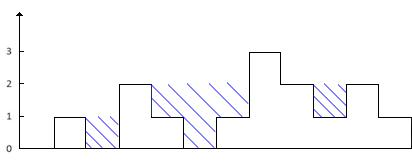
\includegraphics{trapping-rain-water.png}\\
\figcaption{Trapping Rain Water}\label{fig:trapping-rain-water}
\end{center}


\subsubsection{分析}
對於每個柱子,找到其左右兩邊最高的柱子,該柱子能容納的面積就是\code{min(max_left, max_right) - height}。所以,
\begin{enumerate}
\item 從左往右掃描一遍,對於每個柱子,求取左邊最大值;
\item 從右往左掃描一遍,對於每個柱子,求最大右值;
\item 再掃描一遍,把每個柱子的面積並累加。
\end{enumerate}

也可以,
\begin{enumerate}
\item 掃描一遍,找到最高的柱子,這個柱子將數組分為兩半;
\item 處理左邊一半;
\item 處理右邊一半。
\end{enumerate}


\subsubsection{代碼1}
\begin{Code}
// LeetCode, Trapping Rain Water
// 思路1,時間複雜度O(n),空間複雜度O(n)
class Solution {
public:
    int trap(const vector<int>& A) {
        const int n = A.size();
        int *max_left = new int[n]();
        int *max_right = new int[n]();

        for (int i = 1; i < n; i++) {
            max_left[i] = max(max_left[i - 1], A[i - 1]);
            max_right[n - 1 - i] = max(max_right[n - i], A[n - i]);

        }

        int sum = 0;
        for (int i = 0; i < n; i++) {
            int height = min(max_left[i], max_right[i]);
            if (height > A[i]) {
                sum += height - A[i];
            }
        }

        delete[] max_left;
        delete[] max_right;
        return sum;
    }
};
\end{Code}


\subsubsection{代碼2}
\begin{Code}
// LeetCode, Trapping Rain Water
// 思路2,時間複雜度O(n),空間複雜度O(1)
class Solution {
public:
    int trap(const vector<int>& A) {
        const int n = A.size();
        int max = 0; // 最高的柱子,將數組分為兩半
        for (int i = 0; i < n; i++)
            if (A[i] > A[max]) max = i;

        int water = 0;
        for (int i = 0, peak = 0; i < max; i++)
            if (A[i] > peak) peak = A[i];
            else water += peak - A[i];
        for (int i = n - 1, top = 0; i > max; i--)
            if (A[i] > top) top = A[i];
            else water += top - A[i];
        return water;
    }
};
\end{Code}


\subsubsection{代碼3}
第三種解法,用一個棧輔助,小於棧頂的元素壓入,大於等於棧頂就把棧裏所有小於或等於當前值的元素全部出棧處理掉。
\begin{Code}
// LeetCode, Trapping Rain Water
// 用一個棧輔助,小於棧頂的元素壓入,大於等於棧頂就把棧裏所有小於或
// 等於當前值的元素全部出棧處理掉,計算面積,最後把當前元素入棧
// 時間複雜度O(n),空間複雜度O(n)
class Solution {
public:
    int trap(const vector<int>& A) {
        const int n = A.size();
        stack<pair<int, int>> s;
        int water = 0;

        for (int i = 0; i < n; ++i) {
            int height = 0;

            while (!s.empty()) { // 將棧裏比當前元素矮或等高的元素全部處理掉
                int bar = s.top().first;
                int pos = s.top().second;
                // bar, height, A[i] 三者夾成的凹陷
                water += (min(bar, A[i]) - height) * (i - pos - 1);
                height = bar;

                if (A[i] < bar) // 碰到了比當前元素高的,跳出循環
                    break;
                else
                    s.pop(); // 彈出棧頂,因為該元素處理完了,不再需要了
            }

            s.push(make_pair(A[i], i));
        }

        return water;
    }
};
\end{Code}


\subsubsection{相關題目}
\begindot
\item Container With Most Water, 見 \S \ref{sec:container-with-most-water}
\item Largest Rectangle in Histogram, 見 \S \ref{sec:largest-rectangle-in-histogram}
\myenddot


\subsection{Rotate Image} %%%%%%%%%%%%%%%%%%%%%%%%%%%%%%
\label{sec:rotate-image}


\subsubsection{描述}
You are given an $n \times n$ 2D matrix representing an image.

Rotate the image by 90 degrees (clockwise).

Follow up:
Could you do this in-place?


\subsubsection{分析}
首先想到,純模擬,從外到內一圈一圈的轉,但這個方法太慢。

如下圖,首先沿着副對角線翻轉一次,然後沿着水平中線翻轉一次。

\begin{center}
\includegraphics[width=200pt]{rotate-image.png}\\
\figcaption{Rotate Image}\label{fig:rotate-image}
\end{center}

或者,首先沿着水平中線翻轉一次,然後沿着主對角線翻轉一次。


\subsubsection{代碼1}
\begin{Code}
// LeetCode, Rotate Image
// 思路 1,時間複雜度O(n^2),空間複雜度O(1)
class Solution {
public:
    void rotate(vector<vector<int>>& matrix) {
        const int n = matrix.size();

        for (int i = 0; i < n; ++i)  // 沿着副對角線反轉
            for (int j = 0; j < n - i; ++j)
                swap(matrix[i][j], matrix[n - 1 - j][n - 1 - i]);

        for (int i = 0; i < n / 2; ++i) // 沿着水平中線反轉
            for (int j = 0; j < n; ++j)
                swap(matrix[i][j], matrix[n - 1 - i][j]);
    }
};
\end{Code}

\subsubsection{代碼2}
\begin{Code}
// LeetCode, Rotate Image
// 思路 2,時間複雜度O(n^2),空間複雜度O(1)
class Solution {
public:
    void rotate(vector<vector<int>>& matrix) {
        const int n = matrix.size();

        for (int i = 0; i < n / 2; ++i) // 沿着水平中線反轉
            for (int j = 0; j < n; ++j)
                swap(matrix[i][j], matrix[n - 1 - i][j]);

        for (int i = 0; i < n; ++i)  // 沿着主對角線反轉
            for (int j = i + 1; j < n; ++j)
                swap(matrix[i][j], matrix[j][i]);
    }
};
\end{Code}


\subsubsection{相關題目}
\begindot
\item 無
\myenddot


\subsection{Plus One} %%%%%%%%%%%%%%%%%%%%%%%%%%%%%%
\label{sec:plus-one}


\subsubsection{描述}
Given a number represented as an array of digits, plus one to the number.


\subsubsection{分析}
高精度加法。


\subsubsection{代碼1}
\begin{Code}
// LeetCode, Plus One
// 時間複雜度O(n),空間複雜度O(1)
class Solution {
public:
    vector<int> plusOne(vector<int> &digits) {
        add(digits, 1);
        return digits;
    }
private:
    // 0 <= digit <= 9
    void add(vector<int> &digits, int digit) {
        int c = digit;  // carry, 進位

        for (auto it = digits.rbegin(); it != digits.rend(); ++it) {
            *it += c;
            c = *it / 10;
            *it %= 10;
        }

        if (c > 0) digits.insert(digits.begin(), 1);
    }
};
\end{Code}


\subsubsection{代碼2}
\begin{Code}
// LeetCode, Plus One
// 時間複雜度O(n),空間複雜度O(1)
class Solution {
public:
    vector<int> plusOne(vector<int> &digits) {
        add(digits, 1);
        return digits;
    }
private:
    // 0 <= digit <= 9
    void add(vector<int> &digits, int digit) {
        int c = digit;  // carry, 進位

        for_each(digits.rbegin(), digits.rend(), [&c](int &d){
            d += c;
            c = d / 10;
            d %= 10;
        });

        if (c > 0) digits.insert(digits.begin(), 1);
    }
};
\end{Code}


\subsubsection{相關題目}
\begindot
\item 無
\myenddot


\subsection{Climbing Stairs} %%%%%%%%%%%%%%%%%%%%%%%%%%%%%%
\label{sec:climbing-stairs}


\subsubsection{描述}
You are climbing a stair case. It takes $n$ steps to reach to the top.

Each time you can either climb 1 or 2 steps. In how many distinct ways can you climb to the top?


\subsubsection{分析}
設$f(n)$表示爬$n$階樓梯的不同方法數,為了爬到第$n$階樓梯,有兩個選擇:
\begindot
\item 從第$n-1$階前進1步;
\item 從第$n-1$階前進2步;
\myenddot
因此,有$f(n)=f(n-1)+f(n-2)$。

這是一個斐波那契數列。

方法1,遞歸,太慢;方法2,迭代。

方法3,數學公式。斐波那契數列的通項公式為 $a_n=\dfrac{1}{\sqrt{5}}\left[\left(\dfrac{1+\sqrt{5}}{2}\right)^n-\left(\dfrac{1-\sqrt{5}}{2}\right)^n\right]$。


\subsubsection{迭代}
\begin{Code}
// LeetCode, Climbing Stairs
// 迭代,時間複雜度O(n),空間複雜度O(1)
class Solution {
public:
    int climbStairs(int n) {
        int prev = 0;
        int cur = 1;
        for(int i = 1; i <= n ; ++i){
            int tmp = cur;
            cur += prev;
            prev = tmp;
        }
        return cur;
    }
};
\end{Code}


\subsubsection{數學公式}
\begin{Code}
// LeetCode, Climbing Stairs
// 數學公式,時間複雜度O(1),空間複雜度O(1)
class Solution {
    public:
    int climbStairs(int n) {
        const double s = sqrt(5);
        return floor((pow((1+s)/2, n+1) + pow((1-s)/2, n+1))/s + 0.5);
    }
};
\end{Code}


\subsubsection{相關題目}
\begindot
\item Decode Ways, 見 \S \ref{sec:decode-ways}
\myenddot


\subsection{Gray Code} %%%%%%%%%%%%%%%%%%%%%%%%%%%%%%
\label{sec:gray-code}


\subsubsection{描述}
The gray code is a binary numeral system where two successive values differ in only one bit.

Given a non-negative integer $n$ representing the total number of bits in the code, print the sequence of gray code. A gray code sequence must begin with 0.

For example, given $n = 2$, return \fn{[0,1,3,2]}. Its gray code sequence is:
\begin{Code}
00 - 0
01 - 1
11 - 3
10 - 2
\end{Code}

Note:
\begindot
\item For a given $n$, a gray code sequence is not uniquely defined.
\item For example, \fn{[0,2,3,1]} is also a valid gray code sequence according to the above definition.
\item For now, the judge is able to judge based on one instance of gray code sequence. Sorry about that.
\myenddot


\subsubsection{分析}
格雷碼(Gray Code)的定義請參考 \myurl{http://en.wikipedia.org/wiki/Gray_code}

\textbf{自然二進制碼轉換為格雷碼:$g_0=b_0, g_i=b_i \oplus b_{i-1}$}

保留自然二進制碼的最高位作為格雷碼的最高位,格雷碼次高位為二進制碼的高位與次高位異或,其餘各位與次高位的求法類似。例如,將自然二進制碼1001,轉換為格雷碼的過程是:保留最高位;然後將第1位的1和第2位的0異或,得到1,作為格雷碼的第2位;將第2位的0和第3位的0異或,得到0,作為格雷碼的第3位;將第3位的0和第4位的1異或,得到1,作為格雷碼的第4位,最終,格雷碼為1101。

\textbf{格雷碼轉換為自然二進制碼:$b_0=g_0, b_i=g_i \oplus b_{i-1}$}

保留格雷碼的最高位作為自然二進制碼的最高位,次高位為自然二進制高位與格雷碼次高位異或,其餘各位與次高位的求法類似。例如,將格雷碼1000轉換為自然二進制碼的過程是:保留最高位1,作為自然二進制碼的最高位;然後將自然二進制碼的第1位1和格雷碼的第2位0異或,得到1,作為自然二進制碼的第2位;將自然二進制碼的第2位1和格雷碼的第3位0異或,得到1,作為自然二進制碼的第3位;將自然二進制碼的第3位1和格雷碼的第4位0異或,得到1,作為自然二進制碼的第4位,最終,自然二進制碼為1111。

格雷碼有\textbf{數學公式},整數$n$的格雷碼是$n \oplus (n/2)$。

這題要求生成$n$比特的所有格雷碼。

方法1,最簡單的方法,利用數學公式,對從 $0\sim2^n-1$的所有整數,轉化為格雷碼。

方法2,$n$比特的格雷碼,可以遞歸地從$n-1$比特的格雷碼生成。如圖\S \ref{fig:gray-code-construction}所示。

\begin{center}
\includegraphics[width=160pt]{gray-code-construction.png}\\
\figcaption{The first few steps of the reflect-and-prefix method.}\label{fig:gray-code-construction}
\end{center}


\subsubsection{數學公式}
\begin{Code}
// LeetCode, Gray Code
// 數學公式,時間複雜度O(2^n),空間複雜度O(1)
class Solution {
public:
    vector<int> grayCode(int n) {
        vector<int> result;
        const size_t size = 1 << n;  // 2^n
        result.reserve(size);
        for (size_t i = 0; i < size; ++i)
            result.push_back(binary_to_gray(i));
        return result;
    }
private:
    static unsigned int binary_to_gray(unsigned int n) {
        return n ^ (n >> 1);
    }
};
\end{Code}


\subsubsection{Reflect-and-prefix method}
\begin{Code}
// LeetCode, Gray Code
// reflect-and-prefix method
// 時間複雜度O(2^n),空間複雜度O(1)
class Solution {
public:
    vector<int> grayCode(int n) {
        vector<int> result;
        result.reserve(1<<n);
        result.push_back(0);
        for (int i = 0; i < n; i++) {
            const int highest_bit = 1 << i;
            for (int j = result.size() - 1; j >= 0; j--) // 要反着遍歷,才能對稱
                result.push_back(highest_bit | result[j]);
        }
        return result;
    }
};
\end{Code}


\subsubsection{相關題目}
\begindot
\item 無
\myenddot


\subsection{Set Matrix Zeroes} %%%%%%%%%%%%%%%%%%%%%%%%%%%%%%
\label{sec:set-matrix-zeroes}


\subsubsection{描述}
Given a $m \times n$ matrix, if an element is 0, set its entire row and column to 0. Do it in place.

\textbf{Follow up:}
Did you use extra space?

A straight forward solution using $O(mn)$ space is probably a bad idea.

A simple improvement uses $O(m + n)$ space, but still not the best solution.

Could you devise a constant space solution?


\subsubsection{分析}
$O(m+n)$空間的方法很簡單,設置兩個bool數組,記錄每行和每列是否存在0。

想要常數空間,可以複用第一行和第一列。


\subsubsection{代碼1}
\begin{Code}
// LeetCode, Set Matrix Zeroes
// 時間複雜度O(m*n),空間複雜度O(m+n)
class Solution {
public:
    void setZeroes(vector<vector<int> > &matrix) {
        const size_t m = matrix.size();
        const size_t n = matrix[0].size();
        vector<bool> row(m, false); // 標記該行是否存在0
        vector<bool> col(n, false); // 標記該列是否存在0

        for (size_t i = 0; i < m; ++i) {
            for (size_t j = 0; j < n; ++j) {
                if (matrix[i][j] == 0) {
                    row[i] = col[j] = true;
                }
            }
        }

        for (size_t i = 0; i < m; ++i) {
            if (row[i])
                fill(&matrix[i][0], &matrix[i][0] + n, 0);
        }
        for (size_t j = 0; j < n; ++j) {
            if (col[j]) {
                for (size_t i = 0; i < m; ++i) {
                    matrix[i][j] = 0;
                }
            }
        }
    }
};
\end{Code}


\subsubsection{代碼2}
\begin{Code}
// LeetCode, Set Matrix Zeroes
// 時間複雜度O(m*n),空間複雜度O(1)
class Solution {
public:
    void setZeroes(vector<vector<int> > &matrix) {
        const size_t m = matrix.size();
        const size_t n = matrix[0].size();
        bool row_has_zero = false; // 第一行是否存在 0
        bool col_has_zero = false; // 第一列是否存在 0

        for (size_t i = 0; i < n; i++)
            if (matrix[0][i] == 0) {
                row_has_zero = true;
                break;
            }

        for (size_t i = 0; i < m; i++)
            if (matrix[i][0] == 0) {
                col_has_zero = true;
                break;
            }

        for (size_t i = 1; i < m; i++)
            for (size_t j = 1; j < n; j++)
                if (matrix[i][j] == 0) {
                    matrix[0][j] = 0;
                    matrix[i][0] = 0;
                }
        for (size_t i = 1; i < m; i++)
            for (size_t j = 1; j < n; j++)
                if (matrix[i][0] == 0 || matrix[0][j] == 0)
                    matrix[i][j] = 0;
        if (row_has_zero)
            for (size_t i = 0; i < n; i++)
                matrix[0][i] = 0;
        if (col_has_zero)
            for (size_t i = 0; i < m; i++)
                matrix[i][0] = 0;
    }
};
\end{Code}


\subsubsection{相關題目}
\begindot
\item 無
\myenddot


\subsection{Gas Station} %%%%%%%%%%%%%%%%%%%%%%%%%%%%%%
\label{sec:gas-station}


\subsubsection{描述}
There are $N$ gas stations along a circular route, where the amount of gas at station $i$ is \fn{gas[i]}.

You have a car with an unlimited gas tank and it costs \fn{cost[i]} of gas to travel from station $i$ to its next station ($i$+1). You begin the journey with an empty tank at one of the gas stations.

Return the starting gas station's index if you can travel around the circuit once, otherwise return -1.

Note:
The solution is guaranteed to be unique.


\subsubsection{分析}
首先想到的是$O(N^2)$的解法,對每個點進行模擬。

$O(N)$的解法是,設置兩個變量,\fn{sum}判斷當前的指針的有效性;\fn{total}則判斷整個數組是否有解,有就返回通過\fn{sum}得到的下標,沒有則返回-1。


\subsubsection{代碼}
\begin{Code}
// LeetCode, Gas Station
// 時間複雜度O(n),空間複雜度O(1)
class Solution {
public:
    int canCompleteCircuit(vector<int> &gas, vector<int> &cost) {
        int total = 0;
        int j = -1;
        for (int i = 0, sum = 0; i < gas.size(); ++i) {
            sum += gas[i] - cost[i];
            total += gas[i] - cost[i];
            if (sum < 0) {
                j = i;
                sum = 0;
            }
        }
        return total >= 0 ? j + 1 : -1;
    }
};
\end{Code}


\subsubsection{相關題目}
\begindot
\item 無
\myenddot


\subsection{Candy} %%%%%%%%%%%%%%%%%%%%%%%%%%%%%%
\label{sec:candy}


\subsubsection{描述}
There are $N$ children standing in a line. Each child is assigned a rating value.

You are giving candies to these children subjected to the following requirements:
\begindot
\item Each child must have at least one candy.
\item Children with a higher rating get more candies than their neighbors.
\myenddot

What is the minimum candies you must give?


\subsubsection{分析}
無


\subsubsection{迭代版}
\begin{Code}
// LeetCode, Candy
// 時間複雜度O(n),空間複雜度O(n)
class Solution {
public:
    int candy(vector<int> &ratings) {
        const int n = ratings.size();
        vector<int> increment(n);

        // 左右各掃描一遍
        for (int i = 1, inc = 1; i < n; i++) {
            if (ratings[i] > ratings[i - 1])
                increment[i] = max(inc++, increment[i]);
            else
                inc = 1;
        }

        for (int i = n - 2, inc = 1; i >= 0; i--) {
            if (ratings[i] > ratings[i + 1])
                increment[i] = max(inc++, increment[i]);
            else
                inc = 1;
        }
        // 初始值為n,因為每個小朋友至少一顆糖
        return accumulate(&increment[0], &increment[0]+n, n);
    }
};
\end{Code}


\subsubsection{遞歸版}
\begin{Code}
// LeetCode, Candy
// 備忘錄法,時間複雜度O(n),空間複雜度O(n)
// @author fancymouse (http://weibo.com/u/1928162822)
class Solution {
public:
    int candy(const vector<int>& ratings) {
        vector<int> f(ratings.size());
        int sum = 0;
        for (int i = 0; i < ratings.size(); ++i)
            sum += solve(ratings, f, i);
        return sum;
    }
    int solve(const vector<int>& ratings, vector<int>& f, int i) {
        if (f[i] == 0) {
            f[i] = 1;
            if (i > 0 && ratings[i] > ratings[i - 1])
                f[i] = max(f[i], solve(ratings, f, i - 1) + 1);
            if (i < ratings.size() - 1 && ratings[i] > ratings[i + 1])
                f[i] = max(f[i], solve(ratings, f, i + 1) + 1);
        }
        return f[i];
    }
};
\end{Code}


\subsubsection{相關題目}
\begindot
\item 無
\myenddot


\subsection{Single Number} %%%%%%%%%%%%%%%%%%%%%%%%%%%%%%
\label{sec:single-number}


\subsubsection{描述}
Given an array of integers, every element appears twice except for one. Find that single one.

Note:
Your algorithm should have a linear runtime complexity. Could you implement it without using extra memory?


\subsubsection{分析}
異或(XOR),不僅能處理兩次的情況,只要出現偶數次,都可以清零。


\subsubsection{代碼1}
\begin{Code}
// LeetCode, Single Number
// 時間複雜度O(n),空間複雜度O(1)
class Solution {
public:
    int singleNumber(vector<int>& nums) {
        int x = 0;
        for (auto i : nums) {
            x ^= i;
        }
        return x;
    }
};
\end{Code}


\subsubsection{代碼2}
\begin{Code}
// LeetCode, Single Number
// 時間複雜度O(n),空間複雜度O(1)
class Solution {
public:
    int singleNumber(vector<int>& nums) {
        return accumulate(nums.begin(), nums.end(), 0, bit_xor<int>());
    }
};
\end{Code}


\subsubsection{相關題目}
\begindot
\item  Single Number II, 見 \S \ref{sec:single-number-ii}
\myenddot


\subsection{Single Number II} %%%%%%%%%%%%%%%%%%%%%%%%%%%%%%
\label{sec:single-number-ii}


\subsubsection{描述}
Given an array of integers, every element appears three times except for one. Find that single one.

Note:
Your algorithm should have a linear runtime complexity. Could you implement it without using extra memory?


\subsubsection{分析}
本題和上一題 Single Number,考察的是位運算。

方法1:創建一個長度為\fn{sizeof(int)}的數組\fn{count[sizeof(int)]},\fn{count[i]}表示在在$i$位出現的1的次數。如果\fn{count[i]}是3的整數倍,則忽略;否則就把該位取出來組成答案。

方法2:用\fn{one}記錄到當前處理的元素為止,二進制1出現“1次”(mod 3 之後的 1)的有哪些二進制位;用\fn{two}記錄到當前計算的變量為止,二進制1出現“2次”(mod 3 之後的 2)的有哪些二進制位。當\fn{one}和\fn{two}中的某一位同時為1時表示該二進制位上1出現了3次,此時需要清零。即\textbf{用二進制模擬三進制運算}。最終\fn{one}記錄的是最終結果。

\subsubsection{代碼1}
\begin{Code}
// LeetCode, Single Number II
// 方法1,時間複雜度O(n),空間複雜度O(1)
class Solution {
public:
    int singleNumber(vector<int>& nums) {
        const int W = sizeof(int) * 8; // 一個整數的bit數,即整數字長
        int count[W];  // count[i]表示在在i位出現的1的次數
        fill_n(&count[0], W, 0);
        for (int i = 0; i < nums.size(); i++) {
            for (int j = 0; j < W; j++) {
                count[j] += (nums[i] >> j) & 1;
                count[j] %= 3;
            }
        }
        int result = 0;
        for (int i = 0; i < W; i++) {
            result += (count[i] << i);
        }
        return result;
    }
};
\end{Code}


\subsubsection{代碼2}
\begin{Code}
// LeetCode, Single Number II
// 方法2,時間複雜度O(n),空間複雜度O(1)
class Solution {
public:
    int singleNumber(vector<int>& nums) {
        int one = 0, two = 0, three = 0;
        for (auto i : nums) {
            two |= (one & i);
            one ^= i;
            three = ~(one & two);
            one &= three;
            two &= three;
        }

        return one;
    }
};
\end{Code}


\subsubsection{相關題目}
\begindot
\item  Single Number, 見 \S \ref{sec:single-number}
\myenddot

\subsection{Duplicate Zeros}
\label{sec:duplicate-zeros}


\subsubsection{描述}
Given a fixed length array arr of integers, duplicate each occurrence of zero, shifting the remaining elements to the right.

Note that elements beyond the length of the original array are not written.

Do the above modifications to the input array in place, do not return anything from your function.

Example 1:
\begin{Code}
Input: [1,0,2,3,0,4,5,0]
Output: null
Explanation: After calling your function, the input array is modified to: [1,0,0,2,3,0,0,4]
\end{Code}

Example 2:
\begin{Code}
Input: [1,2,3]
Output: null
Explanation: After calling your function, the input array is modified to: [1,2,3]
\end{Code}

\subsubsection{分析}
Space Complexity O(1). Find the new last, loop from back and handle the edge case of the last zero without duplicate.

\subsubsection{代碼}
\begin{Code}
// LeetCode, Duplicate Zeros
// 時間複雜度O(n),空間複雜度O(1)
class solution{
public:
    void duplicateZeros(vector<int>& arr) {
        int N = arr.size();
        if (N < 2) return;

        // count for new last
        int last = 0;
        for (int i = 0; i < N && last < N; i++, last++) {
            if (arr[last] == 0)
                i++;
            if (i == N) { // handle if the last zero need to duplicate
                arr[i-1] = arr[last];
                last--;
                N--;
            }
        }

        for (int i = last - 1, right = N - 1; i >= 0 && right >= 0; i--, right--) {
            if (arr[i] == 0) {
                arr[right--] = 0;
                arr[right] = 0;
            }
            else
                arr[right] = arr[i];
        }
    }
};
\end{Code}

\subsubsection{代碼}
\begin{Code}
// LeetCode, Duplicate Zeros
// 時間複雜度O(n),空間複雜度O(n)
class solution{
public:
    void duplicateZeros(vector<int>& arr) {
        int N = arr.size();
        if (N < 2) return;

        // count for zeros
        int count = 0;
        for (const auto& a : arr) if (a == 0) count++;

        arr.resize(N + count);

        for (int left = N - 1, right = N + count - 1;
                 left >= 0 && right >= 0; left-- , right--) {
            if (arr[left] == 0) {
                arr[right--] = 0;
                arr[right] = 0;
            }
            else
                arr[right] = arr[left];
        }

        arr.resize(N);
    }
};
\end{Code}

\subsubsection{相關題目}
\begindot
\item 無
\myenddot

\subsection{Subarray Sum Equals K}
\label{sec:subarray-sum-equals-k}


\subsubsection{描述}
Given an array of integers and an integer \textbf{k}, you need to find the total number of continuous subarrays whose sum equals to \textbf{k}.

\begin{Code}
  Example 1:
  Input: nums = [1,1,1], k = 2
  Output: 2
\end{Code}

\subsubsection{分析}
The idea behind this approach is as follows: If the cumulative sum(repreesnted by sum[i]sum[i] for sum upto i-th index) upto two indices is the same, the sum of the elements lying in between those indices is zero. Extending the same thought further, if the cumulative sum upto two indices, say ii and jj is at a difference of kk i.e. if sum[i] - sum[j] = ksum[i]−sum[j]=k, the sum of elements lying between indices ii and jj is kk.

Based on these thoughts, we make use of a hashmap mapmap which is used to store the cumulative sum upto all the indices possible along with the number of times the same sum occurs. We store the data in the form: (sum_i, no. of occurences of sum_i)(sum i ,no.ofoccurencesofsum i). We traverse over the array numsnums and keep on finding the cumulative sum. Every time we encounter a new sum, we make a new entry in the hashmap corresponding to that sum. If the same sum occurs again, we increment the count corresponding to that sum in the hashmap. Further, for every sum encountered, we also determine the number of times the sum sum-ksum−k has occured already, since it will determine the number of times a subarray with sum kk has occured upto the current index. We increment the countcount by the same amount.

\subsubsection{代碼}
\begin{Code}
// LeetCode, Duplicate Zeros
// 時間複雜度O(n),空間複雜度O(n)
class solution{
public:
    int subarraySum(vector<int>& nums, int k) {
        // 用 hash map 去存放累加總數和出現的次數
        // 設 sum[i] 為累加總數由 0 到 i
        // 若 sum[j] - sum[i] = k, 那麼由 i 到 j 之間便會有一個 k 總的子列

        unordered_map<int, int> cache; // key: cumulative sum, value: count
        cache[0] = 1; // 一定有 sum = 0

        int sum = 0;
        int count = 0;
        for (const auto& n : nums)
        {
            sum += n;

            auto it = cache.find(sum - k);
            if (it != cache.end())
                count += it->second;

            cache[sum]++; // 加到 hash map
        }

        return count;
    }
};
\end{Code}

\subsubsection{相關題目}
\begindot
\item 無
\myenddot

\subsection{Candy Crush}
\label{sec:candy-crush}

\subsubsection{描述}
This question is about implementing a basic elimination algorithm for Candy Crush.

Given a 2D integer array board representing the grid of candy, different positive integers board[i][j] represent different types of candies. A value of board[i][j] = 0 represents that the cell at position (i, j) is empty. The given board represents the state of the game following the player's move. Now, you need to restore the board to a stable state by crushing candies according to the following rules:

\begindot
\item If three or more candies of the same type are adjacent vertically or horizontally, "crush" them all at the same time - these positions become empty.
\item After crushing all candies simultaneously, if an empty space on the board has candies on top of itself, then these candies will drop until they hit a candy or bottom at the same time. (No new candies will drop outside the top boundary.)
\item After the above steps, there may exist more candies that can be crushed. If so, you need to repeat the above steps.
\item If there does not exist more candies that can be crushed (ie. the board is stable), then return the current board.
\myenddot

You need to perform the above rules until the board becomes stable, then return the current board.


Example:

\textbf{Input}:
       [[110,5,112,113,114],[210,211,5,213,214],[310,311,3,313,314],[410,411,412,5,414]
         ,[5,1,512,3,3],[610,4,1,613,614],[710,1,2,713,714],[810,1,2,1,1],[1,1,2,2,2],[4,1,4,4,1014]]

\textbf{Output}:
       [[0,0,0,0,0],[0,0,0,0,0],[0,0,0,0,0],[110,0,0,0,114],[210,0,0,0,214],[310,0,0,113,314]
         ,[410,0,0,213,414],[610,211,112,313,614],[710,311,412,613,714],[810,411,512,713,1014]]



\begin{center}
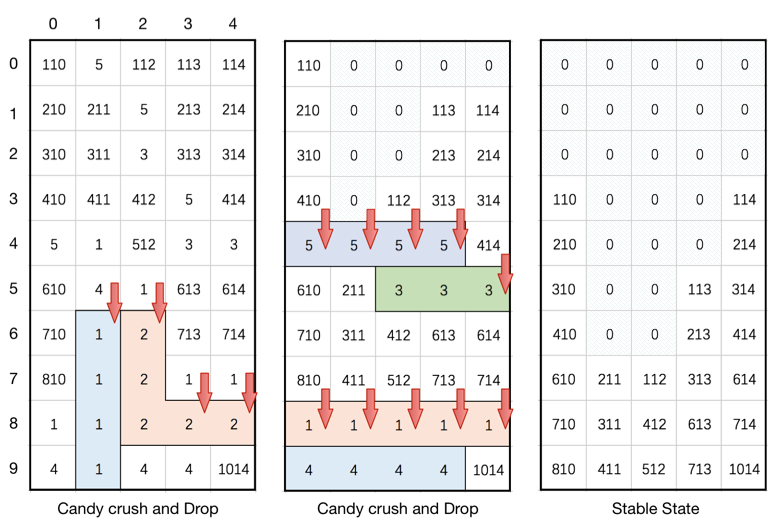
\includegraphics[width=300pt]{candy-crush-example-2.png}\\
\figcaption{candy crush}\label{fig:candy-crush-example}
\end{center}

\subsubsection{分析}

\subsubsection{代碼}
\begin{Code}
// LeetCode, Candy Crush
// 時間複雜度O(n),空間複雜度O(n)
class solution{
public:
    vector<vector<int>> candyCrush(vector<vector<int>>& board) {
        int M = board.size();
        int N = board[0].size();

        bool isNeedScan = true;
        while (isNeedScan)
        {
            // check row by row
            HandleRowByRow(board, M, N);
            // check col by col
            HandleColByCol(board, M, N);
            // dropping action
            isNeedScan = DoDropAction(board, M, N);
        }

        return board;
    }
private:
    void PrintBoard(vector<vector<int>>& board)
    {
        for (const auto& r : board)
        {
            for (const auto& c : r)
                cout << c << "\t";
            cout << endl;
        }
    }
    bool DoDropAction(vector<vector<int>>& board, int M, int N)
    {
        bool isDoDrop = false;
        // do dropping col by col
        for (int j = 0; j < N; j++)
        {
            int lowestNeg = M-1;
            while (lowestNeg >= 0 && board[lowestNeg][j] >= 0) lowestNeg--;
            if (lowestNeg >= 0) isDoDrop = true;

            // update next positive position
            int nextPositive = lowestNeg;
            while (nextPositive >= 0)
            {
                while (nextPositive >= 0 && board[nextPositive][j] < 0) nextPositive--;
                
                // move the data
                for (; nextPositive >= 0 && board[nextPositive][j] >= 0; nextPositive--)
                    board[lowestNeg--][j] = board[nextPositive][j];
            }
            for (; lowestNeg >= 0; lowestNeg--)
                board[lowestNeg][j] = 0;
        }
        
        return isDoDrop;
    }
    void HandleRowByRow(vector<vector<int>>& board, int M, int N)
    {
        for (int i = 0; i < M; i++)
        {
            for (int j = 0; j + 2 < N; j++)
            {
                int cur = abs(board[i][j]);
                bool found = false;
                while (j + 2 < N && cur == abs(board[i][j+1]) && cur == abs(board[i][j+2]))
                {
                    found = true;
                    board[i][j] = -cur;
                    j++;
                }
                if (found)
                {
                    board[i][j] = -cur;
                    board[i][++j] = -cur;
                }
            }
        }
    }
    void HandleColByCol(vector<vector<int>>& board, int M, int N)
    {
        for (int j = 0; j < N; j++)
        {
            for (int i = 0; i + 2 < M; i++)
            {
                int cur = abs(board[i][j]);
                bool found = false;
                while (i + 2 < M && cur == abs(board[i+1][j]) && cur == abs(board[i+2][j]))
                {
                    found = true;
                    board[i][j] = -cur;
                    i++;
                }
                if (found)
                {
                    board[i][j] = -cur;
                    board[++i][j] = -cur;
                }
            }
        }
    }
};
\end{Code}

\subsubsection{相關題目}
\begindot
\item Candy Crush II, 見 \S \ref{sec:candy-crush-ii}
\myenddot

\subsection{Intersection of Two Arrays}
\label{sec:intersection-of-two-arrays}


\subsubsection{描述}
Given two arrays, write a function to compute their intersection.

Example 1:
\begin{Code}
Input: nums1 = [1,2,2,1], nums2 = [2,2]
Output: [2]
\end{Code}

Example 2:
\begin{Code}
Input: nums1 = [4,9,5], nums2 = [9,4,9,8,4]
Output: [9,4]
\end{Code}

Note:
\begindot
\item Each element in the result must be unique.
\item The result can be in any order.
\myenddot

\subsubsection{分析}
1. Use std method\newline

2. Use hash map\newline

3. Sort then merge\newline

\subsubsection{代碼 - STD method}
\begin{Code}
// LeetCode
// 時間複雜度O(nlogn),空間複雜度O(n)
class solution{
public:
    vector<int> intersection(vector<int>& nums1, vector<int>& nums2) {
        // 先順序
        sort(nums1.begin(), nums1.end());
        sort(nums2.begin(), nums2.end());
        vector<int> result(nums1.size() + nums2.size());

        // 利用 std
        vector<int>::iterator it = set_intersection(nums1.begin(), nums1.end()
                                                    , nums2.begin(), nums2.end()
                                                    , result.begin());
        // 刪去多餘的空間
        result.resize(it - result.begin());
        // 刪去重覆
        result.erase(unique(result.begin(), result.end()), result.end());

        return result;
    }
};
\end{Code}

\subsubsection{代碼 - Hash map}
\begin{Code}
// LeetCode
// 時間複雜度O(n),空間複雜度O(n)
class solution{
public:
    vector<int> intersection(vector<int>& nums1, vector<int>& nums2) {
        // 使用 hash map
        unordered_set<int> map1(nums1.begin(), nums1.end());
        unordered_set<int> map2(nums2.begin(), nums2.end());
        vector<int> result; result.reserve(map1.size() + map2.size());

        for (const auto& e1 : map1) {
            // 在兩個 hash map 中出現,便是答案
            auto it = map2.find(e1);
            if (it != map2.end()) result.push_back(e1);
        }

        return result;
    }
};
\end{Code}

\subsubsection{代碼 - Merge vector}
\begin{Code}
// LeetCode
// 時間複雜度O(nlogn),空間複雜度O(n)
class solution{
public:
    vector<int> intersection(vector<int>& nums1, vector<int>& nums2) {
        // 先順序
        sort(nums1.begin(), nums1.end());
        sort(nums2.begin(), nums2.end());
        vector<int> result; result.reserve(nums1.size() + nums2.size());

        // merge 兩支 vector
        for (int p1 = 0, p2 = 0; p1 < nums1.size() && p2 < nums2.size()) {
            if (nums1[p1] < nums2[p2])
                p1++;
            else if (nums1[p1] > nums2[p2])
                p2++;
            else {
                result.push_back(nums1[p1]);
                p1++;
                p2++;
            }
        }
        // 除去重覆
        result.erase(unique(result.begin(), result.end()), result.end());

        return result;
    }
};
\end{Code}


\subsection{Find the Duplicate Number}
\label{sec:find-the-duplicate-number}


\subsubsection{描述}
Given an array nums containing n + 1 integers where each integer is between 1 and n (inclusive), prove that at least one duplicate number must exist. Assume that there is only one duplicate number, find the duplicate one.


Example 1:
\begin{Code}
Input: [1,3,4,2,2]
Output: 2
\end{Code}

Example 2:
\begin{Code}
Input: [3,1,3,4,2]
Output: 3
\end{Code}


\subsubsection{分析}
Nil

\subsubsection{代碼 - Cycle - bucket sort}
\begin{Code}
// LeetCode
// 時間複雜度O(nlogn),空間複雜度O(n)
class solution{
public:
    int findDuplicate(vector<int>& nums) {
        // 這個跟 cycle linked list 差不多
        // 重覆的 element 會形成 cycle
        int fast = nums[0];
        int slow = nums[0];

        do {
            fast = nums[nums[fast]];
            slow = nums[slow];
        } while (fast != slow);

        int slow2 = nums[0];
        while (slow2 != slow) {
            slow2 = nums[slow2];
            slow = nums[slow];
        }

        return slow2;
    }
};
\end{Code}


\subsection{Find K-th Smallest Pair Distance}
\label{sec:kth-smallest-pair-distance}


\subsubsection{描述}
Given an integer array, return the k-th smallest distance among all the pairs. The distance of a pair (A, B) is defined as the absolute difference between A and B.

Example 1:
\begin{Code}
Input:
nums = [1,3,1]
k = 1
Output: 0 
Explanation:
Here are all the pairs:
(1,3) -> 2
(1,1) -> 0
(3,1) -> 2
Then the 1st smallest distance pair is (1,1), and its distance is 0.
\end{Code}


\begindot
\item 2 <= len(nums) <= 10000.
\item 0 <= nums[i] < 1000000.
\item 1 <= k <= len(nums) * (len(nums) - 1) / 2.
\myenddot

\subsubsection{分析}
估一個 distance 值,數一數有多少個 distance 值係細過此一估值。然後以二分法原則去調整估值的大細。

\subsubsection{代碼}
\begin{Code}
// LeetCode
// 時間複雜度O(nlogn),空間複雜度O(n)
class Solution {
public:
    int smallestDistancePair(vector<int>& nums, int k) {
        if (nums.size() == 0) return 0;
        sort(nums.begin(), nums.end());

        int lo = 0;
        int hi = nums[nums.size() - 1] - nums[0];
        while (lo < hi) {
            int mi = lo + (hi - lo) / 2; // 得出估值
            int count = 0, left = 0;
            for (int right = 0; right < nums.size(); ++right) {
                while (nums[right] - nums[left] > mi) left++;
                count += right - left;
            }
            //count = number of pairs with distance <= mi
            if (count >= k) hi = mi; // 二分法來調整估值大細
            else lo = mi + 1;
        }
        return lo;
    }
};
\end{Code}

\subsection{Find Pivot Index}
\label{sec:find-pivot-index}

\subsubsection{描述}
Given an array of integers nums, write a method that returns the "pivot" index of this array.

We define the pivot index as the index where the sum of all the numbers to the left of the index is equal to the sum of all the numbers to the right of the index.

If no such index exists, we should return -1. If there are multiple pivot indexes, you should return the left-most pivot index.

Example 1:
\begin{Code}
Input: nums = [1,7,3,6,5,6]
Output: 3
Explanation:
The sum of the numbers to the left of index 3 (nums[3] = 6) is equal to the sum of numbers to the right of index 3.
Also, 3 is the first index where this occurs.
\end{Code}

Example 2:
\begin{Code}
Input: nums = [1,2,3]
Output: -1
Explanation:
There is no index that satisfies the conditions in the problem statement.
\end{Code}

\subsubsection{分析}
先計算總數,往右走,每走一步都會跟左邊總加值對比。

\subsubsection{代碼}
\begin{Code}
// LeetCode
// 時間複雜度O(),空間複雜度O()
class Solution {
public:
    int pivotIndex(vector<int>& nums) {
        int sum = 0, leftsum = 0;
        for (int x: nums) sum += x;
        for (int i = 0; i < nums.size(); ++i) {
            if (leftsum == sum - leftsum - nums[i]) return i;
            leftsum += nums[i];
        }
        return -1;
    }
};
\end{Code}


\subsection{Largest Number At Least Twice of Others}
\label{sec:largest-number-at-least-twice-of-others}

\subsubsection{描述}
In a given integer array nums, there is always exactly one largest element.

Find whether the largest element in the array is at least twice as much as every other number in the array.

If it is, return the index of the largest element, otherwise return -1.

Example 1:
\begin{Code}
Input: nums = [3, 6, 1, 0]
Output: 1
Explanation: 6 is the largest integer, and for every other number in the array x,
6 is more than twice as big as x.  The index of value 6 is 1, so we return 1.
\end{Code}

Example 2:
\begin{Code}
Input: nums = [1, 2, 3, 4]
Output: -1
Explanation: 4 isn't at least as big as twice the value of 3, so we return -1.
\end{Code}

Note:
\begindot
\item nums will have a length in the range [1, 50].
\item Every nums[i] will be an integer in the range [0, 99].
\myenddot

\subsubsection{分析}
first pass 先求得最大值,second pass 找尋第二大的一倍數值,若過大,回值 -1

\subsubsection{代碼}
\begin{Code}
// LeetCode
// 時間複雜度O(),空間複雜度O()
class Solution {
public:
    int dominantIndex(vector<int>& nums) {
        int N = nums.size();
        if (N == 0) return -1;

        int firstMax = INT_MIN;
        int maxIndex = -1;

        for (int i = 0; i < N; i++) {
            if (nums[i] > firstMax) {
                firstMax = nums[i];
                maxIndex = i;
            }
        }
        for (int i = 0; i < N; i++) {
            if (firstMax > nums[i])
                if (firstMax < 2 * nums[i]) return -1;
        }

        return maxIndex;
    }
};
\end{Code}

\subsection{Array Partition I}
\label{sec:array-partition-i}

\subsubsection{描述}
Given an array of 2n integers, your task is to group these integers into n pairs of integer, say (a1, b1), (a2, b2), ..., (an, bn) which makes sum of min(ai, bi) for all i from 1 to n as large as possible.

Example 1:
\begin{Code}
Input: [1,4,3,2]

Output: 4
Explanation: n is 2, and the maximum sum of pairs is 4 = min(1, 2) + min(3, 4).
\end{Code}

Note:
\begindot
\item n is a positive integer, which is in the range of [1, 10000].
\item All the integers in the array will be in the range of [-10000, 10000].
\myenddot

\subsubsection{分析}
Nil

\subsubsection{代碼}
\begin{Code}
// LeetCode
// 時間複雜度O(n),空間複雜度O(n)
class Solution {
public:
    int arrayPairSum(vector<int>& nums) {
        vector<int> arr(20001, 0);
        int shift = 10000;
        for (const int& num : nums)
            arr[num + shift]++;
        int d = 0, sum = 0;
        for (int i = -10000; i <= 10000; i++)
        {
            sum += (arr[i + shift] + 1 - d) / 2 * i;
            d = (2 + arr[i + shift] - d) % 2; // 在前邊加 2,用來防止負數的出現。
        }
        return sum;
    }
};
\end{Code}

\subsubsection{代碼}
\begin{Code}
// LeetCode
// 時間複雜度O(nlogn),空間複雜度O(1)
class Solution {
public:
    int arrayPairSum(vector<int>& nums) {
        sort(nums.begin(), nums.end());
        int sum = 0;
        for (int i = 0; i < nums.size(); i += 2)
            sum += nums[i];

        return sum;
    }
};
\end{Code}


\subsection{Rotate Array}
\label{sec:rotate-array}

\subsubsection{描述}
Given an array, rotate the array to the right by k steps, where k is non-negative.

Example 1:
\begin{Code}
Input: nums = [1,2,3,4,5,6,7], k = 3
Output: [5,6,7,1,2,3,4]
Explanation:
rotate 1 steps to the right: [7,1,2,3,4,5,6]
rotate 2 steps to the right: [6,7,1,2,3,4,5]
rotate 3 steps to the right: [5,6,7,1,2,3,4]
\end{Code}

Example 2:
\begin{Code}
Input: nums = [-1,-100,3,99], k = 2
Output: [3,99,-1,-100]
Explanation: 
rotate 1 steps to the right: [99,-1,-100,3]
rotate 2 steps to the right: [3,99,-1,-100]
\end{Code}

\subsubsection{額外的空間}
\begin{Code}
// LeetCode
// 時間複雜度O(n),空間複雜度O(n)
class Solution {
public:
    void rotate(vector<int>& nums, int k) {
        vector<int> a(nums.size());

        for (int i = 0; i < nums.size(); i++)
            a[(i + k) % nums.size()] = nums[i];

        nums = a;
    }
};
\end{Code}

\subsubsection{循環取代法}
\begin{center}
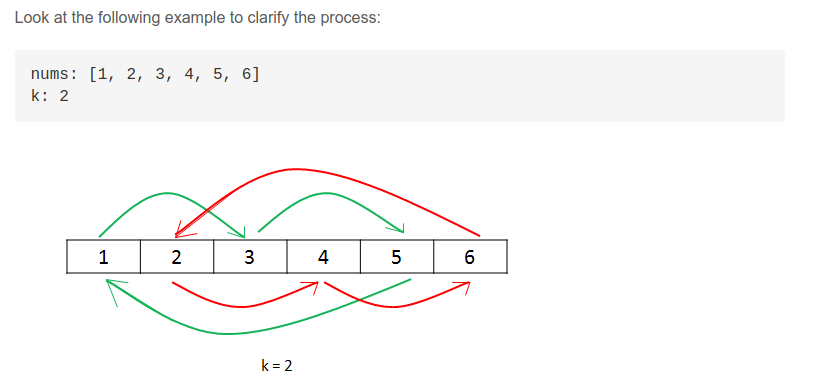
\includegraphics[width=300pt]{cyclic-replacements.png}\\
\figcaption{cyclic replacements}\label{fig:cyclic-replacements}
\end{center}

\begin{Code}
// LeetCode
// 時間複雜度O(n),空間複雜度O(1)
class Solution {
public:
    void rotate(vector<int>& nums, int k) {
        k = k % nums.size();
        int count = 0;
        for (int start = 0; count < nums.size(); start++) {
            int current = start;
            int prev = nums[start];
            do {
                int next = (current + k) % nums.size();
                int temp = nums[next];
                nums[next] = prev;
                prev = temp;
                current = next;
                count++;
            } while (start != current);
        }
    }
};
\end{Code}

\subsubsection{reverse}
\begin{Code}
Original List                   : 1 2 3 4 5 6 7
After reversing all numbers     : 7 6 5 4 3 2 1
After reversing first k numbers : 5 6 7 4 3 2 1
After revering last n-k numbers : 5 6 7 1 2 3 4 --> Result
\end{Code}

\begin{Code}
// LeetCode
// 時間複雜度O(n),空間複雜度O(1)
class Solution {
public:
    void rotate(vector<int>& nums, int k) {
        k %= nums.size();
        reverse(nums, 0, nums.size() - 1);
        reverse(nums, 0, k - 1);
        reverse(nums, k, nums.size() - 1);
    }
private:
    void reverse(vector<int>& nums, int start, int end) {
        while (start < end) {
            int temp = nums[start];
            nums[start] = nums[end];
            nums[end] = temp;
            start++;
            end--;
        }
    }
};
\end{Code}


\subsection{Reverse Words in a String}
\label{sec:reverse-words-in-a-string}

\subsubsection{描述}
Given an input string, reverse the string word by word.

Example 1:
\begin{Code}
Input: "the sky is blue"
Output: "blue is sky the"
\end{Code}

Example 2:
\begin{Code}
Input: "  hello world!  "
Output: "world! hello"
Explanation: Your reversed string should not contain leading or trailing spaces.
\end{Code}

Example 3:
\begin{Code}
Input: "a good   example"
Output: "example good a"
Explanation: You need to reduce multiple spaces between two words to a single space in the reversed string.
\end{Code}

Note:
\begindot
\item A word is defined as a sequence of non-space characters.
\item Input string may contain leading or trailing spaces. However,
      your reversed string should not contain leading or trailing spaces.
\item You need to reduce multiple spaces between two words to a single space in the reversed string.
\myenddot

\subsubsection{分析}
Reverse

\subsubsection{代碼}
\begin{Code}
// LeetCode
// 時間複雜度O(n),空間複雜度O(1)
class Solution {
public:
    string reverseWords(string s) {
        if (s.size() == 0) return s;
        // 整段 reverse
        MyReverse(s.begin(), s.end());
        // 每個字 reverse
        auto cur = s.begin();
        auto next = cur;

        while (next < s.end())
        {
            // 尋找字的開端
            cur = find_if(cur, s.end(), [&](const char& c) { return (c != ' '); });
            // 尋找空白的開端
            next = find_if(cur, s.end(), [&](const char& c) { return (c == ' '); });

            MyReverse(cur, next);

            cur = next;
        }

        // 對應的 std 方法
        // s.erase(s.find_last_not_of(' ')+1); // 移除領先空格
        // s.erase(0, s.find_first_not_of(' ')); // 移除尾隨空格
        s.erase(InPlaceRemoveSpace(s.begin(), s.end()), s.end());
        return s;
    }
private:
    template <class RandIT>
        RandIT InPlaceRemoveSpace(RandIT first, RandIT last)
    {
        bool isFirst = true;
        // 移除領先空格,尾隨空格,中間多餘空格
        auto cur = first;
        while (first < last)
        {
            // 找尋下一個字
            first = find_if(first, last, [&](const char& c) { return (c != ' '); });
            if (first >= last) break;

            if (!isFirst) *cur++ = ' '; // 只有當不是第一個文字,會加入空格
            while (first < last && *first != ' ') *cur++ = *first++; // 補上文字,直至空格出現
            if (first >= last) break;
            isFirst = false;
        }

        return cur;
    }
    template <class RandIT>
        void MyReverse(RandIT first, RandIT last)
    {
        last--;
        while (first < last)
        {
            // 進行 swap
            auto tmp = *last;
            *last-- = *first;
            *first++ = tmp;
        }
    }
};
\end{Code}

\subsection{Happy Number}
\label{sec:happy-number}

\subsubsection{描述}
Write an algorithm to determine if a number n is "happy".

A happy number is a number defined by the following process: Starting with any positive integer, replace the number by the sum of the squares of its digits, and repeat the process until the number equals 1 (where it will stay), or it loops endlessly in a cycle which does not include 1. Those numbers for which this process ends in 1 are happy numbers.

Return True if n is a happy number, and False if not.

Example:
\begin{Code}
Input: 19
Output: true
Explanation: 
1^2 + 9^2 = 82
8^2 + 2^2 = 68
6^2 + 8^2 = 100
1^2 + 0^2 + 0^2 = 1
\end{Code}

\subsubsection{利用循環特性}
\begin{center}
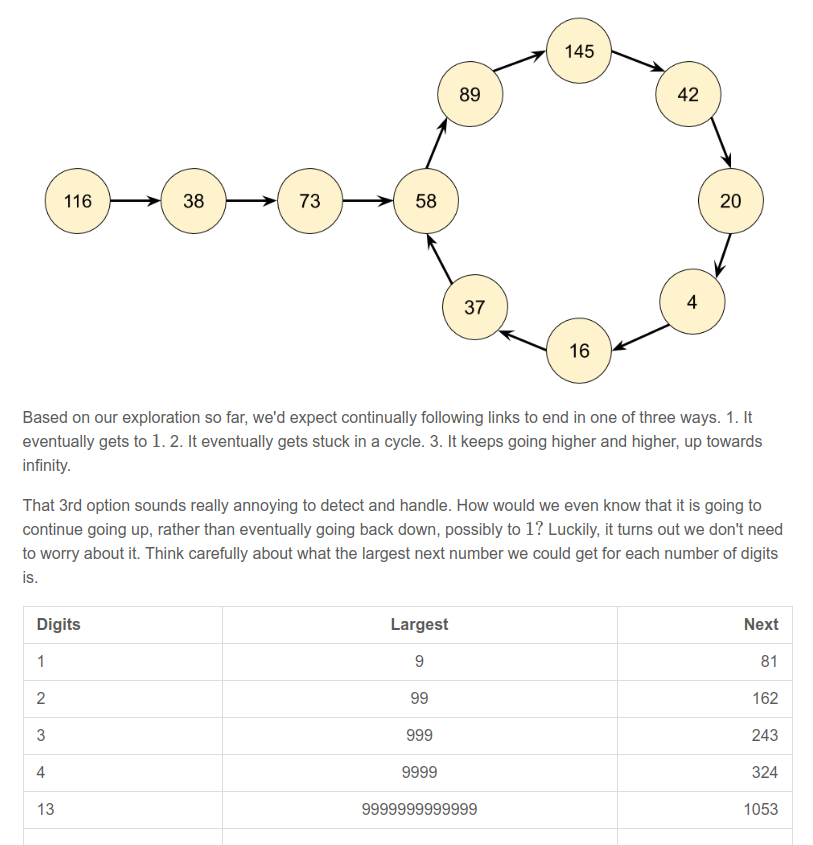
\includegraphics[width=300pt]{happy-number-001.png}\\
\figcaption{Why have loop}\label{fig:happy-number-001}
\end{center}

\begin{Code}
// LeetCode
// 時間複雜度O(n),空間複雜度O(n)
class Solution {
public:
    bool isHappy(int n) {
        unordered_set<int> seen;

        // 由例子中可以看到,若果計不到 1 ,便會重覆
        // 並且不會愈計愈大,所以可以用這個方法
        while (n != 1 && seen.find(n) == seen.end())
        {
            seen.insert(n);
            n = GetNext(n);
        }

        return n == 1;
    }
private:
    int GetNext(int n)
    {
        int result = 0;
        while (n)
        {
            int d = n % 10;
            result += d * d;
            n /= 10;
        }

        return result;
    }
};
\end{Code}

\subsubsection{快慢雙指針法}
\begin{Code}
// LeetCode
// 時間複雜度O(logN),空間複雜度O(1)
class Solution {
public:
    bool isHappy(int n) {
        int slow = n;
        int fast = GetNext(slow);

        while (fast != 1 && fast != slow)
        {
            slow = GetNext(slow);
            fast = GetNext(GetNext(fast));
        }

        return fast == 1;
    }
private:
    int GetNext(int n)
    {
        int result = 0;
        while (n)
        {
            int d = n % 10;
            result += d * d;
            n /= 10;
        }

        return result;
    }
};
\end{Code}

\subsubsection{數學規則}
\begin{Code}
// LeetCode
// 時間複雜度O(logN),空間複雜度O(1)
class Solution {
public:
    bool isHappy(int n) {
        // 通過觀察,只有以下路徑會循環
        // 4 -> 16 -> 37 -> 58 -> 89 -> 145 -> 42 -> 20 -> 4
        while (n != 1 && n != 4)
            n = GetNext(n);

        return n == 1;
    }
private:
    int GetNext(int n)
    {
        int result = 0;
        while (n)
        {
            int d = n % 10;
            result += d * d;
            n /= 10;
        }

        return result;
    }
};
\end{Code}

\subsection{Isomorphic Strings}
\label{sec:isomorphic-strings}

\subsubsection{描述}
Given two strings s and t, determine if they are isomorphic.

Two strings are isomorphic if the characters in s can be replaced to get t.

All occurrences of a character must be replaced with another character while preserving the order of characters. No two characters may map to the same character but a character may map to itself.

Example 1:
\begin{Code}
Input: s = "egg", t = "add"
Output: true
\end{Code}

Example 2:
\begin{Code}
Input: s = "foo", t = "bar"
Output: false
\end{Code}

Example 3:
\begin{Code}
Input: s = "paper", t = "title"
Output: true
\end{Code}

\subsubsection{字母 hash}
\begin{Code}
// LeetCode
// 時間複雜度O(n),空間複雜度O(n)
class Solution {
public:
    bool isIsomorphic(string s, string t) {
        vector<char> v1(256, 0);
        vector<char> v2(256, 0);

        for (size_t i = 0; i < s.size(); i++)
        {
            if (v1[s[i]] != 0 && v1[s[i]] != t[i]) return false;
            if (v2[t[i]] != 0 && v2[t[i]] != s[i]) return false;

            v1[s[i]] = t[i];
            v2[t[i]] = s[i];
        }

        return true;
    }
};
\end{Code}

\subsection{Group Shifted Strings}
\label{sec:group-shifted-strings}

\subsubsection{描述}
Given a string, we can "shift" each of its letter to its successive letter, for example: "abc" -> "bcd". We can keep "shifting" which forms the sequence:

\begin{Code}
"abc" -> "bcd" -> ... -> "xyz"
\end{Code}

Given a list of non-empty strings which contains only lowercase alphabets, group all strings that belong to the same shifting sequence.

Example:
\begin{Code}
Input: ["abc", "bcd", "acef", "xyz", "az", "ba", "a", "z"],
Output: 
[
  ["abc","bcd","xyz"],
  ["az","ba"],
  ["acef"],
  ["a","z"]
]
\end{Code}

\subsubsection{暴力 shift}
\begin{Code}
// LeetCode
// 時間複雜度O(n),空間複雜度O(n)
class Solution {
public:
    vector<vector<string>> groupStrings(vector<string>& strings) {
        unordered_map<string, vector<string>> hashMap;
        for(auto &str : strings) {
            string temp = str;
            convertStringToKey(temp);
            hashMap[temp].push_back(str);
        }

        vector<vector<string>> answer;
        for(auto it = hashMap.begin(); it != hashMap.end(); ++it) {
            answer.push_back(it->second);
        }
        return answer;
    }
private:
    void convertStringToKey(string &str) {
        while(str[0] != 'a') {
            for(int i = 0; i < str.size(); ++i) {
                str[i] += 1;
                if(str[i] > 'z') {
                    str[i] = 'a';
                }
            }
        }
    }
};
\end{Code}

\subsubsection{Counting shift}
\begin{Code}
// LeetCode
// 時間複雜度O(n),空間複雜度O(n)
class Solution {
public:
    vector<vector<string>> groupStrings(vector<string>& strings) {
        unordered_map<string, vector<string>> hashMap;
        for(auto &str : strings) {
            string temp = str;
            convertStringToKey(temp);
            hashMap[temp].push_back(str);
        }

        vector<vector<string>> answer;
        for(auto it = hashMap.begin(); it != hashMap.end(); ++it) {
            answer.push_back(it->second);
        }
        return answer;
    }
private:
    void convertStringToKey(string &str) {
        if (str.size() == 0) return;

        if (str[0] != 'a')
        {
            int diffFromA = str[0] - 'a';

            for (size_t i = 0; i < str.size(); ++i)
            {
                if ((str[i] - 'a') < diffFromA)
                    str[i] = (26 + str[i] - diffFromA);
                else
                    str[i] = str[i] - diffFromA;
            }
        }
    }
};
\end{Code}

\chapter{鏈表}

\section{單鏈表} %%%%%%%%%%%%%%%%%%%%%%%%%%%%%%

單鏈表節點的定義如下:
\begin{Code}
// 單鏈表節點
struct ListNode {
    int val;
    ListNode *next;
    ListNode(int x) : val(x), next(nullptr) { }
};
\end{Code}


\subsection{Add Two Numbers}
\label{sec:add-two-numbers}


\subsubsection{描述}
You are given two linked lists representing two non-negative numbers. The digits are stored in reverse order and each of their nodes contain a single digit. Add the two numbers and return it as a linked list.

Input: {\small \fontspec{Latin Modern Mono} (2 -> 4 -> 3) + (5 -> 6 -> 4)}

Output: {\small \fontspec{Latin Modern Mono} 7 -> 0 -> 8}


\subsubsection{分析}
跟Add Binary(見 \S \ref{sec:add-binary})很類似


\subsubsection{代碼}
\begin{Code}
// LeetCode, Add Two Numbers
// 跟Add Binary 很類似
// 時間複雜度O(m+n),空間複雜度O(1)
class Solution {
public:
    ListNode *addTwoNumbers(ListNode *l1, ListNode *l2) {
        ListNode dummy(-1); // 頭節點
        int carry = 0;
        ListNode *prev = &dummy;
        for (ListNode *pa = l1, *pb = l2;
             pa != nullptr || pb != nullptr;
             pa = pa == nullptr ? nullptr : pa->next,
             pb = pb == nullptr ? nullptr : pb->next,
             prev = prev->next) {
            const int ai = pa == nullptr ? 0 : pa->val;
            const int bi = pb == nullptr ? 0 : pb->val;
            const int value = (ai + bi + carry) % 10;
            carry = (ai + bi + carry) / 10;
            prev->next = new ListNode(value); // 尾插法
        }
        if (carry > 0)
            prev->next = new ListNode(carry);
        return dummy.next;
    }
};
\end{Code}


\subsubsection{相關題目}

\begindot
\item Add Binary, 見 \S \ref{sec:add-binary}
\myenddot


\subsection{Reverse Linked List II}
\label{sec:reverse-linked-list-ii}


\subsubsection{描述}
Reverse a linked list from position $m$ to $n$. Do it in-place and in one-pass.

For example:
Given \code{1->2->3->4->5->nullptr}, $m$ = 2 and $n$ = 4,

return \code{1->4->3->2->5->nullptr}.

Note:
Given m, n satisfy the following condition:
$1 \leq m \leq  n \leq $ length of list.


\subsubsection{分析}
這題非常繁瑣,有很多邊界檢查,15分鐘內做到bug free很有難度!


\subsubsection{代碼}
\begin{Code}
// LeetCode, Reverse Linked List II
// 迭代版,時間複雜度O(n),空間複雜度O(1)
class Solution {
public:
    ListNode *reverseBetween(ListNode *head, int m, int n) {
        ListNode dummy(-1);
        dummy.next = head;

        ListNode *prev = &dummy;
        for (int i = 0; i < m-1; ++i)
            prev = prev->next;
        ListNode* const head2 = prev;

        prev = head2->next;
        ListNode *cur = prev->next;
        for (int i = m; i < n; ++i) {
            prev->next = cur->next;
            cur->next = head2->next;
            head2->next = cur;  // 頭插法
            cur = prev->next;
        }

        return dummy.next;
    }
};
\end{Code}


\subsubsection{相關題目}

\begindot
\item 無
\myenddot


\subsection{Partition List}
\label{sec:partition-list}


\subsubsection{描述}
Given a linked list and a value $x$, partition it such that all nodes less than $x$ come before nodes greater than or equal to $x$.

You should preserve the original relative order of the nodes in each of the two partitions.

For example,
Given \code{1->4->3->2->5->2} and \code{x = 3}, return \code{1->2->2->3->4->5}.


\subsubsection{分析}
無


\subsubsection{代碼}
\begin{Code}
// LeetCode, Partition List
// 時間複雜度O(n),空間複雜度O(1)
class Solution {
public:
    ListNode* partition(ListNode* head, int x) {
        ListNode left_dummy(-1); // 頭結點
        ListNode right_dummy(-1); // 頭結點

        auto left_cur = &left_dummy;
        auto right_cur = &right_dummy;

        for (ListNode *cur = head; cur; cur = cur->next) {
            if (cur->val < x) {
                left_cur->next = cur;
                left_cur = cur;
            } else {
                right_cur->next = cur;
                right_cur = cur;
            }
        }

        left_cur->next = right_dummy.next;
        right_cur->next = nullptr;

        return left_dummy.next;
    }
};
\end{Code}


\subsubsection{相關題目}

\begindot
\item 無
\myenddot


\subsection{Remove Duplicates from Sorted List}
\label{sec:remove-duplicates-from-sorted-list}


\subsubsection{描述}
Given a sorted linked list, delete all duplicates such that each element appear only once.

For example,

Given \code{1->1->2}, return \code{1->2}.

Given \code{1->1->2->3->3}, return \code{1->2->3}.


\subsubsection{分析}
無


\subsubsection{遞歸版}
\begin{Code}
// LeetCode, Remove Duplicates from Sorted List
// 遞歸版,時間複雜度O(n),空間複雜度O(1)
class Solution {
public:
    ListNode *deleteDuplicates(ListNode *head) {
        if (!head) return head;
        ListNode dummy(head->val + 1); // 值只要跟head不同即可
        dummy.next = head;

        recur(&dummy, head);
        return dummy.next;
    }
private:
    static void recur(ListNode *prev, ListNode *cur) {
        if (cur == nullptr) return;

        if (prev->val == cur->val) { // 刪除head
            prev->next = cur->next;
            delete cur;
            recur(prev, prev->next);
        } else {
            recur(prev->next, cur->next);
        }
    }
};
\end{Code}


\subsubsection{迭代版}
\begin{Code}
// LeetCode, Remove Duplicates from Sorted List
// 迭代版,時間複雜度O(n),空間複雜度O(1)
class Solution {
public:
    ListNode *deleteDuplicates(ListNode *head) {
        if (head == nullptr) return nullptr;

        for (ListNode *prev = head, *cur = head->next; cur; cur = prev->next) {
            if (prev->val == cur->val) {
                prev->next = cur->next;
                delete cur;
            } else {
                prev = cur;
            }
        }
        return head;
    }
};
\end{Code}


\subsubsection{相關題目}

\begindot
\item Remove Duplicates from Sorted List II,見 \S \ref{sec:remove-duplicates-from-sorted-list-ii}
\myenddot


\subsection{Remove Duplicates from Sorted List II}
\label{sec:remove-duplicates-from-sorted-list-ii}


\subsubsection{描述}
Given a sorted linked list, delete all nodes that have duplicate numbers, leaving only distinct numbers from the original list.

For example,

Given \code{1->2->3->3->4->4->5}, return \code{1->2->5}.

Given \code{1->1->1->2->3}, return \code{2->3}.


\subsubsection{分析}
無


\subsubsection{遞歸版}
\begin{Code}
// LeetCode, Remove Duplicates from Sorted List II
// 遞歸版,時間複雜度O(n),空間複雜度O(1)
class Solution {
public:
    ListNode *deleteDuplicates(ListNode *head) {
        if (!head || !head->next) return head;

        ListNode *p = head->next;
        if (head->val == p->val) {
            while (p && head->val == p->val) {
                ListNode *tmp = p;
                p = p->next;
                delete tmp;
            }
            delete head;
            return deleteDuplicates(p);
        } else {
            head->next = deleteDuplicates(head->next);
            return head;
        }
    }
};
\end{Code}


\subsubsection{迭代版}
\begin{Code}
// LeetCode, Remove Duplicates from Sorted List II
// 迭代版,時間複雜度O(n),空間複雜度O(1)
class Solution {
public:
    ListNode *deleteDuplicates(ListNode *head) {
        if (head == nullptr) return head;

        ListNode dummy(INT_MIN); // 頭結點
        dummy.next = head;
        ListNode *prev = &dummy, *cur = head;
        while (cur != nullptr) {
            bool duplicated = false;
            while (cur->next != nullptr && cur->val == cur->next->val) {
                duplicated = true;
                ListNode *temp = cur;
                cur = cur->next;
                delete temp;
            }
            if (duplicated) { // 刪除重複的最後一個元素
                ListNode *temp = cur;
                cur = cur->next;
                delete temp;
                continue;
            }
            prev->next = cur;
            prev = prev->next;
            cur = cur->next;
        }
        prev->next = cur;
        return dummy.next;
    }
};
\end{Code}


\subsubsection{迭代版}
\begin{Code}
// LeetCode, Remove Duplicates from Sorted List II
// 迭代版,時間複雜度O(n),空間複雜度O(1)
class Solution {
public:
    ListNode *deleteDuplicates(ListNode *head) {
        if (head == nullptr) return head;

        ListNode dummy(INT_MIN); dummy.next = head;
        ListNode *prev = &dummy;
        ListNode *cur = head;
        ListNode *next = cur != nullptr ? cur->next : nullptr;

        while (next != nullptr) {
            bool duplicated = false;
            while (next && cur->val == next->val) {
                duplicated = true;
                prev->next = next;
                delete cur;
                cur = next;
                next = cur != nullptr ? cur->next : nullptr;
            }
            if (duplicated) {
                prev->next = next;
                delete cur;
            }
            else
                prev = cur;
            cur = next;
            next = cur != nullptr ? cur->next : nullptr;
        }
        return dummy.next;
    }
};


\end{Code}
\subsubsection{相關題目}

\begindot
\item Remove Duplicates from Sorted List,見 \S \ref{sec:remove-duplicates-from-sorted-list}
\myenddot


\subsection{Rotate List}
\label{sec:rotate-list}


\subsubsection{描述}
Given a list, rotate the list to the right by $k$ places, where $k$ is non-negative.

For example:
Given \code{1->2->3->4->5->nullptr} and \code{k = 2}, return \code{4->5->1->2->3->nullptr}.


\subsubsection{分析}
先遍歷一遍,得出鏈表長度$len$,注意$k$可能大於$len$,因此令$k \%= len$。將尾節點next指針指向首節點,形成一個環,接着往後跑$len-k$步,從這裏斷開,就是要求的結果了。


\subsubsection{代碼}
\begin{Code}
// LeetCode, Remove Rotate List
// 時間複雜度O(n),空間複雜度O(1)
class Solution {
public:
    ListNode *rotateRight(ListNode *head, int k) {
        if (head == nullptr || k == 0) return head;

        int len = 1;
        ListNode* p = head;
        while (p->next) { // 求長度
            len++;
            p = p->next;
        }
        k = len - k % len;

        p->next = head; // 首尾相連
        for(int step = 0; step < k; step++) {
            p = p->next;  //接着往後跑
        }
        head = p->next; // 新的首節點
        p->next = nullptr; // 斷開環
        return head;
    }
};
\end{Code}


\subsubsection{相關題目}

\begindot
\item 無
\myenddot

\subsection{Rotate List II}
\label{sec:rotate-list-ii}


\subsubsection{描述}
Given a list, rotate the list to the left by $k$ places, where $k$ is non-negative.

For example:
Given \code{1->2->3->4->5->nullptr} and \code{k = 2}, return \code{4->5->1->2->3->nullptr}.


\subsubsection{分析}
先遍歷一遍,得出鏈表長度$len$,注意$k$可能大於$len$,因此令$k \%= len$。將尾節點next指針指向首節點,形成一個環,接着往後跑$len-k$步,從這裏斷開,就是要求的結果了。


\subsubsection{代碼}
\begin{Code}
// LeetCode, Remove Rotate List
// 時間複雜度O(n),空間複雜度O(1)
class Solution {
public:
    ListNode *rotateRight(ListNode *head, int k) {
        if (head == nullptr || k == 0) return head;

        int len = 1;
        ListNode* p = head;
        while (p->next) { // 求長度
            len++;
            p = p->next;
        }
        k = k % len; // This is the only difference

        p->next = head; // 首尾相連
        for(int step = 0; step < k; step++) {
            p = p->next;  //接着往後跑
        }
        head = p->next; // 新的首節點
        p->next = nullptr; // 斷開環
        return head;
    }
};
\end{Code}


\subsubsection{相關題目}

\begindot
\item 無
\myenddot


\subsection{Remove Nth Node From End of List}
\label{sec:remove-nth-node-from-end-of-list}


\subsubsection{描述}
Given a linked list, remove the $n^{th}$ node from the end of list and return its head.

For example, Given linked list: \code{1->2->3->4->5}, and $n$ = 2.

After removing the second node from the end, the linked list becomes \code{1->2->3->5}.

Note:
\begindot
\item Given $n$ will always be valid.
\item Try to do this in one pass.
\myenddot


\subsubsection{分析}
設兩個指針$p,q$,讓$q$先走$n$步,然後$p$和$q$一起走,直到$q$走到尾節點,刪除\fn{p->next}即可。


\subsubsection{代碼}
\begin{Code}
// LeetCode, Remove Nth Node From End of List
// 時間複雜度O(n),空間複雜度O(1)
class Solution {
public:
    ListNode *removeNthFromEnd(ListNode *head, int n) {
        ListNode dummy{-1, head};
        ListNode *p = &dummy, *q = &dummy;

        for (int i = 0; i < n; i++)  // q先走n步
            q = q->next;

        while(q->next) { // 一起走
            p = p->next;
            q = q->next;
        }
        ListNode *tmp = p->next;
        p->next = p->next->next;
        delete tmp;
        return dummy.next;
    }
};
\end{Code}


\subsubsection{相關題目}

\begindot
\item 無
\myenddot


\subsection{Swap Nodes in Pairs}
\label{sec:swap-nodes-in-pairs}


\subsubsection{描述}
Given a linked list, swap every two adjacent nodes and return its head.

For example,
Given \code{1->2->3->4}, you should return the list as \code{2->1->4->3}.

Your algorithm should use only constant space. You may \emph{not} modify the values in the list, only nodes itself can be changed.


\subsubsection{分析}
無


\subsubsection{代碼}
\begin{Code}
// LeetCode, Swap Nodes in Pairs
// 時間複雜度O(n),空間複雜度O(1)
class Solution {
public:
    ListNode *swapPairs(ListNode *head) {
        if (head == nullptr || head->next == nullptr) return head;
        ListNode dummy(-1);
        dummy.next = head;

        for(ListNode *prev = &dummy, *cur = prev->next, *next = cur->next;
                next;
                prev = cur, cur = cur->next, next = cur ? cur->next: nullptr) {
            prev->next = next;
            cur->next = next->next;
            next->next = cur;
        }
        return dummy.next;
    }
};
\end{Code}

下面這種寫法更簡潔,但題目規定了不允許這樣做。
\begin{Code}
// LeetCode, Swap Nodes in Pairs
// 時間複雜度O(n),空間複雜度O(1)
class Solution {
public:
    ListNode* swapPairs(ListNode* head) {
        ListNode* p = head;

        while (p && p->next) {
            swap(p->val, p->next->val);
            p = p->next->next;
        }

        return head;
    }
};
\end{Code}

\subsubsection{相關題目}

\begindot
\item Reverse Nodes in k-Group, 見 \S \ref{sec:reverse-nodes-in-k-group}
\myenddot


\subsection{Reverse Nodes in k-Group}
\label{sec:reverse-nodes-in-k-group}


\subsubsection{描述}
Given a linked list, reverse the nodes of a linked list k at a time and return its modified list.

If the number of nodes is not a multiple of $k$ then left-out nodes in the end should remain as it is.

You may not alter the values in the nodes, only nodes itself may be changed.

Only constant memory is allowed.

For example,
Given this linked list: \code{1->2->3->4->5}

For $k = 2$, you should return: \code{2->1->4->3->5}

For $k = 3$, you should return: \code{3->2->1->4->5}


\subsubsection{分析}
無


\subsubsection{遞歸版}
\begin{Code}
// LeetCode, Reverse Nodes in k-Group
// 遞歸版,時間複雜度O(n),空間複雜度O(1)
class Solution {
public:
    ListNode *reverseKGroup(ListNode *head, int k) {
        if (head == nullptr || head->next == nullptr || k < 2)
            return head;

        ListNode *next_group = head;
        for (int i = 0; i < k; ++i) {
            if (next_group)
                next_group = next_group->next;
            else
                return head;
        }
        // next_group is the head of next group
        // new_next_group is the new head of next group after reversion
        ListNode *new_next_group = reverseKGroup(next_group, k);
        ListNode *prev = new_next_group, *cur = head;
        while (cur != next_group) {
            ListNode *next = cur->next;
            cur->next = prev;
            prev = cur;
            cur = next;
        }
        return prev; // prev will be the new head of this group
    }
};
\end{Code}


\subsubsection{迭代版}
\begin{Code}
// LeetCode, Reverse Nodes in k-Group
// 迭代版,時間複雜度O(n),空間複雜度O(1)
class Solution {
public:
    ListNode *reverseKGroup(ListNode *head, int k) {
        if (head == nullptr || head->next == nullptr || k < 2) return head;
        ListNode dummy(-1);
        dummy.next = head;

        for(ListNode *prev = &dummy, *end = head; end; end = prev->next) {
            for (int i = 1; i < k && end; i++)
                end = end->next;
            if (end  == nullptr) break;  // 不足 k 個

            prev = reverse(prev, prev->next, end);
        }

        return dummy.next;
    }

    // prev 是 first 前一個元素, [begin, end] 閉區間,保證三者都不為 null
    // 返回反轉後的倒數第1個元素
    ListNode* reverse(ListNode *prev, ListNode *begin, ListNode *end) {
        ListNode *end_next = end->next;
        for (ListNode *p = begin, *cur = p->next, *next = cur->next;
                cur != end_next;
                p = cur, cur = next, next = next ? next->next : nullptr) {
            cur->next = p;
        }
        begin->next = end_next;
        prev->next = end;
        return begin;
    }
};
\end{Code}


\subsubsection{相關題目}
\begindot
\item Swap Nodes in Pairs, 見 \S \ref{sec:swap-nodes-in-pairs}
\myenddot


\subsection{Copy List with Random Pointer}
\label{sec:copy-list-with-random-pointer}


\subsubsection{描述}
A linked list is given such that each node contains an additional random pointer which could point to any node in the list or null.

Return a deep copy of the list.


\subsubsection{分析}
無


\subsubsection{代碼}
\begin{Code}
// LeetCode, Copy List with Random Pointer
// 兩遍掃描,時間複雜度O(n),空間複雜度O(1)
class Solution {
public:
    RandomListNode *copyRandomList(RandomListNode *head) {
        for (RandomListNode* cur = head; cur != nullptr; ) {
            RandomListNode* node = new RandomListNode(cur->label);
            node->next = cur->next;
            cur->next = node;
            cur = node->next;
        }

        for (RandomListNode* cur = head; cur != nullptr; ) {
            if (cur->random != NULL)
                cur->next->random = cur->random->next;
            cur = cur->next->next;
        }

        // 分拆兩個單鏈表
        RandomListNode dummy(-1);
        for (RandomListNode* cur = head, *new_cur = &dummy;
                cur != nullptr; ) {
            new_cur->next = cur->next;
            new_cur = new_cur->next;
            cur->next = cur->next->next;
            cur = cur->next;
        }
        return dummy.next;
    }
};
\end{Code}


\subsubsection{相關題目}
\begindot
\item 無
\myenddot


\subsection{Linked List Cycle}
\label{sec:linked-list-cycle}


\subsubsection{描述}
Given a linked list, determine if it has a cycle in it.

Follow up:
Can you solve it without using extra space?


\subsubsection{分析}
最容易想到的方法是,用一個哈希表\fn{unordered_map<int, bool> visited},記錄每個元素是否被訪問過,一旦出現某個元素被重複訪問,説明存在環。空間複雜度$O(n)$,時間複雜度$O(N)$。

最好的方法是時間複雜度$O(n)$,空間複雜度$O(1)$的。設置兩個指針,一個快一個慢,快的指針每次走兩步,慢的指針每次走一步,如果快指針和慢指針相遇,則説明有環。參考\myurl{ http://leetcode.com/2010/09/detecting-loop-in-singly-linked-list.html}


\subsubsection{代碼}
\begin{Code}
//LeetCode, Linked List Cycle
// 時間複雜度O(n),空間複雜度O(1)
class Solution {
public:
    bool hasCycle(ListNode *head) {
        // 設置兩個指針,一個快一個慢
        ListNode *slow = head, *fast = head;
        while (fast && fast->next) {
            slow = slow->next;
            fast = fast->next->next;
            if (slow == fast) return true;
        }
        return false;
    }
};
\end{Code}


\subsubsection{相關題目}
\begindot
\item Linked List Cycle II, 見 \S \ref{sec:linked-list-cycle-ii}
\myenddot


\subsection{Linked List Cycle II}
\label{sec:linked-list-cycle-ii}


\subsubsection{描述}
Given a linked list, return the node where the cycle begins. If there is no cycle, return \fn{null}.

Follow up:
Can you solve it without using extra space?


\subsubsection{分析}
當fast與slow相遇時,slow肯定沒有遍歷完鏈表,而fast已經在環內循環了$n$圈($1 \leq n$)。假設slow走了$s$步,則fast走了$2s$步(fast步數還等於$s$加上在環上多轉的$n$圈),設環長為$r$,則:
\begin{eqnarray}
2s &=& s + nr \nonumber \\
s &=& nr \nonumber
\end{eqnarray}

設整個鏈表長$L$,環入口點與相遇點距離為$a$,起點到環入口點的距離為$x$,則
\begin{eqnarray}
x + a &=& nr = (n – 1)r +r = (n-1)r + L - x \nonumber \\
x &=& (n-1)r + (L – x – a) \nonumber
\end{eqnarray}

$L – x – a$為相遇點到環入口點的距離,由此可知,從鏈表頭到環入口點等於$n-1$圈內環+相遇點到環入口點,於是我們可以從\fn{head}開始另設一個指針\fn{slow2},兩個慢指針每次前進一步,它倆一定會在環入口點相遇。


\subsubsection{代碼}
\begin{Code}
//LeetCode, Linked List Cycle II
// 時間複雜度O(n),空間複雜度O(1)
class Solution {
public:
    ListNode *detectCycle(ListNode *head) {
        ListNode *slow = head, *fast = head;
        while (fast && fast->next) {
            slow = slow->next;
            fast = fast->next->next;
            if (slow == fast) {
                ListNode *slow2 = head;

                while (slow2 != slow) {
                    slow2 = slow2->next;
                    slow = slow->next;
                }
                return slow2;
            }
        }
        return nullptr;
    }
};
\end{Code}


\subsubsection{相關題目}
\begindot
\item Linked List Cycle, 見 \S \ref{sec:linked-list-cycle}
\myenddot


\subsection{Reorder List}
\label{sec:reorder-list}


\subsubsection{描述}
Given a singly linked list $L: L_0 \rightarrow L_1 \rightarrow \cdots \rightarrow L_{n-1} \rightarrow L_n$,
reorder it to: $L_0 \rightarrow L_n \rightarrow L_1 \rightarrow L_{n-1} \rightarrow L_2 \rightarrow L_{n-2} \rightarrow \cdots$

You must do this in-place without altering the nodes' values.

For example,
Given \fn{\{1,2,3,4\}}, reorder it to \fn{\{1,4,2,3\}}.


\subsubsection{分析}
題目規定要in-place,也就是説只能使用$O(1)$的空間。

可以找到中間節點,斷開,把後半截單鏈表reverse一下,再合併兩個單鏈表。


\subsubsection{代碼}
\begin{Code}
// LeetCode, Reorder List
// 時間複雜度O(n),空間複雜度O(1)
class Solution {
public:
    void reorderList(ListNode *head) {
        if (head == nullptr || head->next == nullptr) return;

        ListNode *slow = head, *fast = head, *prev = nullptr;
        while (fast && fast->next) {
            prev = slow;
            slow = slow->next;
            fast = fast->next->next;
        }
        prev->next = nullptr; // cut at middle

        slow = reverse(slow);

        // merge two lists
        ListNode *curr = head;
        while (curr->next) {
            ListNode *tmp = curr->next;
            curr->next = slow;
            slow = slow->next;
            curr->next->next = tmp;
            curr = tmp;
        }
        curr->next = slow;
    }

    ListNode* reverse(ListNode *head) {
        if (head == nullptr || head->next == nullptr) return head;

        ListNode *prev = head;
        for (ListNode *curr = head->next, *next = curr->next; curr;
            prev = curr, curr = next, next = next ? next->next : nullptr) {
                curr->next = prev;
        }
        head->next = nullptr;
        return prev;
    }
};
\end{Code}


\subsubsection{相關題目}
\begindot
\item 無
\myenddot

\subsection{Palindrome Linked List}
\label{sec:palindrome-list}


\subsubsection{描述}
Given a singly linked list, determine if it is a palindrome.

For example,
Given \code{1->2}, return false.
Given \code{1->2->2->1}, return true;
Given \code{1->0->1}, return true;


\subsubsection{分析}
Cut in middle, reverse, compare for difference, recover, return result

\subsubsection{代碼}
\begin{Code}
// LeetCode, Palindrome List
// 時間複雜度O(n),空間複雜度O(1)
class Solution {
public:
    bool isPalindrome(ListNode* head) {
        if (!head || head->next == nullptr) return true;

        // go to half
        ListNode *slow, *fast; slow = fast = head;
        while (fast->next && fast->next->next) {
            slow = slow->next;
            fast = fast->next->next;
        }
        fast = slow->next;
        slow->next = nullptr; // cut

        // reverse half
        ListNode *head2 = reverseList(fast);

        // check if not equal
        bool result = true;
        for (ListNode *l1 = head, *l2 = head2;
            l1 && l2;
            l1 = l1->next, l2 = l2->next) {
            if (l1->val != l2->val) {
                result = false;
                break;
            }
        }

        // recover
        slow->next = reverseList(head2);

        // return result
        return result;
    }
private:
    ListNode* reverseList(ListNode* head) {
        if (!head || head->next == nullptr) return head;

        ListNode *prev, *cur;
        prev = head; cur = prev->next;
        while (cur) {
            ListNode *next = cur->next;
            cur->next = prev;
            prev = cur;
            cur = next;
        }
        head->next = nullptr;

        return prev;
    }
};
\end{Code}

\subsection{Add Two Numbers II}
\label{sec:add-two-numbers-ii}


\subsubsection{描述}
You are given two \textbf{non-empty} linked lists representing two non-negative integers. The most significant digit comes first and each of their nodes contain a single digit. Add the two numbers and return it as a linked list.

You may assume the two numbers do not contain any leading zero, except the number 0 itself.


Input: {\small \fontspec{Latin Modern Mono} (7 -> 2 -> 4 -> 3) + (5 -> 6 -> 4)}

Output: {\small \fontspec{Latin Modern Mono} 7 -> 8 -> 0 -> 7}


\subsubsection{分析}
跟Add Binary(見 \S \ref{sec:add-binary})很類似


\subsubsection{代碼}
\begin{Code}
// LeetCode, Add Two Numbers II
// 跟Add Binary 很類似
// 時間複雜度O(m+n),空間複雜度O(1)
class Solution {
public:
    ListNode* addTwoNumbers(ListNode* l1, ListNode* l2) {
        // 換成雙向容器 (string)
        // 由尾至頭推進,使用插頭法
        // convert to string
        string s1 = ListToStr(l1);
        string s2 = ListToStr(l2);

        int carry = 0;
        ListNode dummy(-1, nullptr);
        // add stirng and create list
        for (auto r1 = s1.rbegin(), r2 = s2.rbegin();
             r1 != s1.rend() || r2 != s2.rend();
             r1 = r1 != s1.rend() ? next(r1) : r1, r2 = r2 != s2.rend() ? next(r2) : r2)
        {
            int v1 = r1 != s1.rend() ? *r1 - '0' : 0;
            int v2 = r2 != s2.rend() ? *r2 - '0' : 0;
            int sum = v1 + v2 + carry;

            dummy.next = new ListNode(sum % 10, dummy.next); // 插頭法
            carry = sum / 10;
        }
        if (carry > 0)
            dummy.next = new ListNode(carry, dummy.next);

        // reverse the list
        return dummy.next;
    }
private:
    string ListToStr(ListNode *head)
    {
        string result;

        while (head)
        {
            result += '0' + head->val;
            head = head->next;
        }
        return result;
    }
};
\end{Code}


\subsubsection{相關題目}

\begindot
\item Add Two Numbers, 見 \S \ref{sec:add-two-numbers}
\myenddot

\subsection{Insert into a Cyclic Sorted List}
\label{sec:insert-into-a-cyclic-sorted-list}


\subsubsection{描述}
Given a node from a Circular Linked List which is sorted in ascending order, write a function to insert a value insertVal into the list such that it remains a sorted circular list. The given node can be a reference to any single node in the list, and may not be necessarily the smallest value in the circular list.

If there are multiple suitable places for insertion, you may choose any place to insert the new value. After the insertion, the circular list should remain sorted.

If the list is empty (i.e., given node is null), you should create a new single circular list and return the reference to that single node. Otherwise, you should return the original given node.

Example 1:
\begin{Code}
Input: head = [3,4,1], insertVal = 2
Output: [3,4,1,2]
Explanation: In the figure above, there is a sorted circular list of three elements. You are given a reference to the node with value 3, and we need to insert 2 into the list. The new node should be inserted between node 1 and node 3. After the insertion, the list should look like this, and we should still return node 3.
\end{Code}

\begin{center}
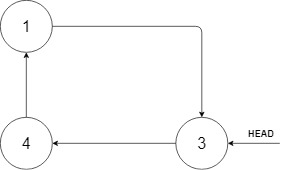
\includegraphics[width=150pt]{insert-into-a-cyclic-sorted-list-001.jpg}\\
\figcaption{before insert}\label{fig:insert-into-a-cyclic-sorted-list-001}
\end{center}

\begin{center}
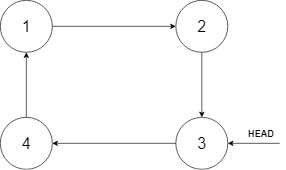
\includegraphics[width=150pt]{insert-into-a-cyclic-sorted-list-002.jpg}\\
\figcaption{before insert}\label{fig:insert-into-a-cyclic-sorted-list-002}
\end{center}

\subsubsection{分析}
Nil

\subsubsection{代碼}
\begin{Code}
// LeetCode
// 時間複雜度O(logn),空間複雜度O(n)
class Solution {
public:
    Node* insert(Node* head, int insertVal) {
        // edge case [1,1,1], target: 0
        // edge case [2,3,5,1], target: 0
        if (head == nullptr) {
            head = new Node(insertVal);
            head->next = head;
        }
        else {
            Node *cur = head->next;
            Node *prev = head;
            Node *pivot = nullptr;
            while (!(cur->val >= insertVal && prev->val < insertVal)) {
                if (prev->val > cur->val)
                    pivot = prev; // 找出邊界, case [2,3,5,1], target: 0

                prev = cur;
                cur = cur->next;

                if (cur == head->next) break; // 走了一個循環也沒有結果
            }
            if (cur == head->next && pivot)
                pivot->next = new Node(insertVal, pivot->next);
            else
                prev->next = new Node(insertVal, cur);
        }
        return head;
    }
};
\end{Code}


\subsubsection{相關題目}
\begindot
\item 無
\myenddot


\subsection{LRU Cache}
\label{sec:lru-cache}


\subsubsection{描述}
Design and implement a data structure for Least Recently Used (LRU) cache. It should support the following operations: get and set.

\fn{get(key)} - Get the value (will always be positive) of the key if the key exists in the cache, otherwise return -1.

\fn{set(key, value)} - Set or insert the value if the key is not already present. When the cache reached its capacity, it should invalidate the least recently used item before inserting a new item.


\subsubsection{分析}
為了使查找、插入和刪除都有較高的性能,我們使用一個雙向鏈表(\fn{std::list})和一個哈希表(\fn{std::unordered_map}),因為:
\begin{itemize}
\item{哈希表保存每個節點的地址,可以基本保證在$O(1)$時間內查找節點}
\item{雙向鏈表插入和刪除效率高,單向鏈表插入和刪除時,還要查找節點的前驅節點}
\end{itemize}

具體實現細節:
\begin{itemize}
\item{越靠近鏈表頭部,表示節點上次訪問距離現在時間最短,尾部的節點表示最近訪問最少}
\item{訪問節點時,如果節點存在,把該節點交換到鏈表頭部,同時更新hash表中該節點的地址}
\item{插入節點時,如果cache的size達到了上限capacity,則刪除尾部節點,同時要在hash表中刪除對應的項;新節點插入鏈表頭部}
\end{itemize}


\subsubsection{代碼}
\begin{Code}
// LeetCode, LRU Cache
// 時間複雜度O(logn),空間複雜度O(n)
class LRUCache{
private:
    struct CacheNode {
        int key;
        int value;
        CacheNode(int k, int v) :key(k), value(v){}
    };
public:
    LRUCache(int capacity) {
        this->capacity = capacity;
    }

    int get(int key) {
        if (cacheMap.find(key) == cacheMap.end()) return -1;

        // 把當前訪問的節點移到鏈表頭部,並且更新map中該節點的地址
        cacheList.splice(cacheList.begin(), cacheList, cacheMap[key]);
        cacheMap[key] = cacheList.begin();
        return cacheMap[key]->value;
    }

    void set(int key, int value) {
        if (this->capacity == 0) return;
        if (cacheMap.find(key) == cacheMap.end()) {
            if (cacheList.size() == capacity) { //刪除鏈表尾部節點(最少訪問的節點)
                cacheMap.erase(cacheList.back().key);
                cacheList.pop_back();
            }
            // 插入新節點到鏈表頭部, 並且在map中增加該節點
            cacheList.push_front(CacheNode(key, value));
            cacheMap[key] = cacheList.begin();
        } else {
            //更新節點的值,把當前訪問的節點移到鏈表頭部,並且更新map中該節點的地址
            cacheMap[key]->value = value;
            cacheList.splice(cacheList.begin(), cacheList, cacheMap[key]);
            cacheMap[key] = cacheList.begin();
        }
    }
private:
    list<CacheNode> cacheList;
    unordered_map<int, list<CacheNode>::iterator> cacheMap;
    int capacity;
};
\end{Code}


\subsubsection{相關題目}
\begindot
\item 無
\myenddot

\section{雙鏈表} %%%%%%%%%%%%%%%%%%%%%%%%%%%%%%

雙鏈表節點的定義如下:
\begin{Code}
// 雙鏈表節點
class Node {
public:
    int val;
    Node* prev;
    Node* next;
    Node* child;
};
\end{Code}

\subsection{Flatten a Multilevel Doubly Linked List}
\label{sec:flatten-a-multilevel-doubly-linked-list}


\subsubsection{描述}
You are given a doubly linked list which in addition to the next and previous pointers, it could have a child pointer, which may or may not point to a separate doubly linked list. These child lists may have one or more children of their own, and so on, to produce a multilevel data structure, as shown in the example below.

Flatten the list so that all the nodes appear in a single-level, doubly linked list. You are given the head of the first level of the list.

\begin{center}
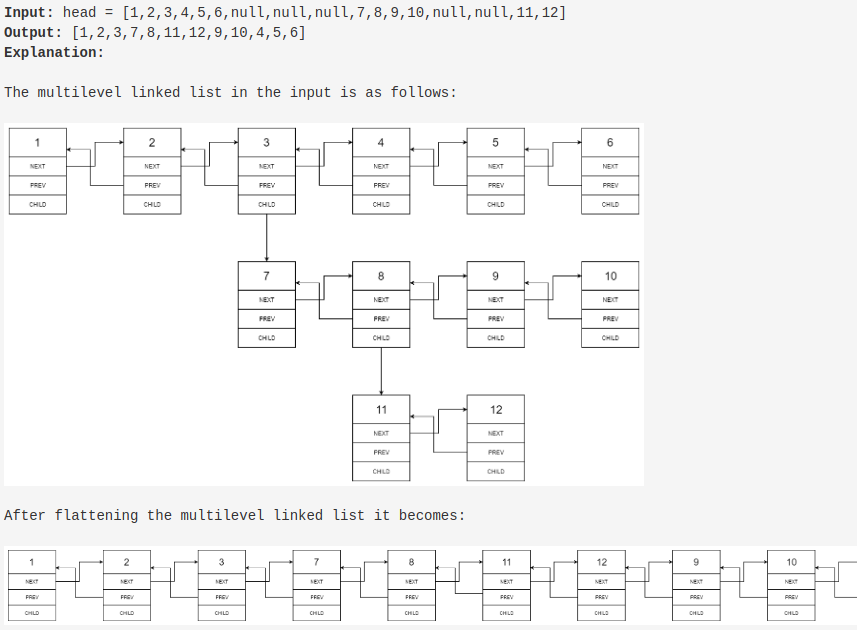
\includegraphics[width=300pt]{flatten-a-multilevel-doubly-list.png}\\
\figcaption{candy crush}\label{fig:flatten-a-multilevel-double-list}
\end{center}

\subsubsection{分析}
Nil

\subsubsection{遞歸版}
\begin{Code}
// LeetCode
// 時間複雜度O(n),空間複雜度O(1)
class Solution {
public:
    Node* flatten(Node* head) {
        for (Node *cur = head; cur; ) {
            if (cur->child == nullptr)
                cur = cur->next;
            else {
                cur->next = flatten_(cur->child, cur->next);
                cur->next->prev = cur;
                cur->child = nullptr;
            }
        }
        return head;
    }
private:
    Node *flatten_(Node* head, Node *tail) {
        Node *cur = head;
        while (cur->next) {
            if (cur->child == nullptr)
                cur = cur->next;
            else {
                Node *next = cur->next;
                cur->next = flatten_(cur->child, next);
                cur->next->prev = cur;
                cur->child = nullptr;
                cur = next;
            }
        }
        cur->next = tail;
        if (tail)
            tail->prev = cur;

        return head;
    }
};
\end{Code}

\subsubsection{Stack}
\begin{Code}
// LeetCode
// 時間複雜度O(n),空間複雜度O(1)
class Solution {
public:
    Node* flatten(Node* head) {
        if (head == nullptr) return head;

        stack<Node*> cache;

        Node *prev = nullptr;
        cache.push(head);
        while (!cache.empty()) {
            Node *cur = cache.top();
            cache.pop();

            if (prev)
                prev->next = cur;
            cur->prev = prev;

            if (cur->next) cache.push(cur->next);
            if (cur->child) cache.push(cur->child);
            cur->child = nullptr;

            prev = cur;
        }

        return head;
    }
};
\end{Code}

\subsubsection{相關題目}

\begindot
\item Nil
\myenddot

\chapter{字符串}


\section{Valid Palindrome} %%%%%%%%%%%%%%%%%%%%%%%%%%%%%%
\label{sec:valid-palindrome}


\subsubsection{描述}
Given a string, determine if it is a palindrome, considering only alphanumeric characters and ignoring cases.

For example,\\
\code{"A man, a plan, a canal: Panama"} is a palindrome.\\
\code{"race a car"} is not a palindrome.

Note:
Have you consider that the string might be empty? This is a good question to ask during an interview.

For the purpose of this problem, we define empty string as valid palindrome.


\subsubsection{分析}
無


\subsubsection{代碼}
\begin{Code}
// Leet Code, Valid Palindrome
// 時間複雜度O(n),空間複雜度O(1)
class Solution {
public:
    bool isPalindrome(string s) {
        transform(s.begin(), s.end(), s.begin(), ::tolower);
        auto left = s.begin(), right = prev(s.end());
        while (left < right) {
            if (!::isalnum(*left))  ++left;
            else if (!::isalnum(*right)) --right;
            else if (*left != *right) return false;
            else { left++, right--; }
        }
        return true;
    }
};
\end{Code}


\subsubsection{相關題目}
\begindot
\item Palindrome Number, 見 \S \ref{sec:palindrome-number}
\myenddot


\section{Implement strStr()} %%%%%%%%%%%%%%%%%%%%%%%%%%%%%%
\label{sec:strstr}


\subsubsection{描述}
Implement strStr().

Returns a pointer to the first occurrence of needle in haystack, or null if needle is not part of haystack.


\subsubsection{分析}
暴力算法的複雜度是 $O(m*n)$,代碼如下。更高效的的算法有KMP算法、Boyer-Mooer算法和Rabin-Karp算法。面試中暴力算法足夠了,一定要寫得沒有BUG。


\subsubsection{暴力匹配}
\begin{Code}
// LeetCode, Implement strStr()
// 暴力解法,時間複雜度O(N*M),空間複雜度O(1)
class Solution {
public:
    int strStr(const string& haystack, const string& needle) {
        if (needle.empty()) return 0;

        const int N = haystack.size() - needle.size() + 1;
        for (int i = 0; i < N; i++) {
            int j = i;
            int k = 0;
            while (j < haystack.size() && k < needle.size() && haystack[j] == needle[k]) {
                j++;
                k++;
            }
            if (k == needle.size()) return i;
        }
        return -1;
    }
};
\end{Code}


\subsubsection{KMP}
\begin{Code}
// LeetCode, Implement strStr()
// KMP,時間複雜度O(N+M),空間複雜度O(M)
class Solution {
public:
    int strStr(const string& haystack, const string& needle) {
        return kmp(haystack.c_str(), needle.c_str());
    }
private:
    /*
     * @brief 計算部分匹配表,即next數組.
     *
     * @param[in] pattern 模式串
     * @param[out] next next數組
     * @return 無
     */
    static void compute_prefix(const char *pattern, int next[]) {
        int i;
        int j = -1;
        const int m = strlen(pattern);

        next[0] = j;
        for (i = 1; i < m; i++) {
            while (j > -1 && pattern[j + 1] != pattern[i]) j = next[j];

            if (pattern[i] == pattern[j + 1]) j++;
            next[i] = j;
        }
    }

    /*
     * @brief KMP算法.
     *
     * @param[in] text 文本
     * @param[in] pattern 模式串
     * @return 成功則返回第一次匹配的位置,失敗則返回-1
     */
    static int kmp(const char *text, const char *pattern) {
        int i;
        int j = -1;
        const int n = strlen(text);
        const int m = strlen(pattern);
        if (n == 0 && m == 0) return 0; /* "","" */
        if (m == 0) return 0;  /* "a","" */
        int *next = (int*)malloc(sizeof(int) * m);

        compute_prefix(pattern, next);

        for (i = 0; i < n; i++) {
            while (j > -1 && pattern[j + 1] != text[i]) j = next[j];

            if (text[i] == pattern[j + 1]) j++;
            if (j == m - 1) {
                free(next);
                return i-j;
            }
        }

        free(next);
        return -1;
    }
};
\end{Code}


\subsubsection{相關題目}
\begindot
\item String to Integer (atoi) ,見 \S \ref{sec:string-to-integer}
\myenddot


\section{String to Integer (atoi)} %%%%%%%%%%%%%%%%%%%%%%%%%%%%%%
\label{sec:string-to-integer}


\subsubsection{描述}
Implement \fn{atoi} to convert a string to an integer.

\textbf{Hint}: Carefully consider all possible input cases. If you want a challenge, please do not see below and ask yourself what are the possible input cases.

\textbf{Notes}: It is intended for this problem to be specified vaguely (ie, no given input specs). You are responsible to gather all the input requirements up front.

\textbf{Requirements for atoi}:

The function first discards as many whitespace characters as necessary until the first non-whitespace character is found. Then, starting from this character, takes an optional initial plus or minus sign followed by as many numerical digits as possible, and interprets them as a numerical value.

The string can contain additional characters after those that form the integral number, which are ignored and have no effect on the behavior of this function.

If the first sequence of non-whitespace characters in str is not a valid integral number, or if no such sequence exists because either str is empty or it contains only whitespace characters, no conversion is performed.

If no valid conversion could be performed, a zero value is returned. If the correct value is out of the range of representable values, \code{INT_MAX (2147483647)} or \code{INT_MIN (-2147483648)} is returned.

\subsubsection{分析}
細節題。注意幾個測試用例:
\begin{enumerate}
\item 不規則輸入,但是有效,"-3924x8fc", "  +  413",
\item 無效格式," ++c", " ++1"
\item 溢出數據,"2147483648"
\end{enumerate}

\subsubsection{代碼}
\begin{Code}
// LeetCode, String to Integer (atoi)
// 時間複雜度O(n),空間複雜度O(1)
class Solution {
public:
    int myAtoi(const string &str) {
        int num = 0;
        int sign = 1;
        const int n = str.length();
        int i = 0;

        while (str[i] == ' ' && i < n) i++;

        if (str[i] == '+') {
            i++;
        } else if (str[i] == '-') {
            sign = -1;
            i++;
        }

        for (; i < n; i++) {
            if (str[i] < '0' || str[i] > '9')
                break;
            if (num > INT_MAX / 10 ||
                            (num == INT_MAX / 10 &&
                                    (str[i] - '0') > INT_MAX % 10)) {
                return sign == -1 ? INT_MIN : INT_MAX;
            }
            num = num * 10 + str[i] - '0';
        }
        return num * sign;
    }
};
\end{Code}


\subsubsection{相關題目}
\begindot
\item Implement strStr() ,見 \S \ref{sec:strstr}
\myenddot


\section{Add Binary} %%%%%%%%%%%%%%%%%%%%%%%%%%%%%%
\label{sec:add-binary}


\subsubsection{描述}
Given two binary strings, return their sum (also a binary string).

For example,
\begin{Code}
a = "11"
b = "1"
\end{Code}
Return {\small \fontspec{Latin Modern Mono} "100"}.


\subsubsection{分析}
無


\subsubsection{代碼}
\begin{Code}
//LeetCode, Add Binary
// 時間複雜度O(n),空間複雜度O(1)
class Solution {
public:
    string addBinary(string a, string b) {
        string result;
        const size_t n = a.size() > b.size() ? a.size() : b.size();
        reverse(a.begin(), a.end());
        reverse(b.begin(), b.end());
        int carry = 0;
        for (size_t i = 0; i < n; i++) {
            const int ai = i < a.size() ? a[i] - '0' : 0;
            const int bi = i < b.size() ? b[i] - '0' : 0;
            const int val = (ai + bi + carry) % 2;
            carry = (ai + bi + carry) / 2;
            result.insert(result.begin(), val + '0');
        }
        if (carry == 1) {
            result.insert(result.begin(), '1');
        }
        return result;
    }
};
\end{Code}


\subsubsection{相關題目}
\begindot
\item Add Two Numbers, 見 \S \ref{sec:add-two-numbers}
\myenddot


\section{Longest Palindromic Substring} %%%%%%%%%%%%%%%%%%%%%%%%%%%%%%
\label{sec:longest-palindromic-substring}


\subsubsection{描述}
Given a string $S$, find the longest palindromic substring in $S$. You may assume that the maximum length of $S$ is 1000, and there exists one unique longest palindromic substring.


\subsubsection{分析}
最長迴文子串,非常經典的題。

思路一:暴力枚舉,以每個元素為中間元素,同時從左右出發,複雜度$O(n^2)$。

思路二:記憶化搜索,複雜度$O(n^2)$。設\fn{f[i][j]} 表示[i,j]之間的最長迴文子串,遞推方程如下:
\begin{Code}
f[i][j] = if (i == j) S[i]
          if (S[i] == S[j] && f[i+1][j-1] == S[i+1][j-1]) S[i][j]
          else max(f[i+1][j-1], f[i][j-1], f[i+1][j])
\end{Code}

思路三:動規,複雜度$O(n^2)$。設狀態為\fn{f(i,j)},表示區間[i,j]是否為迴文串,則狀態轉移方程為
$$
f(i,j)=\begin{cases}
true & ,i=j\\
S[i]=S[j] & , j = i + 1 \\
S[i]=S[j] \text{ and } f(i+1, j-1) & , j > i + 1
\end{cases}
$$

思路四:Manacher’s Algorithm, 複雜度$O(n)$。詳細解釋見 \myurl{http://leetcode.com/2011/11/longest-palindromic-substring-part-ii.html} 。


\subsubsection{備忘錄法}
\begin{Code}
// LeetCode, Longest Palindromic Substring
// 備忘錄法,會超時
// 時間複雜度O(n^2),空間複雜度O(n^2)
typedef string::const_iterator Iterator;

namespace std {
template<>
struct hash<pair<Iterator, Iterator>> {
    size_t operator()(pair<Iterator, Iterator> const& p) const {
        return ((size_t) &(*p.first)) ^ ((size_t) &(*p.second));
    }
};
}

class Solution {
public:
    string longestPalindrome(string const& s) {
        cache.clear();
        return cachedLongestPalindrome(s.begin(), s.end());
    }

private:
    unordered_map<pair<Iterator, Iterator>, string> cache;

    string longestPalindrome(Iterator first, Iterator last) {
        size_t length = distance(first, last);

        if (length < 2) return string(first, last);

        auto s = cachedLongestPalindrome(next(first), prev(last));

        if (s.length() == length - 2 && *first == *prev(last))
            return string(first, last);

        auto s1 = cachedLongestPalindrome(next(first), last);
        auto s2 = cachedLongestPalindrome(first, prev(last));

        // return max(s, s1, s2)
        if (s.size() > s1.size()) return s.size() > s2.size() ? s : s2;
        else return s1.size() > s2.size() ? s1 : s2;
    }

    string cachedLongestPalindrome(Iterator first, Iterator last) {
        auto key = make_pair(first, last);
        auto pos = cache.find(key);

        if (pos != cache.end()) return pos->second;
        else return cache[key] = longestPalindrome(first, last);
    }
};
\end{Code}


\subsubsection{動規}
\begin{Code}
// LeetCode, Longest Palindromic Substring
// 動規,時間複雜度O(n^2),空間複雜度O(n^2)
class Solution {
public:
    string longestPalindrome(const string& s) {
        const int n = s.size();
        bool f[n][n];
        fill_n(&f[0][0], n * n, false);
        // 用 vector 會超時
        //vector<vector<bool> > f(n, vector<bool>(n, false));
        size_t max_len = 1, start = 0;  // 最長迴文子串的長度,起點

        for (size_t i = 0; i < s.size(); i++) {
            f[i][i] = true;
            for (size_t j = 0; j < i; j++) {  // [j, i]
                f[j][i] = (s[j] == s[i] && (i - j < 2 || f[j + 1][i - 1]));
                if (f[j][i] && max_len < (i - j + 1)) {
                    max_len = i - j + 1;
                    start = j;
                }
            }
        }
        return s.substr(start, max_len);
    }
};
\end{Code}


\subsubsection{Manacher’s Algorithm}
\begin{Code}
// LeetCode, Longest Palindromic Substring
// Manacher’s Algorithm
// 時間複雜度O(n),空間複雜度O(n)
class Solution {
public:
    // Transform S into T.
    // For example, S = "abba", T = "^#a#b#b#a#$".
    // ^ and $ signs are sentinels appended to each end to avoid bounds checking
    string preProcess(const string& s) {
        int n = s.length();
        if (n == 0) return "^$";

        string ret = "^";
        for (int i = 0; i < n; i++) ret += "#" + s.substr(i, 1);

        ret += "#$";
        return ret;
    }

    string longestPalindrome(string s) {
        string T = preProcess(s);
        const int n = T.length();
        // 以T[i]為中心,向左/右擴張的長度,不包含T[i]自己,
        // 因此 P[i]是源字符串中迴文串的長度
        int P[n];
        int C = 0, R = 0;

        for (int i = 1; i < n - 1; i++) {
            int i_mirror = 2 * C - i; // equals to i' = C - (i-C)

            P[i] = (R > i) ? min(R - i, P[i_mirror]) : 0;

            // Attempt to expand palindrome centered at i
            while (T[i + 1 + P[i]] == T[i - 1 - P[i]])
                P[i]++;

            // If palindrome centered at i expand past R,
            // adjust center based on expanded palindrome.
            if (i + P[i] > R) {
                C = i;
                R = i + P[i];
            }
        }

        // Find the maximum element in P.
        int max_len = 0;
        int center_index = 0;
        for (int i = 1; i < n - 1; i++) {
            if (P[i] > max_len) {
                max_len = P[i];
                center_index = i;
            }
        }

        return s.substr((center_index - 1 - max_len) / 2, max_len);
    }
};
\end{Code}


\subsubsection{相關題目}
\begindot
\item 無
\myenddot


\section{Regular Expression Matching} %%%%%%%%%%%%%%%%%%%%%%%%%%%%%%
\label{sec:regular-expression-matching}


\subsubsection{描述}
Implement regular expression matching with support for \fn{'.'} and \fn{'*'}.

\fn{'.'} Matches any single character.
\fn{'*'} Matches zero or more of the preceding element.

The matching should cover the entire input string (not partial).

The function prototype should be:
\begin{Code}
bool isMatch(const char *s, const char *p)
\end{Code}

Some examples:
\begin{Code}
isMatch("aa","a") → false
isMatch("aa","aa") → true
isMatch("aaa","aa") → false
isMatch("aa", "a*") → true
isMatch("aa", ".*") → true
isMatch("ab", ".*") → true
isMatch("aab", "c*a*b") → true
\end{Code}


\subsubsection{分析}
這是一道很有挑戰的題。


\subsubsection{遞歸版}
\begin{Code}
// LeetCode, Regular Expression Matching
// 遞歸版,時間複雜度O(n),空間複雜度O(1)
class Solution {
public:
    bool isMatch(const string& s, const string& p) {
        return isMatch(s.c_str(), p.c_str());
    }
private:
    bool isMatch(const char *s, const char *p) {
        if (*p == '\0') return *s == '\0';

        // next char is not '*', then must match current character
        if (*(p + 1) != '*') {
            if (*p == *s || (*p == '.' && *s != '\0'))
                return isMatch(s + 1, p + 1);
            else
                return false;
        } else { // next char is '*'
            while (*p == *s || (*p == '.' && *s != '\0')) {
                if (isMatch(s, p + 2))
                    return true;
                s++;
            }
            return isMatch(s, p + 2);
        }
    }
};
\end{Code}


\subsubsection{迭代版}
\begin{Code}

\end{Code}


\subsubsection{相關題目}
\begindot
\item Wildcard Matching, 見 \S \ref{sec:wildcard-matching}
\myenddot


\section{Wildcard Matching} %%%%%%%%%%%%%%%%%%%%%%%%%%%%%%
\label{sec:wildcard-matching}


\subsubsection{描述}
Implement wildcard pattern matching with support for \fn{'?'} and \fn{'*'}.

\fn{'?'} Matches any single character.
\fn{'*'} Matches any sequence of characters (including the empty sequence).

The matching should cover the entire input string (not partial).

The function prototype should be:
\begin{Code}
bool isMatch(const char *s, const char *p)
\end{Code}

Some examples:
\begin{Code}
isMatch("aa","a") → false
isMatch("aa","aa") → true
isMatch("aaa","aa") → false
isMatch("aa", "*") → true
isMatch("aa", "a*") → true
isMatch("ab", "?*") → true
isMatch("aab", "c*a*b") → false
\end{Code}


\subsubsection{分析}
跟上一題很類似。

主要是\fn{'*'}的匹配問題。\fn{p}每遇到一個\fn{'*'},就保留住當前\fn{'*'}的座標和\fn{s}的座標,然後\fn{s}從前往後掃描,如果不成功,則\fn{s++},重新掃描。


\subsubsection{遞歸版}
\begin{Code}
// LeetCode, Wildcard Matching
// 遞歸版,會超時,用於幫助理解題意
// 時間複雜度O(n!*m!),空間複雜度O(n)
class Solution {
public:
    bool isMatch(const string& s, const string& p) {
        return isMatch(s.c_str(), p.c_str());
    }
private:
    bool isMatch(const char *s, const char *p) {
        if (*p == '*') {
            while (*p == '*') ++p;  //skip continuous '*'
            if (*p == '\0') return true;
            while (*s != '\0' && !isMatch(s, p)) ++s;

            return *s != '\0';
        }
        else if (*p == '\0' || *s == '\0') return *p == *s;
        else if (*p == *s || *p == '?') return isMatch(++s, ++p);
        else return false;
    }
};
\end{Code}


\subsubsection{迭代版}
\begin{Code}
// LeetCode, Wildcard Matching
// 迭代版,時間複雜度O(n*m),空間複雜度O(1)
class Solution {
public:
    bool isMatch(const string& s, const string& p) {
        return isMatch(s.c_str(), p.c_str());
    }
private:
    bool isMatch(const char *s, const char *p) {
        bool star = false;
        const char *str, *ptr;
        for (str = s, ptr = p; *str != '\0'; str++, ptr++) {
            switch (*ptr) {
            case '?':
                break;
            case '*':
                star = true;
                s = str, p = ptr;
                while (*p == '*') p++;  //skip continuous '*'
                if (*p == '\0') return true;
                str = s - 1;
                ptr = p - 1;
                break;
            default:
                if (*str != *ptr) {
                    // 如果前面沒有'*',則匹配不成功
                    if (!star) return false;
                    s++;
                    str = s - 1;
                    ptr = p - 1;
                }
            }
        }
        while (*ptr == '*') ptr++;
        return (*ptr == '\0');
    }
};
\end{Code}


\subsubsection{相關題目}
\begindot
\item Regular Expression Matching, 見 \S \ref{sec:regular-expression-matching}
\myenddot


\section{Longest Common Prefix} %%%%%%%%%%%%%%%%%%%%%%%%%%%%%%
\label{sec:longest-common-prefix}


\subsubsection{描述}
Write a function to find the longest common prefix string amongst an array of strings.


\subsubsection{分析}
從位置0開始,對每一個位置比較所有字符串,直到遇到一個不匹配。


\subsubsection{縱向掃描}
\begin{Code}
// LeetCode, Longest Common Prefix
// 縱向掃描,從位置0開始,對每一個位置比較所有字符串,直到遇到一個不匹配
// 時間複雜度O(n1+n2+...)
// @author 周倩 (http://weibo.com/zhouditty)
class Solution {
public:
    string longestCommonPrefix(vector<string> &strs) {
        if (strs.empty()) return "";

        for (int idx = 0; idx < strs[0].size(); ++idx) { // 縱向掃描
            for (int i = 1; i < strs.size(); ++i) {
                if (strs[i][idx] != strs[0][idx]) return strs[0].substr(0,idx);
            }
        }
        return strs[0];
    }
};
\end{Code}


\subsubsection{橫向掃描}
\begin{Code}
// LeetCode, Longest Common Prefix
// 橫向掃描,每個字符串與第0個字符串,從左到右比較,直到遇到一個不匹配,
// 然後繼續下一個字符串
// 時間複雜度O(n1+n2+...)
class Solution {
public:
    string longestCommonPrefix(vector<string> &strs) {
        if (strs.empty()) return "";

        int right_most = strs[0].size() - 1;
        for (size_t i = 1; i < strs.size(); i++)
            for (int j = 0; j <= right_most; j++)
                if (strs[i][j] != strs[0][j])  // 不會越界,請參考string::[]的文檔
                    right_most = j - 1;

        return strs[0].substr(0, right_most + 1);
    }
};
\end{Code}


\subsubsection{相關題目}
\begindot
\item 無
\myenddot


\section{Valid Number} %%%%%%%%%%%%%%%%%%%%%%%%%%%%%%
\label{sec:valid-number}


\subsubsection{描述}
Validate if a given string is numeric.

Some examples:
\begin{Code}
"0" => true
" 0.1 " => true
"abc" => false
"1 a" => false
"2e10" => true
\end{Code}

Note: It is intended for the problem statement to be ambiguous. You should gather all requirements up front before implementing one.


\subsubsection{分析}
細節實現題。

本題的功能與標準庫中的\fn{strtod()}功能類似。


\subsubsection{有限自動機}
\begin{Code}
// LeetCode, Valid Number
// @author 龔陸安 (http://weibo.com/luangong)
// finite automata,時間複雜度O(n),空間複雜度O(n)
class Solution {
public:
    bool isNumber(const string& s) {
        enum InputType {
            INVALID,    // 0
            SPACE,      // 1
            SIGN,       // 2
            DIGIT,      // 3
            DOT,        // 4
            EXPONENT,   // 5
            NUM_INPUTS  // 6
        };
        const int transitionTable[][NUM_INPUTS] = {
                -1, 0, 3, 1, 2, -1, // next states for state 0
                -1, 8, -1, 1, 4, 5,     // next states for state 1
                -1, -1, -1, 4, -1, -1,     // next states for state 2
                -1, -1, -1, 1, 2, -1,     // next states for state 3
                -1, 8, -1, 4, -1, 5,     // next states for state 4
                -1, -1, 6, 7, -1, -1,     // next states for state 5
                -1, -1, -1, 7, -1, -1,     // next states for state 6
                -1, 8, -1, 7, -1, -1,     // next states for state 7
                -1, 8, -1, -1, -1, -1,     // next states for state 8
                };

        int state = 0;
        for (auto ch : s) {
            InputType inputType = INVALID;
            if (isspace(ch))
                inputType = SPACE;
            else if (ch == '+' || ch == '-')
                inputType = SIGN;
            else if (isdigit(ch))
                inputType = DIGIT;
            else if (ch == '.')
                inputType = DOT;
            else if (ch == 'e' || ch == 'E')
                inputType = EXPONENT;

            // Get next state from current state and input symbol
            state = transitionTable[state][inputType];

            // Invalid input
            if (state == -1) return false;
        }
        // If the current state belongs to one of the accepting (final) states,
        // then the number is valid
        return state == 1 || state == 4 || state == 7 || state == 8;

    }
};
\end{Code}


\subsubsection{使用strtod()}
\begin{Code}
// LeetCode, Valid Number
// @author 連城 (http://weibo.com/lianchengzju)
// 偷懶,直接用 strtod(),時間複雜度O(n)
class Solution {
public:
    bool isNumber (const string& s) {
        return isNumber(s.c_str());
    }
private:
    bool isNumber (char const* s) {
        char* endptr;
        strtod (s, &endptr);

        if (endptr == s) return false;

        for (; *endptr; ++endptr)
            if (!isspace (*endptr)) return false;

        return true;
    }
};
\end{Code}


\subsubsection{相關題目}
\begindot
\item 無
\myenddot


\section{Integer to Roman} %%%%%%%%%%%%%%%%%%%%%%%%%%%%%%
\label{sec:integer-to-roman}


\subsubsection{描述}
Given an integer, convert it to a roman numeral.

Input is guaranteed to be within the range from 1 to 3999.


\subsubsection{分析}
無


\subsubsection{代碼}
\begin{Code}
// LeetCode, Integer to Roman
// 時間複雜度O(num),空間複雜度O(1)
class Solution {
public:
    string intToRoman(int num) {
        const int radix[] = {1000, 900, 500, 400, 100, 90,
                50, 40, 10, 9, 5, 4, 1};
        const string symbol[] = {"M", "CM", "D", "CD", "C", "XC",
                "L", "XL", "X", "IX", "V", "IV", "I"};

        string roman;
        for (size_t i = 0; num > 0; ++i) {
            int count = num / radix[i];
            num %= radix[i];
            for (; count > 0; --count) roman += symbol[i];
        }
        return roman;
    }
};
\end{Code}


\subsubsection{相關題目}
\begindot
\item Roman to Integer, 見 \S \ref{sec:roman-to-integer}
\myenddot


\section{Roman to Integer} %%%%%%%%%%%%%%%%%%%%%%%%%%%%%%
\label{sec:roman-to-integer}


\subsubsection{描述}
Given a roman numeral, convert it to an integer.

Input is guaranteed to be within the range from 1 to 3999.


\subsubsection{分析}
從前往後掃描,用一個臨時變量記錄分段數字。

如果當前比前一個大,説明這一段的值應該是當前這個值減去上一個值。比如\fn{IV = 5 – 1};否則,將當前值加入到結果中,然後開始下一段記錄。比如\fn{VI = 5 + 1, II=1+1}


\subsubsection{代碼}
\begin{Code}
// LeetCode, Roman to Integer
// 時間複雜度O(n),空間複雜度O(1)
class Solution {
public:
    inline int map(const char c) {
        switch (c) {
        case 'I': return 1;
        case 'V': return 5;
        case 'X': return 10;
        case 'L': return 50;
        case 'C': return 100;
        case 'D': return 500;
        case 'M': return 1000;
        default: return 0;
        }
    }

    int romanToInt(const string& s) {
        int result = 0;
        for (size_t i = 0; i < s.size(); i++) {
            if (i > 0 && map(s[i]) > map(s[i - 1])) {
                result += (map(s[i]) - 2 * map(s[i - 1]));
            } else {
                result += map(s[i]);
            }
        }
        return result;
    }
};
\end{Code}


\subsubsection{相關題目}
\begindot
\item Integer to Roman, 見 \S \ref{sec:integer-to-roman}
\myenddot


\section{Count and Say} %%%%%%%%%%%%%%%%%%%%%%%%%%%%%%
\label{sec:count-and-say}


\subsubsection{描述}
The count-and-say sequence is the sequence of integers beginning as follows:
\begin{Code}
1, 11, 21, 1211, 111221, ...
\end{Code}

\fn{1} is read off as \fn{"one 1"} or \fn{11}.

\fn{11} is read off as \fn{"two 1s"} or \fn{21}.

\fn{21} is read off as \fn{"one 2"}, then \fn{"one 1"} or \fn{1211}.

Given an integer $n$, generate the nth sequence.

Note: The sequence of integers will be represented as a string.


\subsubsection{分析}
模擬。


\subsubsection{代碼}
\begin{Code}
// LeetCode, Count and Say
// @author 連城 (http://weibo.com/lianchengzju)
// 時間複雜度O(n^2),空間複雜度O(n)
class Solution {
public:
    string countAndSay(int n) {
        string s("1");

        while (--n)
            s = getNext(s);

        return s;
    }

    string getNext(const string &s) {
        stringstream ss;

        for (auto i = s.begin(); i != s.end(); ) {
            auto j = find_if(i, s.end(), bind1st(not_equal_to<char>(), *i));
            ss << distance(i, j) << *i;
            i = j;
        }

        return ss.str();
    }
};
\end{Code}


\subsubsection{相關題目}
\begindot
\item 無
\myenddot


\section{Anagrams} %%%%%%%%%%%%%%%%%%%%%%%%%%%%%%
\label{sec:anagrams}


\subsubsection{描述}
Given an array of strings, return all groups of strings that are anagrams.

Note: All inputs will be in lower-case.


\subsubsection{分析}
Anagram(迴文構詞法)是指打亂字母順序從而得到新的單詞,比如 \fn{"dormitory"} 打亂字母順序會變成 \fn{"dirty room"} ,\fn{"tea"} 會變成\fn{"eat"}。

迴文構詞法有一個特點:單詞裏的字母的種類和數目沒有改變,只是改變了字母的排列順序。因此,將幾個單詞按照字母順序排序後,若它們相等,則它們屬於同一組 anagrams 。


\subsubsection{代碼}
\begin{Code}
// LeetCode, Anagrams
// 時間複雜度O(n),空間複雜度O(n)
class Solution {
public:
    vector<string> anagrams(vector<string> &strs) {
        unordered_map<string, vector<string> > group;
        for (const auto &s : strs) {
            string key = s;
            sort(key.begin(), key.end());
            group[key].push_back(s);
        }

        vector<string> result;
        for (auto it = group.cbegin(); it != group.cend(); it++) {
            if (it->second.size() > 1)
                result.insert(result.end(), it->second.begin(), it->second.end());
        }
        return result;
    }
};
\end{Code}


\subsubsection{相關題目}
\begindot
\item 無
\myenddot


\section{Simplify Path} %%%%%%%%%%%%%%%%%%%%%%%%%%%%%%
\label{sec:simplify-path}


\subsubsection{描述}
Given an absolute path for a file (Unix-style), simplify it.

For example, \\
path = \fn{"/home/"}, => \fn{"/home"} \\
path = \fn{"/a/./b/../../c/"}, => \fn{"/c"} \\

Corner Cases:
\begindot
\item Did you consider the case where path = \fn{"/../"}? 
In this case, you should return \fn{"/"}.
\item 
Another corner case is the path might contain multiple slashes \fn{'/'} together, such as \fn{"/home//foo/"}.
In this case, you should ignore redundant slashes and return \fn{"/home/foo"}.
\myenddot


\subsubsection{分析}
很有實際價值的題目。


\subsubsection{代碼}
\begin{Code}
// LeetCode, Simplify Path
// 時間複雜度O(n),空間複雜度O(n)
class Solution {
public:
    string simplifyPath(const string& path) {
        vector<string> dirs; // 當做棧

        for (auto i = path.begin(); i != path.end();) {
            ++i;

            auto j = find(i, path.end(), '/');
            auto dir = string(i, j);

            if (!dir.empty() && dir != ".") {// 當有連續 '///'時,dir 為空
                if (dir == "..") {
                    if (!dirs.empty())
                        dirs.pop_back();
                } else
                    dirs.push_back(dir);
            }

            i = j;
        }

        stringstream out;
        if (dirs.empty()) {
            out << "/";
        } else {
            for (auto dir : dirs)
                out << '/' << dir;
        }

        return out.str();
    }
};
\end{Code}


\subsubsection{相關題目}
\begindot
\item 無
\myenddot


\section{Length of Last Word} %%%%%%%%%%%%%%%%%%%%%%%%%%%%%%
\label{sec:length-of-last-word}


\subsubsection{描述}
Given a string s consists of upper/lower-case alphabets and empty space characters \fn{' '}, return the length of last word in the string.

If the last word does not exist, return 0.

Note: A word is defined as a character sequence consists of non-space characters only.

For example, 
Given \fn{s = "Hello World"},
return 5.


\subsubsection{分析}
細節實現題。


\subsubsection{用 STL}
\begin{Code}
// LeetCode, Length of Last Word
// 偷懶,用 STL
// 時間複雜度O(n),空間複雜度O(1)
class Solution {
public:
    int lengthOfLastWord(const string& s) {
        auto first = find_if(s.rbegin(), s.rend(), ::isalpha);
        auto last = find_if_not(first, s.rend(), ::isalpha);
        return distance(first, last);
    }
};
\end{Code}


\subsubsection{順序掃描}
\begin{Code}
// LeetCode, Length of Last Word
// 順序掃描,記錄每個 word 的長度
// 時間複雜度O(n),空間複雜度O(1)
class Solution {
public:
    int lengthOfLastWord(const string& s) {
        return lengthOfLastWord(s.c_str());
    }
private:
    int lengthOfLastWord(const char *s) {
        int len = 0;
        while (*s) {
            if (*s++ != ' ')
                ++len;
            else if (*s && *s != ' ')
                len = 0;
        }
        return len;
    }
};
\end{Code}


\subsubsection{相關題目}
\begindot
\item 無
\myenddot

\chapter{棧和隊列}


\section{棧} %%%%%%%%%%%%%%%%%%%%%%%%%%%%%%


\subsection{Valid Parentheses} %%%%%%%%%%%%%%%%%%%%%%%%%%%%%%
\label{sec:valid-parentheses}


\subsubsection{描述}
Given a string containing just the characters \code{'(', ')', '\{', '\}', '['} and \code{']'}, determine if the input string is valid.

The brackets must close in the correct order, \code{"()"} and \code{"()[]{}"} are all valid but \code{"(]"} and \code{"([)]"} are not.


\subsubsection{分析}
無


\subsubsection{代碼}
\begin{Code}
// LeetCode, Valid Parentheses
// 時間複雜度O(n),空間複雜度O(n)
class Solution {
public:
    bool isValid (string const& s) {
        string left = "([{";
        string right = ")]}";
        stack<char> stk;

        for (auto c : s) {
            if (left.find(c) != string::npos) {
                stk.push (c);
            } else {
                if (stk.empty () || stk.top () != left[right.find (c)])
                    return false;
                else
                    stk.pop ();
            }
        }
        return stk.empty();
    }
};
\end{Code}


\subsubsection{相關題目}
\begindot
\item Generate Parentheses, 見 \S \ref{sec:generate-parentheses}
\item Longest Valid Parentheses, 見 \S \ref{sec:longest-valid-parentheses}
\myenddot


\subsection{Longest Valid Parentheses} %%%%%%%%%%%%%%%%%%%%%%%%%%%%%%
\label{sec:longest-valid-parentheses}


\subsubsection{描述}
Given a string containing just the characters \code{'('} and \code{')'}, find the length of the longest valid (well-formed) parentheses substring.

For \code{"(()"}, the longest valid parentheses substring is \code{"()"}, which has length = 2.

Another example is \code{")()())"}, where the longest valid parentheses substring is \code{"()()"}, which has length = 4.


\subsubsection{分析}
無


\subsubsection{使用棧}
\begin{Code}
// LeetCode, Longest Valid Parenthese
// 使用棧,時間複雜度O(n),空間複雜度O(n)
class Solution {
public:
    int longestValidParentheses(const string& s) {
        int max_len = 0, last = -1; // the position of the last ')'
        stack<int> lefts;  // keep track of the positions of non-matching '('s

        for (int i = 0; i < s.size(); ++i) {
            if (s[i] =='(') {
                lefts.push(i);
            } else {
                if (lefts.empty()) {
                    // no matching left
                    last = i;
                } else {
                    // find a matching pair
                    lefts.pop();
                    if (lefts.empty()) {
                        max_len = max(max_len, i-last);
                    } else {
                        max_len = max(max_len, i-lefts.top());
                    }
                }
            }
        }
        return max_len;
    }
};
\end{Code}

\subsubsection{Dynamic Programming, One Pass}
\begin{Code}
// LeetCode, Longest Valid Parenthese
// 時間複雜度O(n),空間複雜度O(n)
// @author 一隻傑森(http://weibo.com/wjson)
class Solution {
public:
    int longestValidParentheses(const string& s) {
        vector<int> f(s.size(), 0);
        int ret = 0;
        for (int i = s.size() - 2; i >= 0; --i) {
            int match = i + f[i + 1] + 1;
            // case: "((...))"
            if (s[i] == '(' && match < s.size() && s[match] == ')') {
                f[i] = f[i + 1] + 2;
                // if a valid sequence exist afterwards "((...))()"
                if (match + 1 < s.size()) f[i] += f[match + 1];
            }
            ret = max(ret, f[i]);
        }
        return ret;
    }
};
\end{Code}


\subsubsection{兩遍掃描}
\begin{Code}
// LeetCode, Longest Valid Parenthese
// 兩遍掃描,時間複雜度O(n),空間複雜度O(1)
// @author 曹鵬(http://weibo.com/cpcs)
class Solution {
public:
    int longestValidParentheses(const string& s) {
        int answer = 0, depth = 0, start = -1;
        for (int i = 0; i < s.size(); ++i) {
            if (s[i] == '(') {
                ++depth;
            } else {
                --depth;
                if (depth < 0) {
                    start = i;
                    depth = 0;
                } else if (depth == 0) {
                    answer = max(answer, i - start);
                }
            }
        }

        depth = 0;
        start = s.size();
        for (int i = s.size() - 1; i >= 0; --i) {
            if (s[i] == ')') {
                ++depth;
            } else {
                --depth;
                if (depth < 0) {
                    start = i;
                    depth = 0;
                } else if (depth == 0) {
                    answer = max(answer, start - i);
                }
            }
        }
        return answer;
    }
};
\end{Code}


\subsubsection{相關題目}
\begindot
\item Valid Parentheses, 見 \S \ref{sec:valid-parentheses}
\item Generate Parentheses, 見 \S \ref{sec:generate-parentheses}
\myenddot


\subsection{Largest Rectangle in Histogram} %%%%%%%%%%%%%%%%%%%%%%%%%%%%%%
\label{sec:largest-rectangle-in-histogram}


\subsubsection{描述}
Given $n$ non-negative integers representing the histogram's bar height where the width of each bar is 1, find the area of largest rectangle in the histogram.

\begin{center}
\includegraphics[width=120pt]{histogram.png}\\
\figcaption{Above is a histogram where width of each bar is 1, given height = \fn{[2,1,5,6,2,3]}.}\label{fig:histogram}
\end{center}

\begin{center}
\includegraphics[width=120pt]{histogram-area.png}\\
\figcaption{The largest rectangle is shown in the shaded area, which has area = 10 unit.}\label{fig:histogram-area}
\end{center}

For example,
Given height = \fn{[2,1,5,6,2,3]},
return 10.


\subsubsection{分析}
簡單的,類似於 Container With Most Water(\S \ref{sec:container-with-most-water}),對每個柱子,左右擴展,直到碰到比自己矮的,計算這個矩形的面積,用一個變量記錄最大的面積,複雜度$O(n^2)$,會超時。

如圖\S \ref{fig:histogram-area}所示,從左到右處理直方,當$i=4$時,小於當前棧頂(即直方3),對於直方3,無論後面還是前面的直方,都不可能得到比目前棧頂元素更高的高度了,處理掉直方3(計算從直方3到直方4之間的矩形的面積,然後從棧裏彈出);對於直方2也是如此;直到碰到比直方4更矮的直方1。

這就意味着,可以維護一個遞增的棧,每次比較棧頂與當前元素。如果當前元素大於棧頂元素,則入棧,否則合併現有棧,直至棧頂元素小於當前元素。結尾時入棧元素0,重複合併一次。


\subsubsection{代碼}
\begin{Code}
// LeetCode, Largest Rectangle in Histogram
// 時間複雜度O(n),空間複雜度O(n)
class Solution {
public:
    int largestRectangleArea(vector<int> &height) {
        stack<int> s;
        height.push_back(0);
        int result = 0;
        for (int i = 0; i < height.size(); ) {
            if (s.empty() || height[i] > height[s.top()])
                s.push(i++);
            else {
                int tmp = s.top();
                s.pop();
                result = max(result,
                        height[tmp] * (s.empty() ? i : i - s.top() - 1));
            }
        }
        return result;
    }
};
\end{Code}


\subsubsection{相關題目}
\begindot
\item Trapping Rain Water, 見 \S \ref{sec:trapping-rain-water}
\item Container With Most Water, 見 \S \ref{sec:container-with-most-water}
\myenddot


\subsection{Evaluate Reverse Polish Notation} %%%%%%%%%%%%%%%%%%%%%%%%%%%%%%
\label{sec:evaluate-reverse-polish-notation}


\subsubsection{描述}
Evaluate the value of an arithmetic expression in Reverse Polish Notation.

Valid operators are \fn{+, -, *, /}. Each operand may be an integer or another expression.

Some examples:
\begin{Code}
  ["2", "1", "+", "3", "*"] -> ((2 + 1) * 3) -> 9
  ["4", "13", "5", "/", "+"] -> (4 + (13 / 5)) -> 6
\end{Code}


\subsubsection{分析}
無


\subsubsection{遞歸版}
\begin{Code}
// LeetCode, Evaluate Reverse Polish Notation
// 遞歸,時間複雜度O(n),空間複雜度O(logn)
class Solution {
public:
    int evalRPN(vector<string> &tokens) {
        int x, y;
        auto token = tokens.back();  tokens.pop_back();
        if (is_operator(token))  {
            y = evalRPN(tokens);
            x = evalRPN(tokens);
            if (token[0] == '+')       x += y;
            else if (token[0] == '-')  x -= y;
            else if (token[0] == '*')  x *= y;
            else                       x /= y;
        } else  {
            size_t i;
            x = stoi(token, &i);
        }
        return x;
    }
private:
    bool is_operator(const string &op) {
        return op.size() == 1 && string("+-*/").find(op) != string::npos;
    }
};
\end{Code}


\subsubsection{迭代版}
\begin{Code}
// LeetCode, Max Points on a Line
// 迭代,時間複雜度O(n),空間複雜度O(logn)
class Solution {
public:
    int evalRPN(vector<string> &tokens) {
        stack<string> s;
        for (auto token : tokens) {
            if (!is_operator(token)) {
                s.push(token);
            } else {
                int y = stoi(s.top());
                s.pop();
                int x = stoi(s.top());
                s.pop();
                if (token[0] == '+')       x += y;
                else if (token[0] == '-')  x -= y;
                else if (token[0] == '*')  x *= y;
                else                       x /= y;
                s.push(to_string(x));
            }
        }
        return stoi(s.top());
    }
private:
    bool is_operator(const string &op) {
        return op.size() == 1 && string("+-*/").find(op) != string::npos;
    }
};
\end{Code}


\subsubsection{相關題目}
\begindot
\item 無
\myenddot


\section{隊列} %%%%%%%%%%%%%%%%%%%%%%%%%%%%%%

\subsection{Sliding Window Maximum} %%%%%%%%%%%%%%%%%%%%%%%%%%%%%%
\label{sec:sliding-window-maximum}


\subsubsection{描述}
Given an array nums, there is a sliding window of size k which is moving from the very left of the array to the very right. You can only see the k numbers in the window. Each time the sliding window moves right by one position. Return the max sliding window.


\textbf{Follow up:}
Could you solve it in linear time?

\textbf{Example:}
\begin{Code}
Input: nums = [1,3,-1,-3,5,3,6,7], and k = 3
Output: [3,3,5,5,6,7]
Explanation:

Window position                Max
---------------               -----
[1  3  -1] -3  5  3  6  7       3
 1 [3  -1  -3] 5  3  6  7       3
 1  3 [-1  -3  5] 3  6  7       5
 1  3  -1 [-3  5  3] 6  7       5
 1  3  -1  -3 [5  3  6] 7       6
 1  3  -1  -3  5 [3  6  7]      7
\end{Code}


\subsubsection{分析}
以 deque 來追踪視窗內的指標, 移除老去的指標, 移除數值太細的元素指標


\subsubsection{Code}
\begin{Code}
// LeetCode
// 迭代,時間複雜度O(n),空間複雜度O(n)
class Solution {
public:
    vector<int> maxSlidingWindow(vector<int>& nums, int k) {
        int N = nums.size();
        if (N < k) return vector<int>();

        vector<int> result; result.reserve(N-k+1);
        deque<int> indexList;

        // 預準首 K 項
        for (size_t i = 0; i < k; i++)
        {
            while (!indexList.empty() && nums[indexList.back()] < nums[i])
                indexList.pop_back();
            indexList.push_back(i);
        }
        result.push_back(nums[indexList.front()]);

        // 完成剩下的元素
        for (size_t i = k; i < nums.size(); i++)
        {
            // 移除老去的元素
            while (!indexList.empty() && indexList.front() < i-k+1)
                indexList.pop_front();

            // 移除數值太細的元素
            while (!indexList.empty() && nums[indexList.back()] < nums[i])
                indexList.pop_back();
            indexList.push_back(i);

            result.push_back(nums[indexList.front()]);
        }

        return result;
    }
};
\end{Code}


\subsubsection{相關題目}
\begindot
\item 無
\myenddot

\chapter{樹}

LeetCode 上二叉樹的節點定義如下:
\begin{Code}
// 樹的節點
struct TreeNode {
    int val;
    TreeNode *left;
    TreeNode *right;
    TreeNode(int x) : val(x), left(nullptr), right(nullptr) { }
};
\end{Code}


\section{二叉樹的遍歷} %%%%%%%%%%%%%%%%%%%%%%%%%%%%%%

樹的遍歷有兩類:深度優先遍歷和寬度優先遍歷。深度優先遍歷又可分為兩種:先根(次序)遍歷和後根(次序)遍歷。

樹的先根遍歷是:先訪問樹的根結點,然後依次先根遍歷根的各棵子樹。樹的先跟遍歷的結果與對應二叉樹(孩子兄弟表示法)的先序遍歷的結果相同。

樹的後根遍歷是:先依次後根遍歷樹根的各棵子樹,然後訪問根結點。樹的後跟遍歷的結果與對應二叉樹的中序遍歷的結果相同。

二叉樹的先根遍歷有:\textbf{先序遍歷}(root->left->right),root->right->left;後根遍歷有:\textbf{後序遍歷}(left->right->root),right->left->root;二叉樹還有個一般的樹沒有的遍歷次序,\textbf{中序遍歷}(left->root->right)。


\subsection{Binary Tree Preorder Traversal}
\label{sec:binary-tree-preorder-traversal}


\subsubsection{描述}
Given a binary tree, return the \emph{preorder} traversal of its nodes' values.

For example:
Given binary tree \code{\{1,\#,2,3\}},
\begin{Code}
 1
  \
   2
  /
 3
\end{Code}
return \code{\[1,2,3\]}.

Note: Recursive solution is trivial, could you do it iteratively?


\subsubsection{分析}
用棧或者Morris遍歷。


\subsubsection{棧}
\begin{Code}
// LeetCode, Binary Tree Preorder Traversal
// 使用棧,時間複雜度O(n),空間複雜度O(n)
class Solution {
public:
    vector<int> preorderTraversal(TreeNode *root) {
        vector<int> result;
        stack<const TreeNode *> s;
        if (root != nullptr) s.push(root);

        while (!s.empty()) {
            const TreeNode *p = s.top();
            s.pop();
            result.push_back(p->val);

            if (p->right != nullptr) s.push(p->right);
            if (p->left != nullptr) s.push(p->left);
        }
        return result;
    }
};
\end{Code}


\subsubsection{Morris先序遍歷}
\begin{Code}
// LeetCode, Binary Tree Preorder Traversal
// Morris先序遍歷,時間複雜度O(n),空間複雜度O(1)
class Solution {
public:
    vector<int> preorderTraversal(TreeNode *root) {
        vector<int> result;
        TreeNode *cur = root, *prev = nullptr;

        while (cur != nullptr) {
            if (cur->left == nullptr) {
                result.push_back(cur->val);
                prev = cur; /* cur剛剛被訪問過 */
                cur = cur->right;
            } else {
                /* 查找前驅 */
                TreeNode *node = cur->left;
                while (node->right != nullptr && node->right != cur)
                    node = node->right;

                if (node->right == nullptr) { /* 還沒線索化,則建立線索 */
                    result.push_back(cur->val); /* 僅這一行的位置與中序不同 */
                    node->right = cur;
                    prev = cur; /* cur剛剛被訪問過 */
                    cur = cur->left;
                } else {    /* 已經線索化,則刪除線索  */
                    node->right = nullptr;
                    /* prev = cur; 不能有這句,cur已經被訪問 */
                    cur = cur->right;
                }
            }
        }
        return result;
    }
};
\end{Code}


\subsubsection{相關題目}
\begindot
\item Binary Tree Inorder Traversal,見 \S \ref{sec:binary-tree-inorder-traversal}
\item Binary Tree Postorder Traversal,見 \S \ref{sec:binary-tree-postorder-traversal}
\item Recover Binary Search Tree,見 \S \ref{sec:recover-binary-search-tree}
\myenddot


\subsection{Binary Tree Inorder Traversal}
\label{sec:binary-tree-inorder-traversal}


\subsubsection{描述}
Given a binary tree, return the \emph{inorder} traversal of its nodes' values.

For example:
Given binary tree \code{\{1,\#,2,3\}},
\begin{Code}
 1
  \
   2
  /
 3
\end{Code}
return \code{\[1,3,2\]}.

Note: Recursive solution is trivial, could you do it iteratively?


\subsubsection{分析}
用棧或者Morris遍歷。


\subsubsection{棧}
\begin{Code}
// LeetCode, Binary Tree Inorder Traversal
// 使用棧,時間複雜度O(n),空間複雜度O(n)
class Solution {
public:
    vector<int> inorderTraversal(TreeNode *root) {
        vector<int> result;
        stack<const TreeNode *> s;
        const TreeNode *p = root;

        while (!s.empty() || p != nullptr) {
            if (p != nullptr) {
                s.push(p);
                p = p->left;
            } else {
                p = s.top();
                s.pop();
                result.push_back(p->val);
                p = p->right;
            }
        }
        return result;
    }
};
\end{Code}


\subsubsection{Morris中序遍歷}
\begin{Code}
// LeetCode, Binary Tree Inorder Traversal
// Morris中序遍歷,時間複雜度O(n),空間複雜度O(1)
class Solution {
public:
    vector<int> inorderTraversal(TreeNode *root) {
        vector<int> result;
        TreeNode *cur = root, *prev = nullptr;

        while (cur != nullptr) {
            if (cur->left == nullptr) {
                result.push_back(cur->val);
                prev = cur;
                cur = cur->right;
            } else {
                /* 查找前驅 */
                TreeNode *node = cur->left;
                while (node->right != nullptr && node->right != cur)
                    node = node->right;

                if (node->right == nullptr) { /* 還沒線索化,則建立線索 */
                    node->right = cur;
                    /* prev = cur; 不能有這句,cur還沒有被訪問 */
                    cur = cur->left;
                } else {    /* 已經線索化,則訪問節點,並刪除線索  */
                    result.push_back(cur->val);
                    node->right = nullptr;
                    prev = cur;
                    cur = cur->right;
                }
            }
        }
        return result;
    }
};
\end{Code}


\subsubsection{相關題目}
\begindot
\item Binary Tree Preorder Traversal,見 \S \ref{sec:binary-tree-preorder-traversal}
\item Binary Tree Postorder Traversal,見 \S \ref{sec:binary-tree-postorder-traversal}
\item Recover Binary Search Tree,見 \S \ref{sec:recover-binary-search-tree}
\myenddot


\subsection{Binary Tree Postorder Traversal}
\label{sec:binary-tree-postorder-traversal}


\subsubsection{描述}
Given a binary tree, return the \emph{postorder} traversal of its nodes' values.

For example:
Given binary tree \code{\{1,\#,2,3\}},
\begin{Code}
 1
  \
   2
  /
 3
\end{Code}
return \code{\[3,2,1\]}.

Note: Recursive solution is trivial, could you do it iteratively?


\subsubsection{分析}
用棧或者Morris遍歷。


\subsubsection{棧}
\begin{Code}
// LeetCode, Binary Tree Postorder Traversal
// 使用棧,時間複雜度O(n),空間複雜度O(n)
class Solution {
public:
    vector<int> postorderTraversal(TreeNode *root) {
        vector<int> result;
        stack<const TreeNode *> s;
        /* p,正在訪問的結點,q,剛剛訪問過的結點*/
        const TreeNode *p = root, *q = nullptr;

        do {
            while (p != nullptr) { /* 往左下走*/
                s.push(p);
                p = p->left;
            }
            q = nullptr;
            while (!s.empty()) {
                p = s.top();
                s.pop();
                /* 右孩子不存在或已被訪問,訪問之*/
                if (p->right == q) {
                    result.push_back(p->val);
                    q = p; /* 保存剛訪問過的結點*/
                } else {
                    /* 當前結點不能訪問,需第二次進棧*/
                    s.push(p);
                    /* 先處理右子樹*/
                    p = p->right;
                    break;
                }
            }
        } while (!s.empty());

        return result;
    }
};
\end{Code}


\subsubsection{Morris後序遍歷}
\begin{Code}
// LeetCode, Binary Tree Postorder Traversal
// Morris後序遍歷,時間複雜度O(n),空間複雜度O(1)
class Solution {
public:
    vector<int> postorderTraversal(TreeNode *root) {
        vector<int> result;
        TreeNode dummy(-1);
        TreeNode *cur, *prev = nullptr;
        std::function < void(const TreeNode*)> visit = 
            [&result](const TreeNode *node){
            result.push_back(node->val); 
        };

        dummy.left = root;
        cur = &dummy;
        while (cur != nullptr) {
            if (cur->left == nullptr) {
                prev = cur; /* 必須要有 */
                cur = cur->right;
            } else {
                TreeNode *node = cur->left;
                while (node->right != nullptr && node->right != cur)
                    node = node->right;

                if (node->right == nullptr) { /* 還沒線索化,則建立線索 */
                    node->right = cur;
                    prev = cur; /* 必須要有 */
                    cur = cur->left;
                } else { /* 已經線索化,則訪問節點,並刪除線索  */
                    visit_reverse(cur->left, prev, visit);
                    prev->right = nullptr;
                    prev = cur; /* 必須要有 */
                    cur = cur->right;
                }
            }
        }
        return result;
    }
private:
    // 逆轉路徑
    static void reverse(TreeNode *from, TreeNode *to) {
        TreeNode *x = from, *y = from->right, *z;
        if (from == to) return;

        while (x != to) {
            z = y->right;
            y->right = x;
            x = y;
            y = z;
        }
    }

    // 訪問逆轉後的路徑上的所有結點
    static void visit_reverse(TreeNode* from, TreeNode *to, 
                     std::function< void(const TreeNode*) >& visit) {
        TreeNode *p = to;
        reverse(from, to);

        while (true) {
            visit(p);
            if (p == from)
                break;
            p = p->right;
        }

        reverse(to, from);
    }
};
\end{Code}


\subsubsection{相關題目}
\begindot
\item Binary Tree Preorder Traversal,見 \S \ref{sec:binary-tree-preorder-traversal}
\item Binary Tree Inorder Traversal,見 \S \ref{sec:binary-tree-inorder-traversal}
\item Recover Binary Search Tree,見 \S \ref{sec:recover-binary-search-tree}
\myenddot


\subsection{Binary Tree Level Order Traversal}
\label{sec:binary-tree-level-order-traversal}


\subsubsection{描述}
Given a binary tree, return the level order traversal of its nodes' values. (ie, from left to right, level by level).

For example:
Given binary tree \code{\{3,9,20,\#,\#,15,7\}},
\begin{Code}
    3
   / \
  9  20
    /  \
   15   7
\end{Code}
return its level order traversal as:
\begin{Code}
[
  [3],
  [9,20],
  [15,7]
]
\end{Code}


\subsubsection{分析}
無


\subsubsection{遞歸版}
\begin{Code}
// LeetCode, Binary Tree Level Order Traversal
// 遞歸版,時間複雜度O(n),空間複雜度O(n)
class Solution {
public:
    vector<vector<int> > levelOrder(TreeNode *root) {
        vector<vector<int>> result;
        traverse(root, 1, result);
        return result;
    }

    void traverse(TreeNode *root, size_t level, vector<vector<int>> &result) {
        if (!root) return;

        if (level > result.size())
            result.push_back(vector<int>());

        result[level-1].push_back(root->val);
        traverse(root->left, level+1, result);
        traverse(root->right, level+1, result);
    }
};
\end{Code}


\subsubsection{迭代版}
\begin{Code}
// LeetCode, Binary Tree Level Order Traversal
// 迭代版,時間複雜度O(n),空間複雜度O(1)
class Solution {
public:
    vector<vector<int> > levelOrder(TreeNode *root) {
        vector<vector<int> > result;
        queue<TreeNode*> current, next;
        
        if(root == nullptr) {
            return result;
        } else {
            current.push(root);
        }

        while (!current.empty()) {
            vector<int> level; // elments in one level
            while (!current.empty()) {
                TreeNode* node = current.front();
                current.pop();
                level.push_back(node->val);
                if (node->left != nullptr) next.push(node->left);
                if (node->right != nullptr) next.push(node->right);
            }
            result.push_back(level);
            swap(next, current);
        }
        return result;
    }
};
\end{Code}


\subsubsection{相關題目}
\begindot
\item Binary Tree Level Order Traversal II,見 \S \ref{sec:binary-tree-level-order-traversal-ii}
\item Binary Tree Zigzag Level Order Traversal,見 \S \ref{sec:binary-tree-zigzag-level-order-traversal}
\myenddot


\subsection{Binary Tree Level Order Traversal II}
\label{sec:binary-tree-level-order-traversal-ii}


\subsubsection{描述}
Given a binary tree, return the bottom-up level order traversal of its nodes' values. (ie, from left to right, level by level from leaf to root).

For example:
Given binary tree \code{\{3,9,20,\#,\#,15,7\}},
\begin{Code}
    3
   / \
  9  20
    /  \
   15   7
\end{Code}
return its bottom-up level order traversal as:
\begin{Code}
[
  [15,7]
  [9,20],
  [3],
]
\end{Code}


\subsubsection{分析}
在上一題(見\S \ref{sec:binary-tree-level-order-traversal})的基礎上,\fn{reverse()}一下即可。


\subsubsection{遞歸版}
\begin{Code}
// LeetCode, Binary Tree Level Order Traversal II
// 遞歸版,時間複雜度O(n),空間複雜度O(n)
class Solution {
public:
    vector<vector<int> > levelOrderBottom(TreeNode *root) {
        vector<vector<int>> result;
        traverse(root, 1, result);
        std::reverse(result.begin(), result.end()); // 比上一題多此一行
        return result;
    }

    void traverse(TreeNode *root, size_t level, vector<vector<int>> &result) {
        if (!root) return;

        if (level > result.size())
            result.push_back(vector<int>());

        result[level-1].push_back(root->val);
        traverse(root->left, level+1, result);
        traverse(root->right, level+1, result);
    }
};
\end{Code}


\subsubsection{迭代版}
\begin{Code}
// LeetCode, Binary Tree Level Order Traversal II
// 迭代版,時間複雜度O(n),空間複雜度O(1)
class Solution {
public:
    vector<vector<int> > levelOrderBottom(TreeNode *root) {
        vector<vector<int> > result;
        if(root == nullptr) return result;

        queue<TreeNode*> current, next;
        vector<int> level; // elments in level level

        current.push(root);
        while (!current.empty()) {
            while (!current.empty()) {
                TreeNode* node = current.front();
                current.pop();
                level.push_back(node->val);
                if (node->left != nullptr) next.push(node->left);
                if (node->right != nullptr) next.push(node->right);
            }
            result.push_back(level);
            level.clear();
            swap(next, current);
        }
        reverse(result.begin(), result.end()); // 比上一題多此一行
        return result;
    }
};
\end{Code}


\subsubsection{相關題目}
\begindot
\item Binary Tree Level Order Traversal,見 \S \ref{sec:binary-tree-level-order-traversal}
\item Binary Tree Zigzag Level Order Traversal,見 \S \ref{sec:binary-tree-zigzag-level-order-traversal}
\myenddot


\subsection{Binary Tree Zigzag Level Order Traversal}
\label{sec:binary-tree-zigzag-level-order-traversal}


\subsubsection{描述}
Given a binary tree, return the zigzag level order traversal of its nodes' values. (ie, from left to right, then right to left for the next level and alternate between).

For example:
Given binary tree \code{{3,9,20,\#,\#,15,7}},
\begin{Code}
    3
   / \
  9  20
    /  \
   15   7
\end{Code}
return its zigzag level order traversal as:
\begin{Code}
[
  [3],
  [20,9],
  [15,7]
]
\end{Code}


\subsubsection{分析}
廣度優先遍歷,用一個bool記錄是從左到右還是從右到左,每一層結束就翻轉一下。


\subsubsection{遞歸版}
\begin{Code}
// LeetCode, Binary Tree Zigzag Level Order Traversal
// 遞歸版,時間複雜度O(n),空間複雜度O(n)
class Solution {
public:
    vector<vector<int> > zigzagLevelOrder(TreeNode *root) {
        vector<vector<int>> result;
        traverse(root, 1, result, true);
        return result;
    }

    void traverse(TreeNode *root, size_t level, vector<vector<int>> &result,
            bool left_to_right) {
        if (!root) return;

        if (level > result.size())
            result.push_back(vector<int>());

        if (left_to_right)
            result[level-1].push_back(root->val);
        else
            result[level-1].insert(result[level-1].begin(), root->val);

        traverse(root->left, level+1, result, !left_to_right);
        traverse(root->right, level+1, result, !left_to_right);
    }
};
\end{Code}

\subsubsection{迭代版}
\begin{Code}
// LeetCode, Binary Tree Zigzag Level Order Traversal
// 廣度優先遍歷,用一個bool記錄是從左到右還是從右到左,每一層結束就翻轉一下。
// 迭代版,時間複雜度O(n),空間複雜度O(n)
class Solution {
public:
    vector<vector<int> > zigzagLevelOrder(TreeNode *root) {
        vector<vector<int> > result;
        queue<TreeNode*> current, next;
        bool left_to_right = true;
        
        if(root == nullptr) {
            return result;
        } else {
            current.push(root);
        }

        while (!current.empty()) {
            vector<int> level; // elments in one level
            while (!current.empty()) {
                TreeNode* node = current.front();
                current.pop();
                level.push_back(node->val);
                if (node->left != nullptr) next.push(node->left);
                if (node->right != nullptr) next.push(node->right);
            }
            if (!left_to_right) reverse(level.begin(), level.end());
            result.push_back(level);
            left_to_right = !left_to_right;
            swap(next, current);
        }
        return result;
    }
};
\end{Code}


\subsubsection{相關題目}
\begindot
\item Binary Tree Level Order Traversal,見 \S \ref{sec:binary-tree-level-order-traversal}
\item Binary Tree Level Order Traversal II,見 \S \ref{sec:binary-tree-level-order-traversal-ii}
\myenddot


\subsection{Recover Binary Search Tree}
\label{sec:recover-binary-search-tree}


\subsubsection{描述}
Two elements of a binary search tree (BST) are swapped by mistake.

Recover the tree without changing its structure.

Note: A solution using $O(n)$ space is pretty straight forward. Could you devise a constant space solution?


\subsubsection{分析}
$O(n)$空間的解法是,開一個指針數組,中序遍歷,將節點指針依次存放到數組裏,然後尋找兩處逆向的位置,先從前往後找第一個逆序的位置,然後從後往前找第二個逆序的位置,交換這兩個指針的值。

中序遍歷一般需要用到棧,空間也是$O(n)$的,如何才能不使用棧?Morris中序遍歷。


\subsubsection{代碼}

\begin{Code}
// LeetCode, Recover Binary Search Tree
// Morris中序遍歷,時間複雜度O(n),空間複雜度O(1)
class Solution {
public:
    void recoverTree(TreeNode* root) {
        pair<TreeNode*, TreeNode*> broken;
        TreeNode* prev = nullptr;
        TreeNode* cur = root;

        while (cur != nullptr) {
            if (cur->left == nullptr) {
                detect(broken, prev, cur);
                prev = cur;
                cur = cur->right;
            } else {
                auto node = cur->left;

                while (node->right != nullptr && node->right != cur)
                    node = node->right;

                if (node->right == nullptr) {
                    node->right = cur;
                    //prev = cur; 不能有這句!因為cur還沒有被訪問
                    cur = cur->left;
                } else {
                    detect(broken, prev, cur);
                    node->right = nullptr;
                    prev = cur;
                    cur = cur->right;
                }
            }
        }

        swap(broken.first->val, broken.second->val);
    }

    void detect(pair<TreeNode*, TreeNode*>& broken, TreeNode* prev,
            TreeNode* current) {
        if (prev != nullptr && prev->val > current->val) {
            if (broken.first == nullptr) {
                broken.first = prev;
            } //不能用else,例如 {0,1},會導致最後 swap時second為nullptr,
              //會 Runtime Error
            broken.second = current;
        }
    }
};
\end{Code}


\subsubsection{相關題目}
\begindot
\item Binary Tree Inorder Traversal,見 \S \ref{sec:binary-tree-inorder-traversal}
\myenddot


\subsection{Same Tree}
\label{sec:same-tree}


\subsubsection{描述}
Given two binary trees, write a function to check if they are equal or not.

Two binary trees are considered equal if they are structurally identical and the nodes have the same value.


\subsubsection{分析}
無


\subsubsection{遞歸版}
遞歸版
\begin{Code}
// LeetCode, Same Tree
// 遞歸版,時間複雜度O(n),空間複雜度O(logn)
class Solution {
public:
    bool isSameTree(TreeNode *p, TreeNode *q) {
        if (!p && !q) return true;   // 終止條件
        if (!p || !q) return false;  // 剪枝
        return p->val == q->val      // 三方合併
                && isSameTree(p->left, q->left)
                && isSameTree(p->right, q->right);
    }
};
\end{Code}


\subsubsection{迭代版}
\begin{Code}
// LeetCode, Same Tree
// 迭代版,時間複雜度O(n),空間複雜度O(logn)
class Solution {
public:
    bool isSameTree(TreeNode *p, TreeNode *q) {
        stack<TreeNode*> s;
        s.push(p);
        s.push(q);

        while(!s.empty()) {
            p = s.top(); s.pop();
            q = s.top(); s.pop();

            if (!p && !q) continue;
            if (!p || !q) return false;
            if (p->val != q->val) return false;

            s.push(p->left);
            s.push(q->left);

            s.push(p->right);
            s.push(q->right);
        }
        return true;
    }
};
\end{Code}


\subsubsection{相關題目}
\begindot
\item Symmetric Tree,見 \S \ref{sec:symmetric-tree}
\myenddot


\subsection{Symmetric Tree}
\label{sec:symmetric-tree}


\subsubsection{描述}
Given two binary trees, write a function to check if they are equal or not.

Two binary trees are considered equal if they are structurally identical and the nodes have the same value.


\subsubsection{分析}
無


\subsubsection{遞歸版}
\begin{Code}
// LeetCode, Symmetric Tree
// 遞歸版,時間複雜度O(n),空間複雜度O(logn)
class Solution {
public:
    bool isSymmetric(TreeNode *root) {
        if (root == nullptr) return true;
        return isSymmetric(root->left, root->right);
    }
    bool isSymmetric(TreeNode *p, TreeNode *q) {
        if (p == nullptr && q == nullptr) return true;   // 終止條件
        if (p == nullptr || q == nullptr) return false;  // 終止條件
        return p->val == q->val      // 三方合併
                && isSymmetric(p->left, q->right)
                && isSymmetric(p->right, q->left);
    }
};
\end{Code}


\subsubsection{迭代版}
\begin{Code}
// LeetCode, Symmetric Tree
// 迭代版,時間複雜度O(n),空間複雜度O(logn)
class Solution {
public:
    bool isSymmetric (TreeNode* root) {
        if (!root) return true;

        stack<TreeNode*> s;
        s.push(root->left);
        s.push(root->right);

        while (!s.empty ()) {
            auto p = s.top (); s.pop();
            auto q = s.top (); s.pop();

            if (!p && !q) continue;
            if (!p || !q) return false;
            if (p->val != q->val) return false;

            s.push(p->left);
            s.push(q->right);

            s.push(p->right);
            s.push(q->left);
        }

        return true;
    }
};
\end{Code}


\subsubsection{相關題目}
\begindot
\item Same Tree,見 \S \ref{sec:same-tree}
\myenddot


\subsection{Balanced Binary Tree}
\label{sec:balanced-binary-tree}


\subsubsection{描述}
Given a binary tree, determine if it is height-balanced.

For this problem, a height-balanced binary tree is defined as a binary tree in which the depth of the two subtrees of every node never differ by more than 1.


\subsubsection{分析}
無


\subsubsection{代碼}
\begin{Code}
// LeetCode, Balanced Binary Tree
// 時間複雜度O(n),空間複雜度O(logn)
class Solution {
public:
    bool isBalanced (TreeNode* root) {
        return balancedHeight (root) >= 0;
    }

    /**
     * Returns the height of `root` if `root` is a balanced tree,
     * otherwise, returns `-1`.
     */
    int balancedHeight (TreeNode* root) {
        if (root == nullptr) return 0;  // 終止條件

        int left = balancedHeight (root->left);
        int right = balancedHeight (root->right);

        if (left < 0 || right < 0 || abs(left - right) > 1) return -1;  // 剪枝

        return max(left, right) + 1; // 三方合併
    }
};
\end{Code}


\subsubsection{相關題目}
\begindot
\item 無
\myenddot


\subsection{Flatten Binary Tree to Linked List}
\label{sec:flatten-binary-tree-to-linked-list}


\subsubsection{描述}
Given a binary tree, flatten it to a linked list in-place.

For example, Given
\begin{Code}
         1
        / \
       2   5
      / \   \
     3   4   6
\end{Code}

The flattened tree should look like:
\begin{Code}
   1
    \
     2
      \
       3
        \
         4
          \
           5
            \
             6
\end{Code}

\subsubsection{分析}
無


\subsubsection{遞歸版1}
\begin{Code}
// LeetCode, Flatten Binary Tree to Linked List
// 遞歸版1,時間複雜度O(n),空間複雜度O(logn)
class Solution {
public:
    void flatten(TreeNode *root) {
        if (root == nullptr) return;  // 終止條件

        flatten(root->left);
        flatten(root->right);

        if (nullptr == root->left) return;

        // 三方合併,將左子樹所形成的鏈表插入到root和root->right之間
        TreeNode *p = root->left;
        while(p->right) p = p->right; //尋找左鏈表最後一個節點
        p->right = root->right;
        root->right = root->left;
        root->left = nullptr;
    }
};
\end{Code}


\subsubsection{遞歸版2}
\begin{Code}
// LeetCode, Flatten Binary Tree to Linked List
// 遞歸版2
// @author 王順達(http://weibo.com/u/1234984145)
// 時間複雜度O(n),空間複雜度O(logn)
class Solution {
public:
    void flatten(TreeNode *root) {
        flatten(root, NULL);
    }
private:
    // 把root所代表樹變成鏈表後,tail跟在該鏈表後面
    TreeNode *flatten(TreeNode *root, TreeNode *tail) {
        if (NULL == root) return tail;

        root->right = flatten(root->left, flatten(root->right, tail));
        root->left = NULL;
        return root;
    }
};
\end{Code}


\subsubsection{迭代版}
\begin{Code}
// LeetCode, Flatten Binary Tree to Linked List
// 迭代版,時間複雜度O(n),空間複雜度O(logn)
class Solution {
public:
    void flatten(TreeNode* root) {
        if (root == nullptr) return;

        stack<TreeNode*> s;
        s.push(root);

        while (!s.empty()) {
            auto p = s.top();
            s.pop();

            if (p->right)
                s.push(p->right);
            if (p->left)
                s.push(p->left);

            p->left = nullptr;
            if (!s.empty())
                p->right = s.top();
        }
    }
};
\end{Code}


\subsubsection{相關題目}
\begindot
\item 無
\myenddot


\subsection{Populating Next Right Pointers in Each Node II} %%%%%%%%%%%%%%%%%%%%%%%%%%%%%%
\label{sec:populating-next-right-pointers-in-each-node-ii}


\subsubsection{描述}
Follow up for problem "Populating Next Right Pointers in Each Node".

What if the given tree could be any binary tree? Would your previous solution still work?

Note: You may only use constant extra space.

For example,
Given the following binary tree,
\begin{Code}
         1
       /  \
      2    3
     / \    \
    4   5    7
\end{Code}

After calling your function, the tree should look like:
\begin{Code}
         1 -> NULL
       /  \
      2 -> 3 -> NULL
     / \    \
    4-> 5 -> 7 -> NULL
\end{Code}


\subsubsection{分析}
要處理一個節點,可能需要最右邊的兄弟節點,首先想到用廣搜。但廣搜不是常數空間的,本題要求常數空間。

注意,這題的代碼原封不動,也可以解決 Populating Next Right Pointers in Each Node I.


\subsubsection{遞歸版}
\begin{Code}
// LeetCode, Populating Next Right Pointers in Each Node II
// 時間複雜度O(n),空間複雜度O(1)
class Solution {
public:
    void connect(TreeLinkNode *root) {
        if (root == nullptr) return;

        TreeLinkNode dummy(-1);
        for (TreeLinkNode *curr = root, *prev = &dummy; 
                curr; curr = curr->next) {
            if (curr->left != nullptr){
                prev->next = curr->left;
                prev = prev->next;
            }
            if (curr->right != nullptr){
                prev->next = curr->right;
                prev = prev->next;
            }
        }
        connect(dummy.next);
    }
};
\end{Code}


\subsubsection{迭代版}
\begin{Code}
// LeetCode, Populating Next Right Pointers in Each Node II
// 時間複雜度O(n),空間複雜度O(1)
class Solution {
public:
    void connect(TreeLinkNode *root) {
        while (root) {
            TreeLinkNode * next = nullptr; // the first node of next level
            TreeLinkNode * prev = nullptr; // previous node on the same level
            for (; root; root = root->next) {
                if (!next) next = root->left ? root->left : root->right;

                if (root->left) {
                    if (prev) prev->next = root->left;
                    prev = root->left;
                }
                if (root->right) {
                    if (prev) prev->next = root->right;
                    prev = root->right;
                }
            }
            root = next; // turn to next level
        }
    }
};
\end{Code}


\subsubsection{相關題目}
\begindot
\item Populating Next Right Pointers in Each Node,見 \S \ref{sec:populating-next-right-pointers-in-each-node}
\myenddot


\section{二叉樹的構建} %%%%%%%%%%%%%%%%%%%%%%%%%%%%%%


\subsection{Construct Binary Tree from Preorder and Inorder Traversal}
\label{sec:construct-binary-tree-from-preorder-and-inorder-traversal}


\subsubsection{描述}
Given preorder and inorder traversal of a tree, construct the binary tree.

Note:
You may assume that duplicates do not exist in the tree.


\subsubsection{分析}
無


\subsubsection{代碼}
\begin{Code}
// LeetCode, Construct Binary Tree from Preorder and Inorder Traversal
// 遞歸,時間複雜度O(n),空間複雜度O(\logn)
class Solution {
public:
    TreeNode* buildTree(vector<int>& preorder, vector<int>& inorder) {
        return buildTree(begin(preorder), end(preorder),
                begin(inorder), end(inorder));
    }

    template<typename InputIterator>
    TreeNode* buildTree(InputIterator pre_first, InputIterator pre_last,
            InputIterator in_first, InputIterator in_last) {
        if (pre_first == pre_last) return nullptr;
        if (in_first == in_last) return nullptr;

        auto root = new TreeNode(*pre_first);

        auto inRootPos = find(in_first, in_last, *pre_first);
        auto leftSize = distance(in_first, inRootPos);
        auto pretLeftLast = next(pre_first, leftSize + 1);
        // next(in_first, leftSize) == inRootPos

        root->left = buildTree(next(pre_first), preLeftLast, in_first, inRootPos);
        root->right = buildTree(preLeftLast, pre_last, next(inRootPos), in_last);

        return root;
    }
};
\end{Code}


\subsubsection{相關題目}
\begindot
\item Construct Binary Tree from Inorder and Postorder Traversal,見 \S \ref{sec:construct-binary-tree-from-inorder-and-postorder-traversal}
\myenddot


\subsection{Construct Binary Tree from Inorder and Postorder Traversal}
\label{sec:construct-binary-tree-from-inorder-and-postorder-traversal}


\subsubsection{描述}
Given inorder and postorder traversal of a tree, construct the binary tree.

Note:
You may assume that duplicates do not exist in the tree.


\subsubsection{分析}
無


\subsubsection{代碼}
\begin{Code}
// LeetCode, Construct Binary Tree from Inorder and Postorder Traversal
// 遞歸,時間複雜度O(n),空間複雜度O(\logn)
class Solution {
public:
    TreeNode* buildTree(vector<int>& inorder, vector<int>& postorder) {
        return buildTree(begin(inorder), end(inorder),
                begin(postorder), end(postorder));
    }

    template<typename BidiIt>
    TreeNode* buildTree(BidiIt in_first, BidiIt in_last,
            BidiIt post_first, BidiIt post_last) {
        if (in_first ==in_last) return nullptr;
        if (post_first == post_last) return nullptr;

        const auto val = *prev(post_last);
        TreeNode* root = new TreeNode(val);

        auto inRootPos = find(in_first, in_last, val);
        auto leftSize = distance(in_first, inRootPos);
        auto postLeftLast = next(post_first, leftSize);

        root->left = buildTree(in_first, inRootPos, post_first, postLeftLast);
        root->right = buildTree(next(inRootPos), in_last, postLeftLast, prev(post_last));

        return root;
    }
};
\end{Code}


\subsubsection{相關題目}
\begindot
\item Construct Binary Tree from Preorder and Inorder Traversal,見 \S \ref{sec:construct-binary-tree-from-preorder-and-inorder-traversal}
\myenddot


\section{二叉查找樹} %%%%%%%%%%%%%%%%%%%%%%%%%%%%%%


\subsection{Unique Binary Search Trees}
\label{sec:unique-binary-search-trees}


\subsubsection{描述}
Given $n$, how many structurally unique BST's (binary search trees) that store values $1...n$?

For example,
Given $n = 3$, there are a total of 5 unique BST's.
\begin{Code}
   1         3     3      2      1
    \       /     /      / \      \
     3     2     1      1   3      2
    /     /       \                 \
   2     1         2                 3
\end{Code}

\subsubsection{分析}
如果把上例的順序改一下,就可以看出規律了。
\begin{Code}
 1       1           2          3       3
  \       \         / \        /       / 
   3       2       1   3      2       1
  /         \                /         \
2            3              1           2
\end{Code}

比如,以1為根的樹的個數,等於左子樹的個數乘以右子樹的個數,左子樹是0個元素的樹,右子樹是2個元素的樹。以2為根的樹的個數,等於左子樹的個數乘以右子樹的個數,左子樹是1個元素的樹,右子樹也是1個元素的樹。依此類推。

當數組為 $1,2,3,...,n$時,基於以下原則的構建的BST樹具有唯一性:
\textbf{以i為根節點的樹,其左子樹由[1, i-1]構成, 其右子樹由[i+1, n]構成。}

定義$f(i)$為以$[1,i]$能產生的Unique Binary Search Tree的數目,則

如果數組為空,毫無疑問,只有一種BST,即空樹,$f(0)=1$。

如果數組僅有一個元素{1},只有一種BST,單個節點,$f(1)=1$。

如果數組有兩個元素{1,2}, 那麼有如下兩種可能
\begin{Code}
1             2
  \          /
    2      1
\end{Code}

\begin{eqnarray}
f(2) &=& f(0) * f(1)   \text{ ,1為根的情況} \nonumber \\
     &+& f(1) * f(0)   \text{ ,2為根的情況} \nonumber
\end{eqnarray}

再看一看3個元素的數組,可以發現BST的取值方式如下:
\begin{eqnarray}
f(3) &=& f(0) * f(2)   \text{ ,1為根的情況} \nonumber \\
     &+& f(1) * f(1)   \text{ ,2為根的情況} \nonumber \\
     &+& f(2) * f(0)   \text{ ,3為根的情況} \nonumber
\end{eqnarray}

所以,由此觀察,可以得出$f$的遞推公式為
$$
f(i) = \sum_{k=1}^{i} f(k-1) \times f(i-k)
$$
至此,問題劃歸為一維動態規劃。


\subsubsection{代碼}

\begin{Code}
// LeetCode, Unique Binary Search Trees
// 時間複雜度O(n^2),空間複雜度O(n)
class Solution {
public:
    int numTrees(int n) {
        vector<int> f(n + 1, 0);

        f[0] = 1;
        f[1] = 1;
        for (int i = 2; i <= n; ++i) {
            for (int k = 1; k <= i; ++k)
                f[i] += f[k-1] * f[i - k];
        }

        return f[n];
    }
};
\end{Code}


\subsubsection{相關題目}
\begindot
\item Unique Binary Search Trees II,見 \S \ref{sec:unique-binary-search-trees-ii}
\myenddot


\subsection{Unique Binary Search Trees II}
\label{sec:unique-binary-search-trees-ii}


\subsubsection{描述}
Given $n$, generate all structurally unique BST's (binary search trees) that store values 1...n.

For example,
Given $n = 3$, your program should return all 5 unique BST's shown below.
\begin{Code}
   1         3     3      2      1
    \       /     /      / \      \
     3     2     1      1   3      2
    /     /       \                 \
   2     1         2                 3
\end{Code}


\subsubsection{分析}
見前面一題。


\subsubsection{代碼}

\begin{Code}
// LeetCode, Unique Binary Search Trees II
// 時間複雜度TODO,空間複雜度TODO
class Solution {
public:
    vector<TreeNode *> generateTrees(int n) {
        if (n == 0) return generate(1, 0);
        return generate(1, n);
    }
private:
    vector<TreeNode *> generate(int start, int end) {
        vector<TreeNode*> subTree;
        if (start > end) {
            subTree.push_back(nullptr);
            return subTree;
        }
        for (int k = start; k <= end; k++) {
            vector<TreeNode*> leftSubs = generate(start, k - 1);
            vector<TreeNode*> rightSubs = generate(k + 1, end);
            for (auto i : leftSubs) {
                for (auto j : rightSubs) {
                    TreeNode *node = new TreeNode(k);
                    node->left = i;
                    node->right = j;
                    subTree.push_back(node);
                }
            }
        }
        return subTree;
    }
};
\end{Code}


\subsubsection{相關題目}
\begindot
\item Unique Binary Search Trees,見 \S \ref{sec:unique-binary-search-trees}
\myenddot


\subsection{Validate Binary Search Tree}
\label{sec:validate-binary-search-tree}


\subsubsection{描述}
Given a binary tree, determine if it is a valid binary search tree (BST).

Assume a BST is defined as follows:
\begindot
\item The left subtree of a node contains only nodes with keys less than the node's key.
\item The right subtree of a node contains only nodes with keys greater than the node's key.
\item Both the left and right subtrees must also be binary search trees.
\myenddot


\subsubsection{分析}


\subsubsection{代碼}

\begin{Code}
// Validate Binary Search Tree
// 時間複雜度O(n),空間複雜度O(\logn)
class Solution {
public:
    bool isValidBST(TreeNode* root) {
        return isValidBST(root, LONG_MIN, LONG_MAX);
    }

    bool isValidBST(TreeNode* root, long long lower, long long upper) {
        if (root == nullptr) return true;

        return root->val > lower && root->val < upper
                && isValidBST(root->left, lower, root->val)
                && isValidBST(root->right, root->val, upper);
    }
};
\end{Code}


\subsubsection{相關題目}
\begindot
\item Validate Binary Search Tree,見 \S \ref{sec:validate-binary-search-tree}
\myenddot


\subsection{Convert Sorted Array to Binary Search Tree}
\label{sec:convert-sorted-array-to-binary-search-tree}


\subsubsection{描述}
Given an array where elements are sorted in ascending order, convert it to a height balanced BST.


\subsubsection{分析}
二分法。


\subsubsection{代碼}

\begin{Code}
// LeetCode, Convert Sorted Array to Binary Search Tree
// 分治法,時間複雜度O(n),空間複雜度O(logn)
class Solution {
public:
    TreeNode* sortedArrayToBST (vector<int>& num) {
        return sortedArrayToBST(num.begin(), num.end());
    }

    template<typename RandomAccessIterator>
    TreeNode* sortedArrayToBST (RandomAccessIterator first,
            RandomAccessIterator last) {
        const auto length = distance(first, last);

        if (length <= 0) return nullptr;  // 終止條件

        // 三方合併
        auto mid = first + length / 2;
        TreeNode* root = new TreeNode (*mid);
        root->left = sortedArrayToBST(first, mid);
        root->right = sortedArrayToBST(mid + 1, last);

        return root;
    }
};
\end{Code}


\subsubsection{相關題目}
\begindot
\item Convert Sorted List to Binary Search Tree,見 \S \ref{sec:convert-sorted-list-to-binary-search-tree}
\myenddot


\subsection{Convert Sorted List to Binary Search Tree}
\label{sec:convert-sorted-list-to-binary-search-tree}


\subsubsection{描述}
Given a singly linked list where elements are sorted in ascending order, convert it to a height balanced BST.


\subsubsection{分析}
這題與上一題類似,但是單鏈表不能隨機訪問,而自頂向下的二分法必須需要RandomAccessIterator,因此前面的方法不適用本題。

存在一種自底向上(bottom-up)的方法,見\myurl{http://leetcode.com/2010/11/convert-sorted-list-to-balanced-binary.html}


\subsubsection{分治法,自頂向下}
分治法,類似於 Convert Sorted Array to Binary Search Tree,自頂向下,複雜度$O(n\log n)$。
\begin{Code}
// LeetCode, Convert Sorted List to Binary Search Tree
// 分治法,類似於 Convert Sorted Array to Binary Search Tree,
// 自頂向下,時間複雜度O(n^2),空間複雜度O(logn)
class Solution {
public:
    TreeNode* sortedListToBST (ListNode* head) {
        return sortedListToBST (head, listLength (head));
    }

    TreeNode* sortedListToBST (ListNode* head, int len) {
        if (len == 0) return nullptr;
        if (len == 1) return new TreeNode (head->val);

        TreeNode* root = new TreeNode (nth_node (head, len / 2 + 1)->val);
        root->left = sortedListToBST (head, len / 2);
        root->right = sortedListToBST (nth_node (head, len / 2 + 2), 
                (len - 1) / 2);

        return root;
    }

    int listLength (ListNode* node) {
        int n = 0;

        while(node) {
            ++n;
            node = node->next;
        }

        return n;
    }

    ListNode* nth_node (ListNode* node, int n) {
        while (--n)
            node = node->next;

        return node;
    }
};
\end{Code}


\subsubsection{自底向上}
\begin{Code}
// LeetCode, Convert Sorted List to Binary Search Tree
// bottom-up,時間複雜度O(n),空間複雜度O(logn)
class Solution {
public:
    TreeNode *sortedListToBST(ListNode *head) {
        int len = 0;
        ListNode *p = head;
        while (p) {
            len++;
            p = p->next;
        }
        return sortedListToBST(head, 0, len - 1);
    }
private:
    TreeNode* sortedListToBST(ListNode*& list, int start, int end) {
        if (start > end) return nullptr;

        int mid = start + (end - start) / 2;
        TreeNode *leftChild = sortedListToBST(list, start, mid - 1);
        TreeNode *parent = new TreeNode(list->val);
        parent->left = leftChild;
        list = list->next;
        parent->right = sortedListToBST(list, mid + 1, end);
        return parent;
    }
};
\end{Code}


\subsubsection{相關題目}
\begindot
\item Convert Sorted Array to Binary Search Tree,見 \S \ref{sec:convert-sorted-array-to-binary-search-tree}
\myenddot


\section{二叉樹的遞歸} %%%%%%%%%%%%%%%%%%%%%%%%%%%%%%
二叉樹是一個遞歸的數據結構,因此是一個用來考察遞歸思維能力的絕佳數據結構。

遞歸一定是深搜(見 \S \ref{sec:dfs-vs-recursion}節 “深搜與遞歸的區別”),由於在二叉樹上,遞歸的味道更濃些,因此本節用“二叉樹的遞歸”作為標題,而不是“二叉樹的深搜”,儘管本節所有的算法都屬於深搜。

二叉樹的先序、中序、後序遍歷都可以看做是DFS,此外還有其他順序的深度優先遍歷,共有$3!=6$種。其他3種順序是 \fn{root->r->l,r->root->l, r->l->root}。


\subsection{Minimum Depth of Binary Tree}
\label{sec:minimum-depth-of-binary-tree}


\subsubsection{描述}
Given a binary tree, find its minimum depth.

The minimum depth is the number of nodes along the shortest path from the root node down to the nearest leaf node.


\subsubsection{分析}
無


\subsubsection{遞歸版}
\begin{Code}
// LeetCode, Minimum Depth of Binary Tree
// 遞歸版,時間複雜度O(n),空間複雜度O(logn)
class Solution {
public:
    int minDepth(const TreeNode *root) {
        return minDepth(root, false);
    }
private:
    static int minDepth(const TreeNode *root, bool hasbrother) {
        if (!root) return hasbrother ? INT_MAX : 0;

        return 1 + min(minDepth(root->left, root->right != NULL),
                minDepth(root->right, root->left != NULL));
    }
};
\end{Code}


\subsubsection{迭代版}
\begin{Code}
// LeetCode, Minimum Depth of Binary Tree
// 迭代版,時間複雜度O(n),空間複雜度O(logn)
class Solution {
public:
    int minDepth(TreeNode* root) {
        if (root == nullptr)
            return 0;

        int result = INT_MAX;

        stack<pair<TreeNode*, int>> s;
        s.push(make_pair(root, 1));

        while (!s.empty()) {
            auto node = s.top().first;
            auto depth = s.top().second;
            s.pop();

            if (node->left == nullptr && node->right == nullptr)
                result = min(result, depth);

            if (node->left && result > depth) // 深度控制,剪枝
                s.push(make_pair(node->left, depth + 1));

            if (node->right && result > depth) // 深度控制,剪枝
                s.push(make_pair(node->right, depth + 1));
        }

        return result;
    }
};
\end{Code}

\subsubsection{相關題目}
\begindot
\item Maximum Depth of Binary Tree,見 \S \ref{sec:maximum-depth-of-binary-tree}
\myenddot


\subsection{Maximum Depth of Binary Tree}
\label{sec:maximum-depth-of-binary-tree}


\subsubsection{描述}
Given a binary tree, find its maximum depth.

The maximum depth is the number of nodes along the longest path from the root node down to the farthest leaf node.


\subsubsection{分析}
無

\subsubsection{代碼}

\begin{Code}
// LeetCode, Maximum Depth of Binary Tree
// 時間複雜度O(n),空間複雜度O(logn)
class Solution {
public:
    int maxDepth(TreeNode *root) {
        if (root == nullptr) return 0;

        return max(maxDepth(root->left), maxDepth(root->right)) + 1;
    }
};
\end{Code}


\subsubsection{相關題目}
\begindot
\item Minimum Depth of Binary Tree,見 \S \ref{sec:minimum-depth-of-binary-tree}
\myenddot


\subsection{Path Sum}
\label{sec:path-sum}


\subsubsection{描述}
Given a binary tree and a sum, determine if the tree has a root-to-leaf path such that adding up all the values along the path equals the given sum.

For example:
Given the below binary tree and \code{sum = 22},
\begin{Code}
          5
         / \
        4   8
       /   / \
      11  13  4
     /  \      \
    7    2      1
\end{Code}
return true, as there exist a root-to-leaf path \code{5->4->11->2} which sum is 22.


\subsubsection{分析}
題目只要求返回\fn{true}或者\fn{false},因此不需要記錄路徑。

由於只需要求出一個結果,因此,當左、右任意一棵子樹求到了滿意結果,都可以及時return。

由於題目沒有説節點的數據一定是正整數,必須要走到葉子節點才能判斷,因此中途沒法剪枝,只能進行樸素深搜。

\subsubsection{代碼}

\begin{Code}
// LeetCode, Path Sum
// 時間複雜度O(n),空間複雜度O(logn)
class Solution {
public:
    bool hasPathSum(TreeNode *root, int sum) {
        if (root == nullptr) return false;

        if (root->left == nullptr && root->right == nullptr) // leaf
            return sum == root->val;

        return hasPathSum(root->left, sum - root->val)
                || hasPathSum(root->right, sum - root->val);
    }
};
\end{Code}


\subsubsection{相關題目}
\begindot
\item Path Sum II,見 \S \ref{sec:path-sum-ii}
\myenddot


\subsection{Path Sum II}
\label{sec:path-sum-ii}


\subsubsection{描述}
Given a binary tree and a sum, find all root-to-leaf paths where each path's sum equals the given sum.

For example:
Given the below binary tree and \code{sum = 22},
\begin{Code}
          5
         / \
        4   8
       /   / \
      11  13  4
     /  \    / \
    7    2  5   1
\end{Code}
return
\begin{Code}
[
   [5,4,11,2],
   [5,8,4,5]
]
\end{Code}


\subsubsection{分析}
跟上一題相比,本題是求路徑本身。且要求出所有結果,左子樹求到了滿意結果,不能return,要接着求右子樹。

\subsubsection{代碼}

\begin{Code}
// LeetCode, Path Sum II
// 時間複雜度O(n),空間複雜度O(logn)
class Solution {
public:
    vector<vector<int> > pathSum(TreeNode *root, int sum) {
        vector<vector<int> > result;
        vector<int> cur; // 中間結果
        pathSum(root, sum, cur, result);
        return result;
    }
private:
    void pathSum(TreeNode *root, int gap, vector<int> &cur,
            vector<vector<int> > &result) {
        if (root == nullptr) return;

        cur.push_back(root->val);

        if (root->left == nullptr && root->right == nullptr) { // leaf
            if (gap == root->val)
                result.push_back(cur);
        }
        pathSum(root->left, gap - root->val, cur, result);
        pathSum(root->right, gap - root->val, cur, result);

        cur.pop_back();
    }
};
\end{Code}


\subsubsection{相關題目}
\begindot
\item Path Sum,見 \S \ref{sec:path-sum}
\myenddot


\subsection{Binary Tree Maximum Path Sum}
\label{sec:binary-tree-maximum-path-sum}


\subsubsection{描述}
Given a binary tree, find the maximum path sum.

The path may start and end at any node in the tree.
For example:
Given the below binary tree,
\begin{Code}
  1
 / \
2   3
\end{Code}
Return $6$.


\subsubsection{分析}
這題很難,路徑可以從任意節點開始,到任意節點結束。

可以利用“最大連續子序列和”問題的思路,見第\S \ref{sec:maximum-subarray}節。如果説Array只有一個方向的話,那麼Binary Tree其實只是左、右兩個方向而已,我們需要比較兩個方向上的值。

不過,Array可以從頭到尾遍歷,那麼Binary Tree怎麼辦呢,我們可以採用Binary Tree最常用的dfs來進行遍歷。先算出左右子樹的結果L和R,如果L大於0,那麼對後續結果是有利的,我們加上L,如果R大於0,對後續結果也是有利的,繼續加上R。

\subsubsection{代碼}

\begin{Code}
// LeetCode, Binary Tree Maximum Path Sum
// 時間複雜度O(n),空間複雜度O(logn)
class Solution {
public:
    int maxPathSum(TreeNode *root) {
        max_sum = INT_MIN;
        dfs(root);
        return max_sum;
    }
private:
    int max_sum;
    int dfs(const TreeNode *root) {
        if (root == nullptr) return 0;
        int l = dfs(root->left);
        int r = dfs(root->right);
        int sum = root->val;
        if (l > 0) sum += l;
        if (r > 0) sum += r;
        max_sum = max(max_sum, sum);
        return max(r, l) > 0 ? max(r, l) + root->val : root->val;
    }
};
\end{Code}

注意,最後return的時候,只返回一個方向上的值,為什麼?這是因為在遞歸中,只能向父節點返回,不可能存在L->root->R的路徑,只可能是L->root或R->root。


\subsubsection{相關題目}
\begindot
\item Maximum Subarray,見 \S \ref{sec:maximum-subarray}
\myenddot


\subsection{Populating Next Right Pointers in Each Node} %%%%%%%%%%%%%%%%%%%%%%%%%%%%%%
\label{sec:populating-next-right-pointers-in-each-node}


\subsubsection{描述}
Given a binary tree
\begin{Code}
struct TreeLinkNode {
   int val;
   TreeLinkNode *left, *right, *next;
   TreeLinkNode(int x) : val(x), left(NULL), right(NULL), next(NULL) {}
};
\end{Code}

Populate each next pointer to point to its next right node. If there is no next right node, the next pointer should be set to \fn{NULL}.

Initially, all next pointers are set to \fn{NULL}.

Note:
\begindot
\item You may only use constant extra space.
\item You may assume that it is a perfect binary tree (ie, all leaves are at the same level, and every parent has two children).
\myenddot

For example,
Given the following perfect binary tree,
\begin{Code}
         1
       /  \
      2    3
     / \  / \
    4  5  6  7
\end{Code}

After calling your function, the tree should look like:
\begin{Code}
         1 -> NULL
       /  \
      2 -> 3 -> NULL
     / \  / \
    4->5->6->7 -> NULL
\end{Code}


\subsubsection{分析}
無

\subsubsection{代碼}

\begin{Code}
// LeetCode, Populating Next Right Pointers in Each Node
// 時間複雜度O(n),空間複雜度O(logn)
class Solution {
public:
    void connect(TreeLinkNode *root) {
        connect(root, NULL);
    }
private:
    void connect(TreeLinkNode *root, TreeLinkNode *sibling) {
        if (root == nullptr)
            return;
        else
            root->next = sibling;

        connect(root->left, root->right);
        if (sibling)
            connect(root->right, sibling->left);
        else
            connect(root->right, nullptr);
    }
};
\end{Code}


\subsubsection{相關題目}
\begindot
\item Populating Next Right Pointers in Each Node II,見 \S \ref{sec:populating-next-right-pointers-in-each-node-ii}
\myenddot


\subsection{Sum Root to Leaf Numbers} %%%%%%%%%%%%%%%%%%%%%%%%%%%%%%
\label{sec:sum-root-to-leaf-numbers}


\subsubsection{描述}
Given a binary tree containing digits from \fn{0-9} only, each root-to-leaf path could represent a number.

An example is the root-to-leaf path \fn{1->2->3} which represents the number \fn{123}.

Find the total sum of all root-to-leaf numbers.

For example,
\begin{Code}
    1
   / \
  2   3
\end{Code}

The root-to-leaf path \fn{1->2} represents the number \fn{12}.
The root-to-leaf path \fn{1->3} represents the number \fn{13}.

Return the sum = \fn{12 + 13 = 25}.


\subsubsection{分析}
無

\subsubsection{代碼}

\begin{Code}
// LeetCode, Decode Ways
// 時間複雜度O(n),空間複雜度O(logn)
class Solution {
public:
    int sumNumbers(TreeNode *root) {
        return dfs(root, 0);
    }
private:
    int dfs(TreeNode *root, int sum) {
        if (root == nullptr) return 0;
        if (root->left == nullptr && root->right == nullptr)
            return sum * 10 + root->val;

        return dfs(root->left, sum * 10 + root->val) +
                dfs(root->right, sum * 10 + root->val);
    }
};
\end{Code}


\subsubsection{相關題目}
\begindot
\item 無
\myenddot

\chapter{排序}

\section{Merge Two Sorted Arrays} %%%%%%%%%%%%%%%%%%%%%%%%%%%%%%
\label{sec:merge-two-sorted-arrays}


\subsubsection{描述}
Given two sorted integer arrays A and B, merge B into A as one sorted array.

Note:
You may assume that A has enough space to hold additional elements from B. The number of elements initialized in A and B are m and n respectively.


\subsubsection{分析}
無


\subsubsection{代碼}
\begin{Code}
//LeetCode, Merge Sorted Array
// 時間複雜度O(m+n),空間複雜度O(1)
class Solution {
public:
    void merge(vector<int>& A, int m, vector<int>& B, int n) {
        int ia = m - 1, ib = n - 1, icur = m + n - 1;
        while(ia >= 0 && ib >= 0) {
            A[icur--] = A[ia] >= B[ib] ? A[ia--] : B[ib--];
        }
        while(ib >= 0) {
            A[icur--] = B[ib--];
        }
    }
};
\end{Code}


\subsubsection{相關題目}
\begindot
\item Merge Two Sorted Lists,見 \S \ref{sec:merge-two-sorted-arrays}
\item Merge k Sorted Lists,見 \S \ref{sec:merge-k-sorted-lists}
\myenddot


\section{Merge Two Sorted Lists} %%%%%%%%%%%%%%%%%%%%%%%%%%%%%%
\label{sec:merge-two-sorted-lists}


\subsubsection{描述}
Merge two sorted linked lists and return it as a new list. The new list should be made by splicing together the nodes of the first two lists.


\subsubsection{分析}
無


\subsubsection{代碼}
\begin{Code}
//LeetCode, Merge Two Sorted Lists
// 時間複雜度O(min(m,n)),空間複雜度O(1)
class Solution {
public:
    ListNode *mergeTwoLists(ListNode *l1, ListNode *l2) {
        if (l1 == nullptr) return l2;
        if (l2 == nullptr) return l1;
        ListNode dummy(-1);
        ListNode *p = &dummy;
        for (; l1 != nullptr && l2 != nullptr; p = p->next) {
            if (l1->val > l2->val) { p->next = l2; l2 = l2->next; }
            else { p->next = l1; l1 = l1->next; }
        }
        p->next = l1 != nullptr ? l1 : l2;
        return dummy.next;
    }
};
\end{Code}


\subsubsection{相關題目}
\begindot
\item Merge Sorted Array \S \ref{sec:merge-two-sorted-arrays}
\item Merge k Sorted Lists,見 \S \ref{sec:merge-k-sorted-lists}
\myenddot


\section{Merge k Sorted Lists} %%%%%%%%%%%%%%%%%%%%%%%%%%%%%%
\label{sec:merge-k-sorted-lists}


\subsubsection{描述}
Merge k sorted linked lists and return it as one sorted list. Analyze and describe its complexity.


\subsubsection{分析}
可以複用Merge Two Sorted Lists(見 \S \ref{sec:merge-two-sorted-lists})的函數


\subsubsection{代碼}
\begin{Code}
//LeetCode, Merge k Sorted Lists
// 時間複雜度O(n1+n2+...),空間複雜度O(1)
class Solution {
public:

    ListNode * mergeTwo(ListNode * l1, ListNode * l2){
        if(!l1) return l2;
        if(!l2) return l1;
        ListNode dummy(-1);
        ListNode * p = &dummy;
        for(; l1 && l2; p = p->next){
            if(l1->val > l2->val){
                p->next = l2; l2 = l2->next;
            }
            else{
                p->next = l1; l1 = l1->next;
            }
        }
        p->next = l1 ? l1 : l2;
        return dummy.next;
    }

    ListNode* mergeKLists(vector<ListNode*>& lists) {
        if(lists.size() == 0) return nullptr;

        // multi pass
        deque<ListNode *> dq(lists.begin(), lists.end());
        while(dq.size() > 1){
            ListNode * first = dq.front(); dq.pop_front();
            ListNode * second = dq.front(); dq.pop_front();
            dq.push_back(mergeTwo(first,second));
        }

        return dq.front();
    }
};
\end{Code}


\subsubsection{相關題目}
\begindot
\item Merge Sorted Array \S \ref{sec:merge-two-sorted-arrays}
\item Merge Two Sorted Lists,見 \S \ref{sec:merge-two-sorted-lists}
\myenddot


\section{Insertion Sort List} %%%%%%%%%%%%%%%%%%%%%%%%%%%%%%
\label{sec:insertion-sort-list}


\subsubsection{描述}
Sort a linked list using insertion sort.


\subsubsection{分析}
無


\subsubsection{代碼}
\begin{Code}
// LeetCode, Insertion Sort List
// 時間複雜度O(n^2),空間複雜度O(1)
class Solution {
public:
    ListNode *insertionSortList(ListNode *head) {
        ListNode dummy(INT_MIN);
        //dummy.next = head;

        for (ListNode *cur = head; cur != nullptr;) {
            auto pos = findInsertPos(&dummy, cur->val);
            ListNode *tmp = cur->next;
            cur->next = pos->next;
            pos->next = cur;
            cur = tmp;
        }
        return dummy.next;
    }

    ListNode* findInsertPos(ListNode *head, int x) {
        ListNode *pre = nullptr;
        for (ListNode *cur = head; cur != nullptr && cur->val <= x;
            pre = cur, cur = cur->next)
            ;
        return pre;
    }
};
\end{Code}


\subsubsection{相關題目}
\begindot
\item Sort List, 見 \S \ref{sec:sort-list}
\myenddot


\section{Sort List} %%%%%%%%%%%%%%%%%%%%%%%%%%%%%%
\label{sec:sort-list}


\subsubsection{描述}
Sort a linked list in $O(n log n)$ time using constant space complexity.


\subsubsection{分析}
常數空間且$O(nlogn)$,單鏈表適合用歸併排序,雙向鏈表適合用快速排序。本題可以複用 "Merge Two Sorted Lists" 的代碼。


\subsubsection{代碼}
\begin{Code}
// LeetCode, Sort List
// 歸併排序,時間複雜度O(nlogn),空間複雜度O(1)
class Solution {
public:
    ListNode *sortList(ListNode *head) {
        if (head == NULL || head->next == NULL)return head;

        // 快慢指針找到中間節點
        ListNode *fast = head, *slow = head;
        while (fast->next != NULL && fast->next->next != NULL) {
            fast = fast->next->next;
            slow = slow->next;
        }
        // 斷開
        fast = slow;
        slow = slow->next;
        fast->next = NULL;

        ListNode *l1 = sortList(head);  // 前半段排序
        ListNode *l2 = sortList(slow);  // 後半段排序
        return mergeTwoLists(l1, l2);
    }

    // Merge Two Sorted Lists
    ListNode *mergeTwoLists(ListNode *l1, ListNode *l2) {
        ListNode dummy(-1);
        for (ListNode* p = &dummy; l1 != nullptr || l2 != nullptr; p = p->next) {
            int val1 = l1 == nullptr ? INT_MAX : l1->val;
            int val2 = l2 == nullptr ? INT_MAX : l2->val;
            if (val1 <= val2) {
                p->next = l1;
                l1 = l1->next;
            } else {
                p->next = l2;
                l2 = l2->next;
            }
        }
        return dummy.next;
    }
};
\end{Code}


\subsubsection{相關題目}
\begindot
\item Insertion Sort List,見 \S \ref{sec:insertion-sort-list}
\myenddot


\section{Quick sort Array} %%%%%%%%%%%%%%%%%%%%%%%%%%%%%%
\label{sec:quick-sort-array}


\subsubsection{描述}
Quick Sort and STD iterator


\subsubsection{分析}
無


\subsubsection{代碼1}
\begin{Code}
// Not from LeetCode
// 時間複雜度O(nlogn),空間複雜度O(1)
class Solution {
public:
    template<class T>
    void QuickSort(T iter1, T iter2)
    {
        typename std::iterator_traits<T>::iterator_category t;
        __QuickSort(iter1, iter2, t);
    }
private:
    template<class T>
    void __QuickSort(T first, T last, std::bidirectional_iterator_tag)
    {
        if (first < last)
        {
            auto mid = Q_Partition(first, last);
            typename std::iterator_traits<T>::iterator_category t;
            __QuickSort(first, mid, t);
            __QuickSort(next(mid), last, t);
        }
    }
    template<class T>
    T Q_Partition(T first, T last)
    {
        T pivot = first;
        first = next(first);
        last = prev(last);
        while (first < last)
        {
            while (*first <= *pivot)
                first++;
            while (*last > *pivot)
                last--;

            if (first < last)
                swap(*first, *last);
        }
        swap(*last, *pivot);

        return last;
    }
\end{Code}


\subsubsection{相關題目}
No

\subsubsection{代碼2}
\begin{Code}
// Not from LeetCode
// 時間複雜度O(nlogn),空間複雜度O(1)
class Solution {
public:
    void QuickSort(vector<int>& vec)
    {
        __QuickSort(vec, 0, vec.size());
    }
private:
    void __QuickSort(vector<int>& vec, int first, int last)
    {
        if (first < last)
        {
            int pivot = Q_Partition(vec, first, last);
            __QuickSort(vec, first, pivot);
            __QuickSort(vec, pivot + 1, last);
        }
    }
    int Q_Partition(vector<int>& vec, int first, int last)
    {
        int pivot = first;
        first++;
        last--;
        while (first < last)
        {
            while (vec[first] <= vec[pivot])
                first++;
            while (vec[last] > vec[pivot])
                last--;

            if (first < last)
                swap(vec[first], vec[last]);
        }
        swap(vec[pivot], vec[last]);

        return last;
    }
\end{Code}


\subsubsection{相關題目}
No
\newline

\section{Quick sort List} %%%%%%%%%%%%%%%%%%%%%%%%%%%%%%
\label{sec:quick-sort-list}


\subsubsection{描述}
Quick Sort with singal linked list


\subsubsection{分析}
無


\subsubsection{代碼}
\begin{Code}
// Not from LeetCode
// 時間複雜度O(nlogn),空間複雜度O(1)
class Solution {
public:
    void QuickSortList(ListNode *&head, ListNode *last = nullptr)
    {
        // return when not enough nodes
        if (head == nullptr || head->next == nullptr) return;
        if (head == last || head->next == last) return;

        ListNode *pivot = Q_PartitionList(head, last);
        QuickSortList(head, pivot);
        if (pivot != nullptr)
            QuickSortList(pivot->next, last);
    }
private:
    ListNode *Q_PartitionList(ListNode *&head, ListNode* last)
    {
        ListNode *pivot = head;
        ListNode left(-1), right(-1);
        right.next = last;
        ListNode *cur = head;
        while (cur != last)
        {
            ListNode *next = cur->next;
            if (pivot->val >= cur->val)
            {
                cur->next = left.next;
                left.next = cur;
            }
            else
            {
                cur->next = right.next;
                right.next = cur;
            }
            cur = next;
        }
        pivot->next = right.next;
        head = left.next;

        return pivot;
    }
\end{Code}


\subsubsection{相關題目}
No
\newline

\section{First Missing Positive} %%%%%%%%%%%%%%%%%%%%%%%%%%%%%%
\label{sec:first-missing-positive}


\subsubsection{描述}
Given an unsorted integer array, find the first missing positive integer.

For example,
Given \fn{[1,2,0]} return \fn{3},
and \fn{[3,4,-1,1]} return \fn{2}.

Your algorithm should run in $O(n)$ time and uses constant space.


\subsubsection{分析}
本質上是桶排序(bucket sort),每當\fn{A[i]!= i+1}的時候,將A[i]與A[A[i]-1]交換,直到無法交換為止,終止條件是 \fn{A[i]== A[A[i]-1]}。


\subsubsection{代碼}
\begin{Code}
// LeetCode, First Missing Positive
// 時間複雜度O(n),空間複雜度O(1)
class Solution {
public:
    int firstMissingPositive(vector<int>& nums) {
        bucket_sort(nums);

        for (int i = 0; i < nums.size(); ++i)
            if (nums[i] != (i + 1))
                return i + 1;
        return nums.size() + 1;
    }
private:
    static void bucket_sort(vector<int>& A) {
        const int n = A.size();
        for (int i = 0; i < n; i++) {
            while (A[i] != i + 1) {
                if (A[i] <= 0 || A[i] > n || A[i] == A[A[i] - 1])
                    break;
                swap(A[i], A[A[i] - 1]);
            }
        }
    }
};
\end{Code}


\subsubsection{相關題目}
\begindot
\item Sort Colors, 見 \S \ref{sec:sort-colors}
\myenddot


\section{Sort Colors} %%%%%%%%%%%%%%%%%%%%%%%%%%%%%%
\label{sec:sort-colors}


\subsubsection{描述}
Given an array with $n$ objects colored red, white or blue, sort them so that objects of the same color are adjacent, with the colors in the order red, white and blue.

Here, we will use the integers 0, 1, and 2 to represent the color red, white, and blue respectively.

Note:
You are not suppose to use the library's sort function for this problem.

\textbf{Follow up:}

A rather straight forward solution is a two-pass algorithm using counting sort.

First, iterate the array counting number of 0's, 1's, and 2's, then overwrite array with total number of 0's, then 1's and followed by 2's.

Could you come up with an one-pass algorithm using only constant space?


\subsubsection{分析}
由於0, 1, 2 非常緊湊,首先想到計數排序(counting sort),但需要掃描兩遍,不符合題目要求。

由於只有三種顏色,可以設置兩個index,一個是red的index,一個是blue的index,兩邊往中間走。時間複雜度$O(n)$,空間複雜度$O(1)$。

第3種思路,利用快速排序裏 partition 的思想,第一次將數組按0分割,第二次按1分割,排序完畢,可以推廣到$n$種顏色,每種顏色有重複元素的情況。


\subsubsection{代碼1}
\begin{Code}
// LeetCode, Sort Colors
// Counting Sort
// 時間複雜度O(n),空間複雜度O(1)
class Solution {
public:
    void sortColors(vector<int>& A) {
        int counts[3] = { 0 }; // 記錄每個顏色出現的次數

        for (int i = 0; i < A.size(); i++)
            counts[A[i]]++;

        for (int i = 0, index = 0; i < 3; i++)
            for (int j = 0; j < counts[i]; j++)
                A[index++] = i;

    }
};
\end{Code}


\subsubsection{代碼2}
\begin{Code}
// LeetCode, Sort Colors
// 雙指針,時間複雜度O(n),空間複雜度O(1)
class Solution {
public:
    void sortColors(vector<int>& A) {
        // 一個是red的index,一個是blue的index,兩邊往中間走
        int red = 0, blue = A.size() - 1;

        for (int i = 0; i < blue + 1;) {
            if (A[i] == 0)
                swap(A[i++], A[red++]);
            else if (A[i] == 2)
                swap(A[i], A[blue--]);
            else
                i++;
        }
    }
};
\end{Code}


\subsubsection{代碼3}
\begin{Code}
// LeetCode, Sort Colors
// use partition()
// 時間複雜度O(n),空間複雜度O(1)
class Solution {
public:
    void sortColors(vector<int>& nums) {
        partition(partition(nums.begin(), nums.end(), bind1st(equal_to<int>(), 0)),
                nums.end(), bind1st(equal_to<int>(), 1));
    }
};
\end{Code}


\subsubsection{代碼4}
\begin{Code}
// LeetCode, Sort Colors
// 重新實現 partition()
// 時間複雜度O(n),空間複雜度O(1)
class Solution {
public:
    void sortColors(vector<int>& nums) {
        partition(partition(nums.begin(), nums.end(), bind1st(equal_to<int>(), 0)),
                 nums.end(), bind1st(equal_to<int>(), 1));
    }
private:
    template<typename ForwardIterator, typename UnaryPredicate>
    ForwardIterator partition(ForwardIterator first, ForwardIterator last,
            UnaryPredicate pred) {
        auto pos = first;

        for (; first != last; ++first)
            if (pred(*first))
                swap(*first, *pos++);

        return pos;
    }
};
\end{Code}


\subsubsection{相關題目}
\begindot
\item First Missing Positive, 見 \S \ref{sec:first-missing-positive}
\myenddot


\section{Heap Sort} %%%%%%%%%%%%%%%%%%%%%%%%%%%%%%
\label{sec:heap-sort}


\subsubsection{描述}
Remake std heap_sort heap_make heap_pop heap_push, also using iterator type


\subsubsection{分析}
Learn from STL源碼剖析 侯捷


\subsubsection{代碼}
\begin{Code}
// LeetCode, Heap Sort
// Heap Sort
// 時間複雜度O(nlogn),空間複雜度O(1)
class Solution {
public:
    template<class T>
        void PushHeap(T first, T last)
    {
        // Assume the value is pushed to the vector
        typename std::iterator_traits<T>::iterator_category t;
        __PushHeapAux(first, last, t);
    }
    template<class T>
        void PopHeap(T first, T last)
    {
        // will move the value to the last element
        typename std::iterator_traits<T>::iterator_category t;
        __PopHeapAux(first, last, t);
    }
    template <class RandomAccessIterator>
        void SortHeap (RandomAccessIterator first, RandomAccessIterator last)
    {
        while (last - first > 1)
            PopHeap(first, last--);
    }
    template <class T>
        inline void MakeHeap (T first, T last)
    {
        typename std::iterator_traits<T>::iterator_category t;
        __MakeHeap(first, last, t);
    }
private:
    template <class RandomAccessIterator, class Distance, class T>
    void __PushHeap (RandomAccessIterator first
                    , Distance holeIndex, Distance topIndex, T value)
    {
        // percolate up
        Distance parent = (holeIndex - 1) / 2; // find father node
        while (holeIndex > topIndex && *next(first, parent) < value)
        {
            *(first + holeIndex) = *(first + parent);
            holeIndex = parent;
            parent = (holeIndex - 1) / 2;
        }
        *(first + holeIndex) = value;
    }
    template<class T>
        void __PushHeapAux(T first, T last, std::random_access_iterator_tag)
    {
        __PushHeap(first, distance(first, prev(last)), distance(first, first), *prev(last));
    }
    template <class RandomAccessIterator, class Distance, class T>
    void __AdjustHeap (RandomAccessIterator first
                      , Distance holeIndex, Distance len, T value)
    {
        // percolate down
        Distance topIndex = holeIndex;
        Distance secondChild = 2 * (holeIndex + 1);
        while (secondChild < len)
        {
            if (*(first + secondChild) < *(first + (secondChild - 1)))
                secondChild--;
            *(first + holeIndex) = *(first + secondChild);
            holeIndex = secondChild;
            secondChild = 2 * (secondChild + 1);
        }
        if (secondChild == len) // only left child case
        {
            *(first + holeIndex) = *(first + (secondChild - 1));
            holeIndex = secondChild - 1;
        }
        __PushHeap (first, holeIndex, topIndex, value);
    }
    template <class RandomAccessIterator, class T>
    void __PopHeap (RandomAccessIterator first
                   , RandomAccessIterator last, RandomAccessIterator result, T value)
    {
        *result = *first;
        __AdjustHeap(first, distance(first, first), distance(first, last), value);
    }
    template<class T>
        void __PopHeapAux(T first, T last, std::random_access_iterator_tag)
    {
        __PopHeap(first, prev(last), prev(last), *prev(last));
    }
    template <class T>
        void __MakeHeap (T first, T last, std::random_access_iterator_tag)
    {
        if (last - first < 2) return;
        auto len = distance(first, last);
        auto holeIndex = len / 2 - 1;

        while (true)
        {
            __AdjustHeap(first, holeIndex, len, *next(first, holeIndex));
            if (holeIndex == 0) return;
            holeIndex--;
        }
    }
};

void TryHeap()
{
    using namespace std;
    vector<int> ivec = {0,1,2,3,4,8,9,3,5};

    RM::MakeHeap(ivec.begin(), ivec.end());
    for (size_t i = 0; i < ivec.size(); ++i)
        cout << ivec[i] << " ";
    cout << endl;

    ivec.push_back(7);
    cout << distance(ivec.begin(), ivec.end())
         << " " << distance(ivec.begin(), prev(ivec.end())) << endl;
    RM::PushHeap(ivec.begin(), ivec.end());
    for (size_t i = 0; i < ivec.size(); ++i)
        cout << ivec[i] << " ";
    cout << endl;

    RM::PopHeap(ivec.begin(), ivec.end());
    cout << ivec.back() << endl;
    ivec.pop_back();

    for (size_t i = 0; i < ivec.size(); ++i)
        cout << ivec[i] << " ";
    cout << endl;

    RM::SortHeap(ivec.begin(), ivec.end());
    for (size_t i = 0; i < ivec.size(); ++i)
        cout << ivec[i] << " ";
    cout << endl;
}
\end{Code}

\subsubsection{相關題目}
No

\section{Partial Sort} %%%%%%%%%%%%%%%%%%%%%%%%%%%%%%
\label{sec:partial-sort}


\subsubsection{描述}
Partial Sort


\subsubsection{分析}
Learn from STL源碼剖析 侯捷


\subsubsection{代碼}
\begin{Code}
// LeetCode, Partial Sort
// Partial Sort
// 時間複雜度O(mlogk),空間複雜度O(1)
class Solution {
public:
    template<class T>
    inline void PartialSort(T first, T middle, T last)
    {
        typename std::iterator_traits<T>::iterator_category t;
        __PartialSort(first, middle, last, t);
    }

private:
    template <class T>
        void __PartialSort(T first, T middle, T last, std::random_access_iterator_tag)
    {
        MakeHeap(first, middle);
        for (T i = middle; i < last; ++i)
        {
            if (*i < *first)
                __PopHeap(first, middle, i, *i);
        }
        SortHeap(first, middle);
    }
}
\end{Code}

\subsubsection{相關題目}
No

\section{Topological Sort} %%%%%%%%%%%%%%%%%%%%%%%%%%%%%%
\label{sec:topological-sort}


\subsubsection{描述}
Topological Sort
\begin{Code}
  A     B
   \   /|
    \ / |
     C  |
    /   |
   D    E
    \  /
     \
      F
      |
      G
\end{Code}

Result: B E A C D F G

\myurl{https://www.youtube.com/watch?v=ddTC4Zovtbc}


\subsubsection{分析}
This is useful for software compile, project sequence when having dependency

\subsubsection{代碼}
\begin{Code}
// LeetCode, Topological Sort
// Topological Sort
// 時間複雜度O(),空間複雜度O()
class Solution {
public:
    vector<int> TopologicalSort(const vector<vector<int>>& adjList) {
        unordered_map<int, bool> visited;
        vector<int> result; result.reserve(adjList.size());

        // random pick a point to start
        // DFS to leaf
        // Put to when all child is visited
        for (int i = 0; i < (int)adjList.size(); i++) {
            if (!DFS(adjList, i, visited, result)) return "";
        }

        return result;
    }
private:
    void DFS(const vector<vector<int>>& adjList, int step, unordered_map<int, bool>& visited, vector<int>& result) {
        if (visited.find(step) != visited.end())
            return visited[step]; // If ths node was grey (false), a cycle was detected.
        visited[step] = false;

        for (const auto& nei : adjList[step]) {
            if (!DFS(adjList, nei, visited, result)) return false;
        }
        visited[step] = true;
        result.insert(result.begin(), step);
    }
}
int main(int argc, char *argv[]) {
    Solution solution;
    vector<vector<int>> adjList(7, vector<int>()); // DAG
    adjList[0] = {2}; // A -> C
    adjList[1] = {2, 4}; // B -> C, B -> E
    adjList[2] = {3}; // C -> D
    adjList[3] = {5}; // D -> F
    adjList[4] = {5}; // E -> F
    adjList[5] = {6}; // F -> G
    adjList[6] = {}; // G ->
    for (const auto& val : solution.TopologicalSort(adjList))
        cout << (char)(val + 'A') << " ";
    cout << endl;

    return 0;
}
\end{Code}

\subsubsection{相關題目}
No

\chapter{查找}


\section{Search for a Range} %%%%%%%%%%%%%%%%%%%%%%%%%%%%%%
\label{sec:search-for-a-range}


\subsubsection{描述}
Given a sorted array of integers, find the starting and ending position of a given target value.

Your algorithm's runtime complexity must be in the order of $O(\log n)$.

If the target is not found in the array, return \code{\[-1, -1\]}.

For example,
Given \code{\[5, 7, 7, 8, 8, 10\]} and target value 8,
return \code{\[3, 4\]}.


\subsubsection{分析}
已經排好了序,用二分查找。


\subsubsection{使用STL}
\begin{Code}
// LeetCode, Search for a Range
// 偷懶的做法,使用STL
// 時間複雜度O(logn),空間複雜度O(1)
class Solution {
public:
    vector<int> searchRange(vector<int>& nums, int target) {
        const int l = distance(nums.begin(), lower_bound(nums.begin(), nums.end(), target));
        const int u =
              distance(nums.begin(), prev(upper_bound(nums.begin(), nums.end(), target)));
        if (nums[l] != target) // not found
            return vector<int> { -1, -1 };
        else
            return vector<int> { l, u };
    }
};
\end{Code}


\subsubsection{重新實現 lower_bound 和 upper_bound}
\begin{Code}
// LeetCode, Search for a Range
// 重新實現 lower_bound 和 upper_bound
// 時間複雜度O(logn),空間複雜度O(1)
class Solution {
public:
    vector<int> searchRange (vector<int>& nums, int target) {
        auto lower = lower_bound(nums.begin(), nums.end(), target);
        auto uppper = upper_bound(lower, nums.end(), target);

        if (lower == nums.end() || *lower != target)
            return vector<int> { -1, -1 };
        else
            return vector<int> {distance(nums.begin(), lower),
                                distance(nums.begin(), prev(uppper))};
    }

    template<typename ForwardIterator, typename T>
    ForwardIterator lower_bound (ForwardIterator first,
            ForwardIterator last, T value) {
        while (first != last) {
            auto mid = next(first, distance(first, last) / 2);

            if (value > *mid)   first = ++mid;
            else                last = mid;
        }

        return first;
    }

    template<typename ForwardIterator, typename T>
    ForwardIterator upper_bound (ForwardIterator first,
            ForwardIterator last, T value) {
        while (first != last) {
            auto mid = next(first, distance (first, last) / 2);

            if (value >= *mid)   first = ++mid;  // 與 lower_bound 僅此不同
            else                 last = mid;
        }

        return first;
    }
};
\end{Code}

\subsubsection{相關題目}
\begindot
\item Search Insert Position, 見 \S \ref{sec:search-insert-position}
\myenddot


\section{Search Insert Position} %%%%%%%%%%%%%%%%%%%%%%%%%%%%%%
\label{sec:search-insert-position}


\subsubsection{描述}
Given a sorted array and a target value, return the index if the target is found. If not, return the index where it would be if it were inserted in order.

You may assume no duplicates in the array.

Here are few examples.
\begin{Code}
[1,3,5,6], 5 → 2
[1,3,5,6], 2 → 1
[1,3,5,6], 7 → 4
[1,3,5,6], 0 → 0
\end{Code}


\subsubsection{分析}
即\fn{std::lower_bound()}。


\subsubsection{代碼}
\begin{Code}
// LeetCode, Search Insert Position
// 重新實現 lower_bound
// 時間複雜度O(logn),空間複雜度O(1)
class Solution {
public:
    int searchInsert(vector<int>& nums, int target) {
        return distance(nums.begin(), lower_bound(nums.begin(), nums.end(), target));
    }

    template<typename ForwardIterator, typename T>
    ForwardIterator lower_bound (ForwardIterator first,
            ForwardIterator last, T value) {
        while (first != last) {
            auto mid = next(first, distance(first, last) / 2);

            if (value > *mid)   first = ++mid;
            else                last = mid;
        }

        return first;
    }
};
\end{Code}


\subsubsection{相關題目}
\begindot
\item Search for a Range, 見 \S \ref{sec:search-for-a-range}
\myenddot


\section{Search a 2D Matrix} %%%%%%%%%%%%%%%%%%%%%%%%%%%%%%
\label{sec:search-a-2d-matrix}


\subsubsection{描述}
Write an efficient algorithm that searches for a value in an $m \times n$ matrix. This matrix has the following properties:
\begindot
\item Integers in each row are sorted from left to right.
\item The first integer of each row is greater than the last integer of the previous row.
\myenddot

For example, Consider the following matrix:
\begin{Code}
[
  [1,   3,  5,  7],
  [10, 11, 16, 20],
  [23, 30, 34, 50]
]
\end{Code}
Given \fn{target = 3}, return true.


\subsubsection{分析}
二分查找。


\subsubsection{代碼}
\begin{Code}
// LeetCode, Search a 2D Matrix
// 時間複雜度O(logn),空間複雜度O(1)
class Solution {
public:
    bool searchMatrix(const vector<vector<int>>& matrix, int target) {
        if (matrix.empty()) return false;
        const size_t  m = matrix.size();
        const size_t n = matrix.front().size();

        int first = 0;
        int last = m * n;

        while (first < last) {
            int mid = first + (last - first) / 2;
            int value = matrix[mid / n][mid % n];

            if (value == target)
                return true;
            else if (value < target)
                first = mid + 1;
            else
                last = mid;
        }

        return false;
    }
};
\end{Code}


\subsubsection{相關題目}
\begindot
\item 無
\myenddot

\section{Search a 2D Matrix II} %%%%%%%%%%%%%%%%%%%%%%%%%%%%%%
\label{sec:search-a-2d-matrix-ii}


\subsubsection{描述}
Write an efficient algorithm that searches for a value in an m x n matrix. This matrix has the following properties:
\begindot
\item Integers in each row are sorted in ascending from left to right.
\item Integers in each column are sorted in ascending from top to bottom.
\myenddot

For example, Consider the following matrix:
\begin{Code}
[
  [1,   4,  7, 11, 15],
  [2,   5,  8, 12, 19],
  [3,   6,  9, 16, 22],
  [10, 13, 14, 17, 24],
  [18, 21, 23, 26, 30]
]
\end{Code}
Given \fn{target = 3}, return true.


\subsubsection{分析}
二分查找。


\subsubsection{代碼}
\begin{Code}
// 時間複雜度O(m+n),空間複雜度O(1)
class Solution {
public:
    bool searchMatrix(vector<vector<int>>& matrix, int target) {
        int row = matrix.size() - 1;
        if (row < 0) return false;
        int col = 0;

        while (row >= 0 && col < matrix[0].size())
        {
            if (matrix[row][col] > target)
                row--;
            else if (matrix[row][col] < target)
                col++;
            else
                return true;
        }

        return false;
    }
};
\end{Code}

\subsubsection{分治}
\begin{Code}
// 時間複雜度O(nlogn),空間複雜度O(logn)
class Solution {
public:
    bool searchMatrix(vector<vector<int>>& matrix, int target) {
        int M = matrix.size();
        if (M == 0) return false;
        int N = matrix[0].size();
        if (N == 0) return false;

        return searchRec(matrix, target, 0, 0, N-1, M-1);
    }
private:
    bool searchRec(vector<vector<int>>& matrix, const int& target
                   , int left, int up, int right, int down)
    {
        // 若果 matrix 已經不成形
        if (left > right || up > down)
            return false;
        else if (target < matrix[up][left] || target > matrix[down][right])
            return false; //  target 不在 matrix 之中

        int mid = left + (right - left) / 2; // 使用 index 中
        int row = up;
        while (row <= down && matrix[row][mid] <= target)
        {
            if (matrix[row][mid] == target)
                return true;
            row++;
        }
        return searchRec(matrix, target, left, row, mid-1, down)
            || searchRec(matrix, target, mid+1, up, right, row-1);
    }
};
\end{Code}

\subsubsection{相關題目}
\begindot
\item 無
\myenddot

\section{Find Peak Element} %%%%%%%%%%%%%%%%%%%%%%%%%%%%%%
\label{sec:find-peadk-element}


\subsubsection{描述}
A peak element is an element that is greater than its neighbors.

Given an input array nums, where nums[i] ≠ nums[i+1], find a peak element and return its index.

The array may contain multiple peaks, in that case return the index to any one of the peaks is fine.

You may imagine that nums[-1] = nums[n] = -∞.

Example 1:
\begin{Code}
Input: nums = [1,2,3,1]
Output: 2
Explanation: 3 is a peak element and your function should return the index number 2.
\end{Code}

Example 2:
\begin{Code}
Input: nums = [1,2,1,3,5,6,4]
Output: 1 or 5 
Explanation: Your function can return either index number 1 where the peak element is 2, 
             or index number 5 where the peak element is 6.
\end{Code}

\subsubsection{分析}
二分查找。


\subsection{迭代}
\begin{Code}
// 時間複雜度O(logn),空間複雜度O(logn)
class Solution {
public:
    int findPeakElement(vector<int>& nums) {
        return findPeak(nums, 0, nums.size()-1);
    }
private:
    int findPeak(const vector<int>& nums, int left, int right)
    {
        while (left <= right)
        {
            int mid = left + (right - left) / 2;

            if (left == right)
                return left;
            if (nums[mid] > nums[mid + 1])
                right = mid;
            else
                left = ++mid;
        }
        return left;
    }
};
\end{Code}

\subsection{遞歸}
\begin{Code}
// 時間複雜度O(logn),空間複雜度O(logn)
class Solution {
public:
    int findPeakElement(vector<int>& nums) {
        return findPeak(nums, 0, nums.size()-1);
    }
private:
    int findPeak(const vector<int>& nums, int left, int right)
    {
        if (left == right)
            return left;
        int mid = left + (right - left) / 2;
        if (nums[mid] > nums[mid+1])
            return findPeak(nums, left, mid);
        else
            return findPeak(nums, ++mid, right);
    }
};
\end{Code}

\subsubsection{相關題目}
\begindot
\item 無
\myenddot

\section{Find Minimum in Rotated Sorted Array} %%%%%%%%%%%%%%%%%%%%%%%%%%%%%%
\label{sec:find-minium-in-rotated-sorted-array}


\subsubsection{描述}
Suppose an array sorted in ascending order is rotated at some pivot unknown to you beforehand.

(i.e.,  [0,1,2,4,5,6,7] might become  [4,5,6,7,0,1,2]).

Find the minimum element.

You may assume no duplicate exists in the array.

Example 1:
\begin{Code}
Input: [3,4,5,1,2] 
Output: 1
\end{Code}

Example 2:
\begin{Code}
Input: [4,5,6,7,0,1,2]
Output: 0
\end{Code}

\subsubsection{分析}
二分查找。


\subsection{迭代}
\begin{Code}
// 時間複雜度O(logn),空間複雜度O(logn)
class Solution {
public:
    int findMin(vector<int>& nums) {
        int left = 0;
        int right = nums.size();

        int minVal = INT_MAX;
        while (left < right) {
            int mid = left + (right - left) / 2;

            int index = 0;

            if (mid == left) {
                minVal = min(minVal, nums[mid]);
                break;
            }
            if (nums[left] < nums[mid]) {
                index = left;
                left = ++mid;
            }
            else if (nums[left] > nums[mid]) {
                index = mid;
                right = mid;
            }
            else
                left++;

            minVal = min(minVal, nums[index]);
        }

        return minVal;
    }
};
\end{Code}
\section{Find K Closest Elements} %%%%%%%%%%%%%%%%%%%%%%%%%%%%%%
\label{sec:find-k-closest-elements}


\subsubsection{描述}
Given a sorted array arr, two integers k and x, find the k closest elements to x in the array. The result should also be sorted in ascending order. If there is a tie, the smaller elements are always preferred.

Example 1:
\begin{Code}
Input: arr = [1,2,3,4,5], k = 4, x = 3
Output: [1,2,3,4]
\end{Code}

Example 2:
\begin{Code}
Input: arr = [1,2,3,4,5], k = 4, x = -1
Output: [1,2,3,4]
\end{Code}

\subsubsection{分析}
二分查找。


\subsection{迭代}
\begin{Code}
// 時間複雜度O(logn),空間複雜度O(logn)
class Solution {
public:
    vector<int> findClosestElements(vector<int>& arr, int k, int x) {
        if ((int)arr.size() <= k) return arr;

        auto pos = ClosestSearch(arr.begin(), arr.end(), x);
        // 使用兩個指針,往左右走開,若差相同,先取左(細),後取右(大)
        if (pos == arr.end()) {
            return vector<int>(prev(arr.end(), k), arr.end());
        }
        else {
            auto left = pos;
            auto right = next(pos);
            cout << *pos << endl;
            --k;

            while (k && left != arr.begin() && right != arr.end()) {
                // 若差相同,先取左(細),後取右(大)
                if (abs(*prev(left) - x) <= abs(*right - x))
                    left = prev(left);
                else
                    right = next(right);
                --k;
            }
            if (k) {
                if (left == arr.begin()) {
                    while (k--) right = next(right);
                }
                else {
                    while (k--) left = prev(left);
                }
            }

            return vector<int>(left, right);
        }
    }
private:
    template <class RandIT, class T>
        RandIT ClosestSearch(RandIT left, RandIT right, const T& target) {
        RandIT first = left;
        RandIT last = right;
        while (left != right) {
            auto mid = next(left, distance(left, right) / 2);

            if (*mid == target) return mid;
            if (*mid < target)
                left = next(mid);
            else
                right = mid;
        }

        if (left == first) return left;
        if (left != last) {
            if (abs(*prev(left) - target) <= abs(*left - target))
                return prev(left);
            else
                return left;
        }

        return left;
    }
};
\end{Code}


\section{Closest Binary Search Tree Value} %%%%%%%%%%%%%%%%%%%%%%%%%%%%%%
\label{sec:closest-binary-search-tree-value}


\subsubsection{描述}
Given a non-empty binary search tree and a target value, find the value in the BST that is closest to the target.

Note:
\begindot
\item Given target value is a floating point.
\item You are guaranteed to have only one unique value in the BST that is closest to the target.
\myenddot


Example 1:
\begin{Code}
Input: root = [4,2,5,1,3], target = 3.714286

    4
   / \
  2   5
 / \
1   3

Output: 4
\end{Code}

\subsubsection{分析}
二分查找。


\subsection{迭代}
\begin{Code}
// 時間複雜度O(logn),空間複雜度O(1)
class Solution {
public:
    int closestValue(TreeNode* root, double target) {
        if (root == nullptr) return target;

        int curMin = root->val;

        queue<TreeNode*> q;
        q.push(root);
        while (!q.empty()) {
            TreeNode *cur = q.front();
            q.pop();

            if (abs(cur->val - target) < abs(curMin - target)) {
                curMin = cur->val;
                if (abs(curMin - target) == 0) return curMin;
            }

            if (cur->val > target && cur->left)
                q.push(cur->left);
            else if (cur->val < target && cur->right)
                q.push(cur->right);
        }

        return curMin;
    }
};
\end{Code}

\subsection{遞歸}
\begin{Code}
// 時間複雜度O(logn),空間複雜度O(1)
class Solution {
public:
    int closestValue(TreeNode* root, double target) {
        double closest = root->val;
        PreOrder(root, target, closest);

        return closest;
    }
private:
    void PreOrder(TreeNode *root, const double& target, double& closest) {
        if (closest == target) return;
        if (root == nullptr) return;

        if (abs(root->val - target) < abs(closest - target)) {
            closest = root->val;

            if (closest == target) return;
        }

        if (root->val > target)
            PreOrder(root->left, target, closest);
        else
            PreOrder(root->right, target, closest);
    }
};
\end{Code}

\section{Search in a Sorted Array of Unknown Size} %%%%%%%%%%%%%%%%%%%%%%%%%%%%%%
\label{sec:search-in-a-sorted-array-of-unknown-size}


\subsubsection{描述}
Given an integer array sorted in ascending order, write a function to search target in nums.  If target exists, then return its index, otherwise return -1. However, the array size is unknown to you. You may only access the array using an ArrayReader interface, where ArrayReader.get(k) returns the element of the array at index k (0-indexed).

You may assume all integers in the array are less than 10000, and if you access the array out of bounds, ArrayReader.get will return 2147483647.


Example 1:
\begin{Code}
Input: array = [-1,0,3,5,9,12], target = 9
Output: 4
Explanation: 9 exists in nums and its index is 4
\end{Code}

Example 2:
\begin{Code}
Input: array = [-1,0,3,5,9,12], target = 2
Output: -1
Explanation: 2 does not exist in nums so return -1
\end{Code}

Note:
\begindot
\item You may assume that all elements in the array are unique.
\item The value of each element in the array will be in the range [-9999, 9999].
\myenddot


\subsubsection{分析}
二分查找。


\subsection{迭代}
\begin{Code}
// 時間複雜度O(logn),空間複雜度O(1)
class Solution {
public:
    int search(const ArrayReader& reader, int target) {
        // 由 0 開始的 binary search
        int left = 0;
        int right = 1;
        int OutBound = 2147483647;

        while (left < right) {
            int mid = left + (right - left) / 2;

            if (reader.get(mid) == target) return mid;
            if (reader.get(mid) == OutBound)
                right = mid;
            else if (reader.get(mid) < target) {
                left = ++mid;
                right <<= 1; // times 2
            }
            else
                right = mid;
        }

        return -1;
    }
};
\end{Code}


\section{Find Smallest Letter Greater Than Target} %%%%%%%%%%%%%%%%%%%%%%%%%%%%%%
\label{sec:find-smallest-letter-greater-than-target}


\subsubsection{描述}
Given a list of sorted characters letters containing only lowercase letters, and given a target letter target, find the smallest element in the list that is larger than the given target.

Letters also wrap around. For example, if the target is target = 'z' and letters = ['a', 'b'], the answer is 'a'.


Example:
\begin{Code}
Input:
letters = ["c", "f", "j"]
target = "a"
Output: "c"

Input:
letters = ["c", "f", "j"]
target = "c"
Output: "f"

Input:
letters = ["c", "f", "j"]
target = "d"
Output: "f"

Input:
letters = ["c", "f", "j"]
target = "g"
Output: "j"

Input:
letters = ["c", "f", "j"]
target = "j"
Output: "c"

Input:
letters = ["c", "f", "j"]
target = "k"
Output: "c"
\end{Code}

Note:
\begindot
\item letters has a length in range [2, 10000].
\item letters consists of lowercase letters, and contains at least 2 unique letters.
\item target is a lowercase letter.
\myenddot


\subsubsection{分析}
二分查找。


\subsection{迭代}
\begin{Code}
// 時間複雜度O(logn),空間複雜度O(1)
class Solution {
public:
    char nextGreatestLetter(vector<char>& letters, char target) {
        if (letters.size() == 0) return 'a';
        if (letters.size() == 1) return letters[0];

        int left = 0;
        int right = letters.size();

        while (left < right) {
            int mid = left + (right - left) / 2;

            if (letters[mid] <= target)
                left = ++mid;
            else
                right = mid;
        }

        if (left >= (int)letters.size() || letters[left] < target)
            return letters[0];
        else
            return letters[left];
    }
};
\end{Code}

\section{Split Array Largest Sum} %%%%%%%%%%%%%%%%%%%%%%%%%%%%%%
\label{sec:split-array-largest-sum}


\subsubsection{描述}
Given an array which consists of non-negative integers and an integer m, you can split the array into m non-empty continuous subarrays. Write an algorithm to minimize the largest sum among these m subarrays.

Example:
\begin{Code}
Input:
nums = [7,2,5,10,8]
m = 2

Output:
18

Explanation:
There are four ways to split nums into two subarrays.
The best way is to split it into [7,2,5] and [10,8],
where the largest sum among the two subarrays is only 18.
\end{Code}

Note:
If n is the length of array, assume the following constraints are satisfied:
\begindot
\item 1 <= n <= 1000
\item 1 <= m <= min(50, n)
\myenddot



\subsection{暴力 - Brute Force}
\begin{Code}
// 時間複雜度O(n^m),空間複雜度O(n)
class Solution {
public:
    int ans;
    int n, m;
    void dfs(vector<int>& nums, int i, int cntSubarrays, int curSum, int curMax) {
        if (i == n && cntSubarrays == m) {
            ans = min(ans, curMax);
            return;
        }
        if (i == n) {
            return;
        }
        if (i > 0) {
            dfs(nums, i + 1, cntSubarrays, curSum + nums[i], max(curMax, curSum + nums[i]));
        }
        if (cntSubarrays < m) {
            dfs(nums, i + 1, cntSubarrays + 1, nums[i], max(curMax, nums[i]));
        }
    }
    int splitArray(vector<int>& nums, int M) {
        ans = INT_MAX;
        n = nums.size();
        m = M;
        dfs(nums, 0, 0, 0, 0);
        return ans;
    }
};
\end{Code}

\subsubsection{分析}
Let's define f[i][j] to be the minimum largest subarray sum for splitting nums[0..i] into j parts.

Consider the jth subarray. We can split the array from a smaller index k to i to form it. Thus f[i][j] can be derived from max(f[k][j - 1], nums[k + 1] + ... + nums[i]). For all valid index k, f[i][j] should choose the minimum value of the above formula.

The final answer should be f[n][m], where n is the size of the array.

For corner situations, all the invalid f[i][j] should be assigned with INFINITY, and f[0][0] should be initialized with 0.

\subsection{動規}
\begin{Code}
// 時間複雜度O(n^2 * m),空間複雜度O(n*m)
class Solution {
public:
    int splitArray(vector<int>& nums, int m) {
        int n = nums.size();
        vector<vector<int>> f(n + 1, vector<int>(m + 1, INT_MAX));
        vector<int> sub(n + 1, 0);
        for (int i = 0; i < n; i++) {
            sub[i + 1] = sub[i] + nums[i];
        }
        f[0][0] = 0;
        for (int i = 1; i <= n; i++) {
            for (int j = 1; j <= m; j++) {
                for (int k = 0; k < i; k++) {
                    f[i][j] = min(f[i][j], max(f[k][j - 1], sub[i] - sub[k]));
                }
            }
        }
        return f[n][m];
    }
};
\end{Code}

\subsection{二分尋找}
\begin{Code}
// 時間複雜度O(n),空間複雜度O(n)
#define LL long long
class Solution {
public:
    int splitArray(vector<int>& nums, int m) {
        LL l = 0, r = 0;
        int n = nums.size();
        for (int i = 0; i < n; i++) {
            r += nums[i];
            if (l < nums[i]) {
                l = nums[i];
            }
        }
        LL ans =  r;
        while (l <= r) {
            LL mid = (l + r) >> 1; // mid 是 sub-vector 的平均總加
            LL sum = 0; // 當下的 sub-vector 的總加
            int cnt = 1; // sub-vector 的總數
            for (int i = 0; i < n; i++) {
                if (sum + nums[i] > mid) {
                    cnt ++;
                    sum = nums[i];
                } else {
                    sum += nums[i];
                }
            }
            if (cnt <= m) {
                ans = min(ans, mid);
                r = mid - 1;
            } else {
                l = mid + 1;
            }
        }
        return ans;
    }
};
\end{Code}

\section{Minimum Size Subarray Sum}
\label{sec:minimum-size-subarray-sum}

\subsection{描述}
Given an array of n positive integers and a positive integer s, find the minimal length of a contiguous subarray of which the sum ≥ s. If there isn't one, return 0 instead.

Example:
\begin{Code}
Input: s = 7, nums = [2,3,1,2,4,3]
Output: 2
Explanation: the subarray [4,3] has the minimal length under the problem constraint.
\end{Code}

\textbf{Follow up:}\newline
If you have figured out the O(n) solution, try coding another solution of which the time complexity is O(n log n). 

\subsection{分析}
使用兩個指針,當累積總和大過目標數時,左指針往右推進,否則右指針往右推進。

\subsection{雙指針}
\begin{Code}
// LeetCode
// 時間複雜度O(n),空間複雜度O(1)
class Solution {
public:
    int minSubArrayLen(int s, vector<int>& nums)
    {
        int n = nums.size();
        int ans = INT_MAX;
        int left = 0;
        int sum = 0;
        for (int i = 0; i < n; i++) {
            sum += nums[i];
            while (sum >= s) {
                ans = min(ans, i + 1 - left);
                sum -= nums[left++];
            }
        }
        return (ans != INT_MAX) ? ans : 0;
    }
};
\end{Code}


\subsection{分析}
在順序的 array 當中計算得出移動總和。然後順序找㝷合條件的 subarray。並計算其長短。可以利用當前數值為 shifting value,加上目標數值和 lower_bound 找到合條件的 subarray。

\subsection{移動總加}
\begin{Code}
// LeetCode
// 時間複雜度O(nlogn),空間複雜度O(n)
class Solution {
public:
    int minSubArrayLen(int s, vector<int>& nums)
    {
        int n = nums.size();
        if (n == 0)
            return 0;
        int ans = INT_MAX;
        vector<int> sums(n + 1, 0); //size = n+1 for easier calculations
        //sums[0]=0 : Meaning that it is the sum of first 0 elements
        //sums[1]=A[0] : Sum of first 1 elements
        //ans so on...
        for (int i = 1; i <= n; i++)
            sums[i] = sums[i - 1] + nums[i - 1];
        for (int i = 1; i <= n; i++) {
            int to_find = s + sums[i - 1];
            auto bound = lower_bound(sums.begin(), sums.end(), to_find);
            if (bound != sums.end()) {
                ans = min(ans, static_cast<int>(bound - (sums.begin() + i - 1)));
            }
        }
        return (ans != INT_MAX) ? ans : 0;
    }
};
\end{Code}

\chapter{暴力枚舉法}


\section{Subsets} %%%%%%%%%%%%%%%%%%%%%%%%%%%%%%
\label{sec:subsets}


\subsubsection{描述}
Given a set of distinct integers, $S$, return all possible subsets.

Note:
\begindot
\item Elements in a subset must be in non-descending order.
\item The solution set must not contain duplicate subsets.
\myenddot

For example, If \code{S = [1,2,3]}, a solution is:
\begin{Code}
[
  [3],
  [1],
  [2],
  [1,2,3],
  [1,3],
  [2,3],
  [1,2],
  []
]
\end{Code}


\subsection{遞歸}


\subsubsection{增量構造法1}
每個元素,都有兩種選擇,選或者不選。

\begin{Code}
// LeetCode, Subsets
// 增量構造法,深搜,時間複雜度O(2^n),空間複雜度O(n)
class Solution {
public:
    vector<vector<int> > subsets(vector<int> &S) {
        sort(S.begin(), S.end());  // 輸出要求有序
        vector<vector<int> > result;
        vector<int> path;
        subsets(S, path, 0, result);
        return result;
    }

private:
    static void subsets(const vector<int> &S, vector<int> &path, int step,
            vector<vector<int> > &result) {
        if (step == S.size()) {
            result.push_back(path);
            return;
        }
        // 不選S[step]
        subsets(S, path, step + 1, result);
        // 選S[step]
        path.push_back(S[step]);
        subsets(S, path, step + 1, result);
        path.pop_back();
    }
};
\end{Code}

\subsubsection{增量構造法2}
每個元素,都有兩種選擇,選或者不選。

\begin{Code}
// LeetCode, Subsets
// 增量構造法,深搜,時間複雜度O(2^n),空間複雜度O(n)
class Solution {
public:
    vector<vector<int> > subsets(vector<int> &S) {
        sort(S.begin(), S.end());  // 輸出要求有序
        vector<vector<int> > result;
        vector<int> path;
        subsets(S, path, 0, result);
        return result;
    }

private:
    static void subsets(const vector<int> &S, vector<int> &path, int step,
                        vector<vector<int> > &result) {
        result.push_back(path);

        for (int i = step; i < S.size(); i++) {
            // 選S[step]
            path.push_back(S[i]);
            subsets(S, path, i + 1, result);
            // 不選S[step]
            path.pop_back();
        }
    }
};
\end{Code}

\subsubsection{位向量法}
開一個位向量\fn{bool selected[n]},每個元素可以選或者不選。

\begin{Code}
// LeetCode, Subsets
// 位向量法,深搜,時間複雜度O(2^n),空間複雜度O(n)
class Solution {
public:
    vector<vector<int> > subsets(vector<int> &S) {
        sort(S.begin(), S.end());  // 輸出要求有序

        vector<vector<int> > result;
        vector<bool> selected(S.size(), false);
        subsets(S, selected, 0, result);
        return result;
    }

private:
    static void subsets(const vector<int> &S, vector<bool> &selected, int step,
            vector<vector<int> > &result) {
        if (step == S.size()) {
            vector<int> subset;
            for (int i = 0; i < S.size(); i++) {
                if (selected[i]) subset.push_back(S[i]);
            }
            result.push_back(subset);
            return;
        }
        // 不選S[step]
        selected[step] = false;
        subsets(S, selected, step + 1, result);
        // 選S[step]
        selected[step] = true;
        subsets(S, selected, step + 1, result);
    }
};
\end{Code}


\subsection{迭代}


\subsubsection{增量構造法}
\begin{Code}
// LeetCode, Subsets
// 迭代版,時間複雜度O(2^n),空間複雜度O(1)
class Solution {
public:
    vector<vector<int> > subsets(vector<int> &S) {
        sort(S.begin(), S.end()); // 輸出要求有序
        vector<vector<int> > result(1);
        for (auto elem : S) {
            result.reserve(result.size() * 2);
            auto half = result.begin() + result.size();
            copy(result.begin(), half, back_inserter(result));
            for_each(half, result.end(), [&elem](decltype(result[0]) &e){
                e.push_back(elem);
            });
        }
        return result;
    }
};
\end{Code}


\subsubsection{二進制法}
本方法的前提是:集合的元素不超過int位數。用一個int整數表示位向量,第$i$位為1,則表示選擇$S[i]$,為0則不選擇。例如\fn{S=\{A,B,C,D\}},則\fn{0110=6}表示子集\fn{\{B,C\}}。

這種方法最巧妙。因為它不僅能生成子集,還能方便的表示集合的並、交、差等集合運算。設兩個集合的位向量分別為$B_1$和$B_2$,則$B_1\cup B_2, B_1 \cap B_2, B_1 \triangle B_2$分別對應集合的並、交、對稱差。

二進制法,也可以看做是位向量法,只不過更加優化。

\begin{Code}
// LeetCode, Subsets
// 二進制法,時間複雜度O(2^n),空間複雜度O(1)
class Solution {
public:
    vector<vector<int> > subsets(vector<int> &S) {
        sort(S.begin(), S.end()); // 輸出要求有序
        vector<vector<int> > result;
        const size_t n = S.size();
        vector<int> v;

        for (size_t i = 0; i < 1 << n; i++) {
            for (size_t j = 0; j < n; j++) {
                if (i & 1 << j) v.push_back(S[j]);
            }
            result.push_back(v);
            v.clear();
        }
        return result;
    }
};
\end{Code}


\subsubsection{相關題目}
\begindot
\item Subsets II,見 \S \ref{sec:subsets-ii}
\myenddot


\section{Subsets II} %%%%%%%%%%%%%%%%%%%%%%%%%%%%%%
\label{sec:subsets-ii}


\subsubsection{描述}
Given a collection of integers that might contain duplicates, $S$, return all possible subsets.

Note:

Elements in a subset must be in non-descending order.
The solution set must not contain duplicate subsets.
For example,
If \fn{S = [1,2,2]}, a solution is:
\begin{Code}
[
  [2],
  [1],
  [1,2,2],
  [2,2],
  [1,2],
  []
]
\end{Code}


\subsubsection{分析}
這題有重複元素,但本質上,跟上一題很類似,上一題中元素沒有重複,相當於每個元素只能選0或1次,這裏擴充到了每個元素可以選0到若干次而已。


\subsection{遞歸}


\subsubsection{增量構造法}
\begin{Code}
// LeetCode, Subsets II
// 增量構造法,版本1,時間複雜度O(2^n),空間複雜度O(n)
class Solution {
public:
    vector<vector<int> > subsetsWithDup(vector<int> &S) {
        sort(S.begin(), S.end());  // 必須排序

        vector<vector<int> > result;
        vector<int> path;

        dfs(S, S.begin(), path, result);
        return result;
    }

private:
    static void dfs(const vector<int> &S, vector<int>::iterator start,
            vector<int> &path, vector<vector<int> > &result) {
        result.push_back(path);

        for (auto i = start; i < S.end(); i++) {
            if (i != start && *i == *(i-1)) continue;
            path.push_back(*i);
            dfs(S, i + 1, path, result);
            path.pop_back();
        }
    }
};
\end{Code}

\begin{Code}
// LeetCode, Subsets II
// 增量構造法,版本2,時間複雜度O(2^n),空間複雜度O(n)
class Solution {
public:
    vector<vector<int> > subsetsWithDup(vector<int> &S) {
        vector<vector<int> > result;
        sort(S.begin(), S.end()); // 必須排序

        unordered_map<int, int> count_map; // 記錄每個元素的出現次數
        for_each(S.begin(), S.end(), [&count_map](int e) {
            if (count_map.find(e) != count_map.end())
                count_map[e]++;
            else
                count_map[e] = 1;
        });

        // 將map裏的pair拷貝到一個vector裏
        vector<pair<int, int> > elems;
        for_each(count_map.begin(), count_map.end(),
                [&elems](const pair<int, int> &e) {
                    elems.push_back(e);
                });
        sort(elems.begin(), elems.end());
        vector<int> path; // 中間結果

        subsets(elems, 0, path, result);
        return result;
    }

private:
    static void subsets(const vector<pair<int, int> > &elems,
            size_t step, vector<int> &path, vector<vector<int> > &result) {
        if (step == elems.size()) {
            result.push_back(path);
            return;
        }

        for (int i = 0; i <= elems[step].second; i++) {
            for (int j = 0; j < i; ++j) {
                path.push_back(elems[step].first);
            }
            subsets(elems, step + 1, path, result);
            for (int j = 0; j < i; ++j) {
                path.pop_back();
            }
        }
    }
};
\end{Code}


\subsubsection{位向量法}
\begin{Code}
// LeetCode, Subsets II
// 位向量法,時間複雜度O(2^n),空間複雜度O(n)
class Solution {
public:
    vector<vector<int> > subsetsWithDup(vector<int> &S) {
        vector<vector<int> > result; // 必須排序
        sort(S.begin(), S.end());
        vector<int> count(S.back() - S.front() + 1, 0);
        // 計算所有元素的個數
        for (auto i : S) {
            count[i - S[0]]++;
        }

        // 每個元素選擇了多少個
        vector<int> selected(S.back() - S.front() + 1, -1);

        subsets(S, count, selected, 0, result);
        return result;
    }

private:
    static void subsets(const vector<int> &S, vector<int> &count,
            vector<int> &selected, size_t step, vector<vector<int> > &result) {
        if (step == count.size()) {
            vector<int> subset;
            for(size_t i = 0; i < selected.size(); i++) {
                for (int j = 0; j < selected[i]; j++) {
                    subset.push_back(i+S[0]);
                }
            }
            result.push_back(subset);
            return;
        }

        for (int i = 0; i <= count[step]; i++) {
            selected[step] = i;
            subsets(S, count, selected, step + 1, result);
        }
    }
};
\end{Code}


\subsection{迭代}


\subsubsection{增量構造法}
\begin{Code}
// LeetCode, Subsets II
// 增量構造法
// 時間複雜度O(2^n),空間複雜度O(1)
class Solution {
public:
    vector<vector<int> > subsetsWithDup(vector<int> &S) {
        sort(S.begin(), S.end()); // 必須排序
        vector<vector<int> > result(1);

        size_t previous_size = 0;
        for (size_t i = 0; i < S.size(); ++i) {
            const size_t size = result.size();
            for (size_t j = 0; j < size; ++j) {
                if (i == 0 || S[i] != S[i-1] || j >= previous_size) {
                    result.push_back(result[j]);
                    result.back().push_back(S[i]);
                }
            }
            previous_size = size;
        }
        return result;
    }
};
\end{Code}


\subsubsection{二進制法}
\begin{Code}
// LeetCode, Subsets II
// 二進制法,時間複雜度O(2^n),空間複雜度O(1)
class Solution {
public:
    vector<vector<int> > subsetsWithDup(vector<int> &S) {
        sort(S.begin(), S.end()); // 必須排序
        // 用 set 去重,不能用 unordered_set,因為輸出要求有序
        set<vector<int> > result;
        const size_t n = S.size();
        vector<int> v;

        for (size_t i = 0; i < 1U << n; ++i) {
            for (size_t j = 0; j < n; ++j) {
                if (i & 1 << j)
                    v.push_back(S[j]);
            }
            result.insert(v);
            v.clear();
        }
        vector<vector<int> > real_result;
        copy(result.begin(), result.end(), back_inserter(real_result));
        return real_result;
    }
};
\end{Code}


\subsubsection{相關題目}
\begindot
\item Subsets,見 \S \ref{sec:subsets}
\myenddot


\section{Permutations} %%%%%%%%%%%%%%%%%%%%%%%%%%%%%%
\label{sec:permutations}


\subsubsection{描述}
Given a collection of numbers, return all possible permutations.

For example,
\fn{[1,2,3]} have the following permutations:
\fn{[1,2,3], [1,3,2], [2,1,3], [2,3,1], [3,1,2]}, and \fn{[3,2,1]}.


\subsection{next_permutation()}
偷懶的做法,可以直接使用\fn{std::next_permutation()}。如果是在OJ網站上,可以用這個API偷個懶;如果是在面試中,面試官肯定會讓你重新實現。

\subsubsection{代碼}
\begin{Code}
// LeetCode, Permutations
// 時間複雜度O(n!),空間複雜度O(1)
class Solution {
public:
    vector<vector<int> > permute(vector<int> &num) {
        vector<vector<int> > result;
        sort(num.begin(), num.end());

        do {
            result.push_back(num);
        } while(next_permutation(num.begin(), num.end()));
        return result;
    }
};
\end{Code}


\subsection{重新實現next_permutation()}
見第 \S \ref{sec:next-permutation} 節。


\subsubsection{代碼}
\begin{Code}
// LeetCode, Permutations
// 重新實現 next_permutation()
// 時間複雜度O(n!),空間複雜度O(1)
class Solution {
public:
    vector<vector<int> > permute(vector<int> &num) {
        vector<vector<int> > result;
        sort(num.begin(), num.end());

        do {
            result.push_back(num);
        // 調用的是 2.1.12 節的 next_permutation()
        // 而不是 std::next_permutation()
        } while(next_permutation(num.begin(), num.end()));
        return result;
    }
};
\end{Code}


\subsection{遞歸}
本題是求路徑本身,求所有解,函數參數需要標記當前走到了哪步,還需要中間結果的引用,最終結果的引用。

擴展節點,每次從左到右,選一個沒有出現過的元素。

本題不需要判重,因為狀態裝換圖是一顆有層次的樹。收斂條件是當前走到了最後一個元素。

\subsubsection{代碼}
\begin{Code}
// LeetCode, Permutations
// 深搜,增量構造法
// 時間複雜度O(n!),空間複雜度O(n)
class Solution {
public:
    vector<vector<int> > permute(vector<int>& num) {
        sort(num.begin(), num.end());

        vector<vector<int>> result;
        vector<int> path;  // 中間結果

        dfs(num, path, result);
        return result;
    }
private:
    void dfs(const vector<int>& num, vector<int> &path,
            vector<vector<int> > &result) {
        if (path.size() == num.size()) {  // 收斂條件
            result.push_back(path);
            return;
        }

        // 擴展狀態
        for (auto i : num) {
            // 查找 i 是否在path 中出現過
            auto pos = find(path.begin(), path.end(), i);

            if (pos == path.end()) {
                path.push_back(i);
                dfs(num, path, result);
                path.pop_back();
            }
        }
    }
};
\end{Code}


\subsubsection{相關題目}
\begindot
\item Next Permutation, 見 \S \ref{sec:next-permutation}
\item Permutation Sequence, 見 \S \ref{sec:permutation-sequence}
\item Permutations II, 見 \S \ref{sec:permutations-ii}
\item Combinations, 見 \S \ref{sec:combinations}
\myenddot


\section{Permutations II} %%%%%%%%%%%%%%%%%%%%%%%%%%%%%%
\label{sec:permutations-ii}


\subsubsection{描述}
Given a collection of numbers that might contain duplicates, return all possible unique permutations.

For example,
\fn{[1,1,2]} have the following unique permutations:
\fn{[1,1,2], [1,2,1]}, and \fn{[2,1,1]}.


\subsection{next_permutation()}
直接使用\fn{std::next_permutation()},代碼與上一題相同。


\subsection{重新實現next_permutation()}
重新實現\fn{std::next_permutation()},代碼與上一題相同。


\subsection{遞歸}
遞歸函數\fn{permute()}的參數\fn{p},是中間結果,它的長度又能標記當前走到了哪一步,用於判斷收斂條件。

擴展節點,每次從小到大,選一個沒有被用光的元素,直到所有元素被用光。

本題不需要判重,因為狀態裝換圖是一顆有層次的樹。


\subsubsection{代碼}
\begin{Code}
// LeetCode, Permutations II
// 深搜,時間複雜度O(n!),空間複雜度O(n)
class Solution {
public:
    vector<vector<int> > permuteUnique(vector<int>& num) {
        sort(num.begin(), num.end());

        unordered_map<int, int> count_map; // 記錄每個元素的出現次數
        for_each(num.begin(), num.end(), [&count_map](int e) {
            if (count_map.find(e) != count_map.end())
                count_map[e]++;
            else
                count_map[e] = 1;
        });

        // 將map裏的pair拷貝到一個vector裏
        vector<pair<int, int> > elems;
        for_each(count_map.begin(), count_map.end(),
                [&elems](const pair<int, int> &e) {
                    elems.push_back(e);
                });

        vector<vector<int>> result; // 最終結果
        vector<int> p;  // 中間結果

        n = num.size();
        permute(elems.begin(), elems.end(), p, result);
        return result;
    }

private:
    size_t n;
    typedef vector<pair<int, int> >::const_iterator Iter;

    void permute(Iter first, Iter last, vector<int> &p,
            vector<vector<int> > &result) {
        if (n == p.size()) {  // 收斂條件
            result.push_back(p);
        }

        // 擴展狀態
        for (auto i = first; i != last; i++) {
            int count = 0; // 統計 *i 在p中出現過多少次
            for (auto j = p.begin(); j != p.end(); j++) {
                if (i->first == *j) {
                    count ++;
                }
            }
            if (count < i->second) {
                p.push_back(i->first);
                permute(first, last, p, result);
                p.pop_back(); // 撤銷動作,返回上一層
            }
        }
    }
};
\end{Code}


\subsubsection{相關題目}
\begindot
\item Next Permutation, 見 \S \ref{sec:next-permutation}
\item Permutation Sequence, 見 \S \ref{sec:permutation-sequence}
\item Permutations, 見 \S \ref{sec:permutations}
\item Combinations, 見 \S \ref{sec:combinations}
\myenddot


\section{Combinations} %%%%%%%%%%%%%%%%%%%%%%%%%%%%%%
\label{sec:combinations}


\subsubsection{描述}
Given two integers $n$ and $k$, return all possible combinations of $k$ numbers out of $1 ... n$.

For example,
If $n = 4$ and $k = 2$, a solution is:
\begin{Code}
[
  [2,4],
  [3,4],
  [2,3],
  [1,2],
  [1,3],
  [1,4],
]
\end{Code}


\subsection{遞歸}
\begin{Code}
// LeetCode, Combinations
// 深搜,遞歸
// 時間複雜度O(n!),空間複雜度O(n)
class Solution {
public:
    vector<vector<int> > combine(int n, int k) {
        vector<vector<int> > result;
        vector<int> path;
        dfs(n, k, 1, 0, path, result);
        return result;
    }
private:
    // start,開始的數, cur,已經選擇的數目
    static void dfs(int n, int k, int start, int cur,
            vector<int> &path, vector<vector<int> > &result) {
        if (cur == k) {
            result.push_back(path);
        }
        for (int i = start; i <= n; ++i) {
            path.push_back(i);
            dfs(n, k, i + 1, cur + 1, path, result);
            path.pop_back();
        }
    }
};
\end{Code}


\subsection{迭代}
\begin{Code}
// LeetCode, Combinations
// use prev_permutation()
// 時間複雜度O((n-k)!),空間複雜度O(n)
class Solution {
public:
    vector<vector<int> > combine(int n, int k) {
        vector<int> values(n);
        iota(values.begin(), values.end(), 1);

        vector<bool> select(n, false);
        fill_n(select.begin(), k, true);

        vector<vector<int> > result;
        do{
            vector<int> one(k);
            for (int i = 0, index = 0; i < n; ++i)
                if (select[i])
                    one[index++] = values[i];
            result.push_back(one);
        } while(prev_permutation(select.begin(), select.end()));
        return result;
    }
};
\end{Code}


\subsubsection{相關題目}
\begindot
\item Next Permutation, 見 \S \ref{sec:next-permutation}
\item Permutation Sequence, 見 \S \ref{sec:permutation-sequence}
\item Permutations, 見 \S \ref{sec:permutations}
\item Permutations II, 見 \S \ref{sec:permutations-ii}
\myenddot


\section{Letter Combinations of a Phone Number } %%%%%%%%%%%%%%%%%%%%%%%%%%%%%%
\label{sec:letter-combinations-of-a-phone-number }


\subsubsection{描述}
Given a digit string, return all possible letter combinations that the number could represent.

A mapping of digit to letters (just like on the telephone buttons) is given below.

\begin{center}
\includegraphics[width=150pt]{phone-keyboard.png}\\
\figcaption{Phone Keyboard}\label{fig:phone-keyboard}
\end{center}

\textbf{Input:}Digit string \code{"23"}

\textbf{Output:} \code{\["ad", "ae", "af", "bd", "be", "bf", "cd", "ce", "cf"\]}.

\textbf{Note:}
Although the above answer is in lexicographical order, your answer could be in any order you want.


\subsubsection{分析}
無


\subsection{遞歸}
\begin{Code}
// LeetCode, Letter Combinations of a Phone Number
// 時間複雜度O(3^n),空間複雜度O(n)
class Solution {
public:
    const vector<string> keyboard { " ", "", "abc", "def", // '0','1','2',...
            "ghi", "jkl", "mno", "pqrs", "tuv", "wxyz" };

    vector<string> letterCombinations (const string &digits) {
        vector<string> result;
        if (digits.empty()) return result;
        dfs(digits, 0, "", result);
        return result;
    }

    void dfs(const string &digits, size_t cur, string path,
            vector<string> &result) {
        if (cur == digits.size()) {
            result.push_back(path);
            return;
        }
        for (auto c : keyboard[digits[cur] - '0']) {
            dfs(digits, cur + 1, path + c, result);
        }
    }
};
\end{Code}


\subsection{迭代}
\begin{Code}
// LeetCode, Letter Combinations of a Phone Number
// 時間複雜度O(3^n),空間複雜度O(1)
class Solution {
public:
    const vector<string> keyboard { " ", "", "abc", "def", // '0','1','2',...
            "ghi", "jkl", "mno", "pqrs", "tuv", "wxyz" };

    vector<string> letterCombinations (const string &digits) {
        if (digits.empty()) return vector<string>();
        vector<string> result(1, "");
        for (auto d : digits) {
            const size_t n = result.size();
            const size_t m = keyboard[d - '0'].size();

            result.resize(n * m);
            for (size_t i = 0; i < m; ++i)
                copy(result.begin(), result.begin() + n, result.begin() + n * i);

            for (size_t i = 0; i < m; ++i) {
                auto begin = result.begin();
                for_each(begin + n * i, begin + n * (i+1), [&](string &s) {
                    s += keyboard[d - '0'][i];
                });
            }
        }
        return result;
    }
};
\end{Code}


\subsubsection{相關題目}
\begindot
\item 無
\myenddot

\chapter{廣度優先搜索}
當題目看不出任何規律,既不能用分治,貪心,也不能用動規時,這時候萬能方法——搜索,
就派上用場了。搜索分為廣搜和深搜,廣搜裏面又有普通廣搜,雙向廣搜,A*搜索等。
深搜裏面又有普通深搜,回溯法等。

廣搜和深搜非常類似(除了在擴展節點這部分不一樣),二者有相同的框架,如何表示狀態?
如何擴展狀態?如何判重?尤其是判重,解決了這個問題,基本上整個問題就解決了。
\newline


\section{Word Ladder} %%%%%%%%%%%%%%%%%%%%%%%%%%%%%%
\label{sec:word-ladder}


\subsubsection{描述}
Given two words (start and end), and a dictionary, find the length of shortest transformation sequence from start to end, such that:
\begindot
\item Only one letter can be changed at a time
\item Each intermediate word must exist in the dictionary
\myenddot

For example, Given:

\begin{Code}
start = "hit"
end = "cog"
dict = ["hot","dot","dog","lot","log"]
\end{Code}
As one shortest transformation is \code{"hit" -> "hot" -> "dot" -> "dog" -> "cog"}, return its length $5$.

Note:
\begindot
\item Return 0 if there is no such transformation sequence.
\item All words have the same length.
\item All words contain only lowercase alphabetic characters.
\myenddot


\subsubsection{分析}
求最短路徑,用廣搜。


\subsubsection{單隊列}
\begin{Code}
//LeetCode, Word Ladder
// 時間複雜度O(n),空間複雜度O(n)
struct state_t {
    string word;
    int level;

    state_t() { word = ""; level = 0; }
    state_t(const string& word, int level) {
        this->word = word;
        this->level = level;
    }

    bool operator==(const state_t &other) const {
        return this->word == other.word;
    }
};

namespace std {
    template<> struct hash<state_t> {
    public:
        size_t operator()(const state_t& s) const {
            return str_hash(s.word);
        }
    private:
        std::hash<std::string> str_hash;
    };
}


class Solution {
public:
    int ladderLength(const string& start, const string &end,
            const unordered_set<string> &dict) {
        queue<state_t> q;
        unordered_set<state_t> visited;  // 判重

        auto state_is_valid = [&](const state_t& s) {
            return dict.find(s.word) != dict.end() || s.word == end;
        };
        auto state_is_target = [&](const state_t &s) {return s.word == end; };
        auto state_extend = [&](const state_t &s) {
            unordered_set<state_t> result;

            for (size_t i = 0; i < s.word.size(); ++i) {
                state_t new_state(s.word, s.level + 1);
                for (char c = 'a'; c <= 'z'; c++) {
                    // 防止同字母替換
                    if (c == new_state.word[i]) continue;

                    swap(c, new_state.word[i]);

                    if (state_is_valid(new_state) &&
                        visited.find(new_state) == visited.end()) {
                        result.insert(new_state);
                    }
                    swap(c, new_state.word[i]); // 恢復該單詞
                }
            }

            return result;
        };

        state_t start_state(start, 0);
        q.push(start_state);
        visited.insert(start_state);
        while (!q.empty()) {
            // 千萬不能用 const auto&,pop() 會刪除元素,
            // 引用就變成了懸空引用
            const auto state = q.front();
            q.pop();

            if (state_is_target(state)) {
                return state.level + 1;
            }

            const auto& new_states = state_extend(state);
            for (const auto& new_state : new_states) {
                q.push(new_state);
                visited.insert(new_state);
            }
        }
        return 0;
    }
};
\end{Code}


\subsubsection{雙隊列}
\begin{Code}
//LeetCode, Word Ladder
// 時間複雜度O(n),空間複雜度O(n)
class Solution {
public:
    int ladderLength(const string& start, const string &end,
            const unordered_set<string> &dict) {
        queue<string> current, next;    // 當前層,下一層
        unordered_set<string> visited;  // 判重

        int level = -1;  // 層次

        auto state_is_valid = [&](const string& s) {
            return dict.find(s) != dict.end() || s == end;
        };
        auto state_is_target = [&](const string &s) {return s == end;};
        auto state_extend = [&](const string &s) {
            unordered_set<string> result;

            for (size_t i = 0; i < s.size(); ++i) {
                string new_word(s);
                for (char c = 'a'; c <= 'z'; c++) {
                    // 防止同字母替換
                    if (c == new_word[i]) continue;

                    swap(c, new_word[i]);

                    if (state_is_valid(new_word) &&
                        visited.find(new_word) == visited.end()) {
                        result.insert(new_word);
                    }
                    swap(c, new_word[i]); // 恢復該單詞
                }
            }

            return result;
        };

        current.push(start);
        visited.insert(start);
        while (!current.empty()) {
            ++level;
            while (!current.empty()) {
                // 千萬不能用 const auto&,pop() 會刪除元素,
                // 引用就變成了懸空引用
                const auto state = current.front();
                current.pop();

                if (state_is_target(state)) {
                    return level + 1;
                }

                const auto& new_states = state_extend(state);
                for (const auto& new_state : new_states) {
                    next.push(new_state);
                    visited.insert(new_state);
                }
            }
            swap(next, current);
        }
        return 0;
    }
};
\end{Code}


\subsubsection{相關題目}

\begindot
\item Word Ladder II,見 \S \ref{sec:word-ladder-ii}
\myenddot


\section{Word Ladder II} %%%%%%%%%%%%%%%%%%%%%%%%%%%%%%
\label{sec:word-ladder-ii}


\subsubsection{描述}
Given two words (start and end), and a dictionary, find all shortest transformation sequence(s) from start to end, such that:
\begindot
\item Only one letter can be changed at a time
\item Each intermediate word must exist in the dictionary
\myenddot

For example, Given:
\begin{Code}
start = "hit"
end = "cog"
dict = ["hot","dot","dog","lot","log"]
\end{Code}
Return
\begin{Code}
[
    ["hit","hot","dot","dog","cog"],
    ["hit","hot","lot","log","cog"]
]
\end{Code}

Note:
\begindot
\item All words have the same length.
\item All words contain only lowercase alphabetic characters.
\myenddot


\subsubsection{分析}
跟 Word Ladder比,這題是求路徑本身,不是路徑長度,也是BFS,略微麻煩點。

求一條路徑和求所有路徑有很大的不同,求一條路徑,每個狀態節點只需要記錄一個前驅即可;求所有路徑時,有的狀態節點可能有多個父節點,即要記錄多個前驅。

如果當前路徑長度已經超過當前最短路徑長度,可以中止對該路徑的處理,因為我們要找的是最短路徑。


\subsubsection{單隊列}

\begin{Code}
//LeetCode, Word Ladder II
// 時間複雜度O(n),空間複雜度O(n)
struct state_t {
    string word;
    int level;

    state_t() { word = ""; level = 0; }
    state_t(const string& word, int level) {
        this->word = word;
        this->level = level;
    }

    bool operator==(const state_t &other) const {
        return this->word == other.word;
    }
};

namespace std {
    template<> struct hash<state_t> {
    public:
        size_t operator()(const state_t& s) const {
            return str_hash(s.word);
        }
    private:
        std::hash<std::string> str_hash;
    };
}


class Solution {
public:
    vector<vector<string> > findLadders(const string& start,
        const string& end, const unordered_set<string> &dict) {
        queue<state_t> q;
        unordered_set<state_t> visited; // 判重
        unordered_map<state_t, vector<state_t> > father; // DAG (樹) key: child value: father

        auto state_is_valid = [&](const state_t& s) {
            return dict.find(s.word) != dict.end() || s.word == end;
        };
        auto state_is_target = [&](const state_t &s) {return s.word == end; };
        auto state_extend = [&](const state_t &s) {
            unordered_set<state_t> result;

            for (size_t i = 0; i < s.word.size(); ++i) {
                state_t new_state(s.word, s.level + 1);
                for (char c = 'a'; c <= 'z'; c++) {
                    // 防止同字母替換
                    if (c == new_state.word[i]) continue;

                    swap(c, new_state.word[i]);

                    if (state_is_valid(new_state)) {
                        auto visited_iter = visited.find(new_state);

                        if (visited_iter != visited.end()) {
                            if (visited_iter->level < new_state.level) {
                                // do nothing
                            } else if (visited_iter->level == new_state.level) {
                                result.insert(new_state);
                            } else { // not possible
                                throw std::logic_error("not possible to get here");
                            }
                        } else {
                            result.insert(new_state);
                        }
                    }
                    swap(c, new_state.word[i]); // 恢復該單詞
                }
            }

            return result;
        };

        vector<vector<string>> result;
        state_t start_state(start, 0);
        q.push(start_state);
        visited.insert(start_state);
        while (!q.empty()) {
            // 千萬不能用 const auto&,pop() 會刪除元素,
            // 引用就變成了懸空引用
            const auto state = q.front();
            q.pop();

            // 如果當前路徑長度已經超過當前最短路徑長度,
            // 可以中止對該路徑的處理,因為我們要找的是最短路徑
            if (!result.empty() && state.level + 1 > result[0].size()) break;

            if (state_is_target(state)) {
                vector<string> path;
                gen_path(father, start_state, state, path, result);
                continue;
            }
            // 必須挪到下面,比如同一層A和B兩個節點均指向了目標節點,
            // 那麼目標節點就會在q中出現兩次,輸出路徑就會翻倍
            // visited.insert(state);

            // 擴展節點
            const auto& new_states = state_extend(state);
            for (const auto& new_state : new_states) {
                if (visited.find(new_state) == visited.end()) {
                    q.push(new_state);
                }
                visited.insert(new_state);
                father[new_state].push_back(state);
            }
        }

        return result;
    }
private:
    void gen_path(unordered_map<state_t, vector<state_t> > &father,
        const state_t &start, const state_t &state, vector<string> &path,
        vector<vector<string> > &result) {
        path.push_back(state.word);
        if (state == start) {
            if (!result.empty()) {
                if (path.size() < result[0].size()) {
                    result.clear();
                    result.push_back(path);
                    reverse(result.back().begin(), result.back().end());
                } else if (path.size() == result[0].size()) {
                    result.push_back(path);
                    reverse(result.back().begin(), result.back().end());
                } else { // not possible
                    throw std::logic_error("not possible to get here ");
                }
            } else {
                result.push_back(path);
                reverse(result.back().begin(), result.back().end());
            }

        } else {
            for (const auto& f : father[state]) {
                gen_path(father, start, f, path, result);
            }
        }
        path.pop_back();
    }
};
\end{Code}


\subsubsection{雙隊列}

\begin{Code}
//LeetCode, Word Ladder II
// 時間複雜度O(n),空間複雜度O(n)
class Solution {
public:
    vector<vector<string> > findLadders(const string& start,
            const string& end, const unordered_set<string> &dict) {
        // 當前層,下一層,用unordered_set是為了去重,例如兩個父節點指向
        // 同一個子節點,如果用vector, 子節點就會在next裏出現兩次,其實此
        // 時 father 已經記錄了兩個父節點,next裏重複出現兩次是沒必要的
        unordered_set<string> current, next;
        unordered_set<string> visited; // 判重
        unordered_map<string, vector<string> > father; // DAG

        int level = -1;  // 層次

        auto state_is_valid = [&](const string& s) {
            return dict.find(s) != dict.end() || s == end;
        };
        auto state_is_target = [&](const string &s) {return s == end;};
        auto state_extend = [&](const string &s) {
            unordered_set<string> result;

            for (size_t i = 0; i < s.size(); ++i) {
                string new_word(s);
                for (char c = 'a'; c <= 'z'; c++) {
                    // 防止同字母替換
                    if (c == new_word[i]) continue;

                    swap(c, new_word[i]);

                    if (state_is_valid(new_word) &&
                            visited.find(new_word) == visited.end()) {
                        result.insert(new_word);
                    }
                    swap(c, new_word[i]); // 恢復該單詞
                }
            }

            return result;
        };

        vector<vector<string> > result;
        current.insert(start);
        while (!current.empty()) {
            ++ level;
            // 如果當前路徑長度已經超過當前最短路徑長度,可以中止對該路徑的
            // 處理,因為我們要找的是最短路徑
            if (!result.empty() && level+1 > result[0].size()) break;

            // 1. 延遲加入visited, 這樣才能允許兩個父節點指向同一個子節點
            // 2. 一股腦current 全部加入visited, 是防止本層前一個節點擴展
            // 節點時,指向了本層後面尚未處理的節點,這條路徑必然不是最短的
            for (const auto& state : current)
                visited.insert(state);
            for (const auto& state : current) {
                if (state_is_target(state)) {
                    vector<string> path;
                    gen_path(father, path, start, state, result);
                    continue;
                }

                const auto new_states = state_extend(state);
                for (const auto& new_state : new_states) {
                    next.insert(new_state);
                    father[new_state].push_back(state);
                }
            }

            current.clear();
            swap(current, next);
        }

        return result;
    }
private:
    void gen_path(unordered_map<string, vector<string> > &father,
            vector<string> &path, const string &start, const string &word,
            vector<vector<string> > &result) {
        path.push_back(word);
        if (word == start) {
            if (!result.empty()) {
                if (path.size() < result[0].size()) {
                    result.clear();
                    result.push_back(path);
                } else if(path.size() == result[0].size()) {
                    result.push_back(path);
                } else {
                    // not possible
                    throw std::logic_error("not possible to get here");
                }
            } else {
                result.push_back(path);
            }
            reverse(result.back().begin(), result.back().end());
        } else {
            for (const auto& f : father[word]) {
                gen_path(father, path, start, f, result);
            }
        }
        path.pop_back();
    }
};
\end{Code}


\subsubsection{圖的廣搜}

本題還可以看做是圖上的廣搜。給定了字典 \fn{dict},可以基於它畫出一個無向圖,表示單詞之間可以互相轉換。本題的本質就是已知起點和終點,在圖上找出所有最短路徑。

\begin{Code}
//LeetCode, Word Ladder II
// 時間複雜度O(n),空間複雜度O(n)
class Solution {
public:
    vector<vector<string> > findLadders(const string& start,
            const string &end, const unordered_set<string> &dict) {
        const auto& g = build_graph(dict);
        vector<state_t*> pool;
        queue<state_t*> q; // 未處理的節點
        // value 是所在層次
        unordered_map<string, int> visited;

        auto state_is_target = [&](const state_t *s) {return s->word == end; };

        vector<vector<string>> result;
        q.push(create_state(nullptr, start, 0, pool));
        while (!q.empty()) {
            state_t* state = q.front();
            q.pop();

            // 如果當前路徑長度已經超過當前最短路徑長度,
            // 可以中止對該路徑的處理,因為我們要找的是最短路徑
            if (!result.empty() && state->level+1 > result[0].size()) break;

            if (state_is_target(state)) {
                const auto& path = gen_path(state);
                if (result.empty()) {
                    result.push_back(path);
                } else {
                    if (path.size() < result[0].size()) {
                        result.clear();
                        result.push_back(path);
                    } else if (path.size() == result[0].size()) {
                        result.push_back(path);
                    } else {
                        // not possible
                        throw std::logic_error("not possible to get here");
                    }
                }
                continue;
            }

            // 擴展節點
            auto iter = g.find(state->word);
            if (iter == g.end()) continue;

            for (const auto& neighbor : iter->second) {
                auto visited_iter = visited.find(neighbor);

                if (visited_iter != visited.end() && 
                    visited_iter->second < state->level + 1) {
                    continue;
                }

                visited[neighbor] = state->level;
                q.push(create_state(state, neighbor, state->level + 1, pool));
            }
        }

        // release all states
        for (auto state : pool) {
            delete state;
        }
        return result;
    }

private:
    struct state_t {
        state_t* father;
        string word;
        int level; // 所在層次,從0開始編號

        state_t(state_t* father_, const string& word_, int level_) :
            father(father_), word(word_), level(level_) {}
    };

    state_t* create_state(state_t* parent, const string& value,
            int length, vector<state_t*>& pool) {
        state_t* node = new state_t(parent, value, length);
        pool.push_back(node);

        return node;
    }
    vector<string> gen_path(const state_t* node) {
        vector<string> path;

        while(node != nullptr) {
            path.push_back(node->word);
            node = node->father;
        }

        reverse(path.begin(), path.end());
        return path;
    }

    unordered_map<string, unordered_set<string> > build_graph(
            const unordered_set<string>& dict) {
        unordered_map<string, unordered_set<string> > adjacency_list;

        for (const auto& word : dict) {
            for (size_t i = 0; i < word.size(); ++i) {
                string new_word(word);
                for (char c = 'a'; c <= 'z'; c++) {
                    // 防止同字母替換
                    if (c == new_word[i]) continue;

                    swap(c, new_word[i]);

                    if ((dict.find(new_word) != dict.end())) {
                        auto iter = adjacency_list.find(word);
                        if (iter != adjacency_list.end()) {
                            iter->second.insert(new_word);
                        } else {
                            adjacency_list.insert(pair<string,
                                unordered_set<string>>(word, unordered_set<string>()));
                            adjacency_list[word].insert(new_word);
                        }
                    }
                    swap(c, new_word[i]); // 恢復該單詞
                }
            }
        }
        return adjacency_list;
    }
};
\end{Code}


\subsubsection{相關題目}

\begindot
\item Word Ladder,見 \S \ref{sec:word-ladder}
\myenddot


\section{Surrounded Regions} %%%%%%%%%%%%%%%%%%%%%%%%%%%%%%
\label{sec:surrounded-regions}


\subsubsection{描述}
Given a 2D board containing \fn{'X'} and \fn{'O'}, capture all regions surrounded by \fn{'X'}.

A region is captured by flipping all \fn{'O'}s into \fn{'X'}s in that surrounded region .

For example,
\begin{Code}
X X X X
X O O X
X X O X
X O X X
\end{Code}

After running your function, the board should be:
\begin{Code}
X X X X
X X X X
X X X X
X O X X
\end{Code}


\subsubsection{分析}
廣搜。從上下左右四個邊界往裏走,凡是能碰到的\fn{'O'},都是跟邊界接壤的,應該保留。


\subsubsection{代碼}
\begin{Code}
// LeetCode, Surrounded Regions
// BFS,時間複雜度O(n),空間複雜度O(n)
class Solution {
public:
    void solve(vector<vector<char>> &board) {
        if (board.empty()) return;

        const int m = board.size();
        const int n = board[0].size();
        for (int i = 0; i < n; i++) {
            bfs(board, 0, i);
            bfs(board, m - 1, i);
        }
        for (int j = 1; j < m - 1; j++) {
            bfs(board, j, 0);
            bfs(board, j, n - 1);
        }
        for (int i = 0; i < m; i++)
            for (int j = 0; j < n; j++)
                if (board[i][j] == 'O')
                    board[i][j] = 'X';
                else if (board[i][j] == '+')
                    board[i][j] = 'O';
    }
private:
    void bfs(vector<vector<char>> &board, int i, int j) {
        typedef pair<int, int> state_t;
        queue<state_t> q;
        const int m = board.size();
        const int n = board[0].size();

        auto state_is_valid = [&](const state_t &s) {
            const int x = s.first;
            const int y = s.second;
            if (x < 0 || x >= m || y < 0 || y >= n || board[x][y] != 'O')
                return false;
            return true;
        };

        auto state_extend = [&](const state_t &s) {
            vector<state_t> result;
            const int x = s.first;
            const int y = s.second;
            // 上下左右
            const state_t new_states[4] = {{x-1,y}, {x+1,y},
                    {x,y-1}, {x,y+1}};
            for (int k = 0; k < 4;  ++k) {
                if (state_is_valid(new_states[k])) {
                    // 既有標記功能又有去重功能
                    board[new_states[k].first][new_states[k].second] = '+';
                    result.push_back(new_states[k]);
                }
            }

            return result;
        };

        state_t start = { i, j };
        if (state_is_valid(start)) {
            board[i][j] = '+';
            q.push(start);
        }
        while (!q.empty()) {
            auto cur = q.front();
            q.pop();
            auto new_states = state_extend(cur);
            for (auto s : new_states) q.push(s);
        }
    }
};
\end{Code}


\subsubsection{相關題目}

\begindot
\item 無
\myenddot


\section{小結} %%%%%%%%%%%%%%%%%%%%%%%%%%%%%%
\label{sec:bfs-template}


\subsection{適用場景}

\textbf{輸入數據}:沒什麼特徵,不像深搜,需要有“遞歸”的性質。如果是樹或者圖,概率更大。

\textbf{狀態轉換圖}:樹或者DAG圖。

\textbf{求解目標}:求最短。


\subsection{思考的步驟}
\begin{enumerate}
\item 是求路徑長度,還是路徑本身(或動作序列)?
    \begin{enumerate}
    \item 如果是求路徑長度,則狀態裏面要存路徑長度(或雙隊列+一個全局變量)
    \item 如果是求路徑本身或動作序列
        \begin{enumerate}
            \item 要用一棵樹存儲寬搜過程中的路徑
            \item 是否可以預估狀態個數的上限?能夠預估狀態總數,則開一個大數組,用樹的雙親表示法;如果不能預估狀態總數,則要使用一棵通用的樹。這一步也是第4步的必要不充分條件。
        \end{enumerate}
    \end{enumerate}

\item 如何表示狀態?即一個狀態需要存儲哪些些必要的數據,才能夠完整提供如何擴展到下一步狀態的所有信息。一般記錄當前位置或整體局面。

\item 如何擴展狀態?這一步跟第2步相關。狀態裏記錄的數據不同,擴展方法就不同。對於固定不變的數據結構(一般題目直接給出,作為輸入數據),如二叉樹,圖等,擴展方法很簡單,直接往下一層走,對於隱式圖,要先在第1步裏想清楚狀態所帶的數據,想清楚了這點,那如何擴展就很簡單了。

\item 如何判斷重複?如果狀態轉換圖是一顆樹,則永遠不會出現迴路,不需要判重;如果狀態轉換圖是一個圖(這時候是一個圖上的BFS),則需要判重。
    \begin{enumerate}
    \item 如果是求最短路徑長度或一條路徑,則只需要讓“點”(即狀態)不重複出現,即可保證不出現迴路
    \item 如果是求所有路徑,注意此時,狀態轉換圖是DAG,即允許兩個父節點指向同一個子節點。具體實現時,每個節點要\textbf{“延遲”}加入到已訪問集合\fn{visited},要等一層全部訪問完後,再加入到\fn{visited}集合。
    \item 具體實現
        \begin{enumerate}
        \item 狀態是否存在完美哈希方案?即將狀態一一映射到整數,互相之間不會衝突。
        \item 如果不存在,則需要使用通用的哈希表(自己實現或用標準庫,例如\fn{unordered_set})來判重;自己實現哈希表的話,如果能夠預估狀態個數的上限,則可以開兩個數組,head和next,表示哈希表,參考第 \S \ref{subsec:eightDigits}節方案2。
        \item 如果存在,則可以開一個大布爾數組,來判重,且此時可以精確計算出狀態總數,而不僅僅是預估上限。
        \end{enumerate}
    \end{enumerate}

\item 目標狀態是否已知?如果題目已經給出了目標狀態,可以帶來很大便利,這時候可以從起始狀態出發,正向廣搜;也可以從目標狀態出發,逆向廣搜;也可以同時出發,雙向廣搜。
\end{enumerate}


\subsection{代碼模板}
廣搜需要一個隊列,用於一層一層擴展,一個hashset,用於判重,一棵樹(只求長度時不需要),用於存儲整棵樹。

對於隊列,可以用\fn{queue},也可以把\fn{vector}當做隊列使用。當求長度時,有兩種做法:
\begin{enumerate}
\item 只用一個隊列,但在狀態結構體\fn{state_t}裏增加一個整數字段\fn{level},表示當前所在的層次,當碰到目標狀態,直接輸出\fn{level}即可。這個方案,可以很容易的變成A*算法,把\fn{queue}替換為\fn{priority_queue}即可。
\item 用兩個隊列,\fn{current, next},分別表示當前層次和下一層,另設一個全局整數\fn{level},表示層數(也即路徑長度),當碰到目標狀態,輸出\fn{level}即可。這個方案,狀態裏可以不存路徑長度,只需全局設置一個整數\fn{level},比較節省內存;
\end{enumerate}

對於hashset,如果有完美哈希方案,用布爾數組(\fn{bool visited[STATE_MAX]}或\fn{vector<bool> visited(STATE_MAX, false)})來表示;如果沒有,可以用STL裏的\fn{set}或\fn{unordered_set}。

對於樹,如果用STL,可以用\fn{unordered_map<state_t, state_t > father}表示一顆樹,代碼非常簡潔。如果能夠預估狀態總數的上限(設為STATE_MAX),可以用數組(\fn{state_t nodes[STATE_MAX]}),即樹的雙親表示法來表示樹,效率更高,當然,需要寫更多代碼。


\subsubsection{如何表示狀態}

\begin{Codex}[label=bfs_common.h]
/** 狀態 */
struct state_t {
    int data1;  /** 狀態的數據,可以有多個字段. */
    int data2;  /** 狀態的數據,可以有多個字段. */
    // dataN;   /** 其他字段 */
    int action; /** 由父狀態移動到本狀態的動作,求動作序列時需要. */
    int level;  /** 所在的層次(從0開始),也即路徑長度-1,求路徑長度時需要;
                    不過,採用雙隊列時不需要本字段,只需全局設一個整數 */
    bool operator==(const state_t &other) const {
        return true;  // 根據具體問題實現
    }
};

// 定義hash函數

// 方法1:模板特化,當hash函數只需要狀態本身,不需要其他數據時,用這個方法比較簡潔
namespace std {
template<> struct hash<state_t> {
    size_t operator()(const state_t & x) const {
        return 0; // 根據具體問題實現
    }
};
}

// 方法2:函數對象,如果hash函數需要運行時數據,則用這種方法
class Hasher {
public:
    Hasher(int _m) : m(_m) {};
    size_t operator()(const state_t &s) const {
        return 0; // 根據具體問題實現
    }
private:
    int m; // 存放外面傳入的數據
};

/**
 * @brief 反向生成路徑,求一條路徑.
 * @param[in] father 樹
 * @param[in] target 目標節點
 * @return 從起點到target的路徑
 */
vector<state_t> gen_path(const unordered_map<state_t, state_t> &father,
        const state_t &target) {
    vector<state_t> path;
    path.push_back(target);

    for (state_t cur = target; father.find(cur) != father.end(); 
            cur = father.at(cur))
        path.push_back(cur);

    reverse(path.begin(), path.end());

    return path;
}

/**
 * 反向生成路徑,求所有路徑.
 * @param[in] father 存放了所有路徑的樹
 * @param[in] start 起點
 * @param[in] state 終點
 * @return 從起點到終點的所有路徑
 */
void gen_path(unordered_map<state_t, vector<state_t> > &father,
        const string &start, const state_t& state, vector<state_t> &path,
        vector<vector<state_t> > &result) {
    path.push_back(state);
    if (state == start) {
        if (!result.empty()) {
            if (path.size() < result[0].size()) {
                result.clear();
                result.push_back(path);
            } else if(path.size() == result[0].size()) {
                result.push_back(path);
            } else {
                // not possible
                throw std::logic_error("not possible to get here");
            }
        } else {
            result.push_back(path);
        }
        reverse(result.back().begin(), result.back().end());
    } else {
        for (const auto& f : father[state]) {
            gen_path(father, start, f, path, result);
        }
    }
    path.pop_back();
}
\end{Codex}


\subsubsection{求最短路徑長度或一條路徑}

\textbf{單隊列的寫法}

\begin{Codex}[label=bfs_template.cpp]
#include "bfs_common.h"

/**
 * @brief 廣搜,只用一個隊列.
 * @param[in] start 起點
 * @param[in] data 輸入數據
 * @return 從起點到目標狀態的一條最短路徑
 */
vector<state_t> bfs(state_t &start, const vector<vector<int>> &grid) {
    queue<state_t> q; // 隊列
    unordered_set<state_t> visited; // 判重
    unordered_map<state_t, state_t> father; // 樹,求路徑本身時才需要

    // 判斷狀態是否合法
    auto state_is_valid = [&](const state_t &s) { /*...*/ };

    // 判斷當前狀態是否為所求目標
    auto state_is_target = [&](const state_t &s) { /*...*/ };

    // 擴展當前狀態
    auto state_extend = [&](const state_t &s) {
        unordered_set<state_t> result;
        for (/*...*/) {
            const state_t new_state = /*...*/;
            if (state_is_valid(new_state) && 
                    visited.find(new_state) != visited.end()) {
                result.insert(new_state);
            }
        }
        return result;
    };

    assert (start.level == 0);
    q.push(start);
    while (!q.empty()) {
        // 千萬不能用 const auto&,pop() 會刪除元素,
        // 引用就變成了懸空引用
        const state_t state = q.front();
        q.pop();
        visited.insert(state);

        // 訪問節點
        if (state_is_target(state)) {
            return return gen_path(father, target); // 求一條路徑
            // return state.level + 1; // 求路徑長度
        }

        // 擴展節點
        vector<state_t> new_states = state_extend(state);
        for (const auto& new_state : new_states) {
            q.push(new_state);
            father[new_state] = state;  // 求一條路徑
            // visited.insert(state); // 優化:可以提前加入 visited 集合,
            // 從而縮小狀態擴展。這時 q 的含義略有變化,裏面存放的是處理了一半
            // 的節點:已經加入了visited,但還沒有擴展。別忘記 while循環開始
            // 前,要加一行代碼, visited.insert(start)
        }
    }

    return vector<state_t>();
    //return 0;
}
\end{Codex}


\textbf{雙隊列的寫法}
\begin{Codex}[label=bfs_template1.cpp]
#include "bfs_common.h"

/**
 * @brief 廣搜,使用兩個隊列.
 * @param[in] start 起點
 * @param[in] data 輸入數據
 * @return 從起點到目標狀態的一條最短路徑
 */
vector<state_t> bfs(const state_t &start, const type& data) {
    queue<state_t> next, current; // 當前層,下一層
    unordered_set<state_t> visited; // 判重
    unordered_map<state_t, state_t> father; // 樹,求路徑本身時才需要

    int level = -1;  // 層次

    // 判斷狀態是否合法
    auto state_is_valid = [&](const state_t &s) { /*...*/ };

    // 判斷當前狀態是否為所求目標
    auto state_is_target = [&](const state_t &s) { /*...*/ };

    // 擴展當前狀態
    auto state_extend = [&](const state_t &s) {
        unordered_set<state_t> result;
        for (/*...*/) {
            const state_t new_state = /*...*/;
            if (state_is_valid(new_state) && 
                    visited.find(new_state) != visited.end()) {
                result.insert(new_state);
            }
        }
        return result;
    };

    current.push(start);
    while (!current.empty()) {
        ++level;
        while (!current.empty()) {
            // 千萬不能用 const auto&,pop() 會刪除元素,
            // 引用就變成了懸空引用
            const auto state = current.front();
            current.pop();
            visited.insert(state);

            if (state_is_target(state)) {
                return return gen_path(father, state); // 求一條路徑
                // return state.level + 1; // 求路徑長度
            }

            const auto& new_states = state_extend(state);
            for (const auto& new_state : new_states) {
                next.push(new_state);
                father[new_state] = state;
                // visited.insert(state); // 優化:可以提前加入 visited 集合,
                // 從而縮小狀態擴展。這時 current 的含義略有變化,裏面存放的是處
                // 理了一半的節點:已經加入了visited,但還沒有擴展。別忘記 while
                // 循環開始前,要加一行代碼, visited.insert(start)
            }
        }
        swap(next, current); //!!! 交換兩個隊列
    }

    return vector<state_t>();
    // return 0;
}
\end{Codex}


\subsubsection{求所有路徑}

\textbf{單隊列}

\begin{Codex}[label=bfs_template.cpp]
/**
 * @brief 廣搜,使用一個隊列.
 * @param[in] start 起點
 * @param[in] data 輸入數據
 * @return 從起點到目標狀態的所有最短路徑
 */
vector<vector<state_t> > bfs(const state_t &start, const type& data) {
    queue<state_t> q;
    unordered_set<state_t> visited; // 判重
    unordered_map<state_t, vector<state_t> > father; // DAG

    auto state_is_valid = [&](const state_t& s) { /*...*/ };
    auto state_is_target = [&](const state_t &s) { /*...*/ };
    auto state_extend = [&](const state_t &s) {
        unordered_set<state_t> result;
        for (/*...*/) {
            const state_t new_state = /*...*/;
            if (state_is_valid(new_state)) {
                auto visited_iter = visited.find(new_state);

                if (visited_iter != visited.end()) {
                    if (visited_iter->level < new_state.level) {
                        // do nothing
                    } else if (visited_iter->level == new_state.level) {
                        result.insert(new_state);
                    } else { // not possible
                        throw std::logic_error("not possible to get here");
                    }
                } else {
                    result.insert(new_state);
                }
            }
        }

        return result;
    };

    vector<vector<string>> result;
    state_t start_state(start, 0);
    q.push(start_state);
    visited.insert(start_state);
    while (!q.empty()) {
        // 千萬不能用 const auto&,pop() 會刪除元素,
        // 引用就變成了懸空引用
        const auto state = q.front();
        q.pop();

        // 如果當前路徑長度已經超過當前最短路徑長度,
        // 可以中止對該路徑的處理,因為我們要找的是最短路徑
        if (!result.empty() && state.level + 1 > result[0].size()) break;

        if (state_is_target(state)) {
            vector<string> path;
            gen_path(father, start_state, state, path, result);
            continue;
        }
        // 必須挪到下面,比如同一層A和B兩個節點均指向了目標節點,
        // 那麼目標節點就會在q中出現兩次,輸出路徑就會翻倍
        // visited.insert(state);

        // 擴展節點
        const auto& new_states = state_extend(state);
        for (const auto& new_state : new_states) {
            if (visited.find(new_state) == visited.end()) {
                q.push(new_state);
            }
            visited.insert(new_state);
            father[new_state].push_back(state);
        }
    }

    return result;
}
\end{Codex}


\textbf{雙隊列的寫法}

\begin{Codex}[label=bfs_template.cpp]
#include "bfs_common.h"

/**
 * @brief 廣搜,使用兩個隊列.
 * @param[in] start 起點
 * @param[in] data 輸入數據
 * @return 從起點到目標狀態的所有最短路徑
 */
vector<vector<state_t> > bfs(const state_t &start, const type& data) {
    // 當前層,下一層,用unordered_set是為了去重,例如兩個父節點指向
    // 同一個子節點,如果用vector, 子節點就會在next裏出現兩次,其實此
    // 時 father 已經記錄了兩個父節點,next裏重複出現兩次是沒必要的
    unordered_set<string> current, next;
    unordered_set<state_t> visited; // 判重
    unordered_map<state_t, vector<state_t> > father; // DAG

    int level = -1;  // 層次

    // 判斷狀態是否合法
    auto state_is_valid = [&](const state_t &s) { /*...*/ };

    // 判斷當前狀態是否為所求目標
    auto state_is_target = [&](const state_t &s) { /*...*/ };

    // 擴展當前狀態
    auto state_extend = [&](const state_t &s) {
        unordered_set<state_t> result;
        for (/*...*/) {
            const state_t new_state = /*...*/;
            if (state_is_valid(new_state) && 
                    visited.find(new_state) != visited.end()) {
                result.insert(new_state);
            }
        }
        return result;
    };

    vector<vector<state_t> > result;
    current.insert(start);
    while (!current.empty()) {
        ++ level;
        // 如果當前路徑長度已經超過當前最短路徑長度,可以中止對該路徑的
        // 處理,因為我們要找的是最短路徑
        if (!result.empty() && level+1 > result[0].size()) break;

        // 1. 延遲加入visited, 這樣才能允許兩個父節點指向同一個子節點
        // 2. 一股腦current 全部加入visited, 是防止本層前一個節點擴展
        // 節點時,指向了本層後面尚未處理的節點,這條路徑必然不是最短的
        for (const auto& state : current)
            visited.insert(state);
        for (const auto& state : current) {
            if (state_is_target(state)) {
                vector<string> path;
                gen_path(father, path, start, state, result);
                continue;
            }

            const auto new_states = state_extend(state);
            for (const auto& new_state : new_states) {
                next.insert(new_state);
                father[new_state].push_back(state);
            }
        }

        current.clear();
        swap(current, next);
    }

    return result;
}
\end{Codex}


\chapter{深度優先搜索}


\section{Palindrome Partitioning} %%%%%%%%%%%%%%%%%%%%%%%%%%%%%%
\label{sec:palindrome-partitioning}


\subsubsection{描述}
Given a string s, partition s such that every substring of the partition is a palindrome.

Return all possible palindrome partitioning of s.

For example, given \code{s = "aab"},
Return
\begin{Code}
  [
    ["aa","b"],
    ["a","a","b"]
  ]
\end{Code}


\subsubsection{分析}
在每一步都可以判斷中間結果是否為合法結果,用回溯法。

一個長度為n的字符串,有$n-1$個地方可以砍斷,每個地方可斷可不斷,因此複雜度為$O(2^{n-1})$


\subsubsection{深搜1}
\begin{Code}
//LeetCode, Palindrome Partitioning
// 時間複雜度O(2^n),空間複雜度O(n)
class Solution {
public:
    vector<vector<string>> partition(string s) {
        vector<vector<string>> result;
        vector<string> path;  // 一個partition方案
        dfs(s, path, result, 0, 1);
        return result;
    }

    // prev 表示前一個隔板, start 表示當前隔板
    void dfs(string &s, vector<string>& path,
            vector<vector<string>> &result, size_t prev, size_t start) {
        if (start == s.size()) { // 最後一個隔板
            if (isPalindrome(s, prev, start - 1)) { // 必須使用
                path.push_back(s.substr(prev, start - prev));
                result.push_back(path);
                path.pop_back();
            }
            return;
        }
        // 不斷開
        dfs(s, path, result, prev, start + 1);
        // 如果[prev, start-1] 是迴文,則可以斷開,也可以不斷開(上一行已經做了)
        if (isPalindrome(s, prev, start - 1)) {
            // 斷開
            path.push_back(s.substr(prev, start - prev));
            dfs(s, path, result, start, start + 1);
            path.pop_back();
        }
    }

    bool isPalindrome(const string &s, int start, int end) {
        while (start < end && s[start] == s[end]) {
            ++start;
            --end;
        }
        return start >= end;
    }
};
\end{Code}

\subsubsection{深搜2}
另一種寫法,更加簡潔。這種寫法也在 Combination Sum, Combination Sum II 中出現過。
\begin{Code}
//LeetCode, Palindrome Partitioning
// 時間複雜度O(2^n),空間複雜度O(n)
class Solution {
public:
    vector<vector<string>> partition(string s) {
        vector<vector<string>> result;
        vector<string> path;  // 一個partition方案
        DFS(s, path, result, 0);
        return result;
    }
    // 搜索必須以s[start]開頭的partition方案
    void DFS(string &s, vector<string>& path,
            vector<vector<string>> &result, int start) {
        if (start == s.size()) {
            result.push_back(path);
            return;
        }
        for (int i = start; i < s.size(); i++) {
            if (isPalindrome(s, start, i)) { // 從i位置砍一刀
                path.push_back(s.substr(start, i - start + 1));
                DFS(s, path, result, i + 1);  // 繼續往下砍
                path.pop_back(); // 撤銷上上行
            }
        }
    }
    bool isPalindrome(const string &s, int start, int end) {
        while (start < end && s[start] == s[end]) {
            ++start;
            --end;
        }
        return start >= end;
    }
};
\end{Code}


\subsubsection{動規}
\begin{Code}
// LeetCode, Palindrome Partitioning
// 動規,時間複雜度O(n^2),空間複雜度O(1)
class Solution {
public:
    vector<vector<string> > partition(string s) {
        const int n = s.size();
        bool p[n][n]; // whether s[i,j] is palindrome
        fill_n(&p[0][0], n * n, false);
        for (int i = n - 1; i >= 0; --i)
            for (int j = i; j < n; ++j)
                p[i][j] = s[i] == s[j] && ((j - i < 2) || p[i + 1][j - 1]);

        vector<vector<string> > sub_palins[n]; // sub palindromes of s[0,i]
        for (int i = n - 1; i >= 0; --i) {
            for (int j = i; j < n; ++j)
                if (p[i][j]) {
                    const string palindrome = s.substr(i, j - i + 1);
                    if (j + 1 < n) {
                        for (auto v : sub_palins[j + 1]) {
                            v.insert(v.begin(), palindrome);
                            sub_palins[i].push_back(v);
                        }
                    } else {
                        sub_palins[i].push_back(vector<string> { palindrome });
                    }
                }
        }
        return sub_palins[0];
    }
};
\end{Code}


\subsubsection{相關題目}

\begindot
\item Palindrome Partitioning II,見 \S \ref{sec:palindrome-partitioning-ii}
\myenddot


\section{Unique Paths} %%%%%%%%%%%%%%%%%%%%%%%%%%%%%%
\label{sec:unique-paths}


\subsubsection{描述}
A robot is located at the top-left corner of a $m \times n$ grid (marked 'Start' in the diagram below).

The robot can only move either down or right at any point in time. The robot is trying to reach the bottom-right corner of the grid (marked 'Finish' in the diagram below).

How many possible unique paths are there?

\begin{center}
\includegraphics[width=200pt]{robot-maze.png}\\
\figcaption{Above is a $3 \times 7$ grid. How many possible unique paths are there?}\label{fig:unique-paths}
\end{center}

\textbf{Note}: $m$ and $n$ will be at most 100.


\subsection{深搜}
深搜,小集合可以過,大集合會超時

\subsubsection{代碼}
\begin{Code}
// LeetCode, Unique Paths
// 深搜,小集合可以過,大集合會超時
// 時間複雜度O(n^4),空間複雜度O(n)
class Solution {
public:
    int uniquePaths(int m, int n) {
        if (m < 1 || n < 1) return 0; // 終止條件

        if (m == 1 && n == 1) return 1; // 收斂條件

        return uniquePaths(m - 1, n) + uniquePaths(m, n - 1);
    }
};
\end{Code}


\subsection{備忘錄法}
給前面的深搜,加個緩存,就可以過大集合了。即備忘錄法。

\subsubsection{代碼}
\begin{Code}
// LeetCode, Unique Paths
// 深搜 + 緩存,即備忘錄法
// 時間複雜度O(n^2),空間複雜度O(n^2)
class Solution {
public:
    int uniquePaths(int m, int n) {
        // f[x][y] 表示 從(0,0)到(x,y)的路徑條數
        f = vector<vector<int> >(m, vector<int>(n, 0));
        f[0][0] = 1;
        return dfs(m - 1, n - 1);
    }
private:
    vector<vector<int> > f;  // 緩存

    int dfs(int x, int y) {
        if (x < 0 || y < 0) return 0; // 數據非法,終止條件

        if (x == 0 && y == 0) return f[0][0]; // 回到起點,收斂條件

        if (f[x][y] > 0) {
            return f[x][y];
        } else {
            return f[x][y] = dfs(x - 1, y) +  dfs(x, y - 1);
        }
    }
};
\end{Code}


\subsection{動規}
既然可以用備忘錄法自頂向下解決,也一定可以用動規自底向上解決。

設狀態為\fn{f[i][j]},表示從起點$(1,1)$到達$(i,j)$的路線條數,則狀態轉移方程為:
\begin{Code}
f[i][j]=f[i-1][j]+f[i][j-1]
\end{Code}


\subsubsection{代碼}
\begin{Code}
// LeetCode, Unique Paths
// 動規,滾動數組
// 時間複雜度O(n^2),空間複雜度O(n)
class Solution {
public:
    int uniquePaths(int m, int n) {
        vector<int> f(n, 0);
        f[0] = 1;
        for (int i = 0; i < m; i++) {
            for (int j = 1; j < n; j++) {
                // 左邊的f[j],表示更新後的f[j],與公式中的f[i][j]對應
                // 右邊的f[j],表示老的f[j],與公式中的f[i-1][j]對應
                f[j] = f[j] + f[j - 1];
            }
        }
        return f[n - 1];
    }
};
\end{Code}


\subsection{數學公式}
一個$m$行,$n$列的矩陣,機器人從左上走到右下總共需要的步數是$m+n-2$,其中向下走的步數是$m-1$,因此問題變成了在$m+n-2$個操作中,選擇$m–1$個時間點向下走,選擇方式有多少種。即 $C_{m+n-2}^{m-1}$ 。

\subsubsection{代碼}
\begin{Code}
// LeetCode, Unique Paths
// 數學公式
class Solution {
public:
    typedef long long int64_t;
    // 求階乘, n!/(start-1)!,即 n*(n-1)...start,要求 n >= 1
    static int64_t factor(int n, int start = 1) {
        int64_t  ret = 1;
        for(int i = start; i <= n; ++i)
            ret *= i;
        return ret;
    }
    // 求組合數 C_n^k
    static int64_t combination(int n, int k) {
        // 常數優化
        if (k == 0) return 1;
        if (k == 1) return n;

        int64_t ret = factor(n, k+1);
        ret /= factor(n - k);
        return ret;
    }

    int uniquePaths(int m, int n) {
        // max 可以防止n和k差距過大,從而防止combination()溢出
        return combination(m+n-2, max(m-1, n-1));
    }
};
\end{Code}


\subsubsection{相關題目}
\begindot
\item Unique Paths II,見 \S \ref{sec:unique-paths-ii}
\item Minimum Path Sum, 見 \S \ref{sec:minimum-path-sum}
\myenddot


\section{Unique Paths II} %%%%%%%%%%%%%%%%%%%%%%%%%%%%%%
\label{sec:unique-paths-ii}


\subsubsection{描述}
Follow up for "Unique Paths":

Now consider if some obstacles are added to the grids. How many unique paths would there be?

An obstacle and empty space is marked as 1 and 0 respectively in the grid.

For example,

There is one obstacle in the middle of a $3 \times 3$ grid as illustrated below.
\begin{Code}
[
  [0,0,0],
  [0,1,0],
  [0,0,0]
]
\end{Code}

The total number of unique paths is 2.

Note: $m$ and $n$ will be at most 100.


\subsection{備忘錄法}
在上一題的基礎上改一下即可。相比動規,簡單得多。

\subsubsection{代碼}
\begin{Code}
// LeetCode, Unique Paths II
// 深搜 + 緩存,即備忘錄法
class Solution {
public:
    int uniquePathsWithObstacles(const vector<vector<int> >& obstacleGrid) {
        const int m = obstacleGrid.size();
        const int n = obstacleGrid[0].size();
        if (obstacleGrid[0][0] || obstacleGrid[m - 1][n - 1]) return 0;

        f = vector<vector<int> >(m, vector<int>(n, 0));
        f[0][0] = obstacleGrid[0][0] ? 0 : 1;
        return dfs(obstacleGrid, m - 1, n - 1);
    }
private:
    vector<vector<int> > f;  // 緩存

    // @return 從 (0, 0) 到 (x, y) 的路徑總數
    int dfs(const vector<vector<int> >& obstacleGrid,
            int x, int y) {
        if (x < 0 || y < 0) return 0; // 數據非法,終止條件

        // (x,y)是障礙
        if (obstacleGrid[x][y]) return 0;

        if (x == 0 and y == 0) return f[0][0]; // 回到起點,收斂條件

        if (f[x][y] > 0) {
            return f[x][y];
        } else {
            return f[x][y] = dfs(obstacleGrid, x - 1, y) + 
                dfs(obstacleGrid, x, y - 1);
        }
    }
};
\end{Code}


\subsection{動規}
與上一題類似,但要特別注意第一列的障礙。在上一題中,第一列全部是1,但是在這一題中不同,第一列如果某一行有障礙物,那麼後面的行全為0。


\subsubsection{代碼}
\begin{Code}
// LeetCode, Unique Paths II
// 動規,滾動數組
// 時間複雜度O(n^2),空間複雜度O(n)
class Solution {
public:
    int uniquePathsWithObstacles(vector<vector<int> > &obstacleGrid) {
        const int m = obstacleGrid.size();
        const int n = obstacleGrid[0].size();
        if (obstacleGrid[0][0] || obstacleGrid[m-1][n-1]) return 0;

        vector<int> f(n, 0);
        f[0] = obstacleGrid[0][0] ? 0 : 1;

        for (int i = 0; i < m; i++) {
            f[0] = f[0] == 0 ? 0 : (obstacleGrid[i][0] ? 0 : 1);
            for (int j = 1; j < n; j++)
                f[j] = obstacleGrid[i][j] ? 0 : (f[j] + f[j - 1]);
        }

        return f[n - 1];
    }
};
\end{Code}


\subsubsection{相關題目}
\begindot
\item Unique Paths,見 \S \ref{sec:unique-paths}
\item Minimum Path Sum, 見 \S \ref{sec:minimum-path-sum}
\myenddot


\section{N-Queens} %%%%%%%%%%%%%%%%%%%%%%%%%%%%%%
\label{sec:n-queens}


\subsubsection{描述}
The \emph{n-queens puzzle} is the problem of placing n queens on an $n \times n$ chessboard such that no two queens attack each other.

\begin{center}
\includegraphics{8-queens.png}\\
\figcaption{Eight Queens}\label{fig:8-queens}
\end{center}

Given an integer $n$, return all distinct solutions to the n-queens puzzle.

Each solution contains a distinct board configuration of the n-queens' placement, where \fn{'Q'} and \fn{'.'} both indicate a queen and an empty space respectively.

For example,
There exist two distinct solutions to the 4-queens puzzle:
\begin{Code}
[
 [".Q..",  // Solution 1
  "...Q",
  "Q...",
  "..Q."],

 ["..Q.",  // Solution 2
  "Q...",
  "...Q",
  ".Q.."]
]
\end{Code}


\subsubsection{分析}

經典的深搜題。

設置一個數組 \fn{vector<int> C(n, 0)}, \fn{C[i]} 表示第i行皇后所在的列編號,即在位置 (i, C[i]) 上放了一個皇后,這樣用一個一維數組,就能記錄整個棋盤。


\subsubsection{代碼1}
\begin{Code}
// LeetCode, N-Queens
// 深搜+剪枝
// 時間複雜度O(n!*n),空間複雜度O(n)
class Solution {
public:
    vector<vector<string> > solveNQueens(int n) {
        vector<vector<string> > result;
        vector<int> C(n, -1);  // C[i]表示第i行皇后所在的列編號
        dfs(C, result, 0);
        return result;
    }
private:
    void dfs(vector<int> &C, vector<vector<string> > &result, int row) {
        const int N = C.size();
        if (row == N) { // 終止條件,也是收斂條件,意味着找到了一個可行解
            vector<string> solution;
            for (int i = 0; i < N; ++i) {
                string s(N, '.');
                for (int j = 0; j < N; ++j) {
                    if (j == C[i]) s[j] = 'Q';
                }
                solution.push_back(s);
            }
            result.push_back(solution);
            return;
        }

        for (int j = 0; j < N; ++j) {  // 擴展狀態,一列一列的試
            const bool ok = isValid(C, row, j);
            if (!ok) continue;  // 剪枝,如果非法,繼續嘗試下一列
            // 執行擴展動作
            C[row] = j;
            dfs(C, result, row + 1);
            // 撤銷動作
            // C[row] = -1;
        }
    }
    
    /**
     * 能否在 (row, col) 位置放一個皇后.
     *
     * @param C 棋局
     * @param row 當前正在處理的行,前面的行都已經放了皇后了
     * @param col 當前列
     * @return 能否放一個皇后
     */
    bool isValid(const vector<int> &C, int row, int col) {
        for (int i = 0; i < row; ++i) {
            // 在同一列
            if (C[i] == col) return false;
            // 在同一對角線上
            if (abs(i - row) == abs(C[i] - col)) return false;
        }
        return true;
    }
};
\end{Code}


\subsubsection{代碼2}
\begin{Code}
// LeetCode, N-Queens
// 深搜+剪枝
// 時間複雜度O(n!),空間複雜度O(n)
class Solution {
public:
    vector<vector<string> > solveNQueens(int n) {
        this->columns = vector<bool>(n, false);
        this->main_diag = vector<bool>(2 * n - 1, false);
        this->anti_diag = vector<bool>(2 * n - 1, false);

        vector<vector<string> > result;
        vector<int> C(n, -1);  // C[i]表示第i行皇后所在的列編號
        dfs(C, result, 0);
        return result;
    }
private:
    // 這三個變量用於剪枝
    vector<bool> columns;  // 表示已經放置的皇后佔據了哪些列
    vector<bool> main_diag;  // 佔據了哪些主對角線
    vector<bool> anti_diag;  // 佔據了哪些副對角線

    void dfs(vector<int> &C, vector<vector<string> > &result, int row) {
        const int N = C.size();
        if (row == N) { // 終止條件,也是收斂條件,意味着找到了一個可行解
            vector<string> solution;
            for (int i = 0; i < N; ++i) {
                string s(N, '.');
                for (int j = 0; j < N; ++j) {
                    if (j == C[i]) s[j] = 'Q';
                }
                solution.push_back(s);
            }
            result.push_back(solution);
            return;
        }

        for (int j = 0; j < N; ++j) {  // 擴展狀態,一列一列的試
            const bool ok = !columns[j] && !main_diag[row - j + N - 1]  &&
                    !anti_diag[row + j];
            if (!ok) continue;  // 剪枝,如果非法,繼續嘗試下一列
            // 執行擴展動作
            C[row] = j;
            columns[j] = main_diag[row - j + N - 1] = anti_diag[row + j] = true;
            dfs(C, result, row + 1);
            // 撤銷動作
            // C[row] = -1;
            columns[j] = main_diag[row - j + N - 1] = anti_diag[row + j] = false;
        }
    }
};
\end{Code}


\subsubsection{相關題目}
\begindot
\item N-Queens II,見 \S \ref{sec:n-queens-ii}
\myenddot


\section{N-Queens II} %%%%%%%%%%%%%%%%%%%%%%%%%%%%%%
\label{sec:n-queens-ii}


\subsubsection{描述}
Follow up for N-Queens problem.

Now, instead outputting board configurations, return the total number of distinct solutions.


\subsubsection{分析}
只需要輸出解的個數,不需要輸出所有解,代碼要比上一題簡化很多。設一個全局計數器,每找到一個解就增1。


\subsubsection{代碼1}
\begin{Code}
// LeetCode, N-Queens II
// 深搜+剪枝
// 時間複雜度O(n!*n),空間複雜度O(n)
class Solution {
public:
    int totalNQueens(int n) {
        this->count = 0;

        vector<int> C(n, 0);  // C[i]表示第i行皇后所在的列編號
        dfs(C, 0);
        return this->count;
    }
private:
    int count; // 解的個數

    void dfs(vector<int> &C, int row) {
        const int N = C.size();
        if (row == N) { // 終止條件,也是收斂條件,意味着找到了一個可行解
            ++this->count;
            return;
        }

        for (int j = 0; j < N; ++j) {  // 擴展狀態,一列一列的試
            const bool ok = isValid(C, row, j);
            if (!ok) continue;  // 剪枝:如果合法,繼續遞歸
            // 執行擴展動作
            C[row] = j;
            dfs(C, row + 1);
            // 撤銷動作
            // C[row] = -1;
        }
    }
    /**
     * 能否在 (row, col) 位置放一個皇后.
     *
     * @param C 棋局
     * @param row 當前正在處理的行,前面的行都已經放了皇后了
     * @param col 當前列
     * @return 能否放一個皇后
     */
    bool isValid(const vector<int> &C, int row, int col) {
        for (int i = 0; i < row; ++i) {
            // 在同一列
            if (C[i] == col) return false;
            // 在同一對角線上
            if (abs(i - row) == abs(C[i] - col)) return false;
        }
        return true;
    }
};
\end{Code}


\subsubsection{代碼2}
\begin{Code}
// LeetCode, N-Queens II
// 深搜+剪枝
// 時間複雜度O(n!),空間複雜度O(n)
class Solution {
public:
    int totalNQueens(int n) {
        this->count = 0;
        this->columns = vector<bool>(n, false);
        this->main_diag = vector<bool>(2 * n - 1, false);
        this->anti_diag = vector<bool>(2 * n - 1, false);

        vector<int> C(n, 0);  // C[i]表示第i行皇后所在的列編號
        dfs(C, 0);
        return this->count;
    }
private:
    int count; // 解的個數
    // 這三個變量用於剪枝
    vector<bool> columns;  // 表示已經放置的皇后佔據了哪些列
    vector<bool> main_diag;  // 佔據了哪些主對角線
    vector<bool> anti_diag;  // 佔據了哪些副對角線

    void dfs(vector<int> &C, int row) {
        const int N = C.size();
        if (row == N) { // 終止條件,也是收斂條件,意味着找到了一個可行解
            ++this->count;
            return;
        }

        for (int j = 0; j < N; ++j) {  // 擴展狀態,一列一列的試
            const bool ok = !columns[j] &&
                    !main_diag[row - j + N] &&
                    !anti_diag[row + j];
            if (!ok) continue;  // 剪枝:如果合法,繼續遞歸
            // 執行擴展動作
            C[row] = j;
            columns[j] = main_diag[row - j + N] =
                    anti_diag[row + j] = true;
            dfs(C, row + 1);
            // 撤銷動作
            // C[row] = -1;
            columns[j] = main_diag[row - j + N] =
                    anti_diag[row + j] = false;
        }
    }
};
\end{Code}


\subsubsection{相關題目}
\begindot
\item N-Queens,見 \S \ref{sec:n-queens}
\myenddot


\section{Restore IP Addresses} %%%%%%%%%%%%%%%%%%%%%%%%%%%%%%
\label{sec:restore-ip-addresses}


\subsubsection{描述}
Given a string containing only digits, restore it by returning all possible valid IP address combinations.

For example:
Given \code{"25525511135"},

return \code{\["255.255.11.135", "255.255.111.35"\]}. (Order does not matter)


\subsubsection{分析}
必須要走到底部才能判斷解是否合法,深搜。


\subsubsection{代碼}
\begin{Code}
// LeetCode, Restore IP Addresses
// 時間複雜度O(n^4),空間複雜度O(n)
class Solution {
public:
    vector<string> restoreIpAddresses(const string& s) {
        vector<string> result;
        vector<string> ip; // 存放中間結果
        dfs(s, ip, result, 0);
        return result;
    }

    /**
     * @brief 解析字符串
     * @param[in] s 字符串,輸入數據
     * @param[out] ip 存放中間結果
     * @param[out] result 存放所有可能的IP地址
     * @param[in] start 當前正在處理的 index
     * @return 無
     */
    void dfs(string s, vector<string>& ip, vector<string> &result,
            size_t start) {
        if (ip.size() == 4 && start == s.size()) {  // 找到一個合法解
            result.push_back(ip[0] + '.' + ip[1] + '.' + ip[2] + '.' + ip[3]);
            return;
        }

        if (s.size() - start > (4 - ip.size()) * 3)
            return;  // 剪枝
        if (s.size() - start < (4 - ip.size()))
            return;  // 剪枝

        int num = 0;
        for (size_t i = start; i < start + 3; i++) {
            num = num * 10 + (s[i] - '0');

            if (num < 0 || num > 255) continue;  // 剪枝
            
            ip.push_back(s.substr(start, i - start + 1));
            dfs(s, ip, result, i + 1);
            ip.pop_back();
            
            if (num == 0) break;  // 不允許前綴0,但允許單個0
        }
    }
};
\end{Code}


\subsubsection{相關題目}
\begindot
\item 無
\myenddot


\section{Combination Sum} %%%%%%%%%%%%%%%%%%%%%%%%%%%%%%
\label{sec:combination-sum}


\subsubsection{描述}
Given a set of candidate numbers ($C$) and a target number ($T$), find all unique combinations in $C$ where the candidate numbers sums to $T$.

The same repeated number may be chosen from $C$ \emph{unlimited} number of times.

Note:
\begindot
\item All numbers (including target) will be positive integers.
\item Elements in a combination ($a_1, a_2, ..., a_k$) must be in non-descending order. (ie, $a_1 \leq a_2 \leq ... \leq a_k$).
\item The solution set must not contain duplicate combinations.
\myenddot

For example, given candidate set \fn{2,3,6,7} and target \fn{7}, 
A solution set is: 
\begin{Code}
[7] 
[2, 2, 3] 
\end{Code}


\subsubsection{分析}
無


\subsubsection{代碼}
\begin{Code}
// LeetCode, Combination Sum
// 時間複雜度O(n!),空間複雜度O(n)
class Solution {
public:
    vector<vector<int> > combinationSum(vector<int> &nums, int target) {
        sort(nums.begin(), nums.end());
        vector<vector<int> > result; // 最終結果
        vector<int> path; // 中間結果
        dfs(nums, path, result, target, 0);
        return result;
    }

private:
    void dfs(vector<int>& nums, vector<int>& path, vector<vector<int> > &result,
            int gap, int start) {
        if (gap == 0) {  // 找到一個合法解
            result.push_back(path);
            return;
        }
        for (size_t i = start; i < nums.size(); i++) { // 擴展狀態
            if (gap < nums[i]) return; // 剪枝

            path.push_back(nums[i]); // 執行擴展動作
            dfs(nums, path, result, gap - nums[i], i);
            path.pop_back();  // 撤銷動作
        }
    }
};
\end{Code}


\subsubsection{相關題目}
\begindot
\item Combination Sum II ,見 \S \ref{sec:combination-sum-ii}
\myenddot


\section{Combination Sum II} %%%%%%%%%%%%%%%%%%%%%%%%%%%%%%
\label{sec:combination-sum-ii}


\subsubsection{描述}
Given a collection of candidate numbers ($C$) and a target number ($T$), find all unique combinations in $C$ where the candidate numbers sums to $T$.

Each number in $C$ may only be used \emph{once} in the combination.

Note:
\begindot
\item All numbers (including target) will be positive integers.
\item Elements in a combination ($a_1, a_2, ..., a_k$) must be in non-descending order. (ie, $a_1 > a_2 > ... > a_k$).
\item The solution set must not contain duplicate combinations.
\myenddot

For example, given candidate set \fn{10,1,2,7,6,1,5} and target \fn{8}, 
A solution set is: 
\begin{Code}
[1, 7] 
[1, 2, 5] 
[2, 6] 
[1, 1, 6]
\end{Code}


\subsubsection{分析}
無


\subsubsection{代碼}
\begin{Code}
// LeetCode, Combination Sum II
// 時間複雜度O(n!),空間複雜度O(n)
class Solution {
public:
    vector<vector<int> > combinationSum2(vector<int> &nums, int target) {
        sort(nums.begin(), nums.end()); // 跟第 50 行配合,
                                        // 確保每個元素最多隻用一次
        vector<vector<int> > result;
        vector<int> path;
        dfs(nums, path, result, target, 0);
        return result;
    }
private:
    // 使用nums[start, nums.size())之間的元素,能找到的所有可行解
    static void dfs(const vector<int> &nums, vector<int> &path, 
            vector<vector<int> > &result, int gap, int start) {
        if (gap == 0) {  //  找到一個合法解
            result.push_back(path);
            return;
        }

        int previous = -1;
        for (size_t i = start; i < nums.size(); i++) {
            // 如果上一輪循環已經使用了nums[i],則本次循環就不能再選nums[i],
            // 確保nums[i]最多隻用一次
            if (previous == nums[i]) continue;

            if (gap < nums[i]) return;  // 剪枝

            previous = nums[i];

            path.push_back(nums[i]);
            dfs(nums, path, result, gap - nums[i], i + 1);
            path.pop_back();  // 恢復環境
        }
    }
};
\end{Code}


\subsubsection{相關題目}
\begindot
\item Combination Sum ,見 \S \ref{sec:combination-sum}
\myenddot


\section{Generate Parentheses } %%%%%%%%%%%%%%%%%%%%%%%%%%%%%%
\label{sec:generate-parentheses}


\subsubsection{描述}
Given $n$ pairs of parentheses, write a function to generate all combinations of well-formed parentheses.

For example, given $n = 3$, a solution set is:
\begin{Code}
"((()))", "(()())", "(())()", "()(())", "()()()"
\end{Code}

\subsubsection{分析}
小括號串是一個遞歸結構,跟單鏈表、二叉樹等遞歸結構一樣,首先想到用遞歸。

一步步構造字符串。當左括號出現次數$<n$時,就可以放置新的左括號。當右括號出現次數小於左括號出現次數時,就可以放置新的右括號。


\subsubsection{代碼1}
\begin{Code}
// LeetCode, Generate Parentheses
// 時間複雜度O(TODO),空間複雜度O(n)
class Solution {
public:
    vector<string> generateParenthesis(int n) {
        vector<string> result;
        string path;
        if (n > 0) generate(n, path, result, 0, 0);
        return result;
    }
    // l 表示 ( 出現的次數, r 表示 ) 出現的次數
    void generate(int n, string& path, vector<string> &result, int l, int r) {
        if (l == n) {
            string s(path);
            result.push_back(s.append(n - r, ')'));
            return;
        }
        
        path.push_back('(');
        generate(n, path, result, l + 1, r);
        path.pop_back();

        if (l > r) {
            path.push_back(')');
            generate(n, path, result, l, r + 1);
            path.pop_back();
        }
    }
};
\end{Code}


\subsubsection{代碼2}
另一種遞歸寫法,更加簡潔。
\begin{Code}
// LeetCode, Generate Parentheses
// @author 連城 (http://weibo.com/lianchengzju)
class Solution {
public:
    vector<string> generateParenthesis (int n) {
        if (n == 0) return vector<string>(1, "");
        if (n == 1) return vector<string> (1, "()");
        vector<string> result;

        for (int i = 0; i < n; ++i)
            for (auto inner : generateParenthesis (i))
                for (auto outer : generateParenthesis (n - 1 - i))
                    result.push_back ("(" + inner + ")" + outer);

        return result;
    }
};
\end{Code}


\subsubsection{相關題目}
\begindot
\item Valid Parentheses, 見 \S \ref{sec:valid-parentheses}
\item Longest Valid Parentheses, 見 \S \ref{sec:longest-valid-parentheses}
\myenddot


\section{Sudoku Solver} %%%%%%%%%%%%%%%%%%%%%%%%%%%%%%
\label{sec:sudoku-solver}


\subsubsection{描述}
Write a program to solve a Sudoku puzzle by filling the empty cells.

Empty cells are indicated by the character \fn{'.'}.

You may assume that there will be only one unique solution.

\begin{center}
\includegraphics[width=150pt]{sudoku.png}\\
\figcaption{A sudoku puzzle...}\label{fig:sudoku}
\end{center}

\begin{center}
\includegraphics[width=150pt]{sudoku-solution.png}\\
\figcaption{...and its solution numbers marked in red}\label{fig:sudoku-solution}
\end{center}


\subsubsection{分析}
無。


\subsubsection{代碼}
\begin{Code}
// LeetCode, Sudoku Solver
// 時間複雜度O(9^4),空間複雜度O(1)
class Solution {
public:
    bool solveSudoku(vector<vector<char> > &board) {
        for (int i = 0; i < 9; ++i)
            for (int j = 0; j < 9; ++j) {
                if (board[i][j] == '.') {
                    for (int k = 0; k < 9; ++k) {
                        board[i][j] = '1' + k;
                        if (isValid(board, i, j) && solveSudoku(board))
                            return true;
                        board[i][j] = '.';
                    }
                    return false;
                }
            }
        return true;
    }
private:
    // 檢查 (x, y) 是否合法
    bool isValid(const vector<vector<char> > &board, int x, int y) {
        int i, j;
        for (i = 0; i < 9; i++) // 檢查 y 列
            if (i != x && board[i][y] == board[x][y])
                return false;
        for (j = 0; j < 9; j++) // 檢查 x 行
            if (j != y && board[x][j] == board[x][y])
                return false;
        for (i = 3 * (x / 3); i < 3 * (x / 3 + 1); i++)
            for (j = 3 * (y / 3); j < 3 * (y / 3 + 1); j++)
                if ((i != x || j != y) && board[i][j] == board[x][y])
                    return false;
        return true;
    }
};
\end{Code}


\subsubsection{相關題目}
\begindot
\item Valid Sudoku, 見 \S \ref{sec:valid-sudoku}
\myenddot


\section{Word Search} %%%%%%%%%%%%%%%%%%%%%%%%%%%%%%
\label{sec:word-search}


\subsubsection{描述}
Given a 2D board and a word, find if the word exists in the grid.

The word can be constructed from letters of sequentially adjacent cell, where \fn{"adjacent"} cells are those horizontally or vertically neighbouring. The same letter cell may not be used more than once.

For example,
Given board =
\begin{Code}
[
  ["ABCE"],
  ["SFCS"],
  ["ADEE"]
]
\end{Code}
word = \fn{"ABCCED"}, -> returns \fn{true},\\
word = \fn{"SEE"}, -> returns \fn{true},\\
word = \fn{"ABCB"}, -> returns \fn{false}.


\subsubsection{分析}
無。


\subsubsection{代碼}
\begin{Code}
// LeetCode, Word Search
// 深搜,遞歸
// 時間複雜度O(n^2*m^2),空間複雜度O(n^2)
class Solution {
public:
    bool exist(const vector<vector<char> > &board, const string& word) {
        const int m = board.size();
        const int n = board[0].size();
        vector<vector<bool> > visited(m, vector<bool>(n, false));
        for (int i = 0; i < m; ++i)
            for (int j = 0; j < n; ++j)
                if (dfs(board, word, 0, i, j, visited))
                    return true;
        return false;
    }
private:
    static bool dfs(const vector<vector<char> > &board, const string &word,
            int index, int x, int y, vector<vector<bool> > &visited) {
        if (index == word.size())
            return true; // 收斂條件

        if (x < 0 || y < 0 || x >= board.size() || y >= board[0].size())
            return false;  // 越界,終止條件

        if (visited[x][y]) return false; // 已經訪問過,剪枝

        if (board[x][y] != word[index]) return false; // 不相等,剪枝

        visited[x][y] = true;
        bool ret = dfs(board, word, index + 1, x - 1, y, visited) || // 上
                dfs(board, word, index + 1, x + 1, y, visited)    || // 下
                dfs(board, word, index + 1, x, y - 1, visited)    || // 左
                dfs(board, word, index + 1, x, y + 1, visited);      // 右
        visited[x][y] = false;
        return ret;
    }
};
\end{Code}


\subsubsection{相關題目}
\begindot
\item 無
\myenddot

\section{Optimal Account Balancing} %%%%%%%%%%%%%%%%%%%%%%%%%%%%%%
\label{sec:optimal-account-balancing}


\subsubsection{描述}
A group of friends went on holiday and sometimes lent each other money.
For example, Alice paid for Bill's lunch for \$10.
Then later Chris gave Alice \$5 for a taxi ride.
We can model each transaction as a tuple (x, y, z) which means person x gave person y \$z.
Assuming Alice, Bill, and Chris are person 0, 1, and 2 respectively (0, 1, 2 are the person's ID),
the transactions can be represented as [[0, 1, 10], [2, 0, 5]].

A transaction will be given as a tuple (x, y, z). Note that x ? y and z > 0.
Person's IDs may not be linear, e.g. we could have the persons 0, 1, 2 or we could also have the persons 0, 2, 6.

Example 1: \newline
Input:
[[0,1,10], [2,0,5]]
Output:
2
Explanation:
Person \#0 gave person \#1 \$10.
Person \#2 gave person \#0 \$5.
Two transactions are needed. One way to settle the debt is person \#1 pays person \#0 and \#2 \$5 each.

Example 2: \newline
Input:
[[0,1,10], [1,0,1], [1,2,5], [2,0,5]]
Output:
1

Explanation:
\begin{enumerate}
    \item Person \#0 gave person \#1 \$10.
    \item Person \#1 gave person \#0 \$1.
    \item Person \#1 gave person \#2 \$5.
    \item Person \#2 gave person \#0 \$5.
    \item Therefore, person \#1 only need to give person \#0 \$4, and all debt is settled.
\end{enumerate}

\subsubsection{分析}
先計算每個人的 balance。然後嘗試所有的可能性,記低最細的交易次數。
Reference \myurl{https://www.youtube.com/watch?v=I8lLGTgb9LU}


\subsubsection{代碼 - DFS}
\begin{Code}
// LeetCode, Optimal Account Balancing
// dfs,時間複雜度O(),空間複雜度O()
class Solution {
public:
    int minTransfers(const vector<vector<int>>& transactions)
    {
        unordered_map<int, int> map; // key: person value: balance
        for (const auto& tran : transactions)
        {
            int personGive = tran[0];
            int personGet = tran[1];
            int balance = tran[2];

            auto giveIT = map.find(personGive);
            if (giveIT == map.end()) giveIT = map.insert(giveIT, make_pair(personGive, 0));
            auto getIT = map.find(personGet);
            if (getIT == map.end()) getIT = map.insert(getIT, make_pair(personGet, 0));

            giveIT->second += balance;
            getIT->second -= balance;
        }

        vector<int> vec; vec.reserve(map.size());
        for (const auto& m : map)
        {
            vec.push_back(m.second);
        }

        return dfs(0, vec);
    }
private:
    int dfs(size_t k, vector<int>& vec)
    {
        if (k == vec.size()) return 0;
        int cur = vec[k];
        if (cur == 0)
            return dfs(k + 1, vec);

        int minTrans = INT_MAX;
        for (size_t i = k + 1; i < vec.size(); i++)
        {
            int next = vec[i];
            if (cur * next < 0)
            {
                vec[i] = cur + next;
                minTrans = min(minTrans, 1 + dfs(k + 1, vec));
                vec[i] = next;
            }

            if (cur + next == 0) break;
        }

        return minTrans;
    }
};
\end{Code}

\subsubsection{相關題目}
\begindot
\item 無
\myenddot

\section{Candy Crush II} %%%%%%%%%%%%%%%%%%%%%%%%%%%%%%
\label{sec:candy-crush-ii}


\subsubsection{描述}
This question is about implementing a basic elimination algorithm for Candy Crush. This example for demo only. Greedy crushing the longest possible solution.

\subsubsection{分析}
DFS to find the longest possible crush

\subsubsection{代碼 - DFS}
\begin{Code}
// LeetCode, Candy Crush II
// dfs,時間複雜度O(),空間複雜度O()
class Solution {
public:
    struct Point
    {
        int m_x;
        int m_y;

        Point(int x, int y) : m_x(x), m_y(y) {}
    };
    void printCandy(vector<vector<int>>& board) {
        for (const auto& r : board)
        {
            for (const auto& c : r)
                cout << c << "\t";
            cout << endl;
        }
    }
    vector<vector<int>> candyCrush(vector<vector<int>>& board) {
        m_M = board.size();
        m_N = board[0].size();

        bool isNeedScan = true;
        while (isNeedScan)
        {
            vector<Point> points = DoCrush(board);
            if (points.size() >= 3)
            {
                DoDrop(board, points);
                isNeedScan = true;
            }
            else
                isNeedScan = false;

        }
        return board;
    }
private:
    void FindLongestPath(vector<vector<bool>>& visited
      , vector<vector<int>>& board, int i, int j, int target, vector<Point>& points)
    {
        if (i < 0 || j < 0 || i >= m_M || j >= m_N || board[i][j] != target) return;
        if (visited[i][j]) return;

        if (board[i][j] == target)
            points.emplace_back(i, j);

        visited[i][j] = true;
        FindLongestPath(visited, board, i + 1, j, target, points);
        FindLongestPath(visited, board, i, j + 1, target, points);
        FindLongestPath(visited, board, i - 1, j, target, points);
        FindLongestPath(visited, board, i, j - 1, target, points);
        visited[i][j] = false;

        return;
    }
    vector<Point> DoCrush(vector<vector<int>>& board)
    {
        for (int i = 0; i < m_M; i++)
        {
            for (int j = 0; j < m_N; j++)
            {
                if (board[i][j] == 0) continue;

                vector<Point> points;
                vector<vector<bool>> visited(m_M, vector<bool>(m_N, false));
                FindLongestPath(visited, board, i, j, board[i][j], points);

                if (points.size() >= 3)
                {
                    // Clear the candy
                    for (const auto& p : points)
                        board[p.m_x][p.m_y] = 0;
                    return points;
                }
            }
        }
        return vector<Point>();
    }
    void DoDrop(vector<vector<int>>& board, vector<Point>& points)
    {
        for (const auto& p : points)
        {
            DoDropCol(board, p.m_y);
        }
    }
    void DoDropCol(vector<vector<int>>& board, int col)
    {
        // find the lowest zero
        int lowestZ = m_M - 1;
        for (; lowestZ >= 0; lowestZ--)
            if (board[lowestZ][col] == 0) break;
        // find the highest zero
        int highestZ = lowestZ;
        for (; highestZ >= 0; highestZ--)
            if (board[highestZ][col] != 0) break;
        // move numbers one by one
        for (int i = highestZ; i >= 0; i--)
            board[lowestZ--][col] = board[i][col];
        // padding zero if needed
        for (; lowestZ >= 0; lowestZ--)
            board[lowestZ][col] = 0;
    }
private:
    int m_M;
    int m_N;
};
\end{Code}


\subsubsection{相關題目}
\begindot
\item 無
\myenddot

\section{K-th Symbol in Grammar}
\label{sec:kth-symbol-in-grammar}

\subsubsection{描述}
On the first row, we write a 0. Now in every subsequent row, we look at the previous row and replace each occurrence of 0 with 01, and each occurrence of 1 with 10.

Given row N and index K, return the K-th indexed symbol in row N. (The values of K are 1-indexed.) (1 indexed).

\begin{Code}
Examples:
Input: N = 1, K = 1
Output: 0

Input: N = 2, K = 1
Output: 0

Input: N = 2, K = 2
Output: 1

Input: N = 4, K = 5
Output: 1

Explanation:
row 1: 0
row 2: 01
row 3: 0110
row 4: 01101001
\end{Code}

\subsubsection{分析}
Nil

\subsubsection{代碼 - DFS}
\begin{Code}
// LeetCode
// 時間複雜度O(logn),空間複雜度O(1)
class Solution {
public:
    int kthGrammar(int N, int K) {
        if (N == 1) return 0;
        if (K <= 1 << N-2)
            return kthGrammar(N-1, K);
        return kthGrammar(N-1, K - (1 << N-2)) ^ 1;
    }
};
\end{Code}

\subsubsection{相關題目}
\begindot
\item 無
\myenddot

\section{Robot Room Cleaner}
\label{sec:robot-room-cleaner}

\subsubsection{描述}
Given a robot cleaner in a room modeled as a grid.

Each cell in the grid can be empty or blocked.

The robot cleaner with 4 given APIs can move forward, turn left or turn right. Each turn it made is 90 degrees.

When it tries to move into a blocked cell, its bumper sensor detects the obstacle and it stays on the current cell.

Design an algorithm to clean the entire room using only the 4 given APIs shown below.

\begin{Code}
interface Robot {
  // returns true if next cell is open and robot moves into the cell.
  // returns false if next cell is obstacle and robot stays on the current cell.
  boolean move();

  // Robot will stay on the same cell after calling turnLeft/turnRight.
  // Each turn will be 90 degrees.
  void turnLeft();
  void turnRight();

  // Clean the current cell.
  void clean();
}
\end{Code}

Example:
\begin{Code}
Input:
room = [
  [1,1,1,1,1,0,1,1],
  [1,1,1,1,1,0,1,1],
  [1,0,1,1,1,1,1,1],
  [0,0,0,1,0,0,0,0],
  [1,1,1,1,1,1,1,1]
],
row = 1,
col = 3

Explanation:
All grids in the room are marked by either 0 or 1.
0 means the cell is blocked, while 1 means the cell is accessible.
The robot initially starts at the position of row=1, col=3.
From the top left corner, its position is one row below and three columns right.
\end{Code}

Notes:

\begin{enumerate}
\item The input is only given to initialize the room and the robot's position internally. You must solve this problem "blindfolded". In other words, you must control the robot using only the mentioned 4 APIs, without knowing the room layout and the initial robot's position.
\item The robot's initial position will always be in an accessible cell.
\item The initial direction of the robot will be facing up.
\item All accessible cells are connected, which means the all cells marked as 1 will be accessible by the robot.
\item Assume all four edges of the grid are all surrounded by wall.
\end{enumerate}

\subsubsection{分析}
Nil

\subsubsection{代碼 - DFS}
\begin{Code}
// LeetCode
// 時間複雜度O(todo),空間複雜度O(todo)
/**
 * // This is the robot's control interface.
 * // You should not implement it, or speculate about its implementation
 * class Robot {
 *   public:
 *     // Returns true if the cell in front is open and robot moves into the cell.
 *     // Returns false if the cell in front is blocked and robot stays in the current cell.
 *     bool move();
 *
 *     // Robot will stay in the same cell after calling turnLeft/turnRight.
 *     // Each turn will be 90 degrees.
 *     void turnLeft();
 *     void turnRight();
 *
 *     // Clean the current cell.
 *     void clean();
 * };
 */
namespace std
{
    template <>
        struct hash<pair<int, int>>
        {
            size_t operator()(pair<int, int> const& p) const
            {
                return ((size_t)&(p.first) ^ (size_t)&(p.second));
            }
        };
}
class Solution {
public:
    void cleanRoom(Robot& robot) {
        
        backtrack(robot, 0, 0, 0);
    }
private:
    const vector<pair<int, int>> m_directions{{-1,0},{0,1},{1,0},{0,-1}};
    unordered_set<pair<int, int>> m_visited;
private:
    void backtrack(Robot& robot, int row, int col, int d)
    {
        m_visited.emplace(row, col);
        robot.clean();
        
        // 以順時針方向出法,0:上,1:右,2:下,3:左
        for (int i = 0; i < 4; i++)
        {
            int newD = (d + i) % 4;
            int newRow = row + m_directions[newD].first;
            int newCol = col + m_directions[newD].second;
            
            if (m_visited.find(make_pair(newRow, newCol)) == m_visited.end() && robot.move())
            {
                backtrack(robot, newRow, newCol, newD);
                GoBack(robot);
            }
            robot.turnRight();
        }
    }
    void GoBack(Robot& robot)
    {
        robot.turnRight();
        robot.turnRight();
        robot.move();
        robot.turnRight();
        robot.turnRight();
    }
};
\end{Code}


\subsubsection{代碼 - DFS}
\begin{Code}
// LeetCode
// 時間複雜度O(todo),空間複雜度O(todo)
class Solution {
public:
    #define ii pair<int,int>
    int getr(int x, int y) {
        return max(abs(x), abs(y));
    }
    int xy2n(int x, int y) {
        int r = max(abs(x), abs(y));
        if(r==0) return 0;
        int start = (2*r-1)*(2*r-1);
        if(x==r) return start  + (x+y);
        if(y==r) return start  + 2*r  + (y-x);
        if(x==-r) return start + 4*r - (x+y);
        if(y==-r) return start + 6*r +(x-y);
        return -1;
    }
    vector<int> grid;
    int x, y, dir, r;
    #define VISITING 1
    #define VISITED 2
    #define BLOCK 3
    #define N 0
    #define W 1
    #define S 2
    #define E 3
    bool move(Robot &robot) {
        int nx=x,ny=y;
        switch(dir) {
            case N: ny++; break;
            case S: ny--; break;
            case E: nx++; break;
            case W: nx--; break;
        }
        if(r < getr(nx,ny)) {
            grid.resize(grid.size() + 8*(r+1), 0);
            r = getr(nx,ny);
        }
        int n = xy2n(nx,ny);
        if(grid[n] != 0) return false;
        if(robot.move()) {
            grid[xy2n(nx,ny)] = 1;
            x=nx, y=ny;
            return true;
        } else {
            grid[xy2n(nx,ny)] = BLOCK;
            return false;
        }
        return false;
    }
    void turnLeft(Robot &r) { dir = (dir+1)%4; r.turnLeft(); }
    void turnRight(Robot &r) { dir =(dir+3)%4; r.turnRight(); }
    bool dfs(Robot &r) {
        //printf("(%c,%d) ", dir, xy2n(x,y));
        grid[xy2n(x,y)] = VISITING;
        r.clean();
        int curx=x, cury=y;
        for(int i=0; i<4; i++) {
            if(move(r)) {
                dfs(r);
                // pull back the robot back to current cell
                grid[xy2n(curx,cury)] = 0;
                move(r); turnRight(r); turnRight(r);
                grid[xy2n(curx,cury)] = VISITING;
            }
            turnLeft(r);
        }
        turnRight(r); turnRight(r);  // point back to the path how we came in
        grid[xy2n(x,y)] = VISITED;
        return false;
    }
    void cleanRoom(Robot& robot) {
        x = y = r = 0;
        dir = N;
        grid.resize(1,0);
        grid[0]=1;
        dfs(robot);
    }
};
\end{Code}


\subsubsection{代碼 - DFS}
\begin{Code}
// LeetCode
// 時間複雜度O(todo),空間複雜度O(todo)
class Solution {
public:
    void dfs(Robot& robot, unordered_map<int, set<int>>& visited, int x, int y)
    {
        //cout << x << " " << y << endl;
        visited[x].insert(y);
        robot.clean();

        if ((visited.count(x-1) == 0 || visited[x-1].count(y) == 0) &&
            robot.move())
        {
            dfs(robot, visited, x-1, y);
            robot.turnRight();
            robot.turnRight();
            robot.move();
        }
        else
        {
            robot.turnRight();
            robot.turnRight();
        }

        if ((visited.count(x+1) == 0 || visited[x+1].count(y) == 0) &&
            robot.move())
        {
            robot.turnLeft();
            robot.turnLeft();
            dfs(robot, visited, x+1, y);
            robot.move();
            robot.turnRight();
        }
        else
        {
            robot.turnLeft();
        }

        if (visited[x].count(y+1) == 0 &&
            robot.move())
        {
            robot.turnLeft();
            dfs(robot, visited, x, y+1);
            robot.turnLeft();
            robot.move();
        }
        else
        {
            robot.turnLeft();
            robot.turnLeft();
        }

        if (visited[x].count(y-1) == 0 &&
            robot.move())
        {
            robot.turnRight();
            dfs(robot, visited, x, y-1);
            robot.turnRight();
            robot.move();
            robot.turnLeft();
        }
        else
        {
            robot.turnRight();
        }
    }

    void cleanRoom(Robot& robot) {
        ios_base::sync_with_stdio(false);
        cin.tie(NULL);
        cout.tie(NULL);
        unordered_map<int, set<int>> visited;

        dfs(robot, visited, 0, 0);
    }
};
\end{Code}
\subsubsection{相關題目}
\begindot
\item 無
\myenddot

\section{小結} %%%%%%%%%%%%%%%%%%%%%%%%%%%%%%
\label{sec:dfs-template}


\subsection{適用場景}

\textbf{輸入數據}:如果是遞歸數據結構,如單鏈表,二叉樹,集合,則百分之百可以用深搜;如果是非遞歸數據結構,如一維數組,二維數組,字符串,圖,則概率小一些。

\textbf{狀態轉換圖}:樹或者圖。

\textbf{求解目標}:必須要走到最深(例如對於樹,必須要走到葉子節點)才能得到一個解,這種情況適合用深搜。


\subsection{思考的步驟}
\begin{enumerate}
\item 是求路徑條數,還是路徑本身(或動作序列)?深搜最常見的三個問題,求可行解的總數,求一個可行解,求所有可行解。
    \begin{enumerate}
	\item 如果是路徑條數,則不需要存儲路徑。
    \item 如果是求路徑本身,則要用一個數組\fn{path[]}存儲路徑。跟寬搜不同,寬搜雖然最終求的也是一條路徑,但是需要存儲擴展過程中的所有路徑,在沒找到答案之前所有路徑都不能放棄;而深搜,在搜索過程中始終只有一條路徑,因此用一個數組就足夠了。
    \end{enumerate}

\item 只要求一個解,還是要求所有解?如果只要求一個解,那找到一個就可以返回;如果要求所有解,找到了一個後,還要繼續擴展,直到遍歷完。廣搜一般只要求一個解,因而不需要考慮這個問題(廣搜當然也可以求所有解,這時需要擴展到所有葉子節點,相當於在內存中存儲整個狀態轉換圖,非常佔內存,因此廣搜不適合解這類問題)。

\item 如何表示狀態?即一個狀態需要存儲哪些些必要的數據,才能夠完整提供如何擴展到下一步狀態的所有信息。跟廣搜不同,深搜的慣用寫法,不是把數據記錄在狀態\fn{struct}裏,而是添加函數參數(有時為了節省遞歸堆棧,用全局變量),\fn{struct}裏的字段與函數參數一一對應。

\item 如何擴展狀態?這一步跟上一步相關。狀態裏記錄的數據不同,擴展方法就不同。對於固定不變的數據結構(一般題目直接給出,作為輸入數據),如二叉樹,圖等,擴展方法很簡單,直接往下一層走,對於隱式圖,要先在第1步裏想清楚狀態所帶的數據,想清楚了這點,那如何擴展就很簡單了。

\item 終止條件是什麼?終止條件是指到了不能擴展的末端節點。對於樹,是葉子節點,對於圖或隱式圖,是出度為0的節點。

\item {收斂條件是什麼?收斂條件是指找到了一個合法解的時刻。如果是正向深搜(父狀態處理完了才進行遞歸,即父狀態不依賴子狀態,遞歸語句一定是在最後,尾遞歸),則是指是否達到目標狀態;如果是逆向深搜(處理父狀態時需要先知道子狀態的結果,此時遞歸語句不在最後),則是指是否到達初始狀態。

由於很多時候終止條件和收斂條件是是合二為一的,因此很多人不區分這兩種條件。仔細區分這兩種條件,還是很有必要的。

為了判斷是否到了收斂條件,要在函數接口裏用一個參數記錄當前的位置(或距離目標還有多遠)。如果是求一個解,直接返回這個解;如果是求所有解,要在這裏收集解,即把第一步中表示路徑的數組\fn{path[]}複製到解集合裏。}

\item 關於判重
    \begin{enumerate}
    \item 是否需要判重?如果狀態轉換圖是一棵樹,則不需要判重,因為在遍歷過程中不可能重複;如果狀態轉換圖是一個DAG,則需要判重。這一點跟BFS不一樣,BFS的狀態轉換圖總是DAG,必須要判重。
    \item 怎樣判重?跟廣搜相同,見第 \S \ref{sec:bfs-template} 節。同時,DAG説明存在重疊子問題,此時可以用緩存加速,見第8步。
    \end{enumerate}

\item 如何加速?
    \begin{enumerate}
    \item 剪枝。深搜一定要好好考慮怎麼剪枝,成本小收益大,加幾行代碼,就能大大加速。這裏沒有通用方法,只能具體問題具體分析,要充分觀察,充分利用各種信息來剪枝,在中間節點提前返回。
    \item 緩存。
        \begin{enumerate}
            \item 前提條件:狀態轉換圖是一個DAG。DAG=>存在重疊子問題=>子問題的解會被重複利用,用緩存自然會有加速效果。如果依賴關係是樹狀的(例如樹,單鏈表等),沒必要加緩存,因為子問題只會一層層往下,用一次就再也不會用到,加了緩存也沒什麼加速效果。
            \item 具體實現:可以用數組或HashMap。維度簡單的,用數組;維度複雜的,用HashMap,C++有\fn{map},C++ 11以後有\fn{unordered_map},比\fn{map}快。
        \end{enumerate}
    
    \end{enumerate}
\end{enumerate}

拿到一個題目,當感覺它適合用深搜解決時,在心裏面把上面8個問題默默回答一遍,代碼基本上就能寫出來了。對於樹,不需要回答第5和第8個問題。如果讀者對上面的經驗總結看不懂或感覺“不實用”,很正常,因為這些經驗總結是我做了很多題目後總結出來的,從思維的發展過程看,“經驗總結”要晚於感性認識,所以這時候建議讀者先做做前面的題目,積累一定的感性認識後,再回過頭來看這一節的總結,一定會有共鳴。


\subsection{代碼模板}

\begin{Codex}[label=dfs_template.cpp]
/**
 * dfs模板.
 * @param[in] input 輸入數據指針
 * @param[out] path 當前路徑,也是中間結果
 * @param[out] result 存放最終結果
 * @param[inout] cur or gap 標記當前位置或距離目標的距離
 * @return 路徑長度,如果是求路徑本身,則不需要返回長度
 */
void dfs(type &input, type &path, type &result, int cur or gap) {
    if (數據非法) return 0;   // 終止條件
    if (cur == input.size()) { // 收斂條件
    // if (gap == 0) {
        將path放入result
    }

    if (可以剪枝) return;

    for(...) { // 執行所有可能的擴展動作
        執行動作,修改path
        dfs(input, step + 1 or gap--, result);
        恢復path
    }
}
\end{Codex}


\subsection{深搜與回溯法的區別}
深搜(Depth-first search, DFS)的定義見\myurl{http://en.wikipedia.org/wiki/Depth_first_search},回溯法(backtracking)的定義見\myurl{http://en.wikipedia.org/wiki/Backtracking}

\textbf{回溯法 = 深搜 + 剪枝}。一般大家用深搜時,或多或少會剪枝,因此深搜與回溯法沒有什麼不同,可以在它們之間畫上一個等號。本書同時使用深搜和回溯法兩個術語,但讀者可以認為二者等價。

深搜一般用遞歸(recursion)來實現,這樣比較簡潔。

深搜能夠在候選答案生成到一半時,就進行判斷,拋棄不滿足要求的答案,所以深搜比暴力搜索法要快。


\subsection{深搜與遞歸的區別}
\label{sec:dfs-vs-recursion}

深搜經常用遞歸(recursion)來實現,二者常常同時出現,導致很多人誤以為他倆是一個東西。

深搜,是邏輯意義上的算法,遞歸,是一種物理意義上的實現,它和迭代(iteration)是對應的。深搜,可以用遞歸來實現,也可以用棧來實現;而遞歸,一般總是用來實現深搜。可以説,\textbf{遞歸一定是深搜,深搜不一定用遞歸}。

遞歸有兩種加速策略,一種是\textbf{剪枝(prunning)},對中間結果進行判斷,提前返回;一種是\textbf{緩存},緩存中間結果,防止重複計算,用空間換時間。

其實,遞歸+緩存,就是 memoization。所謂\textbf{memoization}(翻譯為備忘錄法,見第 \S \ref{sec:dp-vs-memoization}節),就是"top-down with cache"(自頂向下+緩存),它是Donald Michie 在1968年創造的術語,表示一種優化技術,在top-down 形式的程序中,使用緩存來避免重複計算,從而達到加速的目的。

\textbf{memoization 不一定用遞歸},就像深搜不一定用遞歸一樣,可以在迭代(iterative)中使用 memoization 。\textbf{遞歸也不一定用 memoization},可以用memoization來加速,但不是必須的。只有當遞歸使用了緩存,它才是 memoization 。

既然遞歸一定是深搜,為什麼很多書籍都同時使用這兩個術語呢?在遞歸味道更濃的地方,一般用遞歸這個術語,在深搜更濃的場景下,用深搜這個術語,讀者心裏要弄清楚他倆大部分時候是一回事。在單鏈表、二叉樹等遞歸數據結構上,遞歸的味道更濃,這時用遞歸這個術語;在圖、隱式圖等數據結構上,深搜的味道更濃,這時用深搜這個術語。

\chapter{分治法}


\section{Pow(x,n)} %%%%%%%%%%%%%%%%%%%%%%%%%%%%%%
\label{sec:pow}


\subsubsection{描述}
Implement pow(x, n).


\subsubsection{分析}
二分法,$x^n = x^{n/2} \times x^{n/2} \times x^{n\%2}$


\subsubsection{代碼}
\begin{Code}
//LeetCode, Pow(x, n)
// 二分法,$x^n = x^{n/2} * x^{n/2} * x^{n\%2}$
// 時間複雜度O(logn),空間複雜度O(1)
class Solution {
public:
    double myPow(double x, int n) {
        if (n < 0) return 1.0 / power(x, -n);
        else return power(x, n);
    }
private:
    double power(double x, int n) {
        if (n == 0) return 1;
        double v = power(x, n / 2);
        if (n % 2 == 0) return v * v;
        else return v * v * x;
    }
};
\end{Code}


\subsubsection{相關題目}

\begindot
\item Sqrt(x),見 \S \ref{sec:sqrt}
\myenddot


\section{Sqrt(x)} %%%%%%%%%%%%%%%%%%%%%%%%%%%%%%
\label{sec:sqrt}

\subsubsection{描述}
Implement int \fn{sqrt(int x)}.

Compute and return the square root of \fn{x}.


\subsubsection{分析}
二分查找


\subsubsection{代碼}
\begin{Code}
// LeetCode, Sqrt(x)
// 二分查找
// 時間複雜度O(logn),空間複雜度O(1)
class Solution {
public:
    int mySqrt(int x) {
        int left = 1, right = x / 2;
        int last_mid;  // 記錄最近一次mid

        if (x < 2) return x;

        while(left <= right) {
            const int mid = left + (right - left) / 2;
            if(x / mid > mid) { // 不要用 x > mid * mid,會溢出
                left = mid + 1;
                last_mid = mid;
            } else if(x / mid < mid) {
                right = mid - 1;
            } else {
                return mid;
            }
        }
        return last_mid;
    }
};
\end{Code}


\subsubsection{相關題目}
\begindot
\item Pow(x),見 \S \ref{sec:pow}
\myenddot

\chapter{貪心法}


\section{Jump Game} %%%%%%%%%%%%%%%%%%%%%%%%%%%%%%
\label{sec:jump-game}


\subsubsection{描述}
Given an array of non-negative integers, you are initially positioned at the first index of the array.

Each element in the array represents your maximum jump length at that position.

Determine if you are able to reach the last index.

For example:

\code{A = [2,3,1,1,4]}, return true.

\code{A = [3,2,1,0,4]}, return false.


\subsubsection{分析}
由於每層最多可以跳\fn{A[i]}步,也可以跳0或1步,因此如果能到達最高層,則説明每一層都可以到達。有了這個條件,説明可以用貪心法。

思路一:正向,從0出發,一層一層網上跳,看最後能不能超過最高層,能超過,説明能到達,否則不能到達。

思路二:逆向,從最高層下樓梯,一層一層下降,看最後能不能下降到第0層。

思路三:如果不敢用貪心,可以用動規,設狀態為\fn{f[i]},表示從第0層出發,走到\fn{A[i]}時剩餘的最大步數,則狀態轉移方程為:
$$
f[i] = max(f[i-1], A[i-1])-1, i > 0
$$


\subsubsection{代碼1}
\begin{Code}
// LeetCode, Jump Game
// 思路1,時間複雜度O(n),空間複雜度O(1)
class Solution {
public:
    bool canJump(const vector<int>& nums) {
        int reach = 1; // 最右能跳到哪裏
        for (int i = 0; i < reach && reach < nums.size(); ++i)
            reach = max(reach,  i + 1 + nums[i]);
        return reach >= nums.size();
    }
};
\end{Code}


\subsubsection{代碼2}
\begin{Code}
// LeetCode, Jump Game
// 思路2,時間複雜度O(n),空間複雜度O(1)
class Solution {
public:
    bool canJump (const vector<int>& nums) {
        if (nums.empty()) return true;
        // 逆向下樓梯,最左能下降到第幾層
        int left_most = nums.size() - 1;

        for (int i = nums.size() - 2; i >= 0; --i)
            if (i + nums[i] >= left_most)
                left_most = i;

        return left_most == 0;
    }
};
\end{Code}


\subsubsection{代碼3}
\begin{Code}
// LeetCode, Jump Game
// 思路三,動規,時間複雜度O(n),空間複雜度O(n)
class Solution {
public:
    bool canJump(const vector<int>& nums) {
        vector<int> f(nums.size(), 0);
        f[0] = 0;
        for (int i = 1; i < nums.size(); i++) {
            f[i] = max(f[i - 1], nums[i - 1]) - 1;
            if (f[i] < 0) return false;;
        }
        return f[nums.size() - 1] >= 0;
    }
};
\end{Code}


\subsubsection{相關題目}
\begindot
\item Jump Game II ,見 \S \ref{sec:jump-game-ii}
\myenddot


\section{Jump Game II} %%%%%%%%%%%%%%%%%%%%%%%%%%%%%%
\label{sec:jump-game-ii}


\subsubsection{描述}
Given an array of non-negative integers, you are initially positioned at the first index of the array.

Each element in the array represents your maximum jump length at that position.

Your goal is to reach the last index in the minimum number of jumps.

For example:
Given array \code{A = [2,3,1,1,4]}

The minimum number of jumps to reach the last index is 2. (Jump 1 step from index 0 to 1, then 3 steps to the last index.)


\subsubsection{分析}
貪心法。


\subsubsection{代碼1}
\begin{Code}
// LeetCode, Jump Game II
// 時間複雜度O(n),空間複雜度O(1)
class Solution {
public:
    int jump(const vector<int>& nums) {
        int step = 0; // 最小步數
        int left = 0;
        int right = 0;  // [left, right]是當前能覆蓋的區間
        if (nums.size() == 1) return 0;

        while (left <= right) { // 嘗試從每一層跳最遠
            ++step;
            const int old_right = right;
            for (int i = left; i <= old_right; ++i) {
                int new_right = i + nums[i];
                if (new_right >= nums.size() - 1) return step;

                if (new_right > right) right = new_right;
            }
            left = old_right + 1;
        }
        return 0;
    }
};
\end{Code}


\subsubsection{代碼2}
\begin{Code}
// LeetCode, Jump Game II
// 時間複雜度O(n),空間複雜度O(1)
class Solution {
public:
    int jump(const vector<int>& nums) {
        int result = 0;
        // the maximum distance that has been reached
        int last = 0;
        // the maximum distance that can be reached by using "ret+1" steps
        int cur = 1;
        for (int i = 0; i < nums.size() && i < cur + 1; ++i) {
            if (i > last) {
                last = cur;
                ++result;
            }
            cur = max(cur, i + nums[i]);
        }

        return (last + 1) >= nums.size() ? result : 0;
    }
};
\end{Code}


\subsubsection{相關題目}
\begindot
\item Jump Game ,見 \S \ref{sec:jump-game}
\myenddot


\section{Best Time to Buy and Sell Stock} %%%%%%%%%%%%%%%%%%%%%%%%%%%%%%
\label{sec:best-time-to-buy-and-sell-stock}


\subsubsection{描述}
Say you have an array for which the i-th element is the price of a given stock on day i.

If you were only permitted to complete at    most one transaction (ie, buy one and sell one share of the stock), design an algorithm to find the maximum profit.


\subsubsection{分析}
貪心法,分別找到價格最低和最高的一天,低進高出,注意最低的一天要在最高的一天之前。

把原始價格序列變成差分序列,本題也可以做是最大$m$子段和,$m=1$。

\subsubsection{代碼}
\begin{Code}
// LeetCode, Best Time to Buy and Sell Stock
// 時間複雜度O(n),空間複雜度O(1)
class Solution {
public:
    int maxProfit(vector<int> &prices) {
        if (prices.size() < 2) return 0;
        int profit = 0;  // 差價,也就是利潤
        int cur_min = prices[0]; // 當前最小

        for (int i = 1; i < prices.size(); i++) {
            profit = max(profit, prices[i] - cur_min);
            cur_min = min(cur_min, prices[i]);
        }
        return profit;
    }
};
\end{Code}


\subsubsection{相關題目}
\begindot
\item Best Time to Buy and Sell Stock II,見 \S \ref{sec:best-time-to-buy-and-sell-stock-ii}
\item Best Time to Buy and Sell Stock III,見 \S \ref{sec:best-time-to-buy-and-sell-stock-iii}
\myenddot


\section{Best Time to Buy and Sell Stock II} %%%%%%%%%%%%%%%%%%%%%%%%%%%%%%
\label{sec:best-time-to-buy-and-sell-stock-ii}


\subsubsection{描述}
Say you have an array for which the i-th element is the price of a given stock on day i.

Design an algorithm to find the maximum profit. You may complete as many transactions as you like (ie, buy one and sell one share of the stock multiple times). However, you may not engage in multiple transactions at the same time (ie, you must sell the stock before you buy again).


\subsubsection{分析}
貪心法,低進高出,把所有正的價格差價相加起來。

把原始價格序列變成差分序列,本題也可以做是最大$m$子段和,$m=$數組長度。

\subsubsection{代碼}
\begin{Code}
// LeetCode, Best Time to Buy and Sell Stock II
// 時間複雜度O(n),空間複雜度O(1)
class Solution {
public:
    int maxProfit(vector<int> &prices) {
        int sum = 0;
        for (int i = 1; i < prices.size(); i++) {
            int diff = prices[i] - prices[i - 1];
            if (diff > 0) sum += diff;
        }
        return sum;
    }
};
\end{Code}


\subsubsection{相關題目}
\begindot
\item Best Time to Buy and Sell Stock,見 \S \ref{sec:best-time-to-buy-and-sell-stock}
\item Best Time to Buy and Sell Stock III,見 \S \ref{sec:best-time-to-buy-and-sell-stock-iii}
\myenddot


\section{Longest Substring Without Repeating Characters} %%%%%%%%%%%%%%%%%%%%%%%%%%%%%%
\label{sec:longest-substring-without-repeating-characters}


\subsubsection{描述}
Given a string, find the length of the longest substring without repeating characters. For example, the longest substring without repeating letters for \code{"abcabcbb"} is \code{"abc"}, which the length is 3. For \code{"bbbbb"} the longest substring is \code{"b"}, with the length of 1.


\subsubsection{分析}
假設子串裏含有重複字符,則父串一定含有重複字符,單個子問題就可以決定父問題,因此可以用貪心法。跟動規不同,動規裏,單個子問題只能影響父問題,不足以決定父問題。

從左往右掃描,當遇到重複字母時,以上一個重複字母的\fn{index+1},作為新的搜索起始位置,直到最後一個字母,複雜度是$O(n)$。如圖~\ref{fig:longest-substring-without-repeating-characters}所示。

\begin{center}
\includegraphics[width=300pt]{longest-substring-without-repeating-characters.png}\\
\figcaption{不含重複字符的最長子串}\label{fig:longest-substring-without-repeating-characters}
\end{center}


\subsubsection{代碼}
\begin{Code}
// LeetCode, Longest Substring Without Repeating Characters
// 時間複雜度O(n),空間複雜度O(1)
// 考慮非字母的情況
class Solution {
public:
    int lengthOfLongestSubstring(string s) {
        const int ASCII_MAX = 255;
        int last[ASCII_MAX]; // 記錄字符上次出現過的位置
        int start = 0; // 記錄當前子串的起始位置

        fill(last, last + ASCII_MAX, -1); // 0也是有效位置,因此初始化為-1
        int max_len = 0;
        for (int i = 0; i < s.size(); i++) {
            if (last[s[i]] >= start) {
                max_len = max(i - start, max_len);
                start = last[s[i]] + 1;
            }
            last[s[i]] = i;
        }
        return max((int)s.size() - start, max_len);  // 別忘了最後一次,例如"abcd"
    }
};
\end{Code}


\subsubsection{相關題目}
\begindot
\item 無
\myenddot


\section{Container With Most Water}
\label{sec:container-with-most-water}


\subsubsection{描述}
Given $n$ non-negative integers $a_1, a_2, ..., a_n$, where each represents a point at coordinate $(i, a_i)$. n vertical lines are drawn such that the two endpoints of line $i$ is at $(i, a_i)$ and $(i, 0)$. Find two lines, which together with x-axis forms a container, such that the container contains the most water.

Note: You may not slant the container.


\subsubsection{分析}
每個容器的面積,取決於最短的木板。


\subsubsection{代碼}
\begin{Code}
// LeetCode, Container With Most Water
// 時間複雜度O(n),空間複雜度O(1)
class Solution {
public:
    int maxArea(vector<int> &height) {
        int start = 0;
        int end = height.size() - 1;
        int result = INT_MIN;
        while (start < end) {
            int area = min(height[end], height[start]) * (end - start);
            result = max(result, area);
            if (height[start] <= height[end]) {
                start++;
            } else {
                end--;
            }
        }
        return result;
    }
};
\end{Code}


\subsubsection{相關題目}
\begindot
\item Trapping Rain Water, 見 \S \ref{sec:trapping-rain-water}
\item Largest Rectangle in Histogram, 見 \S \ref{sec:largest-rectangle-in-histogram}
\myenddot

\chapter{動態規劃}


\section{Triangle} %%%%%%%%%%%%%%%%%%%%%%%%%%%%%%
\label{sec:triangle}


\subsubsection{描述}
Given a triangle, find the minimum path sum from top to bottom. Each step you may move to adjacent numbers on the row below.

For example, given the following triangle
\begin{Code}
[
     [2],
    [3,4],
   [6,5,7],
  [4,1,8,3]
]
\end{Code}
The minimum path sum from top to bottom is 11 (i.e., 2 + 3 + 5 + 1 = 11).

Note: Bonus point if you are able to do this using only $O(n)$ extra space, where n is the total number of rows in the triangle.


\subsubsection{分析}
設狀態為$f(i, j)$,表示從從位置$(i,j)$出發,路徑的最小和,則狀態轉移方程為
$$
f(i,j)=\min\left\{f(i+1,j),f(i+1,j+1)\right\}+(i,j)
$$


\subsubsection{代碼}
\begin{Code}
// LeetCode, Triangle
// 時間複雜度O(n^2),空間複雜度O(1)
class Solution {
public:
    int minimumTotal (vector<vector<int>>& triangle) {
        for (int i = triangle.size() - 2; i >= 0; --i)
            for (int j = 0; j < i + 1; ++j)
                triangle[i][j] += min(triangle[i + 1][j],
                        triangle[i + 1][j + 1]);

        return triangle [0][0];
    }
};
\end{Code}


\subsubsection{相關題目}
\begindot
\item 無
\myenddot


\section{Maximum Subarray} %%%%%%%%%%%%%%%%%%%%%%%%%%%%%%
\label{sec:maximum-subarray}


\subsubsection{描述}
Find the contiguous subarray within an array (containing at least one number) which has the largest sum.

For example, given the array \code{\[−2,1,−3,4,−1,2,1,−5,4\]},
the contiguous subarray \code{\[4,−1,2,1\]} has the largest \code{sum = 6}.


\subsubsection{分析}
最大連續子序列和,非常經典的題。

當我們從頭到尾遍歷這個數組的時候,對於數組裏的一個整數,它有幾種選擇呢?它只有兩種選擇: 1、加入之前的SubArray;2. 自己另起一個SubArray。那什麼時候會出現這兩種情況呢?

如果之前SubArray的總體和大於0的話,我們認為其對後續結果是有貢獻的。這種情況下我們選擇加入之前的SubArray

如果之前SubArray的總體和為0或者小於0的話,我們認為其對後續結果是沒有貢獻,甚至是有害的(小於0時)。這種情況下我們選擇以這個數字開始,另起一個SubArray。

設狀態為\fn{f[j]},表示以\fn{S[j]}結尾的最大連續子序列和,則狀態轉移方程如下:
\begin{eqnarray}
f[j] &=& \max\left\{f[j-1]+S[j],S[j]\right\}, \text{ 其中 }1 \leq j \leq n \nonumber \\
target &=& \max\left\{f[j]\right\}, \text{ 其中 }1 \leq j \leq n \nonumber
\end{eqnarray}

解釋如下:
\begindot
\item 情況一,S[j]不獨立,與前面的某些數組成一個連續子序列,則最大連續子序列和為$f[j-1]+S[j]$。
\item 情況二,S[j]獨立劃分成為一段,即連續子序列僅包含一個數S[j],則最大連續子序列和為$S[j]$。
\myenddot  

其他思路:
\begindot
\item 思路2:直接在i到j之間暴力枚舉,複雜度是$O(n^3)$
\item 思路3:處理後枚舉,連續子序列的和等於兩個前綴和之差,複雜度$O(n^2)$。
\item 思路4:分治法,把序列分為兩段,分別求最大連續子序列和,然後歸併,複雜度$O(n\log n)$
\item 思路5:把思路2$O(n^2)$的代碼稍作處理,得到$O(n)$的算法
\item 思路6:當成M=1的最大M子段和
\myenddot


\subsubsection{動規}
\begin{Code}
// LeetCode, Maximum Subarray
// 時間複雜度O(n),空間複雜度O(1)
class Solution {
public:
    int maxSubArray(vector<int>& nums) {
        int result = INT_MIN, f = 0;
        for (int i = 0; i < nums.size(); ++i) {
            f = max(f + nums[i], nums[i]);
            result = max(result, f);
        }
        return result;
    }
};
\end{Code}


\subsubsection{思路5}
\begin{Code}
// LeetCode, Maximum Subarray
// 時間複雜度O(n),空間複雜度O(n)
class Solution {
public:
    int maxSubArray(vector<int>& A) {
        return mcss(A.begin(), A.end());
    }
private:
    // 思路5,求最大連續子序列和
    template <typename Iter>
    static int mcss(Iter begin, Iter end) {
        int result, cur_min;
        const int n = distance(begin, end);
        int *sum = new int[n + 1];  // 前n項和

        sum[0] = 0;
        result = INT_MIN;
        cur_min = sum[0];
        for (int i = 1; i <= n; i++) {
            sum[i] = sum[i - 1] + *(begin  + i - 1);
        }
        for (int i = 1; i <= n; i++) {
            result = max(result, sum[i] - cur_min);
            cur_min = min(cur_min, sum[i]);
        }
        delete[] sum;
        return result;
    }
};
\end{Code}


\subsubsection{相關題目}
\begindot
\item Binary Tree Maximum Path Sum,見 \S \ref{sec:binary-tree-maximum-path-sum}
\myenddot


\section{Palindrome Partitioning II} %%%%%%%%%%%%%%%%%%%%%%%%%%%%%%
\label{sec:palindrome-partitioning-ii}


\subsubsection{描述}
Given a string s, partition s such that every substring of the partition is a palindrome.

Return the minimum cuts needed for a palindrome partitioning of s.

For example, given \code{s = "aab"},

Return 1 since the palindrome partitioning \code{\["aa","b"\]} could be produced using 1 cut.


\subsubsection{分析}
定義狀態\fn{f(i,j)}表示區間\fn{[i,j]}之間最小的cut數,則狀態轉移方程為 
$$
f(i,j)=\min\left\{f(i,k)+f(k+1,j)\right\}, i \leq k \leq j, 0 \leq i \leq j<n
$$
這是一個二維函數,實際寫代碼比較麻煩。
 
所以要轉換成一維DP。如果每次,從i往右掃描,每找到一個迴文就算一次DP的話,就可以轉換為\code{f(i)=區間[i, n-1]之間最小的cut數},n為字符串長度,則狀態轉移方程為
$$
f(i)=\min\left\{f(j+1)+1\right\}, i \leq j<n
$$

一個問題出現了,就是如何判斷\fn{[i,j]}是否是迴文?每次都從i到j比較一遍?太浪費了,這裏也是一個DP問題。

定義狀態\fn{P[i][j] = true if [i,j]為迴文},那麼
\begin{Code}
P[i][j] = str[i] == str[j] && P[i+1][j-1]
\end{Code}


\subsubsection{代碼}
\begin{Code}
// LeetCode, Palindrome Partitioning II
// 時間複雜度O(n^2),空間複雜度O(n^2)
class Solution {
public:
    int minCut(const string& s) {
        const int n = s.size();
        int f[n+1];
        bool p[n][n];
        fill_n(&p[0][0], n * n, false);
        //the worst case is cutting by each char
        for (int i = 0; i <= n; i++)
            f[i] = n - 1 - i; // 最後一個f[n]=-1
        for (int i = n - 1; i >= 0; i--) {
            for (int j = i; j < n; j++) {
                if (s[i] == s[j] && (j - i < 2 || p[i + 1][j - 1])) {
                    p[i][j] = true;
                    f[i] = min(f[i], f[j + 1] + 1);
                }
            }
        }
        return f[0];
    }
};
\end{Code}


\subsubsection{相關題目}
\begindot
\item Palindrome Partitioning,見 \S \ref{sec:palindrome-partitioning}
\myenddot


\section{Maximal Rectangle} %%%%%%%%%%%%%%%%%%%%%%%%%%%%%%
\label{sec:maximal-rectangle}


\subsubsection{描述}
Given a 2D binary matrix filled with 0's and 1's, find the largest rectangle containing all ones and return its area.


\subsubsection{分析}
無


\subsubsection{代碼}
\begin{Code}
// LeetCode, Maximal Rectangle
// 時間複雜度O(n^2),空間複雜度O(n)
class Solution {
public:
    int maximalRectangle(vector<vector<char> > &matrix) {
        if (matrix.empty())  return 0;

        const int m = matrix.size();
        const int n = matrix[0].size();
        vector<int> H(n, 0);
        vector<int> L(n, 0);
        vector<int> R(n, n);

        int ret = 0;
        for (int i = 0; i < m; ++i) {
            int left = 0, right = n;
            // calculate L(i, j) from left to right
            for (int j = 0; j < n; ++j) {
                if (matrix[i][j] == '1') {
                    ++H[j];
                    L[j] = max(L[j], left);
                } else {
                    left = j+1;
                    H[j] = 0; L[j] = 0; R[j] = n;
                }
            }
            // calculate R(i, j) from right to left
            for (int j = n-1; j >= 0; --j) {
                if (matrix[i][j] == '1') {
                    R[j] = min(R[j], right);
                    ret = max(ret, H[j]*(R[j]-L[j]));
                } else {
                    right = j;
                }
            }
        }
        return ret;
    }
};
\end{Code}


\subsubsection{相關題目}

\begindot
\item 無
\myenddot


\section{Best Time to Buy and Sell Stock III} %%%%%%%%%%%%%%%%%%%%%%%%%%%%%%
\label{sec:best-time-to-buy-and-sell-stock-iii}


\subsubsection{描述}
Say you have an array for which the i-th element is the price of a given stock on day i.

Design an algorithm to find the maximum profit. You may complete at most two transactions.

Note: You may not engage in multiple transactions at the same time (ie, you must sell the stock before you buy again).


\subsubsection{分析}
設狀態$f(i)$,表示區間$[0,i](0 \leq i \leq n-1)$的最大利潤,狀態$g(i)$,表示區間$[i, n-1](0 \leq i \leq n-1)$的最大利潤,則最終答案為$\max\left\{f(i)+g(i)\right\},0 \leq i \leq n-1$。

允許在一天內買進又賣出,相當於不交易,因為題目的規定是最多兩次,而不是一定要兩次。

將原數組變成差分數組,本題也可以看做是最大$m$子段和,$m=2$,參考代碼:\myurl{https://gist.github.com/soulmachine/5906637}

\subsubsection{代碼}
\begin{Code}
// LeetCode, Best Time to Buy and Sell Stock III
// 時間複雜度O(n),空間複雜度O(n)
class Solution {
public:
    int maxProfit(vector<int>& prices) {
        if (prices.size() < 2) return 0;

        const int n = prices.size();
        vector<int> f(n, 0);
        vector<int> g(n, 0);

        for (int i = 1, valley = prices[0]; i < n; ++i) {
            valley = min(valley, prices[i]);
            f[i] = max(f[i - 1], prices[i] - valley);
        }

        for (int i = n - 2, peak = prices[n - 1]; i >= 0; --i) {
            peak = max(peak, prices[i]);
            g[i] = max(g[i], peak - prices[i]);
        }

        int max_profit = 0;
        for (int i = 0; i < n; ++i)
            max_profit = max(max_profit, f[i] + g[i]);

        return max_profit;
    }
};
\end{Code}


\subsubsection{相關題目}
\begindot
\item Best Time to Buy and Sell Stock,見 \S \ref{sec:best-time-to-buy-and-sell-stock}
\item Best Time to Buy and Sell Stock II,見 \S \ref{sec:best-time-to-buy-and-sell-stock-ii}
\myenddot


\section{Interleaving String} %%%%%%%%%%%%%%%%%%%%%%%%%%%%%%
\label{sec:interleaving-string}


\subsubsection{描述}
Given $s1, s2, s3$, find whether $s3$ is formed by the interleaving of $s1$ and $s2$.

For example, Given: \code{s1 = "aabcc", s2 = "dbbca"},

When \code{s3 = "aadbbcbcac"}, return true.

When \code{s3 = "aadbbbaccc"}, return false.


\subsubsection{分析}
設狀態\fn{f[i][j]},表示\fn{s1[0,i]}和\fn{s2[0,j]},匹配\fn{s3[0, i+j]}。如果s1的最後一個字符等於s3的最後一個字符,則\fn{f[i][j]=f[i-1][j]};如果s2的最後一個字符等於s3的最後一個字符,則\fn{f[i][j]=f[i][j-1]}。因此狀態轉移方程如下:
\begin{Code}
f[i][j] = (s1[i - 1] == s3 [i + j - 1] && f[i - 1][j])
       || (s2[j - 1] == s3 [i + j - 1] && f[i][j - 1]);
\end{Code}
Reference \myurl{https://www.youtube.com/watch?v=ih2OZ9-M3OM}


\subsubsection{遞歸}
\begin{Code}
// LeetCode, Interleaving String
// 遞歸,會超時,僅用來幫助理解
class Solution {
public:
    bool isInterleave(const string& s1, const string& s2, const string& s3) {
        if (s3.length() != s1.length() + s2.length())
            return false;

        return isInterleave(begin(s1), end(s1), begin(s2), end(s2),
                begin(s3), end(s3));
    }

    template<typename InIt>
    bool isInterleave(InIt first1, InIt last1, InIt first2, InIt last2,
            InIt first3, InIt last3) {
        if (first3 == last3)
            return first1 == last1 && first2 == last2;

        return (*first1 == *first3
                && isInterleave(next(first1), last1, first2, last2,
                        next(first3), last3))
                || (*first2 == *first3
                        && isInterleave(first1, last1, next(first2), last2,
                                next(first3), last3));
    }
};
\end{Code}


\subsubsection{動規}
\begin{Code}
// LeetCode, Interleaving String
// 二維動規,時間複雜度O(n^2),空間複雜度O(n^2)
class Solution {
public:
    bool isInterleave(const string& s1, const string& s2, const string& s3) {
        if (s3.length() != s1.length() + s2.length())
            return false;

        vector<vector<bool>> f(s1.length() + 1,
                vector<bool>(s2.length() + 1, true));

        for (size_t i = 1; i <= s1.length(); ++i)
            f[i][0] = f[i - 1][0] && s1[i - 1] == s3[i - 1];

        for (size_t i = 1; i <= s2.length(); ++i)
            f[0][i] = f[0][i - 1] && s2[i - 1] == s3[i - 1];

        for (size_t i = 1; i <= s1.length(); ++i)
            for (size_t j = 1; j <= s2.length(); ++j)
                f[i][j] = (s1[i - 1] == s3[i + j - 1] && f[i - 1][j])
                        || (s2[j - 1] == s3[i + j - 1] && f[i][j - 1]);

        return f[s1.length()][s2.length()];
    }
};
\end{Code}


\subsubsection{動規+滾動數組}
\begin{Code}
// LeetCode, Interleaving String
// 二維動規+滾動數組,時間複雜度O(n^2),空間複雜度O(n)
class Solution {
public:
    bool isInterleave(const string& s1, const string& s2, const string& s3) {
        if (s1.length() + s2.length() != s3.length())
            return false;

        if (s1.length() < s2.length())
            return isInterleave(s2, s1, s3);

        vector<bool> f(s2.length() + 1, true);

        for (size_t i = 1; i <= s2.length(); ++i)
            f[i] = s2[i - 1] == s3[i - 1] && f[i - 1];

        for (size_t i = 1; i <= s1.length(); ++i) {
            f[0] = s1[i - 1] == s3[i - 1] && f[0];

            for (size_t j = 1; j <= s2.length(); ++j)
                f[j] = (s1[i - 1] == s3[i + j - 1] && f[j])
                        || (s2[j - 1] == s3[i + j - 1] && f[j - 1]);
        }

        return f[s2.length()];
    }
};
\end{Code}


\subsubsection{相關題目}
\begindot
\item 無
\myenddot


\section{Scramble String} %%%%%%%%%%%%%%%%%%%%%%%%%%%%%%
\label{sec:scramble-string}


\subsubsection{描述}
Given a string $s1$, we may represent it as a binary tree by partitioning it to two non-empty substrings recursively.

Below is one possible representation of \code{s1 = "great"}:
\begin{Code}
    great
   /    \
  gr    eat
 / \    /  \
g   r  e   at
           / \
          a   t
\end{Code}

To scramble the string, we may choose any non-leaf node and swap its two children.

For example, if we choose the node \code{"gr"} and swap its two children, it produces a scrambled string \code{"rgeat"}.
\begin{Code}
    rgeat
   /    \
  rg    eat
 / \    /  \
r   g  e   at
           / \
          a   t
\end{Code}

We say that \code{"rgeat"} is a scrambled string of \code{"great"}.

Similarly, if we continue to swap the children of nodes \code{"eat"} and \code{"at"}, it produces a scrambled string \code{"rgtae"}.
\begin{Code}
    rgtae
   /    \
  rg    tae
 / \    /  \
r   g  ta  e
       / \
      t   a
\end{Code}

We say that \code{"rgtae"} is a scrambled string of \code{"great"}.

Given two strings $s1$ and $s2$ of the same length, determine if $s2$ is a scrambled string of $s1$.


\subsubsection{分析}
首先想到的是遞歸(即深搜),對兩個string進行分割,然後比較四對字符串。代碼雖然簡單,但是複雜度比較高。有兩種加速策略,一種是剪枝,提前返回;一種是加緩存,緩存中間結果,即memoization(翻譯為記憶化搜索)。

剪枝可以五花八門,要充分觀察,充分利用信息,找到能讓節點提前返回的條件。例如,判斷兩個字符串是否互為scamble,至少要求每個字符在兩個字符串中出現的次數要相等,如果不相等則返回false。

加緩存,可以用數組或HashMap。本題維數較高,用HashMap,\fn{map}和\fn{unordered_map}均可。

既然可以用記憶化搜索,這題也一定可以用動規。設狀態為\fn{f[n][i][j]},表示長度為$n$,起點為\fn{s1[i]}和起點為\fn{s2[j]}兩個字符串是否互為scramble,則狀態轉移方程為
\begin{Code}
f[n][i][j]} =  (f[k][i][j] && f[n-k][i+k][j+k]) 
            || (f[k][i][j+n-k] && f[n-k][i+k][j])
\end{Code}


\subsubsection{遞歸}

\begin{Code}
// LeetCode, Scramble String
// 遞歸,會超時,僅用來幫助理解
// 時間複雜度O(n^6),空間複雜度O(1)
class Solution {
public:
    bool isScramble(const string& s1, const string& s2) {
        return isScramble(s1.begin(), s1.end(), s2.begin());
    }
private:
    typedef string::iterator Iterator;
    bool isScramble(Iterator first1, Iterator last1, Iterator first2) {
        auto length = distance(first1, last1);
        auto last2 = next(first2, length);

        if (length == 1) return *first1 == *first2;

        for (int i = 1; i < length; ++i)
            if ((isScramble(first1, first1 + i, first2)
                 && isScramble(first1 + i, last1, first2 + i))
                    || (isScramble(first1, first1 + i, last2 - i)
                            && isScramble(first1 + i, last1, first2)))
                return true;

        return false;
    }
};
\end{Code}


\subsubsection{動規}
\begin{Code}
// LeetCode, Scramble String
// 動規,時間複雜度O(n^3),空間複雜度O(n^3)
class Solution {
public:
    bool isScramble(const string& s1, const string& s2) {
        const int N = s1.size();
        if (N != s2.size()) return false;

        // f[n][i][j],表示長度為n,起點為s1[i]和
        // 起點為s2[j]兩個字符串是否互為scramble
        bool f[N + 1][N][N];
        fill_n(&f[0][0][0], (N + 1) * N * N, false);

        for (int i = 0; i < N; i++)
            for (int j = 0; j < N; j++)
                f[1][i][j] = s1[i] == s2[j];

        for (int n = 1; n <= N; ++n) {
            for (int i = 0; i + n <= N; ++i) {
                for (int j = 0; j + n <= N; ++j) {
                    for (int k = 1; k < n; ++k) {
                        if ((f[k][i][j] && f[n - k][i + k][j + k]) ||
                                (f[k][i][j + n - k] && f[n - k][i + k][j])) {
                            f[n][i][j] = true;
                            break;
                        }
                    }
                }
            }
        }
        return f[N][0][0];
    }
};
\end{Code}


\subsubsection{遞歸+剪枝}
\begin{Code}
// LeetCode, Scramble String
// 遞歸+剪枝
// 時間複雜度O(n^6),空間複雜度O(1)
class Solution {
public:
    bool isScramble(const string& s1, const string& s2) {
        return isScramble(s1.begin(), s1.end(), s2.begin());
    }
private:
    typedef string::const_iterator Iterator;
    bool isScramble(Iterator first1, Iterator last1, Iterator first2) {
        auto length = distance(first1, last1);
        auto last2 = next(first2, length);
        if (length == 1) return *first1 == *first2;

        // 剪枝,提前返回
        int A[26]; // 每個字符的計數器
        fill(A, A + 26, 0);
        for(int i = 0; i < length; i++) A[*(first1+i)-'a']++;
        for(int i = 0; i < length; i++) A[*(first2+i)-'a']--;
        for(int i = 0; i < 26; i++) if (A[i] != 0) return false;

        for (int i = 1; i < length; ++i)
            if ((isScramble(first1, first1 + i, first2)
                 && isScramble(first1 + i, last1, first2 + i))
                    || (isScramble(first1, first1 + i, last2 - i)
                            && isScramble(first1 + i, last1, first2)))
                return true;

        return false;
    }
};
\end{Code}


\subsubsection{備忘錄法}
\begin{Code}
// LeetCode, Scramble String
// 遞歸+map做cache
// 時間複雜度O(n^3),空間複雜度O(n^3), TLE
class Solution {
public:
    bool isScramble(const string& s1, const string& s2) {
        cache.clear();
        return isScramble(s1.begin(), s1.end(), s2.begin());
    }
private:
    typedef string::const_iterator Iterator;
    map<tuple<Iterator, Iterator, Iterator>, bool> cache;

    bool isScramble(Iterator first1, Iterator last1, Iterator first2) {
        auto length = distance(first1, last1);
        auto last2 = next(first2, length);

        if (length == 1) return *first1 == *first2;

        for (int i = 1; i < length; ++i)
            if ((getOrUpdate(first1, first1 + i, first2)
                    && getOrUpdate(first1 + i, last1, first2 + i))
                    || (getOrUpdate(first1, first1 + i, last2 - i)
                            && getOrUpdate(first1 + i, last1, first2)))
                return true;

        return false;
    }

    bool getOrUpdate(Iterator first1, Iterator last1, Iterator first2) {
        auto key = make_tuple(first1, last1, first2);
        auto pos = cache.find(key);

        return (pos != cache.end()) ?
                pos->second : (cache[key] = isScramble(first1, last1, first2));
    }
};
\end{Code}


\subsubsection{備忘錄法}
\begin{Code}
typedef string::const_iterator Iterator;
typedef tuple<Iterator, Iterator, Iterator> Key;
// 定製一個哈希函數
namespace std {
template<> struct hash<Key> {
    size_t operator()(const Key & x) const {
        Iterator first1, last1, first2;
        tie(first1, last1, first2) = x;

        int result = *first1;
        result = result * 31 + *last1;
        result = result * 31 + *first2;
        result = result * 31 + *(next(first2, distance(first1, last1)-1));
        return result;
    }
};
}

// LeetCode, Scramble String
// 遞歸+unordered_map做cache,比map快
// 時間複雜度O(n^3),空間複雜度O(n^3)
class Solution {
public:
    unordered_map<Key, bool> cache;

    bool isScramble(const string& s1, const string& s2) {
        cache.clear();
        return isScramble(s1.begin(), s1.end(), s2.begin());
    }

    bool isScramble(Iterator first1, Iterator last1, Iterator first2) {
        auto length = distance(first1, last1);
        auto last2 = next(first2, length);

        if (length == 1)
            return *first1 == *first2;

        for (int i = 1; i < length; ++i)
            if ((getOrUpdate(first1, first1 + i, first2)
                    && getOrUpdate(first1 + i, last1, first2 + i))
                    || (getOrUpdate(first1, first1 + i, last2 - i)
                            && getOrUpdate(first1 + i, last1, first2)))
                return true;

        return false;
    }

    bool getOrUpdate(Iterator first1, Iterator last1, Iterator first2) {
        auto key = make_tuple(first1, last1, first2);
        auto pos = cache.find(key);

        return (pos != cache.end()) ?
                pos->second : (cache[key] = isScramble(first1, last1, first2));
    }
};
\end{Code}


\subsubsection{相關題目}
\begindot
\item 無
\myenddot


\section{Minimum Path Sum} %%%%%%%%%%%%%%%%%%%%%%%%%%%%%%
\label{sec:minimum-path-sum}


\subsubsection{描述}
Given a $m \times n$ grid filled with non-negative numbers, find a path from top left to bottom right which minimizes the sum of all numbers along its path.

Note: You can only move either down or right at any point in time


\subsubsection{分析}
跟 Unique Paths (見 \S \ref{sec:unique-paths}) 很類似。

設狀態為\fn{f[i][j]},表示從起點$(0,0)$到達$(i,j)$的最小路徑和,則狀態轉移方程為:
\begin{Code}
f[i][j]=min(f[i-1][j], f[i][j-1])+grid[i][j]
\end{Code}

\begin{center}
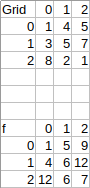
\includegraphics{minimum-path-sum.png}\\
\figcaption{Minimum Path Sum}\label{fig:minimum-path-sum}
\end{center}


\subsubsection{備忘錄法}
\begin{Code}
// LeetCode, Minimum Path Sum
// 備忘錄法
class Solution {
public:
    int minPathSum(vector<vector<int> > &grid) {
        const int m = grid.size();
        const int n = grid[0].size();
        this->f = vector<vector<int> >(m, vector<int>(n, -1));
        return dfs(grid, m-1, n-1);
    }
private:
    vector<vector<int> > f;  // 緩存

    int dfs(const vector<vector<int> > &grid, int x, int y) {
        if (x < 0 || y < 0) return INT_MAX; // 越界,終止條件,注意,不是0

        if (x == 0 && y == 0) return grid[0][0]; // 回到起點,收斂條件

        return min(getOrUpdate(grid, x - 1, y),
                getOrUpdate(grid, x, y - 1)) + grid[x][y];
    }

    int getOrUpdate(const vector<vector<int> > &grid, int x, int y) {
        if (x < 0 || y < 0) return INT_MAX; // 越界,注意,不是0
        if (f[x][y] >= 0) return f[x][y];
        else return f[x][y] = dfs(grid, x, y);
    }
};
\end{Code}


\subsubsection{動規}
\begin{Code}
// LeetCode, Minimum Path Sum
// 二維動規
class Solution {
public:
    int minPathSum(vector<vector<int> > &grid) {
        if (grid.size() == 0) return 0;
        const int m = grid.size();
        const int n = grid[0].size();

        int f[m][n];
        f[0][0] = grid[0][0];
        for (int i = 1; i < m; i++) {
            f[i][0] = f[i - 1][0] + grid[i][0];
        }
        for (int i = 1; i < n; i++) {
            f[0][i] = f[0][i - 1] + grid[0][i];
        }

        for (int i = 1; i < m; i++) {
            for (int j = 1; j < n; j++) {
                f[i][j] = min(f[i - 1][j], f[i][j - 1]) + grid[i][j];
            }
        }
        return f[m - 1][n - 1];
    }
};
\end{Code}


\subsubsection{動規+滾動數組}
\begin{Code}
// LeetCode, Minimum Path Sum
// 二維動規+滾動數組
class Solution {
public:
    int minPathSum(vector<vector<int> > &grid) {
        const int m = grid.size();
        const int n = grid[0].size();

        int f[n];
        fill(f, f+n, INT_MAX); // 初始值是 INT_MAX,因為後面用了min函數。
        f[0] = 0;

        for (int i = 0; i < m; i++) {
            f[0] += grid[i][0];
            for (int j = 1; j < n; j++) {
                // 左邊的f[j],表示更新後的f[j],與公式中的f[i[[j]對應
                // 右邊的f[j],表示老的f[j],與公式中的f[i-1][j]對應
                f[j] = min(f[j - 1], f[j]) + grid[i][j];
            }
        }
        return f[n - 1];
    }
};
\end{Code}

\subsubsection{相關題目}
\begindot
\item Unique Paths, 見 \S \ref{sec:unique-paths}
\item Unique Paths II, 見 \S \ref{sec:unique-paths-ii}
\myenddot


\section{Edit Distance} %%%%%%%%%%%%%%%%%%%%%%%%%%%%%%
\label{sec:edit-distance}


\subsubsection{描述}
Given two words \fn{word1} and \fn{word2}, find the minimum number of steps required to convert \fn{word1} to \fn{word2}. (each operation is counted as 1 step.)

You have the following 3 operations permitted on a word:
\begindot
\item Insert a character
\item Delete a character
\item Replace a character
\myenddot


\subsubsection{分析}
設狀態為\fn{f[i][j]},表示\fn{A[0,i]}和\fn{B[0,j]}之間的最小編輯距離。設\fn{A[0,i]}的形式是\fn{str1c},\fn{B[0,j]}的形式是\fn{str2d},
\begin{enumerate}
\item 如果\fn{c==d},則\fn{f[i][j]=f[i-1][j-1]};
\item 如果\fn{c!=d},
    \begin{enumerate}
        \item 如果將c替換成d,則\fn{f[i][j]=f[i-1][j-1]+1};
        \item 如果在c後面添加一個d,則\fn{f[i][j]=f[i][j-1]+1};
        \item 如果將c刪除,則\fn{f[i][j]=f[i-1][j]+1};
    \end{enumerate}
\end{enumerate}


\begin{center}
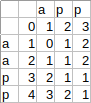
\includegraphics{edit-distance.png}\\
\figcaption{Edit Distance}\label{fig:edit-distance}
\end{center}

\subsubsection{動規}
\begin{Code}
// LeetCode, Edit Distance
// 二維動規,時間複雜度O(n*m),空間複雜度O(n*m)
class Solution {
public:
    int minDistance(const string &word1, const string &word2) {
        const size_t n = word1.size();
        const size_t m = word2.size();
        // 長度為n的字符串,有n+1個隔板
        int f[n + 1][m + 1];
        for (size_t i = 0; i <= n; i++)
            f[i][0] = i;
        for (size_t j = 0; j <= m; j++)
            f[0][j] = j;

        for (size_t i = 1; i <= n; i++) {
            for (size_t j = 1; j <= m; j++) {
                if (word1[i - 1] == word2[j - 1])
                    f[i][j] = f[i - 1][j - 1];
                else {
                    int mn = min(f[i - 1][j], f[i][j - 1]);
                    f[i][j] = 1 + min(f[i - 1][j - 1], mn);
                }
            }
        }
        return f[n][m];
    }
};
\end{Code}


\subsubsection{動規+滾動數組}
\begin{Code}
// LeetCode, Edit Distance
// 二維動規+滾動數組
// 時間複雜度O(n*m),空間複雜度O(n)
class Solution {
public:
    int minDistance(const string &word1, const string &word2) {
        if (word1.length() < word2.length())
            return minDistance(word2, word1);

        int f[word2.length() + 1];
        int upper_left = 0; // 額外用一個變量記錄f[i-1][j-1]

        for (size_t i = 0; i <= word2.size(); ++i)
            f[i] = i;

        for (size_t i = 1; i <= word1.size(); ++i) {
            upper_left = f[0];
            f[0] = i;

            for (size_t j = 1; j <= word2.size(); ++j) {
                int upper = f[j];

                if (word1[i - 1] == word2[j - 1])
                    f[j] = upper_left;
                else
                    f[j] = 1 + min(upper_left, min(f[j], f[j - 1]));

                upper_left = upper;
            }
        }

        return f[word2.length()];
    }
};
\end{Code}


\subsubsection{相關題目}
\begindot
\item 無
\myenddot


\section{Decode Ways} %%%%%%%%%%%%%%%%%%%%%%%%%%%%%%
\label{sec:decode-ways}


\subsubsection{描述}
A message containing letters from \fn{A-Z} is being encoded to numbers using the following mapping:
\begin{Code}
'A' -> 1
'B' -> 2
...
'Z' -> 26
\end{Code}

Given an encoded message containing digits, determine the total number of ways to decode it.

For example,
Given encoded message \fn{"12"}, it could be decoded as \fn{"AB"} (1 2) or \fn{"L"} (12).

The number of ways decoding \fn{"12"} is 2.


\subsubsection{分析}
跟 Climbing Stairs (見 \S \ref{sec:climbing-stairs})很類似,不過多加一些判斷邏輯。


\subsubsection{代碼}
\begin{Code}
// LeetCode, Decode Ways
// 動規,時間複雜度O(n),空間複雜度O(1)
class Solution {
public:
    int numDecodings(const string &s) {
        if (s.empty() || s[0] == '0') return 0;

        int prev = 0;
        int cur = 1;
        // 長度為n的字符串,有 n+1個階梯
        for (size_t i = 1; i <= s.size(); ++i) {
            if (s[i-1] == '0') cur = 0;

            if (i < 2 || !(s[i - 2] == '1' ||
                     (s[i - 2] == '2' && s[i - 1] <= '6')))
                prev = 0;

            int tmp = cur;
            cur = prev + cur;
            prev = tmp;
        }
        return cur;
    }
};
\end{Code}


\subsubsection{相關題目}
\begindot
\item Climbing Stairs, 見 \S \ref{sec:climbing-stairs}
\myenddot


\section{Distinct Subsequences} %%%%%%%%%%%%%%%%%%%%%%%%%%%%%%
\label{sec:distinct-subsequences}


\subsubsection{描述}
Given a string $S$ and a string $T$, count the number of distinct subsequences of $T$ in $S$.

A subsequence of a string is a new string which is formed from the original string by deleting some (can be none) of the characters without disturbing the relative positions of the remaining characters. (ie, \fn{"ACE"} is a subsequence of \fn{"ABCDE"} while \fn{"AEC"} is not).

Here is an example:
$S$ = \fn{"rabbbit"}, $T$ = \fn{"rabbit"}

Return 3.


\subsubsection{分析}
設狀態為$f(i,j)$,表示\fn{T[0,j]}在\fn{S[0,i]}裏出現的次數。首先,無論\fn{S[i]}和\fn{T[j]}是否相等,若不使用\fn{S[i]},則$f(i,j)=f(i-1,j)$;若\fn{S[i]==T[j]},則可以使用\fn{S[i]},此時$f(i,j)=f(i-1,j)+f(i-1, j-1)$。

\begin{center}
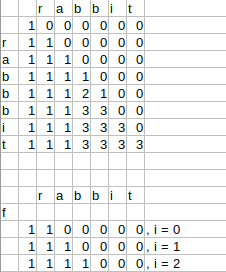
\includegraphics{distinct-subsequences.png}\\
\figcaption{Distinct Subsequences}\label{fig:distinct-subsequences}
\end{center}

\subsubsection{代碼}
\begin{Code}
// LeetCode, Distinct Subsequences
// 二維動規+滾動數組
// 時間複雜度O(m*n),空間複雜度O(n)
class Solution {
public:
    int numDistinct(const string &S, const string &T) {
        vector<int> f(T.size() + 1);
        f[0] = 1;
        for (int i = 0; i < S.size(); ++i) {
            for (int j = T.size() - 1; j >= 0; --j) {
                f[j + 1] += S[i] == T[j] ? f[j] : 0;
            }
        }

        return f[T.size()];
    }
};
\end{Code}


\subsubsection{相關題目}
\begindot
\item 無
\myenddot


\section{Word Break} %%%%%%%%%%%%%%%%%%%%%%%%%%%%%%
\label{sec:word-break}


\subsubsection{描述}
Given a string s and a dictionary of words dict, determine if s can be segmented into a space-separated sequence of one or more dictionary words.

For example, given \\
s = \fn{"leetcode"},\\
dict = \fn{["leet", "code"]}.

Return true because \fn{"leetcode"} can be segmented as \fn{"leet code"}.


\subsubsection{分析}
設狀態為$f(i)$,表示\fn{s[0,i]}是否可以分詞,則狀態轉移方程為
$$
f(i) = any\_of(f(j) \&\& s[j+1,i] \in dict),  0 \leq j < i
$$


\subsubsection{深搜}
\begin{Code}
// LeetCode, Word Break
// 深搜,超時
// 時間複雜度O(2^n),空間複雜度O(n)
class Solution {
public:
    bool wordBreak(string s, unordered_set<string> &dict) {
        return dfs(s, dict, 0, 0);
    }
private:
    static bool dfs(const string &s, unordered_set<string> &dict,
            size_t start, size_t cur) {
        if (cur == s.size()) {
            return dict.find(s.substr(start, cur-start+1)) != dict.end();
        }
        if (dfs(s, dict, start, cur+1)) return true;
        if (dict.find(s.substr(start, cur-start+1)) != dict.end())
            if (dfs(s, dict, cur+1, cur+1)) return true;
        return false;
    }
};
\end{Code}


\subsubsection{動規}
\begin{Code}
// LeetCode, Word Break
// 動規,時間複雜度O(n^2),空間複雜度O(n)
class Solution {
public:
    bool wordBreak(string s, unordered_set<string> &dict) {
        // 長度為n的字符串有n+1個隔板
        vector<bool> f(s.size() + 1, false);
        f[0] = true; // 空字符串
        for (int i = 1; i <= s.size(); ++i) {
            for (int j = i - 1; j >= 0; --j) {
                if (f[j] && dict.find(s.substr(j, i - j)) != dict.end()) {
                    f[i] = true;
                    break;
                }
            }
        }
        return f[s.size()];
    }
};
\end{Code}


\subsubsection{相關題目}
\begindot
\item Word Break II, 見 \S \ref{sec:word-break-ii}
\myenddot


\section{Word Break II} %%%%%%%%%%%%%%%%%%%%%%%%%%%%%%
\label{sec:word-break-ii}


\subsubsection{描述}
Given a string s and a dictionary of words dict, add spaces in s to construct a sentence where each word is a valid dictionary word.

Return all such possible sentences.

For example, given  \\
s = \fn{"catsanddog"}, \\
dict = \fn{["cat", "cats", "and", "sand", "dog"]}.

A solution is \fn{["cats and dog", "cat sand dog"]}.


\subsubsection{分析}
在上一題的基礎上,要返回解本身。


\subsubsection{代碼}
\begin{Code}
// LeetCode, Word Break II
// 動規,時間複雜度O(n^2),空間複雜度O(n^2)
class Solution {
public:
    vector<string> wordBreak(string s, unordered_set<string> &dict) {
        // 長度為n的字符串有n+1個隔板
        vector<bool> f(s.length() + 1, false);
        // prev[i][j]為true,表示s[j, i)是一個合法單詞,可以從j處切開
        // 第一行未用
        vector<vector<bool> > prev(s.length() + 1, vector<bool>(s.length()));
        f[0] = true;
        for (size_t i = 1; i <= s.length(); ++i) {
            for (int j = i - 1; j >= 0; --j) {
                if (f[j] && dict.find(s.substr(j, i - j)) != dict.end()) {
                    f[i] = true;
                    prev[i][j] = true;
                }
            }
        }
        vector<string> result;
        vector<string> path;
        gen_path(s, prev, s.length(), path, result);
        return result;

    }
private:
    // DFS遍歷樹,生成路徑
    void gen_path(const string &s, const vector<vector<bool> > &prev,
            int cur, vector<string> &path, vector<string> &result) {
        if (cur == 0) {
            string tmp;
            for (auto iter = path.crbegin(); iter != path.crend(); ++iter)
                tmp += *iter + " ";
            tmp.erase(tmp.end() - 1);
            result.push_back(tmp);
        }
        for (size_t i = 0; i < s.size(); ++i) {
            if (prev[cur][i]) {
                path.push_back(s.substr(i, cur - i));
                gen_path(s, prev, i, path, result);
                path.pop_back();
            }
        }
    }
};
\end{Code}


\subsubsection{相關題目}
\begindot
\item Word Break, 見 \S \ref{sec:word-break}
\myenddot

\chapter{圖}

無向圖的節點定義如下:
\begin{Code}
// 無向圖的節點
struct UndirectedGraphNode {
    int label;
    vector<UndirectedGraphNode *> neighbors;
    UndirectedGraphNode(int x) : label(x) {};
};
\end{Code}


\section{Clone Graph} %%%%%%%%%%%%%%%%%%%%%%%%%%%%%%
\label{sec:clone-graph}


\subsubsection{描述}
Clone an undirected graph. Each node in the graph contains a \code{label} and a list of its \code{neighbours}.


OJ's undirected graph serialization:
Nodes are labeled uniquely.

We use \code{\#} as a separator for each node, and \code{,} as a separator for node label and each neighbour of the node.
As an example, consider the serialized graph \code{\{0,1,2\#1,2\#2,2\}}.

The graph has a total of three nodes, and therefore contains three parts as separated by \code{\#}.
\begin{enumerate}
\item First node is labeled as 0. Connect node 0 to both nodes 1 and 2.
\item Second node is labeled as 1. Connect node 1 to node 2.
\item Third node is labeled as 2. Connect node 2 to node 2 (itself), thus forming a self-cycle.
\end{enumerate}

Visually, the graph looks like the following:
\begin{Code}
       1
      / \
     /   \
    0 --- 2
         / \
         \_/
\end{Code}


\subsubsection{分析}
廣度優先遍歷或深度優先遍歷都可以。


\subsubsection{DFS}
\begin{Code}
// LeetCode, Clone Graph
// DFS,時間複雜度O(n),空間複雜度O(n)
class Solution {
public:
    UndirectedGraphNode *cloneGraph(const UndirectedGraphNode *node) {
        if(node == nullptr) return nullptr;
        // key is original node,value is copied node
        unordered_map<const UndirectedGraphNode *,
                            UndirectedGraphNode *> copied;
        clone(node, copied);
        return copied[node];
    }
private:
    // DFS
    static UndirectedGraphNode* clone(const UndirectedGraphNode *node,
            unordered_map<const UndirectedGraphNode *,
            UndirectedGraphNode *> &copied) {
        // a copy already exists
        if (copied.find(node) != copied.end()) return copied[node];

        UndirectedGraphNode *new_node = new UndirectedGraphNode(node->label);
        copied[node] = new_node;
        for (auto nbr : node->neighbors)
            new_node->neighbors.push_back(clone(nbr, copied));
        return new_node;
    }
};
\end{Code}


\subsubsection{BFS}
\begin{Code}
// LeetCode, Clone Graph
// BFS,時間複雜度O(n),空間複雜度O(n)
class Solution {
public:
    UndirectedGraphNode *cloneGraph(const UndirectedGraphNode *node) {
        if (node == nullptr) return nullptr;
        // key is original node,value is copied node
        unordered_map<const UndirectedGraphNode *,
                            UndirectedGraphNode *> copied;
        // each node in queue is already copied itself
        // but neighbors are not copied yet
        queue<const UndirectedGraphNode *> q;
        q.push(node);
        copied[node] = new UndirectedGraphNode(node->label);
        while (!q.empty()) {
            const UndirectedGraphNode *cur = q.front();
            q.pop();
            for (auto nbr : cur->neighbors) {
                // a copy already exists
                if (copied.find(nbr) != copied.end()) {
                    copied[cur]->neighbors.push_back(copied[nbr]);
                } else {
                    UndirectedGraphNode *new_node =
                            new UndirectedGraphNode(nbr->label);
                    copied[nbr] = new_node;
                    copied[cur]->neighbors.push_back(new_node);
                    q.push(nbr);
                }
            }
        }
        return copied[node];
    }
};
\end{Code}


\subsubsection{相關題目}
\begindot
\item 無
\myenddot

\section{Network Delay Time} %%%%%%%%%%%%%%%%%%%%%%%%%%%%%%
\label{sec:network-delay-time}


\subsubsection{描述}
There are N network nodes, labelled 1 to N.

Given times, a list of travel times as directed edges times[i] = (u, v, w), where u is the source node, v is the target node, and w is the time it takes for a signal to travel from source to target.

Now, we send a signal from a certain node K. How long will it take for all nodes to receive the signal? If it is impossible, return -1.

\begin{center}
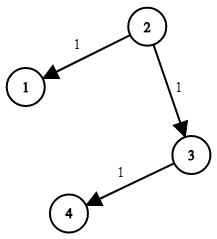
\includegraphics[width=100pt]{network-delay-time.png}\\
\figcaption{Rotate Image}\label{fig:network-delay-time}
\end{center}

\begin{Code}
Input: times = [[2,1,1],[2,3,1],[3,4,1]], N = 4, K = 2
Output: 2
\end{Code}

\begin{enumerate}
\item N will be in the range [l, 100]
\item K will be in the range [l, N]
\item The length of times will be in the range [l, 6000].
\item All edges times[i] = (u, v, w) will have l <= u, v <= N and 0 <= w <= 100.
\end{enumerate}
\subsubsection{分析}
廣度優先遍歷
Use Djikstra Algorithm. Find a minium path from one source to one end.


\subsubsection{Djikstra}
\begin{Code}
// LeetCode, Clone Graph
// DFS with graph,時間複雜度O(ELogV),空間複雜度O(V^2)
class Solution {
public:
    struct Node {
        int m_node;
        int m_dist;

        Node (int node, int dist)
            : m_node(node), m_dist(dist) {}
    };
    int networkDelayTime(vector<vector<int>>& times, int N, int K) {
        // create graph
        unordered_map<int, list<Node>> graph;  // key: nodeNumber value: nodes
        for (const auto& t : times) // startNode: t[0], endNode: t[1], dist: t[2]
            graph[t[0]].push_back(Node(t[1], t[2]));

        unordered_map<int, int> dist; // key: nodeNumber value: dist
        multimap<int, int> dq; // djikstra queue, key: dist value: nodeNumber

        // do until no more node in queue
        dq.insert(make_pair(0, K));
        while (!dq.empty()) {
            pair<int, int> cur = *dq.begin();
            dq.erase(dq.begin());

            // filter out if shortest path is found
            if (dist.find(cur.second) != dist.end()) continue;
            // record the shortest parth
            dist.insert(make_pair(cur.second, cur.first));
            // push the neighbour to dq
            auto it = graph.find(cur.second);
            if (it == graph.end()) continue;
            for (const auto& nei : it->second) {
                if (dist.find(nei.m_node) != dist.end()) continue;
                dq.insert(make_pair(nei.m_dist + cur.first, nei.m_node));
            }
        }

        // pick the max dist, return -1 if not all node is visited
        if ((int)dist.size() == N)
            return max_element(dist.begin(), dist.end()
              , [&](const pair<int, int>& first, const pair<int, int>& second)
                                {
                                    return first.second < second.second;
                                })->second;
        else
            return -1;
    }
};

\end{Code}
\subsubsection{Djikstra}
\begin{Code}
// LeetCode, Clone Graph
// DFS with adjacency list,時間複雜度O(ELogV),空間複雜度O(V^2)
class Solution {
public:
    int networkDelayTime(vector<vector<int>>& times, int N, int K)
    {
        // Build adjacency list
        // index 0 is dummy for easy implementation
        vector<vector<pair<int, int>>> adjList(N + 1);
        for (const auto& v : times)
            adjList[v[0]].emplace_back(v[1], v[2]);

        vector<int> dist(N + 1, INT_MAX);
        // initialize pq and source vertex distance
        dist[K] = 0;
        set<pair<int, int>> pq {{dist[K], K}};
        while (!pq.empty()) {
            const auto u = pq.begin()->second;
            pq.erase(pq.begin()); // pop the top, i.e., first element in set
            for (const auto& [v, w]: adjList[u]) {
                if (dist[u] + w < dist[v]) { // if edge can be relaxed
                    pq.erase({dist[v], v}); // remove old info
                    dist[v] = dist[u] + w;  // update distance
                    pq.emplace(dist[v], v); // insert new info
                }
            }
        }

        const int longestTime = *max_element(dist.begin() + 1, dist.end());
        return longestTime == INT_MAX ? -1 : longestTime;
    }
};
\end{Code}

\subsubsection{相關題目}
\begindot
\item 無
\myenddot

\section{Alien Dictionary} %%%%%%%%%%%%%%%%%%%%%%%%%%%%%%
\label{sec:alien-dictionary}

\subsubsection{描述}
There is a new alien language which uses the latin alphabet. However, the order among letters are unknown to you. You receive a list of non-empty words from the dictionary, where words are sorted lexicographically by the rules of this new language. Derive the order of letters in this language.

Example 1:
\begin{Code}
Input:
[
  "wrt",
  "wrf",
  "er",
  "ett",
  "rftt"
]

Output: "wertf"
\end{Code}

Example 2:
\begin{Code}
Input:
[
  "z",
  "x"
]

Output: "zx"
\end{Code}

Example 3:
\begin{Code}
Input:
[
  "z",
  "x",
  "z"
] 

Output: "" 
\end{Code}

\subsubsection{分析}
Make DAG from sorted strings, do topological sort by BFS or DFS


\subsubsection{BFS with List}
\begin{Code}
// LeetCode, Alien Dictionary
// BFS Topological sort,時間複雜度O(N),空間複雜度O(N)
class Solution {
public:
    string alienOrder(vector<string>& words) {
        unordered_map<char, list<char>> adjList; // 用來記低依賴關係
        unordered_map<char, int> depenCount; // 用來儲存每個字母的依賴數目

        for (const auto& w : words)
            for (const auto& c : w)
            {
                depenCount[c] = 0;
                adjList.insert(make_pair(c, list<char>()));
            }
        // 製造 adjList DAG
        for (size_t i = 0; i < words.size() - 1; i++)
        {
            const string& w1 = words[i];
            const string& w2 = words[i+1];
            // 剪枝,若 prefix 一樣
            if (w1.size() > w2.size() && w1.find(w2) == 0) return "";
            // 找尋第一個不同的字母
            for (size_t j = 0; j < w1.size() && j < w2.size(); j++)
            {
                const char& c1 = w1[j];
                const char& c2 = w2[j];
                if (c1 != c2)
                {
                    adjList[c1].push_back(c2);
                    depenCount[c2]++;
                    break;
                }
            }
        }
        // 利用 Topological Sort 來解決相關的依賴關係
        queue<char> cur;
        // 先處理沒有依賴的字母
        for (const auto& [k, v] : depenCount)
            if (v == 0)
                cur.push(k);

        string result;
        // BFS
        while (!cur.empty())
        {
            char c = cur.front();
            cur.pop();
            result.push_back(c);
            auto it = adjList.find(c);
            if (it == adjList.end()) continue;
            for (const auto& nei : it->second)
            {
                if (--(depenCount[nei]) == 0)
                    cur.push(nei);
            }
        }

        if (result.size() < depenCount.size())
            return "";
        else
            return result;
    }
};
\end{Code}

\subsubsection{BFS with Set}
\begin{Code}
// LeetCode, Alien Dictionary
// BFS Topological sort,時間複雜度O(N),空間複雜度O(N)
class Solution {
public:
    string alienOrder(vector<string>& words) {
        unordered_map<char, set<char>> adjList; // 用來記低依賴關係
        unordered_map<char, int> depenCount; // 用來儲存每個字母的依賴數目

        for (const auto& w : words)
            for (const auto& c : w)
            {
                depenCount[c] = 0;
                adjList.insert(make_pair(c, set<char>()));
            }
        // 製造 adjList DAG
        for (size_t i = 0; i < words.size() - 1; i++)
        {
            const string& w1 = words[i];
            const string& w2 = words[i+1];
            // 剪枝,若 prefix 一樣
            if (w1.size() > w2.size() && w1.find(w2) == 0) return "";
            // 找尋第一個不同的字母
            for (size_t j = 0; j < w1.size() && j < w2.size(); j++)
            {
                const char& c1 = w1[j];
                const char& c2 = w2[j];
                if (c1 != c2)
                {
                    if (adjList[c1].find(c2) == adjList[c1].end()) // 這裏不同
                    {
                        adjList[c1].insert(c2);
                        depenCount[c2]++;
                    }
                    break;
                }
            }
        }
        // 之後的動作和上一個例子一樣,略去 。。。 //
    }
};

\end{Code}

\subsubsection{DFS with List}
\begin{Code}
// LeetCode, Alien Dictionary
// DFS Topological sort,時間複雜度O(N),空間複雜度O(N)
class Solution {
public:
    string alienOrder(vector<string>& words) {
        unordered_map<char, list<char>> adjList; // 用來記低依賴關係
        
        // 製造 DAG,令到所有字母也有被歷篇的機會
        for (const auto& w : words)
            for (const auto& c : w)
                adjList.insert(make_pair(c, list<char>()));
        // 製造剩下的 DAG
        for (size_t i = 0; i < words.size() - 1; i++)
        {
            const string& w1 = words[i];
            const string& w2 = words[i+1];
            // 找到 prefix case
            if (w1.size() > w2.size() && w1.find(w2) == 0) return "";
            
            for (size_t j = 0; j < w1.size() && j < w2.size(); j++)
            {
                const char& c1 = w1[j];
                const char& c2 = w2[j];
                if (c1 != c2)
                {
                    adjList[c1].push_back(c2);
                    break;
                }
            }
        }
        
        string result;
        unordered_map<char, bool> visited;
        for (const auto& [k, v] : adjList)
        {
            if (!DFS(adjList, visited, k, result))
                return "";
        }
        
        if (result.size() < adjList.size())
            return "";
        else
            return result;
    }
private:
    bool DFS(unordered_map<char, list<char>>& adjList, unordered_map<char, bool>& visited, char k, string& result)
    {
        if (visited.find(k) != visited.end())
            return visited[k]; // If this node was grey (false), a cycle was detected.
        
        visited[k] = false;
        auto it = adjList.find(k);
        for (const auto& nei : adjList[k])
        {
            if (!DFS(adjList, visited, *nei, result)) return false;
        }
        visited[k] = true;
        result.insert(result.begin(), k);
        
        return true;
    }
};

\end{Code}

\subsubsection{相關題目}
\begindot
\item Topological sort,見 \S \ref{sec:topological-sort}
\myenddot

\section{Redundant Connection} %%%%%%%%%%%%%%%%%%%%%%%%%%%%%%
\label{sec:redundant-connection}

\subsubsection{描述}
In this problem, a tree is an undirected graph that is connected and has no cycles.

The given input is a graph that started as a tree with N nodes (with distinct values 1, 2, ..., N), with one additional edge added. The added edge has two different vertices chosen from 1 to N, and was not an edge that already existed.

The resulting graph is given as a 2D-array of edges. Each element of edges is a pair [u, v] with u < v, that represents an undirected edge connecting nodes u and v.

Return an edge that can be removed so that the resulting graph is a tree of N nodes. If there are multiple answers, return the answer that occurs last in the given 2D-array. The answer edge [u, v] should be in the same format, with u < v.


Example 1:
\begin{Code}
Input: [[1,2], [1,3], [2,3]]
Output: [2,3]
Explanation: The given undirected graph will be like this:
  1
 / \
2 - 3
\end{Code}

Example 2:
\begin{Code}
Input: [[1,2], [2,3], [3,4], [1,4], [1,5]]
Output: [1,4]
Explanation: The given undirected graph will be like this:
5 - 1 - 2
    |   |
    4 - 3
\end{Code}


Note:
\begindot
\item The size of the input 2D-array will be between 3 and 1000.
\item Every integer represented in the 2D-array will be between 1 and N, where N is the size of the input array.
\myenddot


\subsubsection{DFS}
\begin{Code}
// 時間複雜度O(N^2),空間複雜度O(N)
// 重點:當發現有多過一個路徑可由 u 走到 v,便發現答案
class Solution {
public:
    vector<int> findRedundantConnection(vector<vector<int>>& edges) {
        // 記低見過的 edges, 由 u -> v
        unordered_map<int, unordered_set<int>> cache;

        for (const auto& edge : edges)
        {
            const int& u = edge[0];
            const int& v = edge[1];
            // 利用 DFS 來驗證有沒有另一個方法可以由 u 跑到 v
            unordered_set<int> visited;
            if (cache.count(u) && cache.count(v) && DFS(cache, visited, u, v))
                return vector<int>{u, v};

            cache[u].insert(v);
            cache[v].insert(u);
        }

        return vector<int>();
    }
private:
    template <class eMap, class Vis>
        bool DFS(eMap& cache, Vis& visited, const int& start, const int& target)
    {
        if (start == target) return true;

        if (cache.find(start) == cache.end()) return false;

        visited.insert(start);
        for (const int& nei : cache[start])
            if (!visited.count(nei) && DFS(cache, visited, nei, target))
                return true;

        return false;
    }
};
\end{Code}

\subsubsection{DSU - Without Rank}
\begin{Code}
// 時間複雜度O(N),空間複雜度O(N)
// 一開始每個點都以自己為一個集合(set)
// 歷遍所有 edge,把點放於同一個集合。
// 若果兩點早已是同一集合,那個 edge 便是多餘。
// https://www.youtube.com/watch?time_continue=1124&v=wU6udHRIkcc&feature=emb_title
class DSU // Disjoint Set Union (DSU)
{
public:
    DSU(int N)
    {
        m_parent.reserve(N);
        for (int i = 0; i < N; i++) m_parent.push_back(i);
    }
    ~DSU() {}

    int FindParent(const int& x)
    {
        if (m_parent[x] == x) // 當 x 為集合的父親時
            return x;
        return m_parent[x] = FindParent(m_parent[x]); // x 的集合等如 x 的父親的集合
    }
    bool Union(const int& x, const int& y)
    {
        const int xpar = FindParent(x);
        const int ypar = FindParent(y);
        if (xpar == ypar) return false;

        m_parent[xpar] = ypar; // perform union

        return true;
    }
private:
    vector<int> m_parent; // 利用數列來記低點的所在集合
};
class Solution
{
public:
    vector<int> findRedundantConnection(vector<vector<int>>& edges) {
        DSU dsu(1001);

        for (const auto& edge : edges)
        {
            const int& u = edge[0];
            const int& v = edge[1];

            if (!dsu.Union(u, v))
                return vector<int>{u, v};
        }

        return vector<int>();
    }
};
\end{Code}

\subsubsection{DSU - Rank}
\begin{Code}
// 時間複雜度O(N),空間複雜度O(N)
// 一開始每個點都以自己為一個集合(set)
// 歷遍所有 edge,把點放於同一個集合。
// 若果兩點早已是同一集合,那個 edge 便是多餘。
class DSU // Disjoint Set Union (DSU)
{
public:
    DSU(int N)
    {
        // 負數意指該合集的父親
        // 所以一開始,每個點都是某個合集的父親
        // 負數的值代表 rank, 也是該合集的點的總數
        // 正數的值代表父的 index
        m_parent.resize(N, -1);
    }
    ~DSU() {}

    int FindParent(const int& x)
    {
        if (m_parent[x] < 0)
            return x;
        return m_parent[x] = FindParent(m_parent[x]);
    }
    bool Union(const int& x, const int& y)
    {
        const int xpar = FindParent(x);
        const int ypar = FindParent(y);
        if (xpar == ypar) return false;

        if (abs(m_parent[xpar]) < abs(m_parent[ypar]))
        {
            m_parent[ypar] += m_parent[xpar];
            m_parent[xpar] = ypar;
        }
        else
        {
            m_parent[xpar] += m_parent[ypar];
            m_parent[ypar] = xpar;
        }

        return true;
    }
private:
    vector<int> m_parent;
};
class Solution {
public:
    vector<int> findRedundantConnection(vector<vector<int>>& edges) {
        DSU dsu(1001);

        for (const auto& edge : edges)
        {
            const int& u = edge[0];
            const int& v = edge[1];

            if (!dsu.Union(u, v))
                return vector<int>{u, v};
        }

        return vector<int>();
    }
};
\end{Code}

\chapter{細節實現題}
這類題目不考特定的算法,純粹考察寫代碼的熟練度。
\newline


\section{Reverse Integer} %%%%%%%%%%%%%%%%%%%%%%%%%%%%%%
\label{sec:reverse-integer}


\subsubsection{描述}
Reverse digits of an integer.

Example1: x = 123, return 321

Example2: x = -123, return -321


\textbf{Have you thought about this?}

Here are some good questions to ask before coding. Bonus points for you if you have already thought through this!

If the integer's last digit is 0, what should the output be? ie, cases such as 10, 100.

Did you notice that the reversed integer might overflow? Assume the input is a 32-bit integer, then the reverse of 1000000003 overflows. How should you handle such cases?

Throw an exception? Good, but what if throwing an exception is not an option? You would then have to re-design the function (ie, add an extra parameter).


\subsubsection{分析}
短小精悍的題,代碼也可以寫的很短小。


\subsubsection{代碼}
\begin{Code}
//LeetCode, Reverse Integer
// 時間複雜度O(logn),空間複雜度O(1)
// 考慮 1.負數的情況 2. 溢出的情況(正溢出&&負溢出,比如 x = -2147483648(即-2^31) )
class Solution {
public:
    int reverse (int x) {
        long long r = 0;
        long long t = x;
        t = t > 0 ? t : -t;
        for (; t; t /= 10)
            r = r * 10 + t % 10;

        bool sign = x > 0 ? false: true;
        if (r > 2147483647 || (sign && r > 2147483648)) {
            return 0;
        } else {
            if (sign) {
                return -r;
            } else {
                return r;
            }
        }
    }
};
\end{Code}


\subsubsection{相關題目}
\begindot
\item Palindrome Number, 見 \S \ref{sec:palindrome-number}
\myenddot


\section{Palindrome Number} %%%%%%%%%%%%%%%%%%%%%%%%%%%%%%
\label{sec:palindrome-number}


\subsubsection{描述}
Determine whether an integer is a palindrome. Do this without extra space.

\textbf{Some hints:}

Could negative integers be palindromes? (ie, -1)

If you are thinking of converting the integer to string, note the restriction of using extra space.

You could also try reversing an integer. However, if you have solved the problem "Reverse Integer", you know that the reversed integer might overflow. How would you handle such case?

There is a more generic way of solving this problem.


\subsubsection{分析}
首先想到,可以利用上一題,將整數反轉,然後與原來的整數比較,是否相等,相等則為 Palindrome 的。可是 reverse()會溢出。

正確的解法是,不斷地取第一位和最後一位(10進制下)進行比較,相等則取第二位和倒數第二位,直到完成比較或者中途找到了不一致的位。


\subsubsection{代碼}
\begin{Code}
//LeetCode, Palindrome Number
// 時間複雜度O(1),空間複雜度O(1)
class Solution {
public:
    bool isPalindrome(int x) {
        if (x < 0) return false;
        int d = 1; // divisor
        while (x / d >= 10) d *= 10;

        while (x > 0) {
            int q = x / d;  // quotient
            int r = x % 10;   // remainder
            if (q != r) return false;
            x = x % d / 10;
            d /= 100;
        }
        return true;
    }
};
\end{Code}


\subsubsection{相關題目}
\begindot
\item Reverse Integer, 見 \S \ref{sec:reverse-integer}
\item Valid Palindrome, 見 \S \ref{sec:valid-palindrome}
\myenddot


\section{Insert Interval} %%%%%%%%%%%%%%%%%%%%%%%%%%%%%%
\label{sec:insert-interval}


\subsubsection{描述}
Given a set of non-overlapping intervals, insert a new interval into the intervals (merge if necessary).

You may assume that the intervals were initially sorted according to their start times.

Example 1:
Given intervals \code\{[1,3],[6,9]\}, insert and merge \code\{[2,5]\} in as \code\{[1,5],[6,9]\}.

Example 2:
Given \code\{[1,2],[3,5],[6,7],[8,10],[12,16]\}, insert and merge \code\{[4,9]\} in as \code\{[1,2],[3,10],[12,16]\}.

This is because the new interval \code\{[4,9]\} overlaps with \code\{[3,5],[6,7],[8,10]\}.


\subsubsection{分析}
無


\subsubsection{代碼}
\begin{Code}
struct Interval {
    int start;
    int end;
    Interval() : start(0), end(0) { }
    Interval(int s, int e) : start(s), end(e) { }
};

//LeetCode, Insert Interval
// 時間複雜度O(n),空間複雜度O(1)
class Solution {
public:
    vector<Interval> insert(vector<Interval> &intervals, Interval newInterval) {
        vector<Interval>::iterator it = intervals.begin();
        while (it != intervals.end()) {
            if (newInterval.end < it->start) {
                intervals.insert(it, newInterval);
                return intervals;
            } else if (newInterval.start > it->end) {
                it++;
                continue;
            } else {
                newInterval.start = min(newInterval.start, it->start);
                newInterval.end = max(newInterval.end, it->end);
                it = intervals.erase(it);
            }
        }
        intervals.insert(intervals.end(), newInterval);
        return intervals;
    }
};
\end{Code}


\subsubsection{相關題目}

\begindot
\item Merge Intervals,見 \S \ref{sec:merge-intervals}
\myenddot


\section{Merge Intervals} %%%%%%%%%%%%%%%%%%%%%%%%%%%%%%
\label{sec:merge-intervals}


\subsubsection{描述}
Given a collection of intervals, merge all overlapping intervals.

For example,
Given \code\{[1,3],[2,6],[8,10],[15,18]\},
return \code\{[1,6],[8,10],[15,18]\}


\subsubsection{分析}
複用一下Insert Intervals的解法即可,創建一個新的interval集合,然後每次從舊的裏面取一個interval出來,然後插入到新的集合中。


\subsubsection{代碼}
\begin{Code}
struct Interval {
    int start;
    int end;
    Interval() : start(0), end(0) { }
    Interval(int s, int e) : start(s), end(e) { }
};

//LeetCode, Merge Interval
//複用一下Insert Intervals的解法即可
// 時間複雜度O(n1+n2+...),空間複雜度O(1)
class Solution {
public:
    vector<Interval> merge(vector<Interval> &intervals) {
        vector<Interval> result;
        for (int i = 0; i < intervals.size(); i++) {
            insert(result, intervals[i]);
        }
        return result;
    }
private:
    vector<Interval> insert(vector<Interval> &intervals, Interval newInterval) {
        vector<Interval>::iterator it = intervals.begin();
        while (it != intervals.end()) {
            if (newInterval.end < it->start) {
                intervals.insert(it, newInterval);
                return intervals;
            } else if (newInterval.start > it->end) {
                it++;
                continue;
            } else {
                newInterval.start = min(newInterval.start, it->start);
                newInterval.end = max(newInterval.end, it->end);
                it = intervals.erase(it);
            }
        }
        intervals.insert(intervals.end(), newInterval);
        return intervals;
    }
};
\end{Code}
\subsubsection{代碼}
\begin{Code}
//LeetCode, Merge Interval
// Sort it and always push back into a reserved vector
// 時間複雜度O(nlogn),空間複雜度O(n)
class Solution {
public:
    vector<vector<int>> merge(vector<vector<int>>& intervals) {
        // sort it first
        sort(intervals.begin(), intervals.end(), [&](const auto& first, const auto& second)
             {
                return first[0] < second[0];
             });
        vector<vector<int>> result;
        result.reserve(intervals.size());

        for (const auto& interval : intervals)
            mergeBack(result, interval);

        return result;
    }
private:
    void mergeBack(vector<vector<int>>& result, const vector<int>& interval) {
        if (result.size() == 0) result.push_back(interval);

        int& start = result.back()[0];
        int& end = result.back()[1];

        if (interval[0] >= start && interval[0] <= end)
            end = max(end, interval[1]);
        else
            result.push_back(interval);
    }
};
\end{Code}


\subsubsection{相關題目}

\begindot
\item Insert Interval,見 \S \ref{sec:insert-interval}
\myenddot


\section{Minimum Window Substring} %%%%%%%%%%%%%%%%%%%%%%%%%%%%%%
\label{sec:minimum-window-substring}


\subsubsection{描述}
Given a string $S$ and a string $T$, find the minimum window in $S$ which will contain all the characters in $T$ in complexity $O(n)$.

For example, \code{S = "ADOBECODEBANC", T = "ABC"}

Minimum window is \code{"BANC"}.

Note:
\begindot
\item If there is no such window in $S$ that covers all characters in $T$, return the emtpy string \code{""}.
\item If there are multiple such windows, you are guaranteed that there will always be only one unique minimum window in $S$.
\myenddot


\subsubsection{分析}
雙指針,動態維護一個區間。尾指針不斷往後掃,當掃到有一個窗口包含了所有$T$的字符後,然後再收縮頭指針,直到不能再收縮為止。最後記錄所有可能的情況中窗口最小的


\subsubsection{代碼}
\begin{Code}
// LeetCode, Minimum Window Substring
// 時間複雜度O(n),空間複雜度O(1)
class Solution {
public:
    string minWindow(string S, string T) {
        if (S.empty()) return "";
        if (S.size() < T.size()) return "";

        const int ASCII_MAX = 256;
        int appeared_count[ASCII_MAX];
        int expected_count[ASCII_MAX];
        fill(appeared_count, appeared_count + ASCII_MAX, 0);
        fill(expected_count, expected_count + ASCII_MAX, 0);

        for (size_t i = 0; i < T.size(); i++) expected_count[T[i]]++;

        int minWidth = INT_MAX, min_start = 0;  // 窗口大小,起點
        int wnd_start = 0;
        int appeared = 0;  // 完整包含了一個T
        //尾指針不斷往後掃
        for (size_t wnd_end = 0; wnd_end < S.size(); wnd_end++) {
            if (expected_count[S[wnd_end]] > 0)  {  // this char is a part of T
                appeared_count[S[wnd_end]]++;
                if (appeared_count[S[wnd_end]] <= expected_count[S[wnd_end]])
                    appeared++;
            }
            if (appeared == T.size()) {  // 完整包含了一個T
                // 收縮頭指針
                while (appeared_count[S[wnd_start]] > expected_count[S[wnd_start]]
                        || expected_count[S[wnd_start]] == 0) {
                    appeared_count[S[wnd_start]]--;
                    wnd_start++;
                }
                if (minWidth > (wnd_end - wnd_start + 1)) {
                    minWidth = wnd_end - wnd_start + 1;
                    min_start = wnd_start;
                }
            }
        }

        if (minWidth == INT_MAX) return "";
        else return S.substr(min_start, minWidth);
    }
};
\end{Code}


\subsubsection{相關題目}

\begindot
\item 無
\myenddot


\section{Multiply Strings} %%%%%%%%%%%%%%%%%%%%%%%%%%%%%%
\label{sec:multiply-strings}


\subsubsection{描述}
Given two numbers represented as strings, return multiplication of the numbers as a string.

Note: The numbers can be arbitrarily large and are non-negative.


\subsubsection{分析}
高精度乘法。

常見的做法是將字符轉化為一個int,一一對應,形成一個int數組。但是這樣很浪費空間,一個int32的最大值是$2^{31}-1=2147483647$,可以與9個字符對應,由於有乘法,減半,則至少可以與4個字符一一對應。一個int64可以與9個字符對應。


\subsubsection{代碼1}
\begin{Code}
// LeetCode, Multiply Strings
// @author 連城 (http://weibo.com/lianchengzju)
// 一個字符對應一個int
// 時間複雜度O(n*m),空間複雜度O(n+m)
typedef vector<int> bigint;

bigint make_bigint(string const& repr) {
    bigint n;
    transform(repr.rbegin(), repr.rend(), back_inserter(n),
            [](char c) { return c - '0'; });
    return n;
}

string to_string(bigint const& n) {
    string str;
    transform(find_if(n.rbegin(), prev(n.rend()),
            [](char c) { return c > '\0'; }), n.rend(), back_inserter(str),
            [](char c) { return c + '0'; });
    return str;
}

bigint operator*(bigint const& x, bigint const& y) {
    bigint z(x.size() + y.size());

    for (size_t i = 0; i < x.size(); ++i)
        for (size_t j = 0; j < y.size(); ++j) {
            z[i + j] += x[i] * y[j];
            z[i + j + 1] += z[i + j] / 10;
            z[i + j] %= 10;
        }

    return z;
}

class Solution {
public:
    string multiply(string num1, string num2) {
        return to_string(make_bigint(num1) * make_bigint(num2));
    }
};
\end{Code}


\subsubsection{代碼2}
\begin{Code}
// LeetCode, Multiply Strings
// 9個字符對應一個int64_t
// 時間複雜度O(n*m/81),空間複雜度O((n+m)/9)
/** 大整數類. */
class BigInt {
public:
    /**
     * @brief 構造函數,將字符串轉化為大整數.
     * @param[in] s 輸入的字符串
     * @return 無
     */
    BigInt(string s) {
        vector<int64_t> result;
        result.reserve(s.size() / RADIX_LEN + 1);

        for (int i = s.size(); i > 0; i -= RADIX_LEN) {  // [i-RADIX_LEN, i)
            int temp = 0;
            const int low = max(i - RADIX_LEN, 0);
            for (int j = low; j < i; j++) {
                temp = temp * 10 + s[j] - '0';
            }
            result.push_back(temp);
        }
        elems = result;
    }
    /**
     * @brief 將整數轉化為字符串.
     * @return 字符串
     */
    string toString() {
        stringstream result;
        bool started = false; // 用於跳過前導0
        for (auto i = elems.rbegin(); i != elems.rend(); i++) {
            if (started) { // 如果多餘的0已經都跳過,則輸出
                result << setw(RADIX_LEN) << setfill('0') << *i;
            } else {
                result << *i;
                started = true; // 碰到第一個非0的值,就説明多餘的0已經都跳過
            }
        }

        if (!started) return "0"; // 當x全為0時
        else return result.str();
    }

    /**
     * @brief 大整數乘法.
     * @param[in] x x
     * @param[in] y y
     * @return 大整數
     */
    static BigInt multiply(const BigInt &x, const BigInt &y) {
        vector<int64_t> z(x.elems.size() + y.elems.size(), 0);

        for (size_t i = 0; i < y.elems.size(); i++) {
            for (size_t j = 0; j < x.elems.size(); j++) { // 用y[i]去乘以x的各位
                //  兩數第i, j位相乘,累加到結果的第i+j位
                z[i + j] += y.elems[i] * x.elems[j];

                if (z[i + j] >= BIGINT_RADIX) { //  看是否要進位
                    z[i + j + 1] += z[i + j] / BIGINT_RADIX; //  進位
                    z[i + j] %= BIGINT_RADIX;
                }
            }
        }
        while (z.back() == 0) z.pop_back();  // 沒有進位,去掉最高位的0
        return BigInt(z);
    }

private:
    typedef long long int64_t;
    /** 一個數組元素對應9個十進制位,即數組是億進制的
     * 因為 1000000000 * 1000000000 沒有超過 2^63-1
     */
    const static int BIGINT_RADIX = 1000000000;
    const static int RADIX_LEN = 9;
    /** 萬進制整數. */
    vector<int64_t> elems;
    BigInt(const vector<int64_t> num) : elems(num) {}
};


class Solution {
public:
    string multiply(string num1, string num2) {
        BigInt x(num1);
        BigInt y(num2);
        return BigInt::multiply(x, y).toString();
    }
};
\end{Code}


\subsubsection{相關題目}

\begindot
\item 無
\myenddot


\section{Substring with Concatenation of All Words} %%%%%%%%%%%%%%%%%%%%%%%%%%%%%%
\label{sec:substring-with-concatenation-of-all-words}


\subsubsection{描述}
You are given a string, $S$, and a list of words, $L$, that are all of the same length. Find all starting indices of substring(s) in $S$ that is a concatenation of each word in $L$ exactly once and without any intervening characters.

For example, given:
\begin{Code}
S: "barfoothefoobarman"
L: ["foo", "bar"]
\end{Code}

You should return the indices: \code\{[0,9]\}.(order does not matter).


\subsubsection{分析}
無


\subsubsection{代碼}
\begin{Code}
// LeetCode, Substring with Concatenation of All Words
// 時間複雜度O(n*m),空間複雜度O(m)
class Solution {
public:
    vector<int> findSubstring(string s, vector<string>& dict) {
        size_t wordLength = dict.front().length();
        size_t catLength = wordLength * dict.size();
        vector<int> result;

        if (s.length() < catLength) return result;

        unordered_map<string, int> wordCount;

        for (auto const& word : dict) ++wordCount[word];

        for (auto i = begin(s); i <= prev(end(s), catLength); ++i) {
            unordered_map<string, int> unused(wordCount);

            for (auto j = i; j != next(i, catLength); j += wordLength) {
                auto pos = unused.find(string(j, next(j, wordLength)));

                if (pos == unused.end() || pos->second == 0) break;

                if (--pos->second == 0) unused.erase(pos);
            }

            if (unused.size() == 0) result.push_back(distance(begin(s), i));
        }

        return result;
    }
};
\end{Code}


\subsubsection{相關題目}

\begindot
\item 無
\myenddot


\section{Pascal's Triangle} %%%%%%%%%%%%%%%%%%%%%%%%%%%%%%
\label{sec:pascal-s-triangle}


\subsubsection{描述}
Given $numRows$, generate the first $numRows$ of Pascal's triangle.

For example, given $numRows = 5$,

Return
\begin{Code}
[
     [1],
    [1,1],
   [1,2,1],
  [1,3,3,1],
 [1,4,6,4,1]
]
\end{Code}


\subsubsection{分析}
本題可以用隊列,計算下一行時,給上一行左右各加一個0,然後下一行的每個元素,就等於左上角和右上角之和。

另一種思路,下一行第一個元素和最後一個元素賦值為1,中間的每個元素,等於上一行的左上角和右上角元素之和。


\subsubsection{從左到右}
\begin{Code}
// LeetCode, Pascal's Triangle
// 時間複雜度O(n^2),空間複雜度O(n)
class Solution {
public:
    vector<vector<int> > generate(int numRows) {
        vector<vector<int> > result;
        if(numRows == 0) return result;

        result.push_back(vector<int>(1,1)); //first row

        for(int i = 2; i <= numRows; ++i) {
            vector<int> current(i,1);  // 本行
            const vector<int> &prev = result[i-2];  // 上一行

            for(int j = 1; j < i - 1; ++j) {
                current[j] = prev[j-1] + prev[j]; // 左上角和右上角之和
            }
            result.push_back(current);
        }
        return result;
    }
};
\end{Code}


\subsubsection{從右到左}
\begin{Code}
// LeetCode, Pascal's Triangle
// 時間複雜度O(n^2),空間複雜度O(n)
class Solution {
public:
    vector<vector<int> > generate(int numRows) {
        vector<vector<int> > result;
        vector<int> array;
        for (int i = 1; i <= numRows; i++) {
            for (int j = i - 2; j > 0; j--) {
                array[j] = array[j - 1] + array[j];
            }
            array.push_back(1);
            result.push_back(array);
        }
        return result;
    }
};
\end{Code}


\subsubsection{相關題目}
\begindot
\item Pascal's Triangle II,見 \S \ref{sec:pascals-triangle-ii}
\myenddot


\section{Pascal's Triangle II} %%%%%%%%%%%%%%%%%%%%%%%%%%%%%%
\label{sec:pascal-s-triangle-ii}


\subsubsection{描述}
Given an index $k$, return the $k^{th}$ row of the Pascal's triangle.

For example, given $k = 3$,

Return \code\{[1,3,3,1]\}.

Note: Could you optimize your algorithm to use only $O(k)$ extra space?


\subsubsection{分析}
滾動數組。


\subsubsection{代碼}

\begin{Code}
// LeetCode, Pascal's Triangle II
// 滾動數組,時間複雜度O(n^2),空間複雜度O(n)
class Solution {
public:
  vector<int> getRow(int rowIndex) {
    vector<int> array;
    for (int i = 0; i <= rowIndex; i++) {
      for (int j = i - 1; j > 0; j--){
        array[j] = array[j - 1] + array[j];
      }
      array.push_back(1);
    }
    return array;
  }
};
\end{Code}


\subsubsection{相關題目}
\begindot
\item Pascal's Triangle,見 \S \ref{sec:pascal-s-triangle}
\myenddot


\section{Spiral Matrix} %%%%%%%%%%%%%%%%%%%%%%%%%%%%%%
\label{sec:spiral-matrix}


\subsubsection{描述}
Given a matrix of $m \times n$ elements ($m$ rows, $n$ columns), return all elements of the matrix in spiral order.

For example,
Given the following matrix:
\begin{Code}
[
 [ 1, 2, 3 ],
 [ 4, 5, 6 ],
 [ 7, 8, 9 ]
]
\end{Code}
You should return \fn{[1,2,3,6,9,8,7,4,5]}.


\subsubsection{分析}
模擬。

\subsubsection{代碼}
\begin{Code}
// LeetCode, Spiral Matrix
// @author 龔陸安 (http://weibo.com/luangong)
// 時間複雜度O(n^2),空間複雜度O(1)
class Solution {
public:
    vector<int> spiralOrder(vector<vector<int> >& matrix) {
        vector<int> result;
        if (matrix.empty()) return result;
        int beginX = 0, endX = matrix[0].size() - 1;
        int beginY = 0, endY = matrix.size() - 1;
        while (true) {
            // From left to right
            for (int j = beginX; j <= endX; ++j) result.push_back(matrix[beginY][j]);
            if (++beginY > endY) break;
            // From top to bottom
            for (int i = beginY; i <= endY; ++i) result.push_back(matrix[i][endX]);
            if (beginX > --endX) break;
            // From right to left
            for (int j = endX; j >= beginX; --j) result.push_back(matrix[endY][j]);
            if (beginY > --endY) break;
            // From bottom to top
            for (int i = endY; i >= beginY; --i) result.push_back(matrix[i][beginX]);
            if (++beginX > endX) break;
        }
        return result;
    }
};
\end{Code}


\subsubsection{相關題目}
\begindot
\item Spiral Matrix II ,見 \S \ref{sec:spiral-matrix-ii}
\myenddot


\section{Spiral Matrix II} %%%%%%%%%%%%%%%%%%%%%%%%%%%%%%
\label{sec:spiral-matrix-ii}


\subsubsection{描述}
Given an integer $n$, generate a square matrix filled with elements from 1 to $n^2$ in spiral order.

For example,
Given $n = 3$,

You should return the following matrix:
\begin{Code}
[
 [ 1, 2, 3 ],
 [ 8, 9, 4 ],
 [ 7, 6, 5 ]
]
\end{Code}


\subsubsection{分析}
這題比上一題要簡單。


\subsubsection{代碼1}
\begin{Code}
// LeetCode, Spiral Matrix II
// 時間複雜度O(n^2),空間複雜度O(n^2)
class Solution {
public:
    vector<vector<int> > generateMatrix(int n) {
        vector<vector<int> > matrix(n, vector<int>(n));
        int begin = 0, end = n - 1;
        int num = 1;

        while (begin < end) {
            for (int j = begin; j < end; ++j) matrix[begin][j] = num++;
            for (int i = begin; i < end; ++i) matrix[i][end] = num++;
            for (int j = end; j > begin; --j) matrix[end][j] = num++;
            for (int i = end; i > begin; --i) matrix[i][begin] = num++;
            ++begin;
            --end;
        }

        if (begin == end) matrix[begin][begin] = num;

        return matrix;
    }
};
\end{Code}


\subsubsection{代碼2}
\begin{Code}
// LeetCode, Spiral Matrix II
// @author 龔陸安 (http://weibo.com/luangong)
// 時間複雜度O(n^2),空間複雜度O(n^2)
class Solution {
public:
    vector<vector<int> > generateMatrix(int n) {
        vector< vector<int> > matrix(n, vector<int>(n));
        if (n == 0) return matrix;
        int beginX = 0, endX = n - 1;
        int beginY = 0, endY = n - 1;
        int num = 1;
        while (true) {
            for (int j = beginX; j <= endX; ++j) matrix[beginY][j] = num++;
            if (++beginY > endY) break;

            for (int i = beginY; i <= endY; ++i) matrix[i][endX] = num++;
            if (beginX > --endX) break;

            for (int j = endX; j >= beginX; --j) matrix[endY][j] = num++;
            if (beginY > --endY) break;

            for (int i = endY; i >= beginY; --i) matrix[i][beginX] = num++;
            if (++beginX > endX) break;
        }
        return matrix;
    }
};
\end{Code}


\subsubsection{相關題目}
\begindot
\item Spiral Matrix, 見 \S \ref{sec:spiral-matrix}
\myenddot


\section{ZigZag Conversion} %%%%%%%%%%%%%%%%%%%%%%%%%%%%%%
\label{sec:zigzag-conversion}


\subsubsection{描述}
The string \code{"PAYPALISHIRING"} is written in a zigzag pattern on a given number of rows like this: (you may want to display this pattern in a fixed font for better legibility)

\begin{Code}
P   A   H   N
A P L S I I G
Y   I   R
\end{Code}

And then read line by line: \code{"PAHNAPLSIIGYIR"}

Write the code that will take a string and make this conversion given a number of rows:
\begin{Code}
string convert(string text, int nRows);
\end{Code}
\code{convert("PAYPALISHIRING", 3)} should return \code{"PAHNAPLSIIGYIR"}.


\subsubsection{分析}
要找到數學規律。真正面試中,不大可能出這種問題。

n=4:
\begin{Code}
P     I     N
A   L S   I G
Y A   H R
P     I
\end{Code}

n=5:
\begin{Code}
P       H
A     S I
Y   I   R
P L     I  G
A       N
\end{Code}

所以,對於每一層垂直元素的座標 $(i,j)= (j+1 )*n +i$;對於每兩層垂直元素之間的插入元素(斜對角元素),$(i,j)= (j+1)*n -i$


\subsubsection{代碼}
\begin{Code}
// LeetCode, ZigZag Conversion
// 時間複雜度O(n),空間複雜度O(1)
class Solution {
public:
    string convert(string s, int nRows) {
        if (nRows <= 1 || s.size() <= 1) return s;
        string result;
        for (int i = 0; i < nRows; i++) {
            for (int j = 0, index = i; index < s.size();
                    j++, index = (2 * nRows - 2) * j + i) {
                result.append(1, s[index]);  // 垂直元素
                if (i == 0 || i == nRows - 1) continue;   // 斜對角元素
                if (index + (nRows - i - 1) * 2 < s.size())
                    result.append(1, s[index + (nRows - i - 1) * 2]);
            }
        }
        return result;
    }
};
\end{Code}


\subsubsection{相關題目}
\begindot
\item 無
\myenddot


\section{Divide Two Integers} %%%%%%%%%%%%%%%%%%%%%%%%%%%%%%
\label{sec:divide-two-integers}


\subsubsection{描述}
Divide two integers without using multiplication, division and mod operator.


\subsubsection{分析}
不能用乘、除和取模,那剩下的,還有加、減和位運算。

最簡單的方法,是不斷減去被除數。在這個基礎上,可以做一點優化,每次把被除數翻倍,從而加速。


\subsubsection{代碼1}
\begin{Code}
// LeetCode, Divide Two Integers
// 時間複雜度O(logn),空間複雜度O(1)
class Solution {
public:
    int divide(int dividend, int divisor) {
        // 當 dividend = INT_MIN時,-dividend會溢出,所以用 long long
        long long a = dividend >= 0 ? dividend : -(long long)dividend;
        long long b = divisor >= 0 ? divisor : -(long long)divisor;

        // 當 dividend = INT_MIN時,divisor = -1時,結果會溢出,所以用 long long
        long long result = 0;
        while (a >= b) {
            long long c = b;
            for (int i = 0; a >= c; ++i, c <<= 1) {
                a -= c;
                result += 1 << i;
            }
        }

        return ((dividend^divisor) >> 31) ? (-result) : (result);
    }
};
\end{Code}


\subsubsection{代碼2}
\begin{Code}
// LeetCode, Divide Two Integers
// 時間複雜度O(logn),空間複雜度O(1)
class Solution {
public:
    int divide(int dividend, int divisor) {
        int result = 0; // 當 dividend = INT_MIN時,divisor = -1時,結果會溢出
        const bool sign = (dividend > 0 && divisor < 0) ||
                (dividend < 0 && divisor > 0); // 異號

        // 當 dividend = INT_MIN時,-dividend會溢出,所以用 unsigned int
        unsigned int a = dividend >= 0 ? dividend : -dividend;
        unsigned int b = divisor >= 0 ? divisor : -divisor;

        while (a >= b) {
            int multi = 1;
            unsigned int bb = b;
            while (a >= bb) {
                a -= bb;
                result += multi;

                if (bb < INT_MAX >> 1) { // 防止溢出
                    bb += bb;
                    multi += multi;
                }
            }
        }
        if (sign) return -result;
        else return result;
    }
};
\end{Code}


\subsubsection{相關題目}
\begindot
\item 無
\myenddot


\section{Text Justification} %%%%%%%%%%%%%%%%%%%%%%%%%%%%%%
\label{sec:text-justification}


\subsubsection{描述}
Given an array of words and a length $L$, format the text such that each line has exactly $L$ characters and is fully (left and right) justified.

You should pack your words in a greedy approach; that is, pack as many words as you can in each line. Pad extra spaces \fn{' '} when necessary so that each line has exactly $L$ characters.

Extra spaces between words should be distributed as evenly as possible. If the number of spaces on a line do not divide evenly between words, the empty slots on the left will be assigned more spaces than the slots on the right.

For the last line of text, it should be left justified and no extra space is inserted between words.

For example, \\
words: \code{\["This", "is", "an", "example", "of", "text", "justification."\]} \\
L: 16.

Return the formatted lines as:
\begin{Code}
[
   "This    is    an",
   "example  of text",
   "justification.  "
]
\end{Code}

Note: Each word is guaranteed not to exceed $L$ in length.

Corner Cases:
\begindot
\item A line other than the last line might contain only one word. What should you do in this case?
\item In this case, that line should be left
\myenddot


\subsubsection{分析}
無


\subsubsection{代碼}
\begin{Code}
// LeetCode, Text Justification
// 時間複雜度O(n),空間複雜度O(1)
class Solution {
public:
    vector<string> fullJustify(vector<string> &words, int L) {
        vector<string> result;
        const int n = words.size();
        int begin = 0, len = 0; // 當前行的起點,當前長度
        for (int i = 0; i < n; ++i) {
            if (len + words[i].size() + (i - begin) > L) {
                result.push_back(connect(words, begin, i - 1, len, L, false));
                begin = i;
                len = 0;
            }
            len += words[i].size();
        }
        // 最後一行不足L
        result.push_back(connect(words, begin, n - 1, len, L, true));
        return result;
    }
    /**
     * @brief 將 words[begin, end] 連成一行
     * @param[in] words 單詞列表
     * @param[in] begin 開始
     * @param[in] end 結束
     * @param[in] len words[begin, end]所有單詞加起來的長度
     * @param[in] L 題目規定的一行長度
     * @param[in] is_last 是否是最後一行
     * @return 對齊後的當前行
     */
    string connect(vector<string> &words, int begin, int end,
            int len, int L, bool is_last) {
        string s;
        int n = end - begin + 1;
        for (int i = 0; i < n; ++i) {
            s += words[begin + i];
            addSpaces(s, i, n - 1, L - len, is_last);
        }

        if (s.size() < L) s.append(L - s.size(), ' ');
        return s;
    }

    /**
     * @brief 添加空格.
     * @param[inout]s 一行
     * @param[in] i 當前空隙的序號
     * @param[in] n 空隙總數
     * @param[in] L 總共需要添加的空額數
     * @param[in] is_last 是否是最後一行
     * @return 無
     */
    void addSpaces(string &s, int i, int n, int L, bool is_last) {
        if (n < 1 || i > n - 1) return;
        int spaces = is_last ? 1 : (L / n + (i < (L % n) ? 1 : 0));
        s.append(spaces, ' ');
    }
};
\end{Code}


\subsubsection{相關題目}
\begindot
\item 無
\myenddot


\section{Max Points on a Line} %%%%%%%%%%%%%%%%%%%%%%%%%%%%%%
\label{sec:max-points-on-a-line}


\subsubsection{描述}
Given $n$ points on a 2D plane, find the maximum number of points that lie on the same straight line.


\subsubsection{分析}
暴力枚舉法。兩點決定一條直線,$n$個點兩兩組合,可以得到$\dfrac{1}{2}n(n+1)$條直線,對每一條直線,判斷$n$個點是否在該直線上,從而可以得到這條直線上的點的個數,選擇最大的那條直線返回。複雜度$O(n^3)$。

上面的暴力枚舉法以“邊”為中心,再看另一種暴力枚舉法,以每個“點”為中心,然後遍歷剩餘點,找到所有的斜率,如果斜率相同,那麼一定共線對每個點,用一個哈希表,key為斜率,value為該直線上的點數,計算出哈希表後,取最大值,並更新全局最大值,最後就是結果。時間複雜度$O(n^2)$,空間複雜度$O(n)$。


\subsubsection{以邊為中心}
\begin{Code}
// LeetCode, Max Points on a Line
// 暴力枚舉法,以邊為中心,時間複雜度O(n^3),空間複雜度O(1)
class Solution {
public:
    int maxPoints(vector<Point> &points) {
        if (points.size() < 3) return points.size();
        int result = 0;

        for (int i = 0; i < points.size() - 1; i++) {
            for (int j = i + 1; j < points.size(); j++) {
                int sign = 0;
                int a, b, c;
                if (points[i].x == points[j].x) sign = 1;
                else {
                    a = points[j].x - points[i].x;
                    b = points[j].y - points[i].y;
                    c = a * points[i].y - b * points[i].x;
                }
                int count = 0;
                for (int k = 0; k < points.size(); k++) {
                    if ((0 == sign && a * points[k].y == c +  b * points[k].x) ||
                        (1 == sign&&points[k].x == points[j].x))
                        count++;
                }
                if (count > result) result = count;
            }
        }
        return result;
    }
};
\end{Code}


\subsubsection{以點為中心}
\begin{Code}
// LeetCode, Max Points on a Line
// 暴力枚舉,以點為中心,時間複雜度O(n^2),空間複雜度O(n)
class Solution {
public:
    int maxPoints(vector<Point> &points) {
        if (points.size() < 3) return points.size();
        int result = 0;

        unordered_map<double, int> slope_count;
        for (int i = 0; i < points.size()-1; i++) {
            slope_count.clear();
            int samePointNum = 0; // 與i重合的點
            int point_max = 1;    // 和i共線的最大點數

            for (int j = i + 1; j < points.size(); j++) {
                double slope; // 斜率
                if (points[i].x == points[j].x) {
                    slope = std::numeric_limits<double>::infinity();
                    if (points[i].y == points[j].y) {
                        ++ samePointNum;
                        continue;
                    }
                } else {
                    slope = 1.0 * (points[i].y - points[j].y) /
                        (points[i].x - points[j].x);
                }

                int count = 0;
                if (slope_count.find(slope) != slope_count.end())
                    count = ++slope_count[slope];
                else {
                    count = 2;
                    slope_count[slope] = 2;
                }

                if (point_max < count) point_max = count;
            }
            result = max(result, point_max + samePointNum);
        }
        return result;
    }
};
\end{Code}


\subsubsection{相關題目}
\begindot
\item 無
\myenddot

\section{Calculate Number of Weeks} %%%%%%%%%%%%%%%%%%%%%%%%%%%%%%
\label{sec:calculate-number-of-weeks}

\subsubsection{描述}
Gvien a year, start month, end month and the first week day of that year. Calculate the maximum number of weeks that is included.
A week must start from Monday to Sunday. There has 29 day in February when the year can be multiple by 4.

\subsubsection{分析}
Nil


\subsubsection{代碼}
\begin{Code}
class Solution
{
public:
    Solution() { PrepareDB(); }
    ~Solution() {}

    int numOfWeeks(int Y, const string& A, const string& B, const string& W)
    {
        int startMon = m_strMon2Int[A];
        int endMon = m_strMon2Int[B];
        int yearStartWeekDay = m_strWeek2Int[W];
        // Get the date of first Monday
        int startDay = GetFirstMonday(Y, startMon, yearStartWeekDay);
        // Get the date of last Sunday
        int endDay = GetLastSunday(Y, endMon, yearStartWeekDay);

        // Get the total of days
        int dayDiff = GetDayDiff(Y, startMon, startDay, endMon, endDay);
        // return answer
        return (dayDiff + 1) / 7;
    }
private:
    int GetFirstMonday(int Y, int Mon, int yearStartWeekDay)
    {
        int dayDiff = GetDayDiff(Y, 1, 1, Mon, 1);
        dayDiff %= 7;
        int wday = (yearStartWeekDay + dayDiff) % 7;
        int curDay = 1;
        while (wday != 1)
        {
            curDay++;
            wday++;
            wday %= 7;
        }

        return curDay;
    }
    int GetLastSunday(int Y, int Mon, int yearStartWeekDay)
    {
        int dayDiff = GetDayDiff(Y, 1, 1, Mon, GetMonLength(Y, Mon));
        dayDiff %= 7;
        int wday = (yearStartWeekDay + dayDiff) % 7;
        int curDay = GetMonLength(Y, Mon);
        while (wday != 0)
        {
            curDay--;
            wday--;
            if (wday == -1) wday = 6;
        }

        return curDay;
    }
    int GetDayDiff(int Y, int firstMon, int firstDate, int secondMon, int secondDate)
    {
        int result = 0;
        for (int i = firstMon; i < secondMon; i++)
        {
            if (i == firstMon)
                result += GetMonLength(Y, i) - firstDate + 1;
            else
                result += GetMonLength(Y, i);
        }
        result += secondDate;

        return result - 1;
    }
    int GetMonLength(int Y, int Mon)
    {
        if (Mon == 2)
        {
            if (Y % 4 == 0)
                return 29;
            else
                return 28;
        }
        else
            return m_Mon2Length[Mon];
    }
    void PrepareDB()
    {
        m_strMon2Int["January"] = 1;
        m_strMon2Int["February"] = 2;
        m_strMon2Int["March"] = 3;
        m_strMon2Int["April"] = 4;
        m_strMon2Int["May"] = 5;
        m_strMon2Int["June"] = 6;
        m_strMon2Int["July"] = 7;
        m_strMon2Int["August"] = 8;
        m_strMon2Int["September"] = 9;
        m_strMon2Int["October"] = 10;
        m_strMon2Int["November"] = 11;
        m_strMon2Int["December"] = 12;

        m_Mon2Length[1] = 31;
        m_Mon2Length[3] = 31;
        m_Mon2Length[4] = 30;
        m_Mon2Length[5] = 31;
        m_Mon2Length[6] = 30;
        m_Mon2Length[7] = 31;
        m_Mon2Length[8] = 31;
        m_Mon2Length[9] = 30;
        m_Mon2Length[10] = 31;
        m_Mon2Length[11] = 30;
        m_Mon2Length[12] = 31;

        m_strWeek2Int["Monday"] = 1;
        m_strWeek2Int["Tuesday"] = 2;
        m_strWeek2Int["Wednesday"] = 3;
        m_strWeek2Int["Thursday"] = 4;
        m_strWeek2Int["Friday"] = 5;
        m_strWeek2Int["Saturday"] = 6;
        m_strWeek2Int["Sunday"] = 0;
    }
private:
    unordered_map<string, int> m_strMon2Int;
    unordered_map<int, int> m_Mon2Length;
    unordered_map<string, int> m_strWeek2Int;
};
\end{Code}


\subsubsection{相關題目}
Nil
\section{Integer to English Words} %%%%%%%%%%%%%%%%%%%%%%%%%%%%%%
\label{sec:integer-to-english-words}

\subsubsection{描述}
Bloomberg questions

\subsubsection{分析}
Nil


\subsubsection{代碼}
\begin{Code}
class Solution
{
public:
    string numberToWords(int num) {
        if (num == 0) return "Zero";

        const vector<string> bigUnit{"","Thousand","Million","Billion"};
        const vector<string> strNum{"","One","Two","Three","Four","Five"
          ,"Six","Seven","Eight","Nine"
          ,"Ten","Eleven","Twelve","Thirteen"
          ,"Fourteen","Fifteen","Sixteen","Seventeen","Eighteen","Nineteen"};
        const vector<string> str10Num{"","","Twenty","Thirty","Forty"
          ,"Fifty","Sixty","Seventy","Eighty","Ninety"};

        string result;

        while (num > 0) {
            int t = num;
            int step = 0;
            int d = 1;  // one unit
            while (t >= 1000) {
                t /= 1000;
                d *= 1000;
                step++;
            }

            int u3 = t / 100; t %= 100;
            if (t > 19) {
                int u2 = t / 10; t %= 10;
                int u1 = t;

                if (u3 > 0)
                    result += " " + strNum[u3] + " " + "Hundred";

                result += " " + str10Num[u2];

                // prevent edge case, example 20, u1 == 0
                if (u1 > 0) result += " " + strNum[u1];
            }
            else {
                if (u3 > 0)
                    result += " " + strNum[u3] + " " + "Hundred";
                if (t != 0)
                    result += " " + strNum[t];
            }
            // handle big unit
            if (step > 0) result += " " + bigUnit[step];

            if (num < 1000) break;
            num %= d;
        }

        return result.substr(1, result.size() - 1);
    }
};
\end{Code}


\subsubsection{相關題目}
Nil

\chapter{字首樹 Trie}
Things related to Trie data structure.
\newline

\section{Implement Trie (Prefix Tree)} %%%%%%%%%%%%%%%%%%%%%%%%%%%%%%
\label{sec:implement-trie}


\subsubsection{描述}
Implement a trie with insert, search, and startsWith methods.

Example:
\begin{Code}
Trie trie = new Trie();

trie.insert("apple");
trie.search("apple");   // returns true
trie.search("app");     // returns false
trie.startsWith("app"); // returns true
trie.insert("app");   
trie.search("app");     // returns true
\end{Code}

Note:
\begindot
\item You may assume that all inputs are consist of lowercase letters a-z.
\item All inputs are guaranteed to be non-empty strings.
\myenddot


\subsubsection{代碼}
\begin{Code}
// 時間複雜度O(),空間複雜度O()
struct TrieNode {
    bool flag;
    map<char, TrieNode*> next;
};
class Trie {
private:
    TrieNode* root;

public:
    /** Initialize your data structure here. */
    Trie() {
        root = new TrieNode();
    }

    /** Inserts a word into the trie. */
    void insert(string word) {
        TrieNode* p = root;
        for (int i = 0; i < word.length(); ++i) {
            if ((p->next).count(word[i]) <= 0) {
                // insert a new node if the path does not exist
                (p->next).insert(make_pair(word[i], new TrieNode()));
            }
            p = (p->next)[word[i]];
        }
        p->flag = true;
    }

    /** Returns if the word is in the trie. */
    bool search(string word) {
        TrieNode* p = root;
        for (int i = 0; i < word.length(); ++i) {
            if ((p->next).count(word[i]) <= 0) {
                return false;
            }
            p = (p->next)[word[i]];
        }
        return p->flag;
    }

    /** Returns if there is any word in the trie that starts with the given prefix. */
    bool startsWith(string prefix) {
        TrieNode* p = root;
        for (int i = 0; i < prefix.length(); ++i) {
            if ((p->next).count(prefix[i]) <= 0) {
                return false;
            }
            p = (p->next)[prefix[i]];
        }
        return true;
    }
};

/**
 * Your Trie object will be instantiated and called as such:
 * Trie obj = new Trie();
 * obj.insert(word);
 * bool param_2 = obj.search(word);
 * bool param_3 = obj.startsWith(prefix);
 */
\end{Code}

\section{Map Sum Pairs} %%%%%%%%%%%%%%%%%%%%%%%%%%%%%%
\label{sec:map-sum-pairs}


\subsubsection{描述}
Implement a MapSum class with insert, and sum methods.

For the method insert, you'll be given a pair of (string, integer). The string represents the key and the integer represents the value. If the key already existed, then the original key-value pair will be overridden to the new one.

For the method sum, you'll be given a string representing the prefix, and you need to return the sum of all the pairs' value whose key starts with the prefix.

Example 1:
\begin{Code}
Input: insert("apple", 3), Output: Null
Input: sum("ap"), Output: 3
Input: insert("app", 2), Output: Null
Input: sum("ap"), Output: 5
\end{Code}

\subsubsection{分析}
1. 暴力,先記低每一個加入的文字和其數值,當要求總加時,歷遍所有

2. 利用字首樹


\subsubsection{字首樹}
\begin{Code}
// 時間複雜度O(k),空間複雜度O(n)
class MapSum {
public:
    /** Initialize your data structure here. */
    MapSum() {

    }

    void insert(string key, int val) {
        TrieNode *p = &m_root;
        // delta 是關鍵,用來解決 value replacement 的問題。
        int delta = val - m_cache[key];
        m_cache[key] = val;
        for (const auto& c : key)
        {
            if ((p->m_next).count(c) <= 0)
                (p->m_next).emplace(c, new TrieNode());

            p = (p->m_next)[c];
            p->m_val += delta;
        }
    }

    int sum(string prefix) {
        TrieNode *p = &m_root;

        for (const char& c : prefix)
        {
            if ((p->m_next).count(c) <= 0)
                return 0;

            p = (p->m_next)[c];
        }

        return p->m_val;
    }
private:
    TrieNode m_root;
    unordered_map<string, int> m_cache;
};

/**
 * Your MapSum object will be instantiated and called as such:
 * MapSum* obj = new MapSum();
 * obj->insert(key,val);
 * int param_2 = obj->sum(prefix);
 */
\end{Code}

\section{Replace Words} %%%%%%%%%%%%%%%%%%%%%%%%%%%%%%
\label{sec:replace-words}


\subsubsection{描述}
In English, we have a concept called root, which can be followed by some other words to form another longer word - let's call this word successor. For example, the root an, followed by other, which can form another word another.

Now, given a dictionary consisting of many roots and a sentence. You need to replace all the successor in the sentence with the root forming it. If a successor has many roots can form it, replace it with the root with the shortest length.

You need to output the sentence after the replacement.

Example 1:
\begin{Code}
Input: dict = ["cat","bat","rat"], sentence = "the cattle was rattled by the battery"
Output: "the cat was rat by the bat"
\end{Code}

Constraints:
\begindot
\item The input will only have lower-case letters.
\item 1 <= dict.length <= 1000
\item 1 <= dict[i].length <= 100
\item 1 <= sentence words number <= 1000
\item 1 <= sentence words length <= 1000
\myenddot

\subsubsection{暴力計算}
\begin{Code}
// 時間複雜度O(sum of all w^2),空間複雜度O(n)
// 先記低全部 prefix,然後每個文子,每個 substring 都檢查一次並且取代原本的文字。
class Solution {
public:
    string replaceWords(vector<string>& dict, string sentence) {
        unordered_set<string> prefixDict(dict.begin(), dict.end());

        string result;
        bool isFirst = true;
        for (const string& word : GetVec(sentence))
        {
            string tmp;
            for (const char& w : word)
            {
                tmp += w;
                if (prefixDict.count(tmp) > 0)
                    break;
            }
            if (isFirst)
                result += tmp;
            else
                result += " " + tmp;
            isFirst = false;
        }

        return result;
    }
private:
    vector<string> GetVec(const string& sentence)
    {
        vector<string> result;
        for (auto i = sentence.begin(); i != sentence.end(); )
        {
            i = find_if(i, sentence.end(), [&](const char& c){ return (c >= 'a' && c <= 'z'); });
            if (i == sentence.end()) return result;

            auto j = find_if(i, sentence.end(), [&](const char& c){ return c == ' '; });
            result.push_back(string(i, j));
            i = j;
        }
        return result;
    }
};
\end{Code}

\chapter{Remake Data Structure}
There are examples to try to remake those data strucutre in standard libraries for a practice purpose.
\newline

\section{Smart Pointer} %%%%%%%%%%%%%%%%%%%%%%%%%%%%%%
\label{sec:smart-pointer}


\subsubsection{描述}
Know more about smart pointer and reference counting.

\subsubsection{分析}
Nil


\subsubsection{代碼}
\begin{Code}
#include <iostream>
#include "DefaultMutex.h"

class ReferenceCount
{
 public:
    ReferenceCount();
    ~ReferenceCount();

    void AddRef();
    int Release();
 private:
    int m_count;
    DefaultMutex m_mutex;
};

ReferenceCount::ReferenceCount()
{
    m_count = 0;
}

ReferenceCount::~ReferenceCount()
{
}

void ReferenceCount::AddRef()
{
    DefaultLock lock(m_mutex);
    m_count++;
}

int ReferenceCount::Release()
{
    DefaultLock lock(m_mutex);
    if (m_count > 0)
    {
        return --m_count;
    }
    else
    {
        m_count = 0;
        return m_count;
    }
}

template<typename T>
class SmartPointer
{
 public:
    SmartPointer();
    SmartPointer(T* pData);
    SmartPointer(const SmartPointer<T>& smartPointer);
    template<typename U>
        SmartPointer(const SmartPointer<U>& smartPointer, T* pData);
    ~SmartPointer();

    T& operator* ();
    T* operator-> ();
    SmartPointer<T>& operator = (const SmartPointer<T>& smartPointer);

    T* Get();
    T* Get() const;

    template<typename> friend class SmartPointer; // with this friend, we can define the following constructor, SmartPointer(const SmartPointer<U>& smartPointer, T* pData)
 private:
    T* m_pData;
    ReferenceCount* m_pRC;
};

template<typename T>
SmartPointer<T> MakeSmartPointer();

template<typename T, typename U>
    SmartPointer<T> StaticCast(const SmartPointer<U>& smartPointer);

template<typename T, typename U>
    SmartPointer<T> DynamicCast(const SmartPointer<U>& smartPointer);

//////////////////////////////////////////////////////////////////////////////////
// Start implementation
//////////////////////////////////////////////////////////////////////////////////

template<typename T>
SmartPointer<T>::SmartPointer()
    : m_pData(NULL), m_pRC(NULL)
{
    m_pRC = new ReferenceCount();
}

template<typename T>
SmartPointer<T>::SmartPointer(T* pData)
    : m_pData(pData), m_pRC(NULL)
{
    m_pRC = new ReferenceCount();
    m_pRC->AddRef();
}

template<typename T>
SmartPointer<T>::SmartPointer(const SmartPointer<T>& smartPointer)
    : m_pData(smartPointer.m_pData), m_pRC(smartPointer.m_pRC)
{
    m_pRC->AddRef();
}

template<typename T>
template<typename U>
SmartPointer<T>::SmartPointer(const SmartPointer<U>& smartPointer, T* pData)
    : m_pData(pData), m_pRC(smartPointer.m_pRC)
{
    m_pRC->AddRef();
}

template<typename T>
SmartPointer<T>::~SmartPointer()
{
    if (m_pRC->Release() == 0)
    {
        if (m_pData)
            delete m_pData;
        delete m_pRC;
    }
}

template<typename T>
T& SmartPointer<T>::operator* ()
{
    return *m_pData;
}

template<typename T>
T* SmartPointer<T>::operator-> ()
{
    return m_pData;
}

template<typename T>
SmartPointer<T>& SmartPointer<T>::operator = (const SmartPointer<T>& smartPointer)
{
    if (this != &smartPointer)
    {
        if (m_pRC->Release() == 0)
        {
            if (m_pData)
                delete m_pData;
            delete m_pRC;
        }

        m_pData = smartPointer.m_pData;
        m_pRC = smartPointer.m_pRC;
        m_pRC->AddRef();
    }
    return *this;
}

template<typename T>
T* SmartPointer<T>::Get()
{
    return m_pData;
}

template<typename T>
T* SmartPointer<T>::Get() const
{
 return m_pData;
}

template<typename T>
SmartPointer<T> MakeSmartPointer()
{
    SmartPointer<T> smartPointer(new T());
    return smartPointer;
}

template<typename T, typename U>
SmartPointer<T> StaticCast(const SmartPointer<U>& smartPointer)
{
    T* p = static_cast<T*>(smartPointer.Get());
    return SmartPointer<T>(smartPointer, p);
}

template<typename T, typename U>
SmartPointer<T> DynamicCast(const SmartPointer<U>& smartPointer)
{
    T* p = dynamic_cast<T*>(smartPointer.Get());
    if (p)
        return SmartPointer<T>(smartPointer, p);
    else
        return SmartPointer<T>();
}
\end{Code}


\subsubsection{相關題目}
Nil


\appendix % 開始附錄,章用字母編號
\printindex

\end{document}
